\documentclass[12pt,a4paper]{report}

% Türkçe desteği
\usepackage[utf8]{inputenc}
\usepackage[T1]{fontenc}
\usepackage[turkish]{babel}
\AtBeginDocument{\shorthandoff{=}}

% Matematik
\usepackage{amsmath,amssymb,amsthm,mathtools}
\usepackage{bm}  % bold math

% Grafikler
\usepackage{graphicx}
\usepackage{float}
\usepackage{subcaption}
\graphicspath{{figures/}}

% Tablolar
\usepackage{booktabs}
\usepackage{array}
\usepackage{multirow}
\usepackage{colortbl}

% Kod gösterimi
\usepackage{listings}
\usepackage{xcolor}
\usepackage{pagecolor}

% ============================================================
% DARK MODE
% ============================================================
\definecolor{darkbg}{HTML}{000000}       % Saf siyah arka plan (Berke 2026-05-09)
\definecolor{lighttext}{HTML}{CDD6F4}    % Açık metin
\definecolor{accentblue}{HTML}{89B4FA}   % Link mavi
\definecolor{accentgreen}{HTML}{A6E3A1}  % Cite yeşil
\definecolor{accentpeach}{HTML}{FAB387}  % Vurgu turuncu
\definecolor{accentred}{HTML}{F38BA8}    % Kırmızı
\definecolor{accentyellow}{HTML}{F9E2AF} % Sarı
\definecolor{codebg}{HTML}{313244}       % Kod arka plan
\definecolor{codefg}{HTML}{CDD6F4}       % Kod metin

\pagecolor{darkbg}
\color{lighttext}

\lstset{
  language=Python,
  basicstyle=\ttfamily\small\color{codefg},
  keywordstyle=\color{accentblue},
  commentstyle=\color{accentgreen},
  stringstyle=\color{accentpeach},
  numbers=left,
  numberstyle=\tiny\color{lighttext!50},
  frame=single,
  rulecolor=\color{lighttext!30},
  backgroundcolor=\color{codebg},
  breaklines=true,
  captionpos=b
}

% Sayfa düzeni
\usepackage[margin=2.5cm]{geometry}
\usepackage{setspace}
\onehalfspacing

% Bağlantılar
% Dark mode link renkleri
\usepackage[colorlinks=true,linkcolor=accentblue,citecolor=accentgreen,urlcolor=accentpeach]{hyperref}

% Dark mode: booktabs çizgi rengi
\arrayrulecolor{lighttext!40}

% Teorem ortamları
\theoremstyle{definition}
\newtheorem{definition}{Tanım}[chapter]
\newtheorem{theorem}{Teorem}[chapter]
\newtheorem{example}{Örnek}[chapter]
\newtheorem{remark}{Not}[chapter]

% Kısa komutlar
\newcommand{\pd}[2]{\frac{\partial #1}{\partial #2}}
\newcommand{\pdd}[2]{\frac{\partial^2 #1}{\partial #2^2}}
\newcommand{\dd}[2]{\frac{d #1}{d #2}}
\newcommand{\DDt}[1]{\frac{D #1}{Dt}}
\newcommand{\divergence}{\nabla \cdot}
\newcommand{\gradient}{\nabla}
\newcommand{\laplacian}{\nabla^2}
\newcommand{\curl}{\nabla \times}
\newcommand{\vect}[1]{\bm{#1}}
\newcommand{\tensor}[1]{\bm{\mathsf{#1}}}
\newcommand{\Rey}{\mathrm{Re}}
\newcommand{\Ray}{\mathrm{Ra}}
\newcommand{\Pran}{\mathrm{Pr}}
\newcommand{\Rich}{\mathrm{Ri}}
\newcommand{\Nus}{\mathrm{Nu}}
\newcommand{\degree}{\ensuremath{^{\circ}}}

\begin{document}

% ============================================================
% Kapak
% ============================================================
\begin{titlepage}
\centering
\vspace*{2cm}

{\Huge\bfseries 3D Mixed Convection\\[0.5cm]
Neural Operator ile Modelleme}

\vspace{1.5cm}

{\Large\textit{Bitirme Projesi 2 — Kapsamlı Ders Notu}}

\vspace{2cm}

{\large
\textbf{Berke Tezgöçen}\\[0.3cm]
Fizik Mühendisliği — İTÜ\\[0.3cm]
2026
}

\vspace{2cm}

{\normalsize
Bu doküman, INNATE (Interpretable Neural Network Architecture\\
for Turbulence Emulation) kullanarak 3D mixed convection\\
akışının modellenmesini A'dan Z'ye anlatır.
}

\vfill
{\small Hazırlayan: Codex AI Danışman Sistemi \\ Son güncelleme: \today}
\end{titlepage}

% ============================================================
\tableofcontents
\newpage

% ============================================================
% KISIM I — TEORİK ALTYAPI
\chapter{Giriş ve Motivasyon}
\label{ch:giris}

\section{Mixed Convection Nedir?}
\label{sec:mixed_nedir}

Isı transferi mekanizmaları, akışkan hareketinin kaynağına göre üç temel kategoride incelenir:

\begin{enumerate}
    \item \textbf{Doğal (serbest) konveksiyon:} Akışkan hareketi, yalnızca sıcaklık farkının yarattığı yoğunluk değişimlerinden kaynaklanır. Sıcak akışkan hafifler ve yükselir; soğuk akışkan ağırlaşır ve alçalır. Bu döngü, kaldırma kuvveti (buoyancy) tarafından sürdürülür. Örneğin: kalorifer üstündeki sıcak havanın yükselmesi.

    \item \textbf{Zorlanmış (forced) konveksiyon:} Akışkan hareketi, dış bir mekanik kuvvetle (fan, pompa, rüzgâr) sağlanır. Sıcaklık farkları akış yapısını belirgin şekilde etkilemez; sıcaklık bir ``pasif skaler'' gibi taşınır. Örneğin: fan ile soğutulan bilgisayar işlemcisi.

    \item \textbf{Karışık (mixed) konveksiyon:} Kaldırma kuvveti ile dış kuvvet aynı anda etkilidir ve her ikisinin de akış yapısına önemli katkısı vardır. Ne biri ne diğeri ihmal edilebilir. Bu rejim, Richardson sayısının $\Rich \sim \mathcal{O}(1)$ olduğu duruma karşılık gelir.
\end{enumerate}

Mixed convection, fiziksel olarak en karmaşık rejimdir. Çünkü hız ve sıcaklık alanları \textit{iki yönlü} (bidirectional) olarak bağlıdır:
\begin{itemize}
    \item Sıcaklık farkı akışı etkiler (kaldırma kuvveti).
    \item Akış sıcaklık dağılımını etkiler (adveksiyon ile ısı taşınımı).
\end{itemize}
Bu iki-yönlü bağlantı, denklemlerin çözümünü zorlaştırır ve zengin fiziksel yapılara (tilted plumes, sheared convection cells, büyük ölçekli sirkülasyon) yol açar.


\section{Günlük Hayattan ve Endüstriden Örnekler}
\label{sec:ornekler}

Mixed convection, günlük yaşamda ve mühendislikte her yerdedir:

\subsection{Bina Havalandırma (HVAC)}
Bir odada ısıtıcılar alt taraftan sıcak hava verir (doğal konveksiyon), aynı zamanda havalandırma fanı taze hava üfler (zorlanmış konveksiyon). Konfor analizi ve enerji verimliliği hesaplamalarında her iki etki birlikte hesaba katılmak zorundadır.

\subsection{Atmosferik Sınır Tabaka}
Güneşten ısınan yer yüzeyi sıcak hava kab arcıkları oluşturur (thermals). Aynı anda yatay rüzgâr bu yapıları keser ve deforme eder. Hava tahmin modelleri bu etkileşimi doğru yakalamak zorundadır.

\subsection{Elektronik Soğutma}
Bir sunucu odasında işlemciler ısı üretir (doğal konveksiyon), fanlar hava üfler (zorlanmış konveksiyon). Yanlış tasarım ``hot spot'' oluşumuna ve donanım arızasına yol açabilir.

\subsection{Nükleer Reaktör Güvenliği}
Normal çalışmada soğutucu pompalarla dolaştırılır (forced). Pompa arızasında akış yalnızca kaldırma kuvvetiyle sürdürülür (natural). Geçiş rejimi (mixed) en kritik senaryodur ve güvenlik analizlerinde doğru modellenmesi zorunludur.

\subsection{Metal Döküm ve Kristal Büyütme}
Erimiş metal veya yarı iletken sıvısında, sıcaklık gradyanları doğal konveksiyonu tetikler; aynı zamanda döndürme veya manyetik alan zorlanmış konveksiyon yaratabilir. Ürün kalitesi bu akış yapılarına bağlıdır.


\section{Araştırma Motivasyonu}
\label{sec:motivasyon}

Mixed convection problemlerinin modellenmesi, birkaç temel zorluk barındırır:

\begin{enumerate}
    \item \textbf{Geniş parametre uzayı:} Üç bağımsız boyutsuz sayı ($\Rey$, $\Ray$, $\Pran$) farklı kombinasyonlarda tamamen farklı akış yapıları üretir. Tek bir simülasyon bir nokta verir; parametre uzayının sistematik taranması gerekir.

    \item \textbf{3B geometri:} Üç boyutlu akışlarda 2B'de görülmeyen yapılar ortaya çıkar: helikal girdaplar, 3B plume etkileşimleri, spanwise instability. 2B simülasyonlar yanıltıcı olabilir.

    \item \textbf{Türbülans:} Yüksek $\Rey$ ve $\Ray$ değerlerinde akış türbülant olur. Tüm ölçekleri çözmek (DNS) çok pahalıdır; büyük ölçekleri çözüp küçükleri modellemek (LES) gerekir.
\end{enumerate}


\section{Geleneksel CFD'nin Sınırlamaları}
\label{sec:cfd_sinirlar}

Hesaplamalı akışkanlar dinamiği (CFD), Navier--Stokes denklemlerini sayısal olarak çözer. Son 50 yılda muazzam ilerleme kaydedilmiştir, ancak temel sınırlamalar devam etmektedir:

\subsection{Hesaplama Maliyeti}
DNS (Direct Numerical Simulation), türbülant akışta tüm ölçekleri çözer. Grid nokta sayısı $N \sim \Rey^{9/4}$ ile ölçeklenir (3B'de). Bir örnek:
\begin{itemize}
    \item $\Rey = 1000$: $N \sim 10^7$ nokta $\to$ bir dizüstü bilgisayarda saatler.
    \item $\Rey = 10{,}000$: $N \sim 10^{9.75} \approx 6 \times 10^9$ nokta $\to$ süper bilgisayar.
    \item $\Rey = 100{,}000$: $N \sim 10^{11.25}$ nokta $\to$ mevcut teknolojiyle imkânsız.
\end{itemize}
Mixed convection'da durumu daha da zorlastıran, sıcaklık alanının da aynı çözünürlükte çözülmesi gerekliliğidir (toplam maliyet yaklaşık 2 kat).

\subsection{Parametre Taraması Problemi}
Bir mühendislik probleminde genellikle farklı $\Rey$, $\Ray$, geometri ve sınır koşulları kombinasyonları test edilir. Her bir durum için ayrı simülasyon gerekir. 100 farklı parametre kombinasyonu $\times$ simülasyon başına 10 saat = 1000 saat GPU zamanı.

\subsection{Genelleştirme Eksikliği}
Bir CFD simülasyonu yalnızca çözüldüğü parametrelerde geçerlidir. $\Rey = 5000$ için çözüm yapıldıysa, $\Rey = 5500$ için sıfırdan tekrar çözmek gerekir. Parametreler arasında ``interpolasyon'' yapma yeteneği yoktur.


\section{Neural Operator Yaklaşımı: Neden?}
\label{sec:neden_neural}

Neural operator'lar, yukarıdaki sınırlamaların üstesinden gelmeyi hedefler:

\begin{enumerate}
    \item \textbf{Hız:} Eğitim maliyetli olabilir, ancak eğitilmiş model saniyeler içinde çözüm üretir. Parametre taraması böylece pratik hale gelir.

    \item \textbf{Genelleştirme:} Farklı $\Rey$ ve $\Ray$ değerlerinde eğitilen model, görmediği ara değerlere interpolasyon yapabilir.

    \item \textbf{Fizik-tabanlı eğitim:} Klasik neural network'lerden farklı olarak, fizik denklemlerini loss fonksiyonuna gömmek mümkündür. Böylece DNS verisi bile gerekmeyebilir.
\end{enumerate}

Bu projede kullanılan \textbf{INNATE} (Interpretable Neural Network Architecture for Turbulence Emulation) yaklaşımı bir adım daha ileri gider:
\begin{itemize}
    \item Her nöron bir \textit{fiziksel operatör}dür (adveksiyon, difüzyon, projeksiyon, kaldırma kuvveti\ldots).
    \item Öğrenilebilir parametreler fiziksel anlama sahiptir ($\nu_{\text{eff}}$, $\beta_{\text{eff}}$ gibi).
    \item Model, ``kara kutu'' değil, ``yorumlanabilir'' (interpretable) bir yapıya sahiptir.
    \item MLP katmanları yoktur; yüzlerce fizik nöronu ağı oluşturur.
\end{itemize}


\section{Bu Projenin Kapsamı}
\label{sec:kapsam}

Bu bitirme projesi, INNATE kullanarak 3B mixed convection akışının modellenmesini hedefler. Spesifik olarak:

\begin{itemize}
    \item \textbf{Geometri:} Periyodik kutu, boyutlar $L_x \times L_y \times L_z = 6H \times 10H \times 4H$.
    \item \textbf{Sürücüler:}
    \begin{itemize}
        \item Rüzgâr etkisi: Kolmogorov body forcing $\vect{F} = A \sin(k_f y)\,\hat{\vect{e}}_x$.
        \item Sıcaklık farkı: Alt yüzey $T_h$ (sıcak), üst yüzey $T_c$ (soğuk).
    \end{itemize}
    \item \textbf{Parametre uzayı:} $\Rey = 5000$--$10{,}000$, \; $\Ray = 10^5$--$10^7$, \; $\Pran = 0.71$ (hava).
    \item \textbf{Yaklaşım:} Boussinesq yaklaşımı (küçük sıcaklık farkları).
    \item \textbf{Model:} INNATE --- saf fizik nöronlarından oluşan neural operator (MLP yok).
    \item \textbf{Eğitim:} Physics-only loss (DNS verisi gerekmez).
\end{itemize}


\section{Ders Notunun Organizasyonu}
\label{sec:organizasyon}

Bu ders notu, problemi temelden ileri seviyeye kadar sistematik biçimde anlatır:

\begin{description}
    \item[Bölüm 2 -- Akışkanlar Dinamiği Temelleri:] Süreklilik, Navier--Stokes ve enerji denklemlerinin adım adım türetilmesi.

    \item[Bölüm 3 -- Boyutsuz Analiz:] Denklemlerin boyutsuzlaştırılması; $\Rey$, $\Ray$, $\Pran$, $\Rich$, $\Nus$ sayılarının türetilmesi ve fiziksel anlamları.

    \item[Bölüm 4 -- Boussinesq Yaklaşımı ve Konveksiyon:] Boussinesq denklemlerinin türetilmesi; Rayleigh--B\'{e}nard, zorlanmış ve mixed konveksiyon.

    \item[Bölüm 5 -- Spektral Yöntemler:] Fourier dönüşümü, spektral türev, FFT, de-aliasing.

    \item[Bölüm 6 -- Türbülans ve LES:] Kolmogorov teorisi, enerji kaskadı, LES ve Smagorinsky modeli.

    \item[Bölüm 7 -- Neural Operator'lar:] PINN, FNO, DeepONet ve INNATE konseptleri.

    \item[Bölüm 8 -- Bizim Problemimiz:] 3B mixed convection probleminin detaylı tanımı.

    \item[Bölüm 9 -- INNATE Mimarisi:] Nöron tipleri, ağ yapısı, öğrenilebilir parametreler.

    \item[Bölüm 10 -- Training Stratejisi:] Loss fonksiyonları, curriculum learning, parametre sweep.

    \item[Bölüm 11 -- DNS Referans ve Validasyon:] Pseudo-spectral DNS, validasyon metrikleri.

    \item[Bölüm 12 -- Beklenen Sonuçlar:] Farklı rejimlerde akış yapıları ve başarı kriterleri.
\end{description}

\begin{remark}
Bu ders notu, lisans düzeyinde akışkanlar dinamiği bilgisini varsayar (süreklilik ve NS denklemlerinin var oldugunu bilmek yeterli; türetmeyi burada yapacağız). Lineer cebir ve temel diferansiyel denklem bilgisi gereklidir.
\end{remark}

\chapter{Akışkanlar Dinamiği Temelleri}
\label{ch:akiskanlar}

Bu bölümde, akışkanlar dinamiğinin temel denklemlerini \textit{sıfırdan} türeteceğiz. Her adımda ``bu terim nereden geldi?'' sorusunu yanıtlayacagız. Türetmeler, korunum yasalarının diferansiyel bir kontrol hacmine uygulanmasıyla elde edilir.

% ============================================================
\section{Süreklilik Denklemi (Kütle Korunumu)}
\label{sec:sureklilik}

\subsection{Fiziksel Prensip}
Kütle ne yaratılır ne yok edilir. Bir kontrol hacmine giren kütle akısı, çıkan kütle akısından farklıysa, hacim içindeki kütle değişir.

\subsection{Türetme}

Uzayda sabit, kenarları $dx$, $dy$, $dz$ olan küçük bir dikdörtgenler prizması (kontrol hacmi) düşünelim. Hacim $dV = dx\,dy\,dz$.

\textbf{Adım 1: Hacim içindeki kütle.}
\begin{equation}
    dm = \rho \, dV = \rho \, dx\,dy\,dz
    \label{eq:dm}
\end{equation}
Burada $\rho(\vect{x},t)$ yoğunluk alanıdır.

\textbf{Adım 2: Kütlenin zamana göre değişimi.}
\begin{equation}
    \pd{}{t}\bigl(\rho \, dV\bigr) = \pd{\rho}{t}\,dV
    \label{eq:dm_dt}
\end{equation}
Kontrol hacmi sabittir, dolayısıyla $dV$ zamana bağlı değildir.

\textbf{Adım 3: $x$ yönünde kütle akısı.}

$x$ yönünde, sol yüzeyden ($x$ konumunda) giren kütle akısı:
\begin{equation}
    \dot{m}_{\text{sol}} = \rho \, u \, dy\,dz \big|_{x}
\end{equation}
Sağ yüzeyden ($x+dx$ konumunda) çıkan kütle akısı:
\begin{equation}
    \dot{m}_{\text{sag}} = \rho \, u \, dy\,dz \big|_{x+dx}
    = \left[\rho u + \pd{(\rho u)}{x}\,dx \right] dy\,dz
\end{equation}
Burada Taylor açılımı (birinci mertebe) kullandık: $f(x+dx) \approx f(x) + \frac{\partial f}{\partial x}\,dx$.

Net kütle akısı ($x$ yönü, içeri pozitif):
\begin{equation}
    \dot{m}_{\text{sol}} - \dot{m}_{\text{sag}} = -\pd{(\rho u)}{x}\,dx\,dy\,dz
\end{equation}

\textbf{Adım 4: Tüm yönler.}

$y$ ve $z$ yönleri için aynı mantık:
\begin{equation}
    \text{Net kütle akısı} = -\left[\pd{(\rho u)}{x} + \pd{(\rho v)}{y} + \pd{(\rho w)}{z}\right] dV
    = -\divergence(\rho \vect{u}) \, dV
\end{equation}

\textbf{Adım 5: Kütle korunumu.}

Kütlenin zamana göre değişimi = net giren kütle akısı:
\begin{equation}
    \pd{\rho}{t}\,dV = -\divergence(\rho\vect{u})\,dV
\end{equation}

$dV \neq 0$ olduğundan bölebiliriz:
\begin{equation}
    \boxed{\pd{\rho}{t} + \divergence(\rho\vect{u}) = 0}
    \label{eq:continuity_compressible}
\end{equation}

Bu, \textbf{sıkıştırılabilir süreklilik denklemi}dir. Her akışkan için geçerlidir.

\subsection{Sıkıştırılamaz Limit}

Yoğunluk sabit ($\rho = \rho_0 = \text{sabit}$) ise:
\begin{equation}
    \underbrace{\pd{\rho_0}{t}}_{=0} + \rho_0 \underbrace{\divergence\vect{u}}_{\text{?}} = 0
\end{equation}

$\rho_0 \neq 0$ olduğundan:
\begin{equation}
    \boxed{\divergence\vect{u} = \pd{u}{x} + \pd{v}{y} + \pd{w}{z} = 0}
    \label{eq:continuity_incompressible}
\end{equation}

Bu, \textbf{sıkıştırılamaz süreklilik denklemi}dir. Fiziksel anlamı: hız alanının diverjansı sıfırdır; yani akışkan ``ne sıkışır ne genişler.'' Bir noktaya ne kadar akışkan girerse o kadar çıkar.

\begin{remark}
Sıkıştırılamazlık, yoğunluğun kesinlikle sabit olduğu anlamına gelmez. Boussinesq yaklaşımında yoğunluk sıcaklığa bağlıdır ama $\divergence\vect{u}=0$ hâlâ geçerlidir. Detay için Bölüm~\ref{ch:boussinesq}'e bakınız.
\end{remark}


% ============================================================
\section{Navier--Stokes Denklemleri (Momentum Korunumu)}
\label{sec:navier_stokes}

\subsection{Fiziksel Prensip}
Newton'un ikinci yasası: bir akışkan parçasının momentumunun değişim hızı, üzerine etkiyen kuvvetlerin toplamına eşittir.

\subsection{Türetme}

\textbf{Adım 1: Maddesel (Lagrangian) türev.}

Akışkanla birlikte hareket eden bir parçacığın hızının zamana göre değişimini ifade etmemiz gerekir. Euler (sabit nokta) perspektifinden bakıyorsak, maddesel türev tanımlanmalıdır:
\begin{equation}
    \DDt{\vect{u}} = \pd{\vect{u}}{t} + (\vect{u} \cdot \gradient)\vect{u}
    \label{eq:material_derivative}
\end{equation}

Bu ifadenin her iki teriminin fiziksel anlamı:
\begin{itemize}
    \item $\partial \vect{u}/\partial t$: \textbf{Yerel (lokal) değişim.} Uzayda sabit bir noktada hızın zamanla değişimi. Örneğin: rüzgâr hızının bir istasyonda zamana göre artması.
    \item $(\vect{u}\cdot\gradient)\vect{u}$: \textbf{Konvektif (advektif) değişim.} Akışkan parçacığının farklı hız bölgelerine taşınmasıyla yaşadığı hız değişimi. Örneğin: bir nehrin daralma bölgesinde hızlanması -- zaman sabit ama konumla hız değişir.
\end{itemize}

Bileşen formunda ($x$ yönü):
\begin{equation}
    \DDt{u} = \pd{u}{t} + u\pd{u}{x} + v\pd{u}{y} + w\pd{u}{z}
\end{equation}

\textbf{Adım 2: Newton'un ikinci yasası (Cauchy momentum denklemi).}

Bir akışkan elemanı üzerine etkiyen kuvvetler iki türlüdür:
\begin{itemize}
    \item \textbf{Yüzey kuvvetleri:} Basınç ve visköz gerilmeler. Bunlar, gerilme tensörü $\tensor{\sigma}$ ile ifade edilir.
    \item \textbf{Hacim kuvvetleri:} Yerçekimi, manyetik kuvvet, dış zorlama (body forcing). Bunlar, birim hacim başına $\rho\vect{g}$ ve $\vect{F}$ ile ifade edilir.
\end{itemize}

Newton'un ikinci yasası, birim hacim başına:
\begin{equation}
    \rho \DDt{\vect{u}} = \divergence\tensor{\sigma} + \rho\vect{g} + \vect{F}
    \label{eq:cauchy}
\end{equation}

Bu, \textbf{Cauchy momentum denklemi}dir. Tüm sürekli ortamlar (sıvı, katı, gaz) için geçerlidir. Henüz malzeme modeline (constitutive relation) bağlı değildir.

\textbf{Adım 3: Gerilme tensörünün ayrıştırılması.}

Gerilme tensörü, basınç ve visköz kısımlara ayrılır:
\begin{equation}
    \tensor{\sigma} = -p\,\tensor{I} + \tensor{\tau}
    \label{eq:stress_decomposition}
\end{equation}

Burada:
\begin{itemize}
    \item $p$: Termodinamik basınç (izotropik, her yöne eşit)
    \item $\tensor{I}$: Birim tensör ($\delta_{ij}$)
    \item $\tensor{\tau}$: Visköz (deviatörik) gerilme tensörü
    \item Eksi işareti: basınç sıkıştırmadır (içe doğru), gerilme konvansiyonu dışa doğru pozitiftir.
\end{itemize}

\textbf{Adım 4: Newtonian akışkan varsayımı.}

Hava ve su gibi pek çok akışkan, ``Newtonian'' davranış gösterir: gerilme, deformasyon hızıyla doğru orantılıdır. Matematiksel olarak:
\begin{equation}
    \tensor{\tau} = \mu\left(\gradient\vect{u} + (\gradient\vect{u})^T\right) - \frac{2}{3}\mu(\divergence\vect{u})\,\tensor{I}
    \label{eq:newtonian_stress}
\end{equation}

Burada:
\begin{itemize}
    \item $\mu$: Dinamik viskozite [Pa$\cdot$s]. Akışkanın ``iç sürtünmesi.''
    \item $\gradient\vect{u}$: Hız gradyanı tensörü, bileşenleri $\partial u_i / \partial x_j$.
    \item $(\gradient\vect{u})^T$: Transpoz. Simetrileştirme gerekir çünkü fiziksel gerilme simetriktir ($\tau_{ij} = \tau_{ji}$).
    \item $-\frac{2}{3}\mu(\divergence\vect{u})\tensor{I}$: Hacimsel viskozite terimi. Sıkıştırılabilir akışlarda hacim değişiminin yarattığı ek gerilme. Stokes hipotezi ile bulk viskozite ihmal edilmiştir.
\end{itemize}

\textbf{Adım 5: Cauchy denklemine yerleştirme.}

Denklem~\eqref{eq:stress_decomposition} ve \eqref{eq:newtonian_stress}'i denklem~\eqref{eq:cauchy}'ye yerleştirelim:
\begin{equation}
    \rho \DDt{\vect{u}} = -\gradient p + \divergence\left[\mu\left(\gradient\vect{u} + (\gradient\vect{u})^T\right) - \frac{2}{3}\mu(\divergence\vect{u})\tensor{I}\right] + \rho\vect{g} + \vect{F}
\end{equation}

\textbf{Adım 6: Sıkıştırılamaz basitleştirme.}

Sıkıştırılamaz akışta $\divergence\vect{u} = 0$ olduğundan:
\begin{itemize}
    \item $-\frac{2}{3}\mu(\divergence\vect{u})\tensor{I}$ terimi sıfıra gider.
    \item $\divergence[\mu(\gradient\vect{u})^T] = \mu\,\gradient(\divergence\vect{u}) = 0$ (sabit $\mu$ için).
\end{itemize}

Kalan:
\begin{equation}
    \divergence[\mu\,\gradient\vect{u}] = \mu\,\laplacian\vect{u}
\end{equation}

Sabit $\mu$ ve $\rho = \rho_0$ ile:
\begin{equation}
    \boxed{\pd{\vect{u}}{t} + (\vect{u}\cdot\gradient)\vect{u} = -\frac{1}{\rho_0}\gradient p + \nu\,\laplacian\vect{u} + \vect{g} + \frac{\vect{F}}{\rho_0}}
    \label{eq:navier_stokes}
\end{equation}

Burada $\nu = \mu/\rho_0$ \textbf{kinematik viskozite}dir [m$^2$/s].

Bu, \textbf{sıkıştırılamaz Navier--Stokes momentum denklemi}dir.

\subsection{Terimlerin Fiziksel Anlamları}

Denklem~\eqref{eq:navier_stokes}'deki her terimi açıklayalım:

\begin{center}
\begin{tabular}{lll}
\toprule
\textbf{Terim} & \textbf{Matematiksel} & \textbf{Fiziksel Anlam} \\
\midrule
Yerel ivme & $\partial\vect{u}/\partial t$ & Hızın zamana göre değişimi \\
Konvektif ivme & $(\vect{u}\cdot\gradient)\vect{u}$ & Akışkanın kendini taşıması (nonlineer!) \\
Basınç gradyanı & $-\gradient p/\rho_0$ & Basınç farkının yarattığı kuvvet \\
Visköz difüzyon & $\nu\laplacian\vect{u}$ & İç sürtünme, momentum yayılımı \\
Yerçekimi & $\vect{g}$ & Kütlesel çekim kuvveti \\
Dış zorlama & $\vect{F}/\rho_0$ & Body forcing (rüzgâr vb.) \\
\bottomrule
\end{tabular}
\end{center}

\begin{remark}
Konvektif terim $(\vect{u}\cdot\gradient)\vect{u}$ denklemleri \textbf{nonlineer} yapar. Bu nonlineerite, türbülansın kaynağıdır. Lineer denklemler süperpozisyon ilkesine uyar; Navier--Stokes uymaz. Bu yüzden analitik çözüm bulmak genellikle imkânsızdır.
\end{remark}

\subsection{Bileşen Formu (Kartezyen)}

3B Kartezyen koordinatlarda ($\vect{u} = (u,v,w)$, $\vect{x} = (x,y,z)$):

\textbf{$x$ bileşeni:}
\begin{equation}
    \pd{u}{t} + u\pd{u}{x} + v\pd{u}{y} + w\pd{u}{z} = -\frac{1}{\rho_0}\pd{p}{x} + \nu\left(\pdd{u}{x} + \pdd{u}{y} + \pdd{u}{z}\right) + g_x + \frac{F_x}{\rho_0}
    \label{eq:ns_x}
\end{equation}

\textbf{$y$ bileşeni:}
\begin{equation}
    \pd{v}{t} + u\pd{v}{x} + v\pd{v}{y} + w\pd{v}{z} = -\frac{1}{\rho_0}\pd{p}{y} + \nu\left(\pdd{v}{x} + \pdd{v}{y} + \pdd{v}{z}\right) + g_y + \frac{F_y}{\rho_0}
    \label{eq:ns_y}
\end{equation}

\textbf{$z$ bileşeni:}
\begin{equation}
    \pd{w}{t} + u\pd{w}{x} + v\pd{w}{y} + w\pd{w}{z} = -\frac{1}{\rho_0}\pd{p}{z} + \nu\left(\pdd{w}{x} + \pdd{w}{y} + \pdd{w}{z}\right) + g_z + \frac{F_z}{\rho_0}
    \label{eq:ns_z}
\end{equation}

4 bilinmeyen ($u, v, w, p$) ve 4 denklem (3 momentum + süreklilik). Sistem kapalıdır.


% ============================================================
\section{Enerji Denklemi (Isı Taşınımı)}
\label{sec:enerji}

\subsection{Fiziksel Prensip}
Termodinamiğin birinci yasası: bir sistemin iç enerjisinin değişimi, sisteme yapılan ısı transferi ve işin toplamına eşittir.

\subsection{Türetme}

\textbf{Adım 1: Akışkan parçacığının iç enerjisi.}

Birim hacim başına iç enerji $\rho\,e$, burada $e$ kütle başına iç enerjidir. İdeal gaz veya sıkıştırılamaz akışkan için $e = c_v T$ (sabit hacimde özgül ısı$\times$sıcaklık).

\textbf{Adım 2: Isı iletimi (Fourier yasası).}

Isı akısı vektörü:
\begin{equation}
    \vect{q} = -k\,\gradient T
    \label{eq:fourier}
\end{equation}
Burada $k$ ısıl iletkenlik [W/(m$\cdot$K)]. Eksi işaret, ısının sıcaktan soğuğa akmasını sağlar.

\textbf{Adım 3: Kontrol hacmi enerji dengesi.}

Maddesel türevle:
\begin{equation}
    \rho c_p \DDt{T} = -\divergence\vect{q} + \Phi + Q
\end{equation}

Burada:
\begin{itemize}
    \item $c_p$: Sabit basınçta özgül ısı [J/(kg$\cdot$K)]
    \item $-\divergence\vect{q}$: Isı iletimi ile gelen net ısı ($= k\,\laplacian T$ sabit $k$ için)
    \item $\Phi$: Visköz sönüm (ısıya dönüşen mekanik enerji): $\Phi = \tensor{\tau}:\gradient\vect{u}$
    \item $Q$: Dış ısı kaynağı [W/m$^3$]
\end{itemize}

\begin{remark}
$c_p$ ile $c_v$ arasındaki fark, sıkıştırılamaz sıvılarda ihmal edilebilir ($c_p \approx c_v$). Bizim problemimizde Boussinesq hava kullandığımızdan $c_p$ kullanacağız.
\end{remark}

\textbf{Adım 4: Fourier yasasını yerleştirme.}

Sabit $k$ ve $c_p$ için:
\begin{equation}
    \rho_0 c_p \left(\pd{T}{t} + \vect{u}\cdot\gradient T\right) = k\,\laplacian T + \Phi + Q
\end{equation}

\textbf{Adım 5: Termal difüzivite tanımı ve basitleştirme.}

Termal difüzivite:
\begin{equation}
    \kappa \equiv \frac{k}{\rho_0 \, c_p} \quad [\text{m}^2/\text{s}]
    \label{eq:thermal_diffusivity}
\end{equation}

Düşük hızlı (düşük Mach) akışlarda visköz sönüm ihmal edilebilir ($\Phi \approx 0$, çünkü $\Phi \sim \mu U^2/L^2$ ve Mach$^2 \ll 1$). Dış kaynak yoksa $Q = 0$:
\begin{equation}
    \boxed{\pd{T}{t} + (\vect{u}\cdot\gradient)T = \kappa\,\laplacian T}
    \label{eq:energy}
\end{equation}

Bu, \textbf{adveksiyon-difüzyon denklemi}dir. Fiziksel anlamı:
\begin{itemize}
    \item Sol taraf: Sıcaklığın maddesel türevi (akışkanla birlikte hareket eden parçacığın sıcaklık değişimi).
    \item $(\vect{u}\cdot\gradient)T$: Konvektif taşınım. Akışkan sıcaklığı ``taşır.''
    \item $\kappa\laplacian T$: Termal difüzyon. Isı ``yayılır'' (sıcaktan soğuğa).
\end{itemize}

Denklem~\eqref{eq:navier_stokes} ile denklem~\eqref{eq:energy}'nin yapısal benzerliğine dikkat edin: her ikisinde de ``yerel değişim + konveksiyon = difüzyon + kaynak'' yapısı vardır. Bu, korunum denklemlerinin evrensel formudur.


% ============================================================
\section{Sınır Koşulları}
\label{sec:sinir_kosullari}

Diferansiyel denklemler, sınır koşulları olmadan çözülemez. Bu projedeki sınır koşulları:

\subsection{No-Slip (Kaymazlık) Koşulu}
Katı bir yüzeyde akışkan hızı yüzeyin hızına eşittir. Duran bir duvar için:
\begin{equation}
    \vect{u}\big|_{\text{duvar}} = \vect{0}
    \label{eq:no_slip}
\end{equation}

Bu, moleküler düzeyde akışkan moleküllerinin duvara yapışmasından kaynaklanır. Deneysel olarak tekrar tekrar doğrulanmıştır.

\subsection{Periyodik Sınır Koşulları}
Bir yönde alanın periyodik olduğu varsayılır:
\begin{equation}
    \vect{u}(0, y, z, t) = \vect{u}(L_x, y, z, t)
    \label{eq:periodic_bc}
\end{equation}
ve aynı şekilde $z$ yönünde. Bizim problemimizde $x$ ve $z$ yönleri periyodiktir.

Periyodik koşullar, sonsuz büyük bir alanın sonlu bir dilimini simüle etmeye olanak tanır. Örneğin: atmosferin küçük bir bölgesini modellerken, kenar etkilerini ortadan kaldırır.

Periyodik koşullar aynı zamanda \textbf{Fourier yöntemleri} için idealdir (çünkü Fourier serileri doğası gereği periyodiktir).

\subsection{Sıcaklık Sınır Koşulları (Dirichlet)}
Alt ve üst yüzeylerde sabit sıcaklık:
\begin{equation}
    T\big|_{y=0} = T_h, \qquad T\big|_{y=H} = T_c
    \label{eq:temp_bc}
\end{equation}
Burada $T_h > T_c$ (alt sıcak, üst soğuk). Bu, klasik Rayleigh--B\'{e}nard konfigurasyonudur.

\begin{remark}
Sıcaklık alanı için $x$ ve $z$ yönlerinde periyodik koşul kullanılır, ama $y$ yönünde Dirichlet koşulu vardır. Bu asimetri, $y$ yönünde Fourier kullanılaması anlamına gelir; bunun için sıcaklık ayrıştırması $T = T_{\text{base}}(y) + T'$ kullanılır (Bölüm~8'de detay).
\end{remark}


% ============================================================
\section{Limit Durumlar}
\label{sec:limitler}

Navier--Stokes denklemlerinin iki önemli limit durumu vardır:

\subsection{Stokes Akışı ($\Rey \to 0$)}

Çok düşük Reynolds sayılarında ($\Rey \ll 1$), visköz kuvvetler atalet kuvvetlerini baskılar. Konvektif terim ihmal edilebilir:
\begin{equation}
    \pd{\vect{u}}{t} = -\frac{1}{\rho_0}\gradient p + \nu\,\laplacian\vect{u} + \vect{g}
    \label{eq:stokes}
\end{equation}

Bu denklem \textbf{lineerdir} (konvektif nonlineerite yok). Analitik çözüm çoğu zaman mümkündür. Örnekler: bakteri yüzmesi, polimer akışları, mikro-akışkanlar.

\subsection{Euler Denklemleri ($\nu \to 0$)}

Çok yüksek Reynolds sayılarında ($\Rey \to \infty$), visköz terim ihmal edilebilir:
\begin{equation}
    \pd{\vect{u}}{t} + (\vect{u}\cdot\gradient)\vect{u} = -\frac{1}{\rho_0}\gradient p + \vect{g}
    \label{eq:euler}
\end{equation}

Bu, \textbf{Euler denklemleri}dir. Nonlineerdir ve şok dalgaları, kompresıbl akışlar, atmosferik modeller için kullanılır.

\begin{remark}
$\nu \to 0$ limiti dikkatli ele alınmalıdır. Viskozite ne kadar küçük olursa olsun, duvar yakınında ince bir sınır tabaka oluşur (Prandtl sınır tabakası teorisi). Bu tabakada visköz etkiler her zaman önemlidir. Euler denklemleri bu tabakayı çözemez.
\end{remark}


% ============================================================
\section{Denklem Sisteminin Özeti}
\label{sec:denklem_ozet}

Sıkıştırılamaz, Newtonian akışkan için tam denklem sistemi:

\begin{subequations}
\label{eq:full_system}
\begin{align}
    \pd{\vect{u}}{t} + (\vect{u}\cdot\gradient)\vect{u} &= -\frac{1}{\rho_0}\gradient p + \nu\,\laplacian\vect{u} + \vect{g} + \frac{\vect{F}}{\rho_0} \label{eq:full_momentum} \\
    \pd{T}{t} + (\vect{u}\cdot\gradient)T &= \kappa\,\laplacian T \label{eq:full_energy} \\
    \divergence\vect{u} &= 0 \label{eq:full_continuity}
\end{align}
\end{subequations}

Bilinmeyenler: $\vect{u}(x,y,z,t) = (u,v,w)$, $p(x,y,z,t)$, $T(x,y,z,t)$ --- toplam 5 skaler alan.

Denklem sayısı: 3 (momentum) + 1 (enerji) + 1 (süreklilik) = 5. Sistem kapalıdır.

Bir sonraki bölümde bu denklemleri boyutsuzlaştırarak, hangi fiziksel etkilerin baskın olduğunu belirleyen boyutsuz sayıları elde edeceğiz.

\chapter{Boyutsuz Analiz}
\label{ch:boyutsuz}

% ============================================================
\section{Boyutsuzlaştırma Nedir ve Neden Yapılır?}
\label{sec:boyutsuz_neden}

Fiziksel denklemlerde her terim birim taşır: metre, saniye, Kelvin\ldots{} Boyutsuzlaştırma, tüm değişkenleri karakteristik ölçeklere bölerek birimsiz hale getirir. Neden?

\begin{enumerate}
    \item \textbf{Evrensellik:} 10~cm'lik laboratuvar modeli ile 10~m'lik gerçek yapı, aynı boyutsuz sayılara sahipse \textit{aynı fiziği} gösterir. Bu, benzerlik (similitude) ilkesidir.

    \item \textbf{Parametre sayısının azaltılması:} Boyutlu denklemlerde $\rho_0$, $\mu$, $k$, $c_p$, $g$, $\beta$, $H$, $U$, $\Delta T$ gibi çok sayıda parametre vardır. Boyutsuzlaştırma bunları birkaç boyutsuz sayıya ($\Rey$, $\Ray$, $\Pran$) indirir.

    \item \textbf{Baskın mekanizmayı belirleme:} Boyutsuz sayılar, farklı fiziksel etkilerin göreceli büyüklüklerini doğrudan gösterir. $\Rey = 10^4$ demek ``atalet kuvvetleri visköz kuvvetlerden $10^4$ kat büyük'' demektir.

    \item \textbf{Sayısal stabilite:} Değişkenlerin $\mathcal{O}(1)$ mertebesinde olması, sayısal çözücülerde yuvarlatma hatalarını azaltır.
\end{enumerate}


\section{Buckingham $\pi$ Teoremi}
\label{sec:buckingham}

Boyutsuz analizin temeli Buckingham $\pi$ teoremidir:

\begin{theorem}[Buckingham $\pi$ Teoremi]
Bir fiziksel problem $n$ adet boyutlu değişken ve $k$ adet temel birim (kütle, uzunluk, zaman, sıcaklık) içeriyorsa, problem en çok $n - k$ adet bağımsız boyutsuz $\pi$ grubu ile ifade edilebilir.
\end{theorem}

\begin{example}
Bizim mixed convection problemimizde ilgili değişkenler:
\[
\rho_0, \; \mu, \; k, \; c_p, \; g, \; \beta, \; H, \; U, \; \Delta T
\]
$n = 9$ değişken, $k = 4$ temel birim (M, L, T, $\Theta$). Beklenen boyutsuz sayı adedi: $9 - 4 = 5$.

Bunlar: $\Rey$, $\Ray$ (veya $\Rich$), $\Pran$, $\Nus$ ve bir geometrik oran ($L_x/H$ gibi). Tam olarak ihtiyacımız olan sayılar.
\end{example}


% ============================================================
\section{Boyutsuzlaştırma Procedürü}
\label{sec:boyutsuzlastirma}

\subsection{Adım 1: Referans Büyüklüklerin Seçimi}

Karakteristik (referans) değerleri seçiyoruz:
\begin{center}
\begin{tabular}{lll}
\toprule
\textbf{Büyüklük} & \textbf{Referans} & \textbf{Açıklama} \\
\midrule
Uzunluk & $L_{\text{ref}} = H$ & Kanal yüksekliği \\
Hız & $U_{\text{ref}} = U$ & Karakteristik hız (forcing'den) \\
Zaman & $t_{\text{ref}} = H/U$ & Advektif zaman ölçeği \\
Basınç & $p_{\text{ref}} = \rho_0 U^2$ & Dinamik basınç \\
Sıcaklık & $\Delta T = T_h - T_c$ & Sıcaklık farkı \\
\bottomrule
\end{tabular}
\end{center}

\subsection{Adım 2: Boyutsuz Değişkenlerin Tanımı}

Yıldız ($^*$) ile boyutsuz değişkenleri belirtiriz:
\begin{equation}
    \vect{x}^* = \frac{\vect{x}}{H}, \quad
    \vect{u}^* = \frac{\vect{u}}{U}, \quad
    t^* = \frac{t\,U}{H}, \quad
    p^* = \frac{p}{\rho_0 U^2}, \quad
    T^* = \frac{T - T_c}{T_h - T_c}
    \label{eq:nondim_vars}
\end{equation}

Not: $T^*$'ın tanımında $T_c$ referans olarak çıkartılıyor, böylece $T^* \in [0, 1]$ (alt yüzeyde $T^* = 1$, üst yüzeyde $T^* = 0$).

\subsection{Adım 3: Türevlerin Dönüştürülmesi}

Zincir kuralı ile:
\begin{equation}
    \pd{}{x} = \pd{}{(H\,x^*)}\cdot\pd{(H\,x^*)}{x} = \frac{1}{H}\pd{}{x^*}
    \quad \Rightarrow \quad
    \gradient = \frac{1}{H}\,\gradient^*
    \label{eq:grad_transform}
\end{equation}

\begin{equation}
    \pd{}{t} = \pd{}{(H\,t^*/U)} = \frac{U}{H}\pd{}{t^*}
    \label{eq:time_transform}
\end{equation}

\begin{equation}
    \laplacian = \frac{1}{H^2}\,{\laplacian}^*
    \label{eq:laplacian_transform}
\end{equation}

\subsection{Adım 4: Momentum Denkleminin Boyutsuzlaştırılması}

Boyutlu momentum denklemi (denklem~\ref{eq:navier_stokes}):
\begin{equation}
    \pd{\vect{u}}{t} + (\vect{u}\cdot\gradient)\vect{u} = -\frac{1}{\rho_0}\gradient p + \nu\,\laplacian\vect{u} + g\beta(T - T_{\text{ref}})\,\hat{\vect{e}}_y + \frac{\vect{F}}{\rho_0}
\end{equation}

Her terimi boyutsuz değişkenlerle yazalım:

\textbf{Yerel ivme:}
\begin{equation}
    \pd{\vect{u}}{t} = \pd{(U\vect{u}^*)}{(H t^*/U)} = \frac{U^2}{H}\pd{\vect{u}^*}{t^*}
\end{equation}

\textbf{Konvektif ivme:}
\begin{equation}
    (\vect{u}\cdot\gradient)\vect{u} = (U\vect{u}^*\cdot\frac{1}{H}\gradient^*)(U\vect{u}^*) = \frac{U^2}{H}(\vect{u}^*\cdot\gradient^*)\vect{u}^*
\end{equation}

\textbf{Basınç gradyanı:}
\begin{equation}
    -\frac{1}{\rho_0}\gradient p = -\frac{1}{\rho_0}\cdot\frac{1}{H}\gradient^*(\rho_0 U^2 p^*) = -\frac{U^2}{H}\gradient^* p^*
\end{equation}

\textbf{Visköz terim:}
\begin{equation}
    \nu\,\laplacian\vect{u} = \nu \cdot \frac{1}{H^2}{\laplacian}^*(U\vect{u}^*) = \frac{\nu U}{H^2}{\laplacian}^*\vect{u}^*
\end{equation}

\textbf{Kaldırma (buoyancy) terimi:}
\begin{equation}
    g\beta(T-T_c)\,\hat{\vect{e}}_y = g\beta\,\Delta T\,T^*\,\hat{\vect{e}}_y
\end{equation}

\textbf{Dış zorlama:}
\begin{equation}
    \frac{\vect{F}}{\rho_0} = \frac{U^2}{H}\,\vect{F}^*
\end{equation}
burada $\vect{F}^* = \vect{F}\,H/(\rho_0 U^2)$ boyutsuz forcing.

\textbf{Hepsini birleştirelim:}
\begin{equation}
    \frac{U^2}{H}\left[\pd{\vect{u}^*}{t^*} + (\vect{u}^*\cdot\gradient^*)\vect{u}^*\right]
    = -\frac{U^2}{H}\gradient^* p^* + \frac{\nu U}{H^2}{\laplacian}^*\vect{u}^* + g\beta\Delta T\,T^*\hat{\vect{e}}_y + \frac{U^2}{H}\vect{F}^*
\end{equation}

Her iki tarafı $U^2/H$ ile bölelim:
\begin{equation}
    \pd{\vect{u}^*}{t^*} + (\vect{u}^*\cdot\gradient^*)\vect{u}^* = -\gradient^* p^* + \frac{\nu}{UH}{\laplacian}^*\vect{u}^* + \frac{g\beta\Delta T\,H}{U^2}\,T^*\hat{\vect{e}}_y + \vect{F}^*
\end{equation}

Şimdi boyutsuz sayıları tanıyalım:
\begin{equation}
    \frac{\nu}{UH} = \frac{1}{\Rey}, \qquad \frac{g\beta\Delta T\,H}{U^2} = \Rich
\end{equation}

Sonuç:
\begin{equation}
    \boxed{\pd{\vect{u}^*}{t^*} + (\vect{u}^*\cdot\gradient^*)\vect{u}^* = -\gradient^* p^* + \frac{1}{\Rey}{\laplacian}^*\vect{u}^* + \Rich\,T^*\hat{\vect{e}}_y + \vect{F}^*}
    \label{eq:nondim_momentum}
\end{equation}

\subsection{Adım 5: Enerji Denkleminin Boyutsuzlaştırılması}

Boyutlu enerji denklemi (denklem~\ref{eq:energy}):
\begin{equation}
    \pd{T}{t} + (\vect{u}\cdot\gradient)T = \kappa\,\laplacian T
\end{equation}

Boyutsuz değişkenlerle:
\begin{equation}
    \frac{U\,\Delta T}{H}\pd{T^*}{t^*} + \frac{U\,\Delta T}{H}(\vect{u}^*\cdot\gradient^*)T^* = \frac{\kappa\,\Delta T}{H^2}{\laplacian}^* T^*
\end{equation}

$U\,\Delta T/H$ ile bölelim:
\begin{equation}
    \pd{T^*}{t^*} + (\vect{u}^*\cdot\gradient^*)T^* = \frac{\kappa}{UH}{\laplacian}^* T^*
\end{equation}

Katsayıyı tanıyalım:
\begin{equation}
    \frac{\kappa}{UH} = \frac{\nu}{UH}\cdot\frac{\kappa}{\nu} = \frac{1}{\Rey}\cdot\frac{1}{\Pran} = \frac{1}{\Rey\,\Pran}
\end{equation}

Sonuç:
\begin{equation}
    \boxed{\pd{T^*}{t^*} + (\vect{u}^*\cdot\gradient^*)T^* = \frac{1}{\Rey\,\Pran}{\laplacian}^* T^*}
    \label{eq:nondim_energy}
\end{equation}

\subsection{Adım 6: Boyutsuz Süreklilik}

Süreklilik denklemi zaten boyutsuz:
\begin{equation}
    \divergence^*\vect{u}^* = 0
    \label{eq:nondim_continuity}
\end{equation}


% ============================================================
\section{Boyutsuz Sayılar ve Fiziksel Anlamları}
\label{sec:boyutsuz_sayilar}

\subsection{Reynolds Sayısı ($\Rey$)}
\label{subsec:reynolds}

\begin{equation}
    \boxed{\Rey = \frac{UH}{\nu} = \frac{\text{Atalet kuvveti}}{\text{Visköz kuvvet}}}
    \label{eq:reynolds}
\end{equation}

\textbf{Türetme:} Momentum denkleminde:
\begin{itemize}
    \item Atalet terimi: $(\vect{u}\cdot\gradient)\vect{u} \sim U^2/H$
    \item Visköz terim: $\nu\laplacian\vect{u} \sim \nu U/H^2$
    \item Oran: $\frac{U^2/H}{\nu U/H^2} = \frac{UH}{\nu} = \Rey$
\end{itemize}

\textbf{Fiziksel anlam:}
\begin{itemize}
    \item $\Rey \ll 1$: Visköz kuvvetler baskın. Akış düzenli (laminar), öngörülebilir. Örnek: bal akışı.
    \item $\Rey \sim 1$: Kuvvetler dengede.
    \item $\Rey \gg 1$: Atalet kuvvetleri baskın. Akış kaotik, düzensiz (türbülant). Örnek: uçak kanadı etrafındaki akış.
\end{itemize}

\begin{center}
\begin{tabular}{rll}
\toprule
$\Rey$ & \textbf{Rejim} & \textbf{Örnek} \\
\midrule
$< 1$ & Stokes akışı & Bakteri, mikro-akışkanlar \\
$\sim 100$ & Laminar & Boru akışı (düşük hız) \\
$\sim 2{,}300$ & Geçiş (boru) & Boru akışı (kritik) \\
$1{,}000$ & Laminar-geçiş & Bu proje (alt sınır) \\
$10{,}000$ & Türbülant & Bu proje (üst sınır) \\
$10^6$ & Gelişmiş türbülans & Uçak, gemi \\
\bottomrule
\end{tabular}
\end{center}


\subsection{Rayleigh Sayısı ($\Ray$)}
\label{subsec:rayleigh}

\begin{equation}
    \boxed{\Ray = \frac{g\,\beta\,\Delta T\,H^3}{\nu\,\kappa} = \frac{\text{Kaldırma kuvveti} \times \text{Zaman ölçeği}}{\text{Sönüm kuvvetleri}}}
    \label{eq:rayleigh}
\end{equation}

\textbf{Türetme:} Kaldırma kuvveti $\sim g\beta\Delta T$ (birim kütle başına), visköz sönüm $\sim \nu/H^2$ (momentum difüzyonu için zaman ölçegi $H^2/\nu$), termal sönüm $\sim \kappa/H^2$:
\begin{equation}
    \Ray = \frac{g\beta\Delta T}{(\nu/H^2)(\kappa/H^2) \cdot H} = \frac{g\beta\Delta T \cdot H^3}{\nu\kappa}
\end{equation}

Alternatif yorum: $\Ray$ = (kaldırma tarafından sürülen konveksiyon hızı) / (difüzyonla sönümleme hızı).

\textbf{Fiziksel anlam:}
\begin{itemize}
    \item $\Ray < \Ray_{\text{cr}} \approx 1708$: Sıcaklık farkı yeterince büyük değil; akışkan hareketsiz, ısı sadece iletimle taşınır. Sıcaklık profili doğrusaldır.
    \item $\Ray > \Ray_{\text{cr}}$: Konveksiyon başlar. Düzenli konveksiyon hücreleri (B\'{e}nard hücreleri) oluşur.
    \item $\Ray \gtrsim 10^5$: Konveksiyon güçlenir, hücreler bozulmaya başlar.
    \item $\Ray \gtrsim 10^8$: Türbülant konveksiyon. Kaotik plume yapıları.
\end{itemize}

Kritik Rayleigh sayısının değeri sınır koşullarına bağlıdır:
\begin{center}
\begin{tabular}{ll}
\toprule
\textbf{Sınır Koşulu} & $\Ray_{\text{cr}}$ \\
\midrule
Üst-alt rigid (no-slip) & 1708 \\
Üst-alt free-slip & 657.5 \\
Rigid alt, free üst & 1101 \\
\bottomrule
\end{tabular}
\end{center}


\subsection{Prandtl Sayısı ($\Pran$)}
\label{subsec:prandtl}

\begin{equation}
    \boxed{\Pran = \frac{\nu}{\kappa} = \frac{\text{Momentum difüzivitesi}}{\text{Termal difüzivite}}}
    \label{eq:prandtl}
\end{equation}

Prandtl sayısı tamamen \textbf{malzeme özelliği}dür; akış koşullarına bağlı değildir.

\textbf{Fiziksel anlam:} Hız ve sıcaklık sınır tabakalarının göreceli kalınlıklarını belirler.
\begin{itemize}
    \item $\Pran \ll 1$: Termal difüzivite baskın. Sıcaklık sınır tabakası kalın, hız sınır tabakası ince. Örnek: sıvı metaller ($\Pran \sim 0.01$).
    \item $\Pran \sim 1$: Her iki sınır tabakası benzer kalınlıkta. Örnek: gazlar.
    \item $\Pran \gg 1$: Momentum difüzivitesi baskın. Hız sınır tabakası kalın, sıcaklık sınır tabakası ince. Örnek: yağlar.
\end{itemize}

\begin{center}
\begin{tabular}{lrl}
\toprule
\textbf{Akışkan} & $\Pran$ & \textbf{Not} \\
\midrule
Sıvı sodyum & 0.01 & Nükleer reaktör soğutucusu \\
Cıva & 0.025 & Sıvı metal \\
Hava (20$^\circ$C) & 0.71 & \textbf{Bu projede kullanılan} \\
Su (20$^\circ$C) & 7.0 & Isı değiştirici \\
Motor yağı & $\sim 1000$ & Çok visköz \\
\bottomrule
\end{tabular}
\end{center}


\subsection{Richardson Sayısı ($\Rich$)}
\label{subsec:richardson}

\begin{equation}
    \boxed{\Rich = \frac{g\,\beta\,\Delta T\,H}{U^2} = \frac{\Ray}{\Rey^2\,\Pran} = \frac{\text{Kaldırma kuvveti}}{\text{Atalet kuvveti}}}
    \label{eq:richardson}
\end{equation}

\textbf{Türetme:}
\begin{align}
    \frac{\Ray}{\Rey^2 \Pran} &= \frac{g\beta\Delta T H^3/(\nu\kappa)}{(UH/\nu)^2 \cdot (\nu/\kappa)} \nonumber \\
    &= \frac{g\beta\Delta T H^3}{\nu\kappa} \cdot \frac{\nu^2}{U^2 H^2} \cdot \frac{\kappa}{\nu} \nonumber \\
    &= \frac{g\beta\Delta T H^3 \cdot \nu^2 \cdot \kappa}{\nu\kappa \cdot U^2 H^2 \cdot \nu} = \frac{g\beta\Delta T H}{U^2} = \Rich \quad \checkmark
\end{align}

Richardson sayısı, mixed convection'ın \textbf{anahtar parametresi}dir. Konveksiyon rejimini doğrudan belirler:

\begin{equation}
    \Rich = \frac{\text{Kaldırma kuvveti (ölçeği: } g\beta\Delta T)}{\text{Atalet kuvveti (ölçeği: } U^2/H)}
\end{equation}

\textbf{Rejim sınıflandırması:}
\begin{center}
\begin{tabular}{rcl}
\toprule
$\Rich$ & \textbf{Rejim} & \textbf{Açıklama} \\
\midrule
$\Rich \gg 1$ & Doğal konveksiyon & Kaldırma baskın, dış akış ihmal edilebilir \\
$\Rich \sim \mathcal{O}(1)$ & \textbf{Mixed convection} & Her iki etki önemli \\
$\Rich \ll 1$ & Zorlanmış konveksiyon & Dış akış baskın, $T$ pasif skaler \\
\bottomrule
\end{tabular}
\end{center}

\begin{example}
Bu projedeki parametre uzayında Richardson sayısı:
\begin{itemize}
    \item $\Rey = 1000$, $\Ray = 10^4$, $\Pran = 0.71$: \; $\Rich = 10^4/(10^6 \times 0.71) \approx 0.014$ (zorlanmış)
    \item $\Rey = 1000$, $\Ray = 10^8$, $\Pran = 0.71$: \; $\Rich = 10^8/(10^6 \times 0.71) \approx 141$ (doğal)
    \item $\Rey = 5000$, $\Ray = 10^7$, $\Pran = 0.71$: \; $\Rich = 10^7/(2.5\times10^7 \times 0.71) \approx 0.56$ (\textbf{mixed!})
\end{itemize}
Mixed convection rejimi ($\Rich \sim 0.1$--$10$) bu proje için hedef bölgedir.
\end{example}


\subsection{Nusselt Sayısı ($\Nus$)}
\label{subsec:nusselt}

\begin{equation}
    \boxed{\Nus = \frac{h\,H}{k} = \frac{\text{Toplam ısı transferi}}{\text{Saf iletim ısı transferi}}}
    \label{eq:nusselt}
\end{equation}

Burada $h$ konvektif ısı transfer katsayısı [W/(m$^2\cdot$K)], $k$ ısıl iletkenlik.

\textbf{Pratik hesaplama:} Nusselt sayısı, duvar yüzeyindeki sıcaklık gradyanından hesaplanır:
\begin{equation}
    \Nus = -\frac{H}{\Delta T}\left\langle\pd{T}{y}\right\rangle_{y=0}
    \label{eq:nusselt_gradient}
\end{equation}
Burada $\langle\cdot\rangle$ yatay ortalamadır. Eksi işareti, gradyanın negatif olmasından gelir (sıcaklık yukarı doğru azalır).

\textbf{Fiziksel anlam:}
\begin{itemize}
    \item $\Nus = 1$: Akışkan hareketsiz, ısı sadece iletimle taşınır. $T$ profili doğrusaldır.
    \item $\Nus > 1$: Konveksiyon ısı transferini artırır. $\Nus = 10$ demek ``konveksiyon, saf iletimden 10 kat fazla ısı taşıyor'' demektir.
    \item Türbülant rejimde klasik ölçekleme: $\Nus \sim \Ray^{1/3}$ (yüksek $\Ray$).
\end{itemize}

\begin{center}
\begin{tabular}{rl}
\toprule
$\Ray$ & $\Nus$ (yaklaşık) \\
\midrule
$< 1708$ & 1 (saf iletim) \\
$10^4$ & $\sim 3$ \\
$10^6$ & $\sim 10$ \\
$10^8$ & $\sim 30$ \\
$10^{10}$ & $\sim 100$ \\
\bottomrule
\end{tabular}
\end{center}

Nusselt sayısı, INNATE modelinin en önemli validasyon metriklerinden biridir. Fiziksel olarak anlamlı bir simülasyonda $\Nus \geq 1$ olmalıdır; $\Nus = 1$ ise model konveksiyonu öğrenememiş demektir.

\begin{figure}[H]
\centering
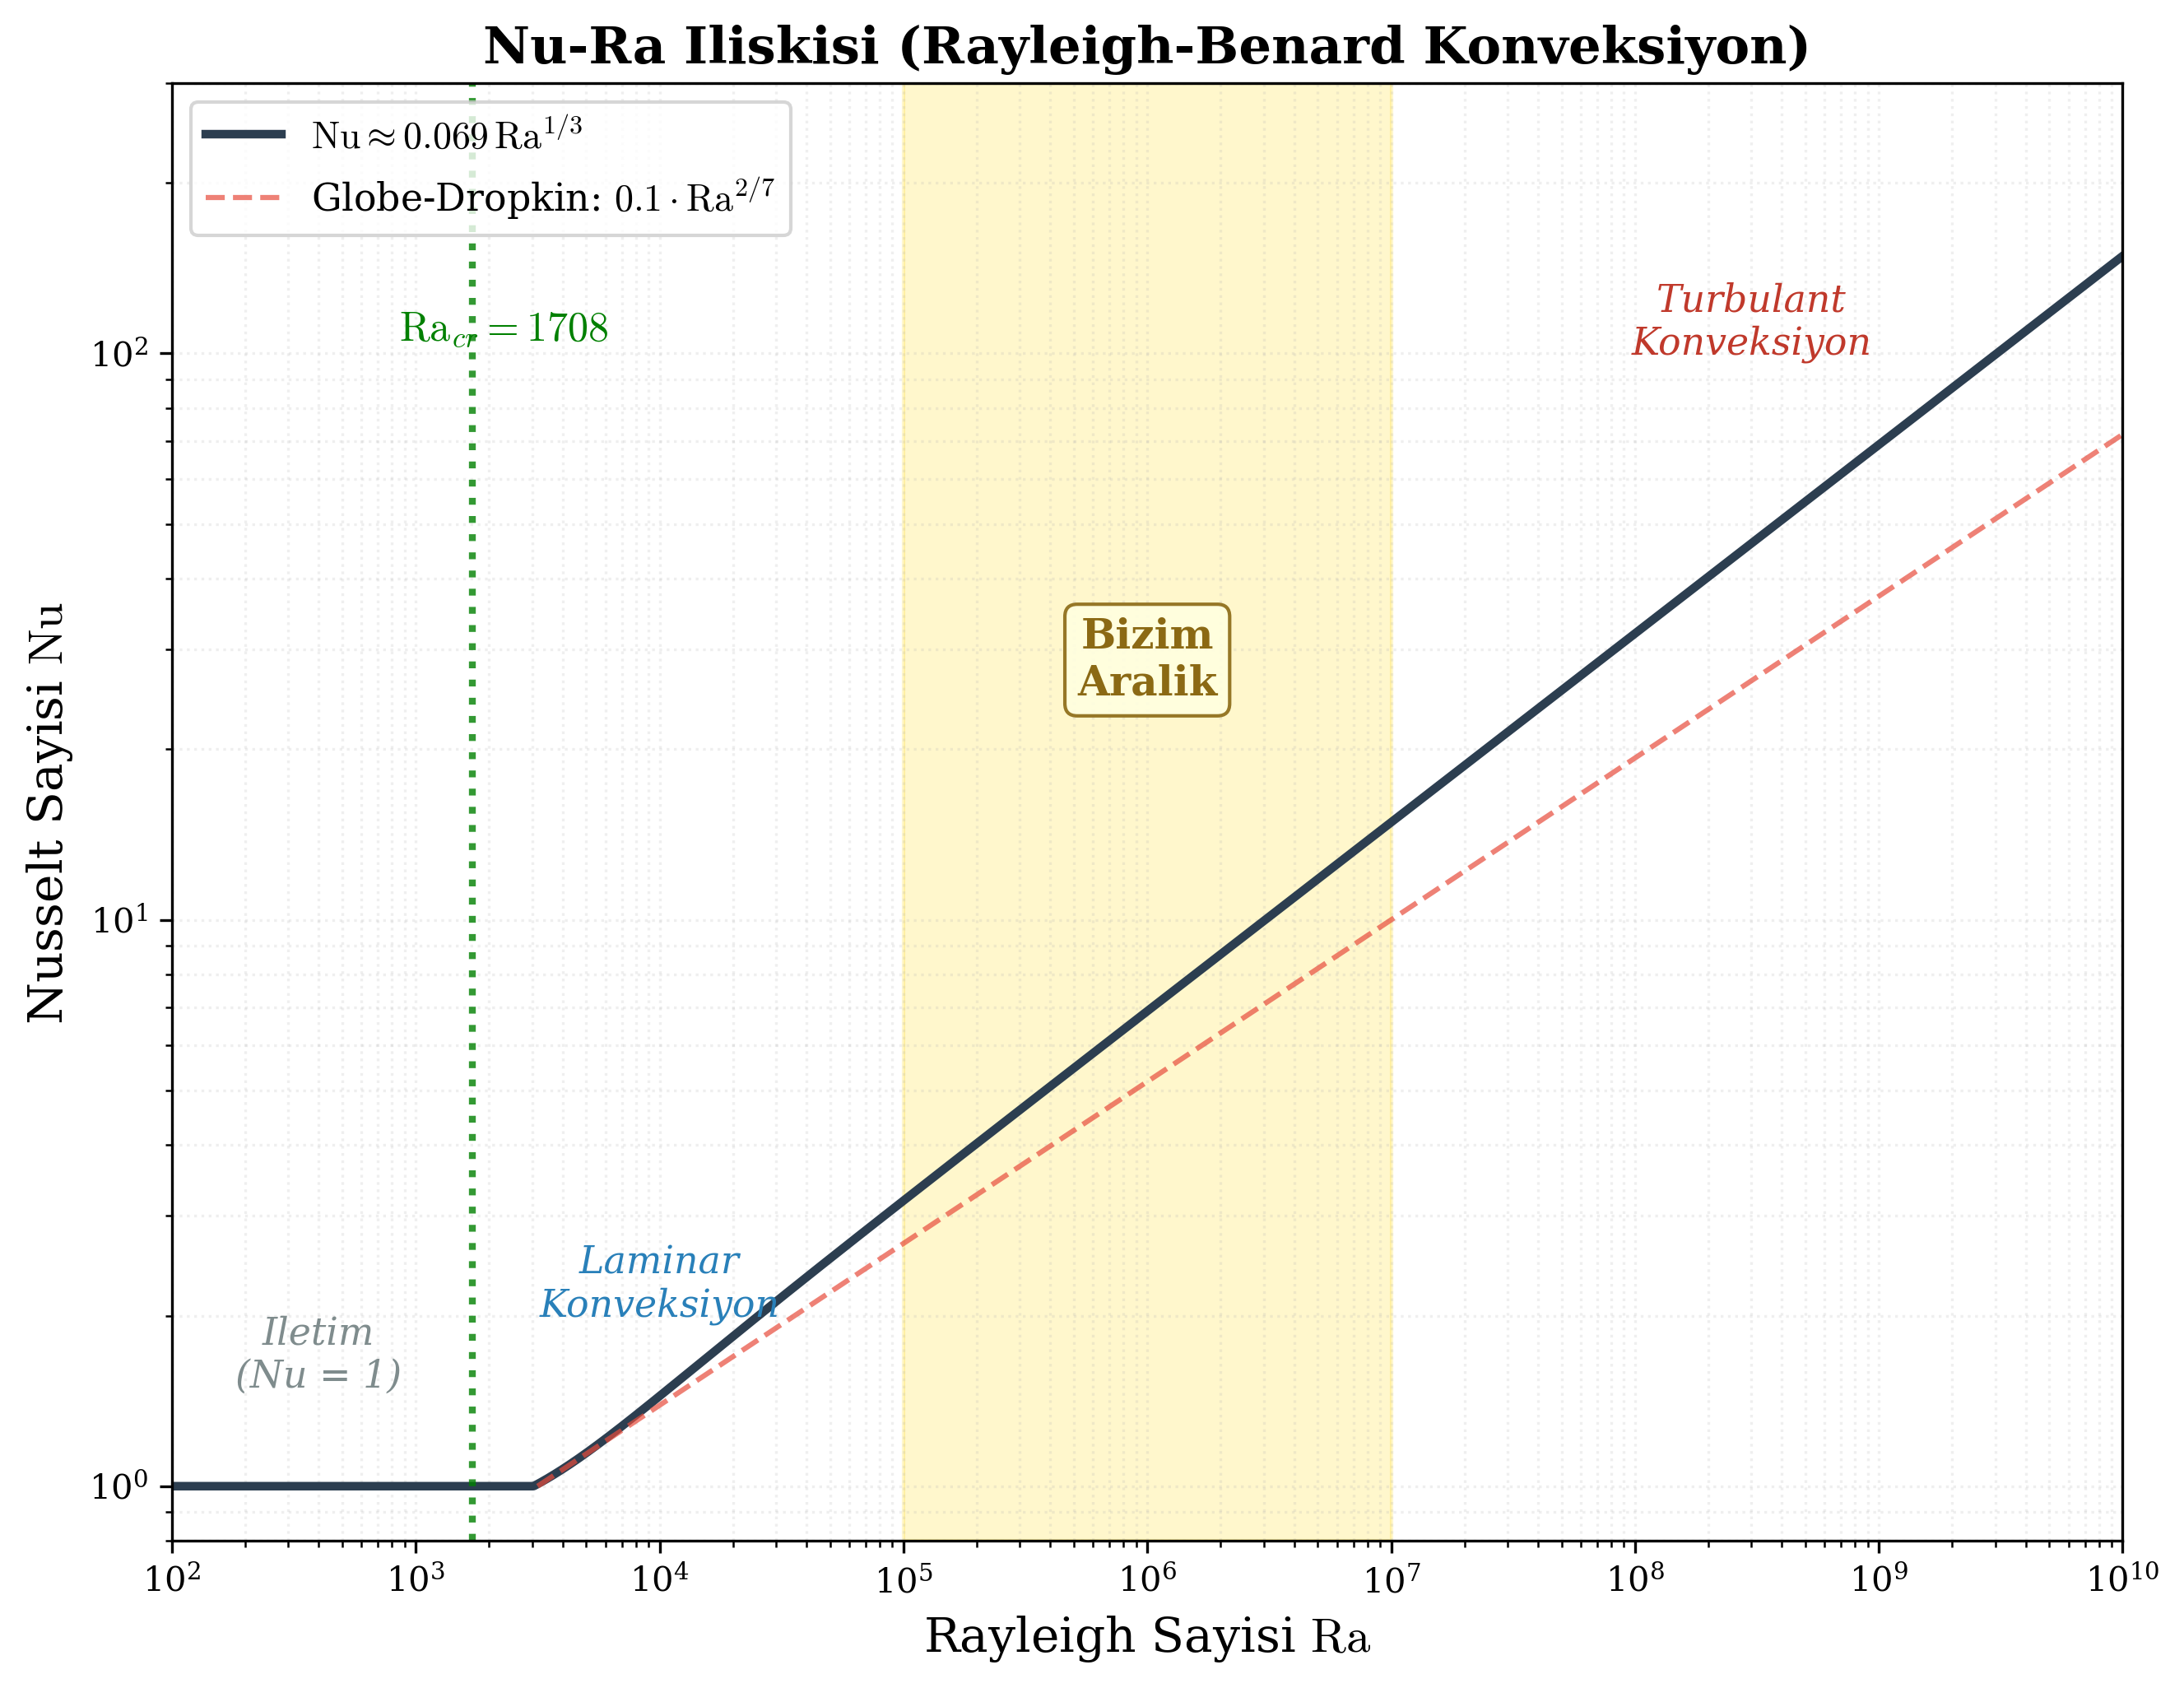
\includegraphics[width=0.8\textwidth]{nusselt_vs_ra.png}
\caption{Nusselt sayısının Rayleigh sayısına bağlılığı. $\Ray < 1708$'de saf iletim ($\Nus = 1$), üstünde konveksiyonla birlikte $\Nus \sim \Ray^{1/3}$. Bizim parametre aralığımız vurgulanmıştır.}
\label{fig:nusselt_vs_ra}
\end{figure}

% ============================================================
\section{Rejim Haritası}
\label{sec:rejim_haritasi}

Boyutsuz sayıların kombinasyonu, akış rejimini belirler. Aşağıdaki şema, $\Rey$--$\Ray$ düzleminde konveksiyon rejimlerini gösterir:

\begin{figure}[H]
    \centering
    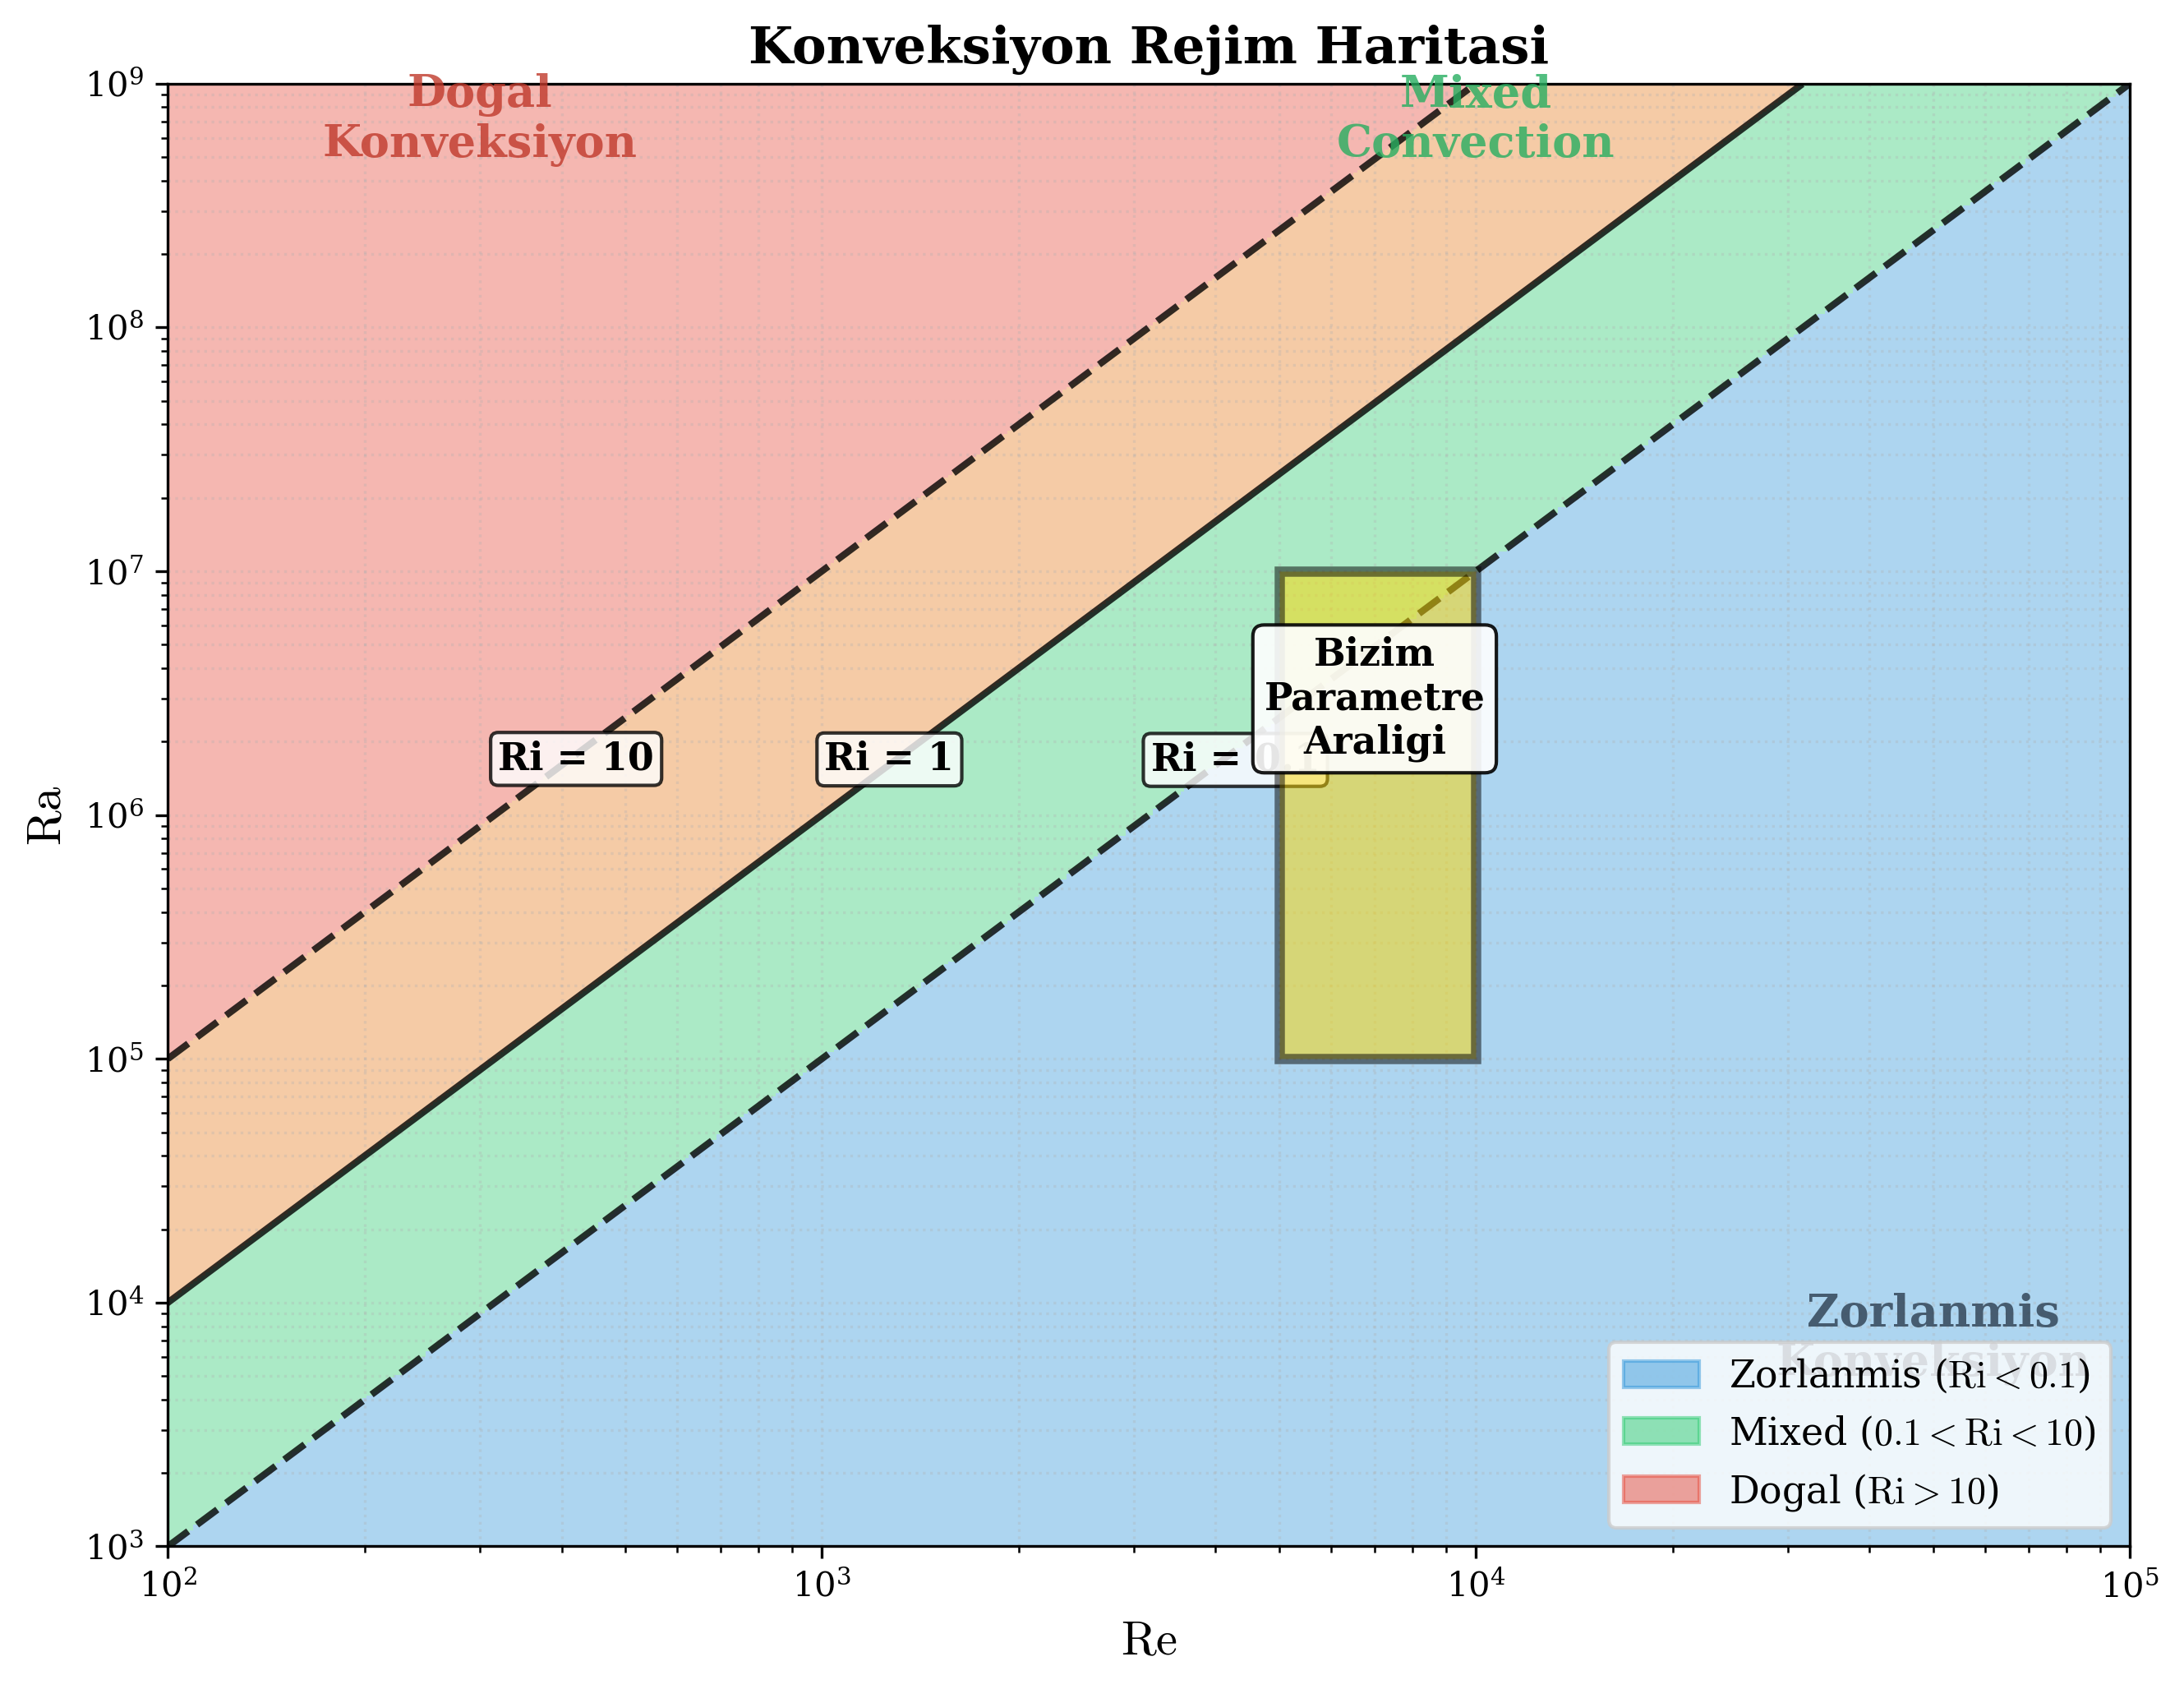
\includegraphics[width=0.8\textwidth]{regime_map.png}
    \caption{Konveksiyon rejim haritası. Eğri çizgi $\Rich = 1$ sınırını gösterir. Bu sınırın üstünde kaldırma kuvveti baskın (doğal konveksiyon), altında dış kuvvet baskın (zorlanmış konveksiyon). Aradaki bölge mixed convection'dır.}
    \label{fig:regime_map}
\end{figure}

$\Rich = 1$ eğrisini bulmak için $\Ray/(\Rey^2\Pran) = 1$ denkleminden:
\begin{equation}
    \Ray = \Pran\,\Rey^2
\end{equation}

Hava için ($\Pran = 0.71$): $\Ray_{\text{sınır}} = 0.71\,\Rey^2$. Örneğin $\Rey = 5000$ için $\Ray_{\text{sınır}} \approx 1.78 \times 10^7$.


% ============================================================
\section{Boyutsuz Denklem Sisteminin Özeti}
\label{sec:boyutsuz_ozet}

Yıldızları düşürelim (bundan sonra tüm değişkenler boyutsuz):

\begin{subequations}
\label{eq:nondim_system}
\begin{align}
    \pd{\vect{u}}{t} + (\vect{u}\cdot\gradient)\vect{u} &= -\gradient p + \frac{1}{\Rey}\laplacian\vect{u} + \Rich\,T\,\hat{\vect{e}}_y + \vect{F} \label{eq:nondim_mom_final} \\
    \pd{T}{t} + (\vect{u}\cdot\gradient)T &= \frac{1}{\Rey\,\Pran}\laplacian T \label{eq:nondim_ene_final} \\
    \divergence\vect{u} &= 0 \label{eq:nondim_cont_final}
\end{align}
\end{subequations}

Bu sistem 3 boyutsuz parametre ile tamamen tanımlanır: $\Rey$, $\Ray$ (veya $\Rich$), $\Pran$.

Bir sonraki bölümde, kaldırma teriminin ($\Rich\,T\,\hat{\vect{e}}_y$) nasıl Boussinesq yaklaşımından türediğini, bu yaklaşımın geçerlilik koşullarını ve konveksiyon türlerini detaylı inceleyeceğiz.

\chapter{Boussinesq Yaklaşımı ve Konveksiyon}
\label{ch:boussinesq}

% ============================================================
\section{Boussinesq Yaklaşımı Nedir?}
\label{sec:boussinesq_nedir}

Gerçek akışkanlarda sıcaklık değişimi yoğunluğu değiştirir. Sıcak hava hafifler, soğuk hava ağırlaşır. Tam sıkıştırılabilir denklemler bu etkiyi eksiksiz yakalar, ama çözümü çok pahalıdır (ses dalgalarını da çözmek gerekir).

Joseph Valentin Boussinesq (1903), basit ama güçlü bir yaklaşım önerdi:

\begin{definition}[Boussinesq Yaklaşımı]
Yoğunluk değişimi \textbf{yalnızca kaldırma (buoyancy) teriminde} hesaba katılır. Diğer tüm terimlerde yoğunluk sabit ($\rho_0$) alınır.
\end{definition}

Başka bir deyişle:
\begin{itemize}
    \item Süreklilik denkleminde: $\divergence\vect{u} = 0$ (sanki sıkıştırılamaz).
    \item Momentum denkleminde: Atalet terimi $\rho_0\,D\vect{u}/Dt$, viskoz terim $\mu\laplacian\vect{u}$ --- $\rho = \rho_0$ kullanılır.
    \item \textbf{Tek istisna:} Yerçekimi terimi $\rho\vect{g}$'de gerçek yoğunluk $\rho(T)$ kullanılır.
\end{itemize}

Bu ``tutarsız'' gibi görünebilir, ama fiziksel olarak gerekçelidir: yoğunluk değişimi küçüktür ($\Delta\rho/\rho_0 \ll 1$), atalet ve viskoz terimlerde ihmal edilebilir. Ama yerçekimi kuvveti $\rho g$ büyük bir sayıdır; küçük bir $\Delta\rho$ bile önemli bir kaldırma kuvveti yaratır.


% ============================================================
\section{Boussinesq Denklemlerinin Türetmesi}
\label{sec:boussinesq_turetme}

\textbf{Adım 1: Durum denklemi (lineer yaklaşım).}

Yoğunluğun sıcaklığa bağımlılığını birinci mertebe Taylor açılımıyla yazalım:
\begin{equation}
    \rho(T) = \rho_0 + \left.\pd{\rho}{T}\right|_{T_0} (T - T_0) + \mathcal{O}\bigl((T-T_0)^2\bigr)
    \label{eq:rho_taylor}
\end{equation}

Termal genleşme katsayısı tanımı:
\begin{equation}
    \beta \equiv -\frac{1}{\rho_0}\left.\pd{\rho}{T}\right|_{T_0}
    \label{eq:beta_def}
\end{equation}

Eksi işareti konvansiyondur: çoğu akışkanda sıcaklık arttıkça yoğunluk \textit{azalır}, yani $\partial\rho/\partial T < 0$; böylece $\beta > 0$ olur.

Denklem~\eqref{eq:rho_taylor}'ye yerleştirelim:
\begin{equation}
    \rho(T) = \rho_0\bigl[1 - \beta(T - T_0)\bigr]
    \label{eq:boussinesq_eos}
\end{equation}

\begin{example}
Hava için $\beta \approx 1/T_0$ (ideal gaz). $T_0 = 300$~K'de $\beta = 1/300 \approx 3.33 \times 10^{-3}$~K$^{-1}$.
\begin{itemize}
    \item $\Delta T = 20$~K: $\beta\Delta T = 0.067 \ll 1$ $\checkmark$ (Boussinesq geçerli)
    \item $\Delta T = 50$~K: $\beta\Delta T = 0.167$ (sınırda)
    \item $\Delta T = 200$~K: $\beta\Delta T = 0.667$ (Boussinesq geçersiz!)
\end{itemize}
\end{example}

\textbf{Adım 2: Momentum denklemine yerleştirme.}

Tam (sıkıştırılabilir) momentum denklemi:
\begin{equation}
    \rho\DDt{\vect{u}} = -\gradient p + \mu\laplacian\vect{u} + \rho\vect{g} + \vect{F}
\end{equation}

Sol taraftaki $\rho$'yu Boussinesq'e göre $\rho_0$ ile değiştirin (çünkü $\Delta\rho/\rho_0 \ll 1$):
\begin{equation}
    \rho_0\DDt{\vect{u}} = -\gradient p + \mu\laplacian\vect{u} + \rho(T)\,\vect{g} + \vect{F}
\end{equation}

\textbf{Adım 3: Yerçekimi teriminin işlenmesi.}

$\rho(T)\vect{g}$ terimini açalım. $\vect{g} = -g\,\hat{\vect{e}}_y$ (aşağı yönde):
\begin{equation}
    \rho(T)\,\vect{g} = \rho_0[1 - \beta(T-T_0)](-g\,\hat{\vect{e}}_y) = -\rho_0 g\,\hat{\vect{e}}_y + \rho_0 g\beta(T-T_0)\hat{\vect{e}}_y
\end{equation}

İlk terim ($-\rho_0 g\hat{\vect{e}}_y$) hidrostatik basınçla dengelenir. \textit{Değiştirilmiş basınç} tanımlayalım:
\begin{equation}
    p' = p + \rho_0 g\,y
    \label{eq:modified_pressure}
\end{equation}

O zaman $-\gradient p - \rho_0 g\,\hat{\vect{e}}_y = -\gradient p'$ olur.

\textbf{Adım 4: Boussinesq momentum denklemi.}

\begin{equation}
    \rho_0\DDt{\vect{u}} = -\gradient p' + \mu\laplacian\vect{u} + \rho_0 g\beta(T - T_{\text{ref}})\hat{\vect{e}}_y + \vect{F}
\end{equation}

$\rho_0$'a bölersek:
\begin{equation}
    \boxed{\pd{\vect{u}}{t} + (\vect{u}\cdot\gradient)\vect{u} = -\frac{1}{\rho_0}\gradient p' + \nu\laplacian\vect{u} + g\beta(T - T_{\text{ref}})\hat{\vect{e}}_y + \frac{\vect{F}}{\rho_0}}
    \label{eq:boussinesq_momentum}
\end{equation}

\textbf{Kaldırma terimi} $g\beta(T - T_{\text{ref}})\hat{\vect{e}}_y$'nin yapısına dikkat edin:
\begin{itemize}
    \item $T > T_{\text{ref}}$: Akışkan sıcak $\to$ kuvvet yukarı ($+y$) $\to$ yükselir.
    \item $T < T_{\text{ref}}$: Akışkan soğuk $\to$ kuvvet aşağı ($-y$) $\to$ alçalır.
    \item $T = T_{\text{ref}}$: Kaldırma yok.
\end{itemize}

\textbf{Adım 5: Tam Boussinesq sistemi.}

Enerji denklemi değişmez (zaten $\rho = \rho_0$ ile türetildi):
\begin{subequations}
\label{eq:boussinesq_system}
\begin{align}
    \pd{\vect{u}}{t} + (\vect{u}\cdot\gradient)\vect{u} &= -\frac{1}{\rho_0}\gradient p' + \nu\laplacian\vect{u} + g\beta(T - T_{\text{ref}})\hat{\vect{e}}_y + \frac{\vect{F}}{\rho_0} \label{eq:bouss_mom} \\
    \pd{T}{t} + (\vect{u}\cdot\gradient)T &= \kappa\laplacian T \label{eq:bouss_ene} \\
    \divergence\vect{u} &= 0 \label{eq:bouss_cont}
\end{align}
\end{subequations}

\begin{remark}
Boussinesq'te $\divergence\vect{u} = 0$ \textbf{kesindir}. Bu denklem bir ``yaklaşım'' değildir: yoğunluk etkisi \textbf{yalnızca} $g\beta(T-T_{\text{ref}})$ teriminde yer alır. Süreklilik denklemi ``sanki sıkıştırılamaz'' gibidir. Bu, sayısal çözüm için büyük kolaylıktır çünkü basınç Poisson denklemiyle hesaplanabilir.
\end{remark}


% ============================================================
\section{Rayleigh--B\'{e}nard Konveksiyonu}
\label{sec:rayleigh_benard}

\subsection{Problem Tanımı}

Rayleigh--Bénard (RB) konveksiyonu, doğal konveksiyonun en temel ve en çok çalışılan modelidir:

\begin{itemize}
    \item Yatay iki plaka arasında akışkan.
    \item Alt plaka sıcak ($T_h$), üst plaka soğuk ($T_c$).
    \item Yerçekimi aşağı yönde.
    \item Dış zorlama yok ($\vect{F} = 0$, $U = 0$).
\end{itemize}

Tek kontrol parametresi $\Ray$ (ve $\Pran$).

\subsection{Lineer Stabilite Analizi}

Hidrostatik denge (akışkan hareketsiz) çözümü:
\begin{equation}
    \vect{u}_0 = 0, \qquad T_0(y) = T_h - \frac{\Delta T}{H}\,y, \qquad p_0(y) = p_{\text{atm}} + \rho_0 g (H-y)
    \label{eq:hydrostatic}
\end{equation}

Bu çözüm her zaman vardır. Soru şu: bu denge \textit{kararlı} mı?

Küçük bir pertürbasyon ekleyelim:
\begin{equation}
    \vect{u} = \vect{u}_0 + \vect{u}' = \vect{u}', \qquad T = T_0 + T', \qquad p = p_0 + p'
\end{equation}

Boussinesq denklemlerine yerleştirip $\mathcal{O}({\vect{u}'}^2)$ terimlerini ihmal edelim (lineerizasyon):
\begin{subequations}
\begin{align}
    \pd{\vect{u}'}{t} &= -\frac{1}{\rho_0}\gradient p' + \nu\laplacian\vect{u}' + g\beta\,T'\hat{\vect{e}}_y \label{eq:perturb_mom} \\
    \pd{T'}{t} - \frac{\Delta T}{H}v' &= \kappa\laplacian T' \label{eq:perturb_ene} \\
    \divergence\vect{u}' &= 0 \label{eq:perturb_cont}
\end{align}
\end{subequations}

Denklem~\eqref{eq:perturb_ene}'deki $-(\Delta T/H)v'$ terimi kilit terimdir: dikey hız pertürbasyonu $v'$ temel sıcaklık gradyanıyla etkileşerek sıcaklık pertürbasyonu üretir.

Normal mod analizi ($\vect{u}', T', p' \propto e^{\sigma t + i(k_x x + k_z z)}$) uygulanır ve $y$ yönünde uygun sınır koşulları ile bir \textbf{özdeğer problemi} elde edilir.

\subsection{Kritik Rayleigh Sayısı}

Lineer stabilite analizi sonucu:
\begin{equation}
    \boxed{\Ray_{\text{cr}} = \frac{27}{4}\pi^4 \approx 657.5 \quad \text{(free-slip)}}
    \label{eq:ra_cr_freeslip}
\end{equation}
\begin{equation}
    \boxed{\Ray_{\text{cr}} = 1707.76 \approx 1708 \quad \text{(no-slip)}}
    \label{eq:ra_cr_noslip}
\end{equation}

\begin{itemize}
    \item $\Ray < \Ray_{\text{cr}}$: Tüm pertürbasyonlar söner ($\sigma < 0$). Akışkan hareketsiz, $T$ doğrusal profilde kalır. Isı yalnızca iletimle taşınır: $\Nus = 1$.
    \item $\Ray = \Ray_{\text{cr}}$: Nötr kararlılık ($\sigma = 0$). Sonlu genlikli konveksiyon hücreleri oluşmaya başlar.
    \item $\Ray > \Ray_{\text{cr}}$: Pertürbasyonlar büyür ($\sigma > 0$). Konveksiyon başlar.
\end{itemize}

\subsection{Konveksiyon Yapıları}

$\Ray$ arttıkça akış yapıları zenginleşir:

\begin{enumerate}
    \item $\Ray \gtrsim \Ray_{\text{cr}}$: \textbf{Düzenli konveksiyon hücreleri.} 2B'de ``rolls'' (silindirler), 3B'de altıgen Bénard hücreleri. Sıcak akışkan yükselir, soğuyan akışkan alçalır.

    \item $\Ray \sim 10^4$--$10^5$: Hücreler kararsızlaşır. Zaman bağımlı davranış. Osilatörler, periyot-ikilemeleri.

    \item $\Ray \gtrsim 10^6$: \textbf{Türbülant konveksiyon.} Büyük ölçekli sirkulasyon (LSC) + türbülant plume'lar. Alt sınır tabakasından sıcak plume'lar kopup yükselir; üst sınır tabakasından soğuk plume'lar düşer.

    \item $\Ray \gtrsim 10^{10}$--$10^{14}$: ``Ultimate'' rejim tartışması. Sınır tabakaları kendileri türbülant mı oluyor? Açık araştırma sorusu.
\end{enumerate}


% ============================================================
\section{Zorlanmış Konveksiyon}
\label{sec:forced_convection}

Zorlanmış konveksiyonda akışkan hareketi dış kuvvetle sağlanır ve kaldırma kuvveti ihmal edilebilir ($\Rich \ll 1$).

Bu durumda sıcaklık denklemi \textbf{pasif skaler} gibi davranır:
\begin{subequations}
\begin{align}
    \pd{\vect{u}}{t} + (\vect{u}\cdot\gradient)\vect{u} &= -\frac{1}{\rho_0}\gradient p + \nu\laplacian\vect{u} + \frac{\vect{F}}{\rho_0} \\
    \pd{T}{t} + (\vect{u}\cdot\gradient)T &= \kappa\laplacian T \\
    \divergence\vect{u} &= 0
\end{align}
\end{subequations}

Dikkat: Momentum denkleminde $T$ yok. Hız alanı sıcaklıktan bağımsız çözülür; sonra sıcaklık dağılımı bilinen $\vect{u}$ ile bulunur. Bu tek yönlü bağlantıdır ve çözümü kolaylaştırır.

\subsection{Kolmogorov Forcing}

Bu projede kullanılan rüzgâr etkisi, \textbf{Kolmogorov forcing} ile modellenmiştir:
\begin{equation}
    \vect{F} = A\,\sin\!\left(k_f\,\frac{2\pi y}{L_y}\right)\hat{\vect{e}}_x
    \label{eq:kolmogorov_forcing}
\end{equation}

Burada:
\begin{itemize}
    \item $A$: Forcing genliği [m/s$^2$]
    \item $k_f$: Forcing dalga sayısı (genellikle $k_f = 1$)
    \item Kuvvet yalnızca $x$ yönünde ve $y$'ye sinüzoidal bağımlı
\end{itemize}

Neden bu forcing?
\begin{enumerate}
    \item \textbf{Analitik laminar çözüm vardır:} $u_{\text{lam}}(y) \propto \sin(k_f y)$. Bu, validasyon için kullanılabilir.
    \item \textbf{Enerji enjeksiyonu kontrollüdür:} Tek bir dalga sayısında enerji pompalanır, enerji kaskadı temiz çalışır.
    \item \textbf{Periyodik sınır koşullarıyla uyumludur:} $\sin$ fonksiyonu doğal olarak periyodiktir.
\end{enumerate}


% ============================================================
\section{Mixed Convection}
\label{sec:mixed_convection}

Mixed convection, zorlanmış ve doğal konveksiyonun \textit{birlikte} etkili olduğu rejimdir. $\Rich \sim \mathcal{O}(1)$ olduğunda ne kaldırma kuvveti ne de dış zorlama ihmal edilebilir.

\subsection{Fiziksel Yapılar}

\begin{figure}[H]
\centering
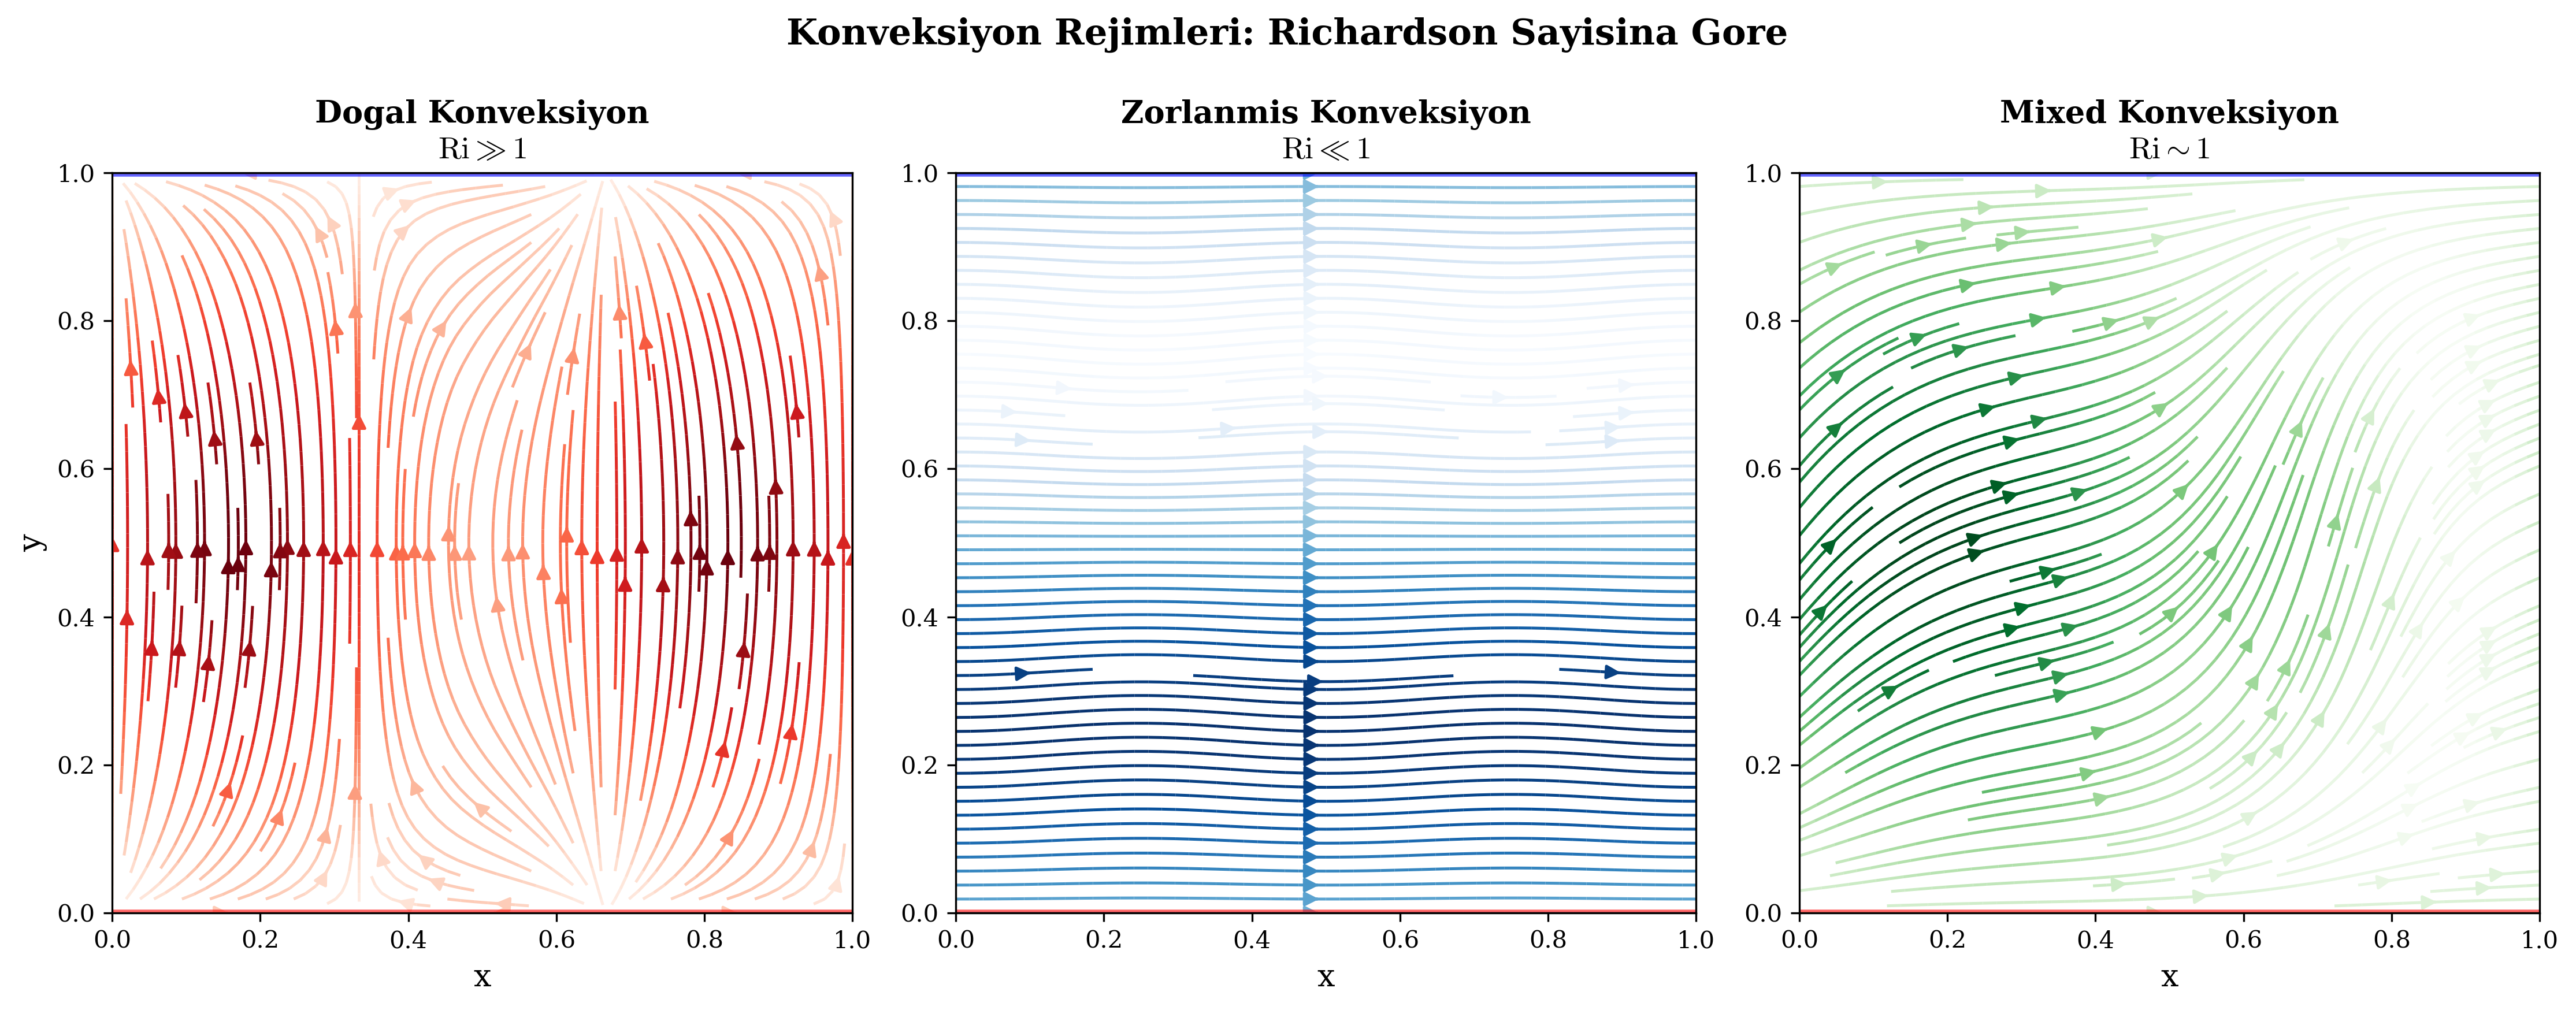
\includegraphics[width=\textwidth]{convection_types.png}
\caption{Üç konveksiyon rejimi: (sol) doğal konveksiyon ($\Rich \gg 1$, dikey plume'lar), (orta) zorlanmış konveksiyon ($\Rich \ll 1$, yatay akış), (sağ) mixed convection ($\Rich \sim 1$, eğik plume'lar ve karmaşık yapılar).}
\label{fig:convection_types}
\end{figure}

Mixed convection'da karmaşık akış yapıları ortaya çıkar:

\begin{enumerate}
    \item \textbf{Eğik plume'lar (tilted plumes):} Doğal konveksiyonda plume'lar dikey yükselir. Yatay rüzgâr onları yatırır. Plume açısı $\sim \arctan(\Rich^{1/2})$ ile ölçeklenir.

    \item \textbf{Kesilmiş konveksiyon hücreleri (sheared cells):} Bénard hücreleri rüzgâr tarafından deforme edilir. Rüzgâr yönünde uzar, dikey yönde sıkışır.

    \item \textbf{Büyük ölçekli sirkulasyon (LSC) + rüzgâr etkileşimi:} Doğal konveksiyonun yarattığı LSC ile dış akış etkileşir. Aynı yönde iseler güçlenir, ters yönde iseler zayıflar veya salınır.

    \item \textbf{Rejim geçişleri:} Parametre uzayında keskin olmayan geçişler. Küçük $\Delta\Ray$ değişimi akış yapısını tamamen değiştirebilir (histerezis mümkün).
\end{enumerate}

\subsection{Neden Zor?}

Mixed convection modellemesi zordur çünkü:
\begin{enumerate}
    \item \textbf{İki yönlü bağlantı:} Hız $\leftrightarrow$ sıcaklık. Bağımsız çözülemez.
    \item \textbf{Çoklu zaman ölçekleri:} Advektif zaman ölçeği $H/U$ ve kaldırma zaman ölçeği $H/\sqrt{g\beta\Delta T H}$ farklı olabilir.
    \item \textbf{Çoklu uzunluk ölçekleri:} Hız sınır tabakası, sıcaklık sınır tabakası, plume kalınlığı, forcing dalga boyu\ldots
    \item \textbf{3B etkileri güçlü:} 2B modeller yanıltıcı olabilir (spanwise instability, 3B plume etkileşimleri).
\end{enumerate}

\subsection{Literatürdeki Durum}

\begin{itemize}
    \item 2B RB konveksiyonu DNS ile kapsamlı çalışılmıştır ($\Ray$ = $10^6$--$10^{15}$).
    \item 3B RB konveksiyonu DNS ile $\Ray \lesssim 10^{10}$ kadar çalışılmıştır.
    \item Mixed convection (RB + forced) 2B'de sınırlı çalışma var.
    \item \textbf{3B mixed convection + neural operator: neredeyse çalışılmamış.} Bu, projemizin orijinal katkısıdır.
\end{itemize}


% ============================================================
\section{Non-Boussinesq Etkileri}
\label{sec:non_boussinesq}

\subsection{Boussinesq'in Sınırları}

Boussinesq yaklaşımı $\beta\Delta T \ll 1$ koşulunda geçerlidir. Bu koşul bozulduğunda:

\begin{enumerate}
    \item \textbf{Yoğunluk asimetrisi:} Sıcak ve soğuk plume'lar farklı davranır. Soğuk akışkan daha ağırdır, daha hızlı düşer. Sıcak akışkan daha hafiftir, daha yavaş yükselir. Bu asimetri Boussinesq'te yoktur.

    \item \textbf{Viskozite değişimi:} Gerçek akışkanlarda viskozite sıcaklıkla değişir. Hava için $\mu \propto T^{0.7}$. Bu da asimetriye katkıda bulunur.

    \item \textbf{Sıkıştırılamazlık bozulması:} $\divergence\vect{u} \neq 0$ olur. Stratifiye akışlarda bu önemli olabilir.
\end{enumerate}

\subsection{Ne Zaman Gerekir?}

\begin{center}
\begin{tabular}{rcl}
\toprule
$\beta\Delta T$ & \textbf{Durum} & \textbf{Yaklaşım} \\
\midrule
$< 0.1$ & Güvenli & Boussinesq yeterli \\
$0.1$--$0.2$ & Sınırda & Dikkatli değerlendirme gerekli \\
$> 0.2$ & Tehlikeli & Non-Boussinesq veya sıkıştırılabilir \\
\bottomrule
\end{tabular}
\end{center}

\begin{example}
Hava ($\beta = 1/T_0 = 1/300$~K$^{-1}$) için:
\begin{itemize}
    \item $\Delta T = 20$~K: $\beta\Delta T = 0.067$ $\to$ Boussinesq güvenle geçerli.
    \item $\Delta T = 50$~K: $\beta\Delta T = 0.167$ $\to$ Sınırda. Non-Boussinesq etkileri görülebilir.
    \item $\Delta T = 100$~K: $\beta\Delta T = 0.333$ $\to$ Boussinesq yetersiz.
\end{itemize}
Bu projede $\Delta T = 20$~K civarında çalışıyoruz, dolayısıyla Boussinesq geçerlidir.
\end{example}

\subsection{Non-Boussinesq Denklemler}

Tam non-Boussinesq formülasyon, yoğunluğu sıcaklığın fonksiyonu olarak tutar:
\begin{equation}
    \rho = \frac{\rho_0 T_0}{T} \quad \text{(ideal gaz)}
    \label{eq:non_bouss_eos}
\end{equation}

Bu durumda süreklilik denklemi:
\begin{equation}
    \pd{\rho}{t} + \divergence(\rho\vect{u}) = 0 \quad \text{ve genel olarak} \quad \divergence\vect{u} \neq 0
\end{equation}

Ancak düşük Mach sayısı ($\mathrm{Ma} \ll 1$) koşulunda ``low-Mach yaklaşımı'' kullanılabilir:
\begin{itemize}
    \item Akustik dalgalar filtrelenir (ses hızı $\to \infty$).
    \item Basınç, termodinamik ($p_0$) ve dinamik ($p'$) kısımlara ayrılır.
    \item $p_0$ uzayda sabit (kapalı kap) veya zamanda sabit (açık akış).
    \item Süreklilik denklemi: $\divergence\vect{u} = -(1/T)\,DT/Dt$ (sıfır değil!).
\end{itemize}

Non-Boussinesq modelleme, bu projenin ileri aşamasında (Boussinesq çalıştıktan sonra) bir genişletme hedefi olarak düşünülmektedir. INNATE mimarisine non-Boussinesq nöronları eklemek prensipte mümkündür.


% ============================================================
\section{Bölüm Özeti}
\label{sec:boussinesq_ozet}

\begin{enumerate}
    \item \textbf{Boussinesq yaklaşımı:} Yoğunluk değişimi yalnızca kaldırma teriminde. Geçerlilik: $\beta\Delta T \ll 1$.

    \item \textbf{Boussinesq denklemleri:}
    \begin{align*}
        \pd{\vect{u}}{t} + (\vect{u}\cdot\gradient)\vect{u} &= -\frac{1}{\rho_0}\gradient p + \nu\laplacian\vect{u} + g\beta(T-T_{\text{ref}})\hat{\vect{e}}_y + \frac{\vect{F}}{\rho_0} \\
        \pd{T}{t} + (\vect{u}\cdot\gradient)T &= \kappa\laplacian T \\
        \divergence\vect{u} &= 0
    \end{align*}

    \item \textbf{Rayleigh--Bénard:} Alttan ısıtma, üstten soğutma. $\Ray_{\text{cr}} \approx 1708$ (no-slip). $\Ray > \Ray_{\text{cr}}$ $\to$ konveksiyon.

    \item \textbf{Mixed convection:} Zorlanmış + doğal birlikte. $\Rich \sim \mathcal{O}(1)$. En karmaşık rejim.

    \item \textbf{Bu projede:} Boussinesq + Kolmogorov forcing + RB ısıtma $\to$ 3B mixed convection. $\Rey = 1000$--$10{,}000$, $\Ray = 10^5$--$10^7$, $\Pran = 0.71$.
\end{enumerate}

\chapter{Spectral Yöntemler}
\label{ch:spectral}

Bu bölümde, periyodik sınır koşullarında PDE çözümünün en güçlü yöntemlerinden biri olan \textbf{spectral yöntemler}i inceliyoruz.
Temel fikir basit: fonksiyonu Fourier uzayina taşi, türev almak yerine çarpım yap, sonra geri dön.
Bu yaklaşim, sonlu fark (finite difference) yöntemlerine kiyasla \emph{üstel yakinsama} (exponential convergence) sağlar.


% ============================================================
\section{Fourier Serileri}
\label{sec:fourier_serileri}

\subsection{Gerçel Form}

Periyodik bir $f(x)$ fonksiyonunu ($f(x+L) = f(x)$) trigonometrik fonksiyonlarin toplami olarak yazabiliriz:

\begin{equation}
\label{eq:fourier_reel}
f(x) = \frac{a_0}{2} + \sum_{n=1}^{\infty} \left[ a_n \cos\!\left(\frac{2\pi n x}{L}\right) + b_n \sin\!\left(\frac{2\pi n x}{L}\right) \right]
\end{equation}

Burada $L$ periyot, $a_n$ ve $b_n$ Fourier katsayilari:
\begin{align}
a_n &= \frac{2}{L} \int_0^L f(x)\cos\!\left(\frac{2\pi n x}{L}\right) dx, \label{eq:an} \\
b_n &= \frac{2}{L} \int_0^L f(x)\sin\!\left(\frac{2\pi n x}{L}\right) dx. \label{eq:bn}
\end{align}

\begin{remark}
$a_0/2$ terimi fonksiyonun \textbf{ortalama değeri}dir: $a_0/2 = \frac{1}{L}\int_0^L f(x)\,dx$.
\end{remark}

\subsection{Kompleks (Exponential) Form}

Euler bağintisi $e^{i\theta} = \cos\theta + i\sin\theta$ kullanilarak, gerçel form çok daha zarif bir biçimde yazilabilir. $\cos$ ve $\sin$ terimlerini birleştirelim:
\begin{align}
a_n\cos(k_n x) + b_n\sin(k_n x) &= \frac{a_n - ib_n}{2}\,e^{ik_n x} + \frac{a_n + ib_n}{2}\,e^{-ik_n x}
\end{align}
Burada $k_n = 2\pi n / L$ dalga sayisidir. $\hat{c}_n \equiv (a_n - ib_n)/2$ tanimlanirsa:

\begin{equation}
\boxed{f(x) = \sum_{n=-\infty}^{\infty} \hat{c}_n \, e^{i k_n x}, \qquad k_n = \frac{2\pi n}{L}}
\label{eq:fourier_complex}
\end{equation}

\textbf{Fourier katsayilari} ortogonallik bağintisi $\frac{1}{L}\int_0^L e^{ik_n x}e^{-ik_m x}dx = \delta_{nm}$ kullanilarak:
\begin{equation}
\boxed{\hat{c}_n = \frac{1}{L}\int_0^{L} f(x)\,e^{-ik_n x}\,dx}
\label{eq:fourier_coeff}
\end{equation}

Bu kompleks form, türev alma işlemini dramatik biçimde basitleştirecek.


% ============================================================
\section{Ayrik Fourier Dönüşümü (DFT)}
\label{sec:dft}

Bilgisayarda sürekli Fourier integralini hesaplayamayız. Onun yerine fonksiyonu $N$ ayrik noktada örnekleriz.

\subsection{Grid Tanimlamasi}

$[0, L)$ araligini eşit araliklara bölelim:
\begin{equation}
x_j = j\,\Delta x, \qquad j = 0, 1, \ldots, N-1, \qquad \Delta x = \frac{L}{N}
\label{eq:grid}
\end{equation}

\begin{remark}
$N$ nokta ile $x_0 = 0$ ve $x_{N-1} = L - \Delta x$ olur. $x_N = L$ noktasi dahil \emph{edilmez} çünkü periyodik siniir koşulunda $f(0) = f(L)$ olduğundan bu nokta $x_0$ ile aynidir.
\end{remark}

\subsection{DFT Tanimi}

Sürekli Fourier integralinin ayrik karşiliği:

\begin{equation}
\boxed{\hat{f}_k = \sum_{j=0}^{N-1} f_j \, e^{-2\pi i j k / N}, \qquad k = 0, 1, \ldots, N-1}
\label{eq:dft}
\end{equation}

Ters dönüşüm (IDFT):
\begin{equation}
\boxed{f_j = \frac{1}{N}\sum_{k=0}^{N-1} \hat{f}_k \, e^{2\pi i j k / N}, \qquad j = 0, 1, \ldots, N-1}
\label{eq:idft}
\end{equation}

\begin{remark}
$1/N$ normalizasyonu IDFT'de. Bazi kaynaklarda (ve NumPy/PyTorch'ta) DFT'de $1/\sqrt{N}$ kullanilir. \textbf{Tutarlilik önemli}: DFT$\cdot$IDFT $= $ identity olmalı.
\end{remark}

\subsection{Dalga Sayilari ve Nyquist Frekansi}

$N$ noktayla temsil edilebilecek dalga sayilari sinirlidir:
\begin{equation}
k_n = \frac{2\pi n}{L}, \qquad n = -\frac{N}{2}, \ldots, -1, 0, 1, \ldots, \frac{N}{2} - 1
\label{eq:wavenumbers}
\end{equation}

\textbf{Nyquist frekansi}: temsil edilebilecek en yüksek frekans
\begin{equation}
k_{\max} = \frac{2\pi}{L}\cdot\frac{N}{2} = \frac{\pi}{\Delta x}
\label{eq:nyquist}
\end{equation}

Fiziksel yorum: en az 2 grid noktasi ile temsil edilebilecek en kisa dalga boyu $\lambda_{\min} = 2\Delta x$'tir.
Bu, \textbf{Shannon-Nyquist örnekleme teoremi}nin doğrudan sonuçudur.


% ============================================================
\section{FFT Algoritmasi}
\label{sec:fft}

\subsection{Hesaplama Karmaşıklığı}

DFT'yi (\ref{eq:dft}) doğrudan hesaplamak:
\begin{itemize}
\item Her $\hat{f}_k$ için $N$ çarpma + $N$ toplama $\Rightarrow$ toplam $O(N^2)$ işlem.
\item $N = 10^6$ için $10^{12}$ işlem --- pratik değil.
\end{itemize}

\subsection{Cooley-Tukey (1965): Böl ve Yönet}

FFT (Fast Fourier Transform), DFT'yi $O(N \log N)$'e düşüren algoritmadir.
Temel fikir: $N$-nokta DFT'yi iki $N/2$-nokta DFT'ye böl:

\begin{align}
\hat{f}_k &= \sum_{j=0}^{N-1} f_j\, e^{-2\pi i jk/N} \notag \\
&= \underbrace{\sum_{m=0}^{N/2-1} f_{2m}\, e^{-2\pi i mk/(N/2)}}_{\text{{çift indeksler}}: \; E_k}
\;+\;
e^{-2\pi ik/N}\;\underbrace{\sum_{m=0}^{N/2-1} f_{2m+1}\, e^{-2\pi i mk/(N/2)}}_{\text{tek indeksler}: \; O_k}
\label{eq:fft_decomp}
\end{align}

Yani:
\begin{equation}
\hat{f}_k = E_k + W^k \cdot O_k, \qquad W = e^{-2\pi i / N}\;\text{(twiddle factor)}
\label{eq:butterfly}
\end{equation}

Bu bölüme rekürsif olarak uygulanir:
\begin{equation}
\underbrace{N}_{\text{DFT}} \to 2\times\frac{N}{2} \to 4\times\frac{N}{4} \to \cdots \to N\times 1
\qquad \Rightarrow \quad \log_2 N \;\text{seviye} \times N \;\text{işlem/seviye} = O(N\log N)
\end{equation}

\begin{example}
Hiz karşilastirmasi ($N = 96 \times 160 \times 64 = 983{,}040$ --- bizim grid):
\begin{itemize}
\item Dogrudan DFT: $N^2 \approx 10^{12}$ işlem
\item FFT: $N\log_2 N \approx 2\times10^7$ işlem
\item \textbf{Hizlanma}: $\sim 50{,}000\times$
\end{itemize}
\end{example}

\subsection{3D FFT}

Üç boyutlu DFT, her boyutta ardisik 1D FFT'ler olarak hesaplanir (tensor çarpimi yapisi):
\begin{equation}
\hat{f}(k_x, k_y, k_z) = \text{FFT}_z\!\Big(\text{FFT}_y\!\big(\text{FFT}_x\!\big(f(x,y,z)\big)\big)\Big)
\end{equation}

PyTorch'ta tek satirla:
\begin{lstlisting}[caption={3D FFT PyTorch'ta},label={lst:fft3d}]
import torch.fft as fft
f_hat = fft.fftn(f, dim=(-3, -2, -1))  # 3 boyutta FFT
\end{lstlisting}


% ============================================================
\section{Spectral Türev Hesaplama}
\label{sec:spectral_deriv}

Spectral yöntemlerin as gizli silahi: \textbf{türev almak, Fourier uzayinda çarpmaya dönüşür}.

\begin{figure}[H]
\centering
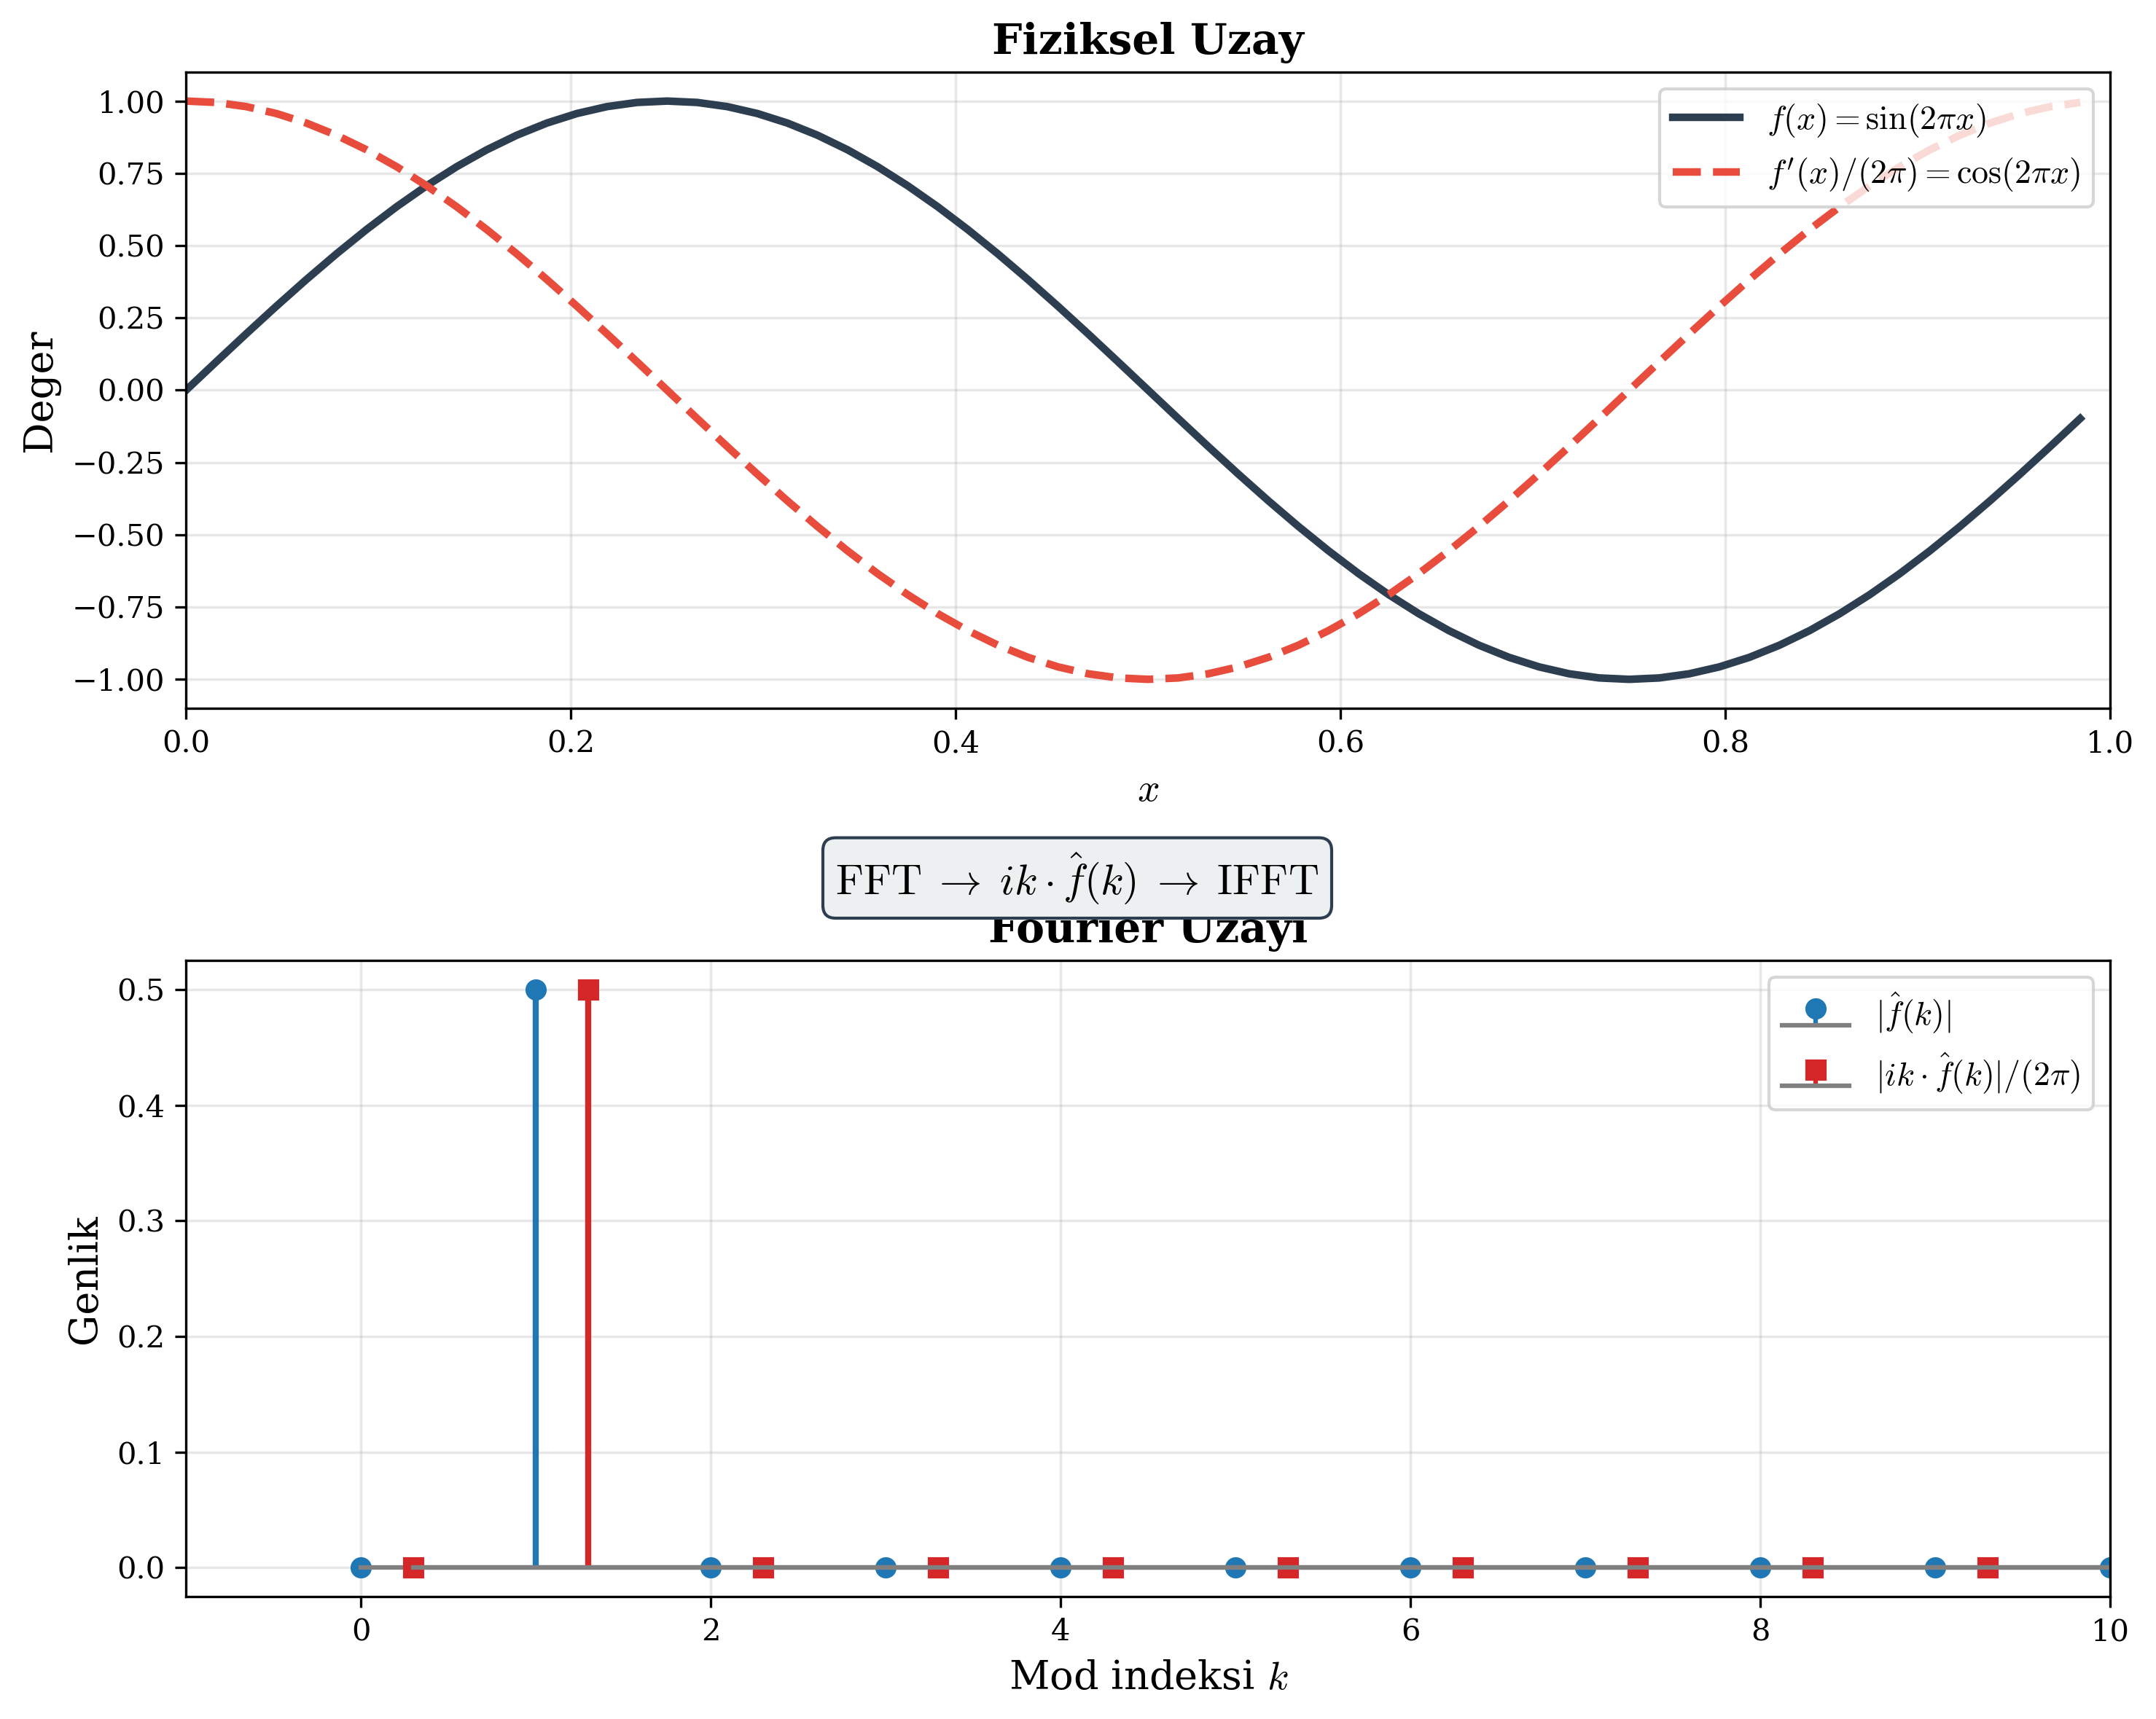
\includegraphics[width=0.85\textwidth]{spectral_derivative.png}
\caption{Spectral türev hesaplama: fiziksel uzayda $f(x)$ ve $f'(x)$ (üst), Fourier uzayinda $|\hat{f}(k)|$ ve $|ik\hat{f}(k)|$ (alt). FFT $\to$ $ik$ ile çarpma $\to$ IFFT.}
\label{fig:spectral_derivative}
\end{figure}

\subsection{Temel Teorem: Birinci Türev}

\begin{theorem}[Spectral Türev]
\label{thm:spectral_deriv}
$f(x)$ periyodik ve pürüzsüz bir fonksiyon olsun. O zaman:
\begin{equation}
\boxed{f'(x) = \mathcal{F}^{-1}\!\big[\,ik\cdot\hat{f}(k)\,\big]}
\label{eq:spectral_deriv}
\end{equation}
Yani: $f'(x) = \text{IFFT}\big(ik \cdot \text{FFT}(f)\big)$
\end{theorem}

\begin{proof}[Türetme]
Fourier serisi temsili ile baslayalim:
\begin{equation}
f(x) = \sum_{n=-\infty}^{\infty} \hat{c}_n\, e^{ik_n x}
\end{equation}

Her iki tarafi $x$'e gore türetelim. Toplam ve türev yer değiştirebilir (üniform yakinsama):
\begin{align}
f'(x) &= \frac{d}{dx}\sum_{n=-\infty}^{\infty}\hat{c}_n\,e^{ik_n x} \notag \\
&= \sum_{n=-\infty}^{\infty}\hat{c}_n\cdot\frac{d}{dx}e^{ik_n x} \notag \\
&= \sum_{n=-\infty}^{\infty}\hat{c}_n\cdot (ik_n)\,e^{ik_n x} \notag \\
&= \sum_{n=-\infty}^{\infty}\underbrace{(ik_n\,\hat{c}_n)}_{\widehat{f'}(k_n)}\,e^{ik_n x}
\label{eq:spectral_deriv_proof}
\end{align}

Sonuçu okuyalim: $f'(x)$'in Fourier katsayilari $ik_n\,\hat{c}_n$'dir. Yani \textbf{türev almak} = \textbf{Fourier katsayisini $ik$ ile çarpmak}.
\end{proof}

\subsection{İkinci Türev}

Ayni mantigi iki kez uygulayelim:
\begin{align}
f''(x) &= \frac{d}{dx}f'(x) = \frac{d}{dx}\sum_n (ik_n)\hat{c}_n\,e^{ik_n x} \notag \\
&= \sum_n (ik_n)^2\,\hat{c}_n\,e^{ik_n x} = \sum_n (-k_n^2)\,\hat{c}_n\,e^{ik_n x}
\end{align}

\begin{equation}
\boxed{f''(x) = \mathcal{F}^{-1}\!\big[-k^2 \cdot \hat{f}(k)\big]}
\label{eq:spectral_2nd_deriv}
\end{equation}

Genel olarak $m$-inci türev:
\begin{equation}
\frac{d^m f}{dx^m} = \mathcal{F}^{-1}\!\big[(ik)^m \cdot \hat{f}(k)\big]
\label{eq:spectral_mth_deriv}
\end{equation}

\subsection{3D'de Gradient ve Laplacian}

Üç boyutlu $f(x,y,z)$ fonksiyonu için her yöndeki türev bağimsiz olarak hesaplanir. $\hat{f}(k_x,k_y,k_z)$ 3D Fourier dönüşümünü göstersin:

\textbf{Gradient:}
\begin{equation}
\pd{f}{x} = \mathcal{F}^{-1}\!\big[ik_x\cdot\hat{f}(k_x,k_y,k_z)\big], \qquad
\pd{f}{y} = \mathcal{F}^{-1}\!\big[ik_y\cdot\hat{f}\big], \qquad
\pd{f}{z} = \mathcal{F}^{-1}\!\big[ik_z\cdot\hat{f}\big]
\label{eq:3d_gradient}
\end{equation}

\textbf{Laplacian:}
\begin{align}
\laplacian f &= \pdd{f}{x} + \pdd{f}{y} + \pdd{f}{z} \notag \\
&= \mathcal{F}^{-1}\!\big[(-k_x^2)\hat{f}\big] + \mathcal{F}^{-1}\!\big[(-k_y^2)\hat{f}\big] + \mathcal{F}^{-1}\!\big[(-k_z^2)\hat{f}\big] \notag \\
&= \mathcal{F}^{-1}\!\big[-(k_x^2 + k_y^2 + k_z^2)\cdot\hat{f}\big]
\end{align}

\begin{equation}
\boxed{\laplacian f = \mathcal{F}^{-1}\!\Big[-|\vect{k}|^2 \cdot \hat{f}(\vect{k})\Big], \qquad |\vect{k}|^2 = k_x^2 + k_y^2 + k_z^2}
\label{eq:spectral_laplacian_3d}
\end{equation}

\subsection{Sayisal Örnek}

$L = 2\pi$ periyotlu $f(x) = \sin(2\pi x / L) = \sin(x)$ fonksiyonunun türevi $f'(x) = \cos(x)$ olduğunu biliyoruz. Spectral yöntemle doğrulayalım:

\begin{enumerate}
\item $f(x) = \sin(x)$ fonksiyonunun Fourier dönüşümü:
\begin{equation}
\sin(x) = \frac{e^{ix} - e^{-ix}}{2i} \qquad\Rightarrow\qquad \hat{c}_1 = \frac{1}{2i} = -\frac{i}{2},\quad \hat{c}_{-1} = \frac{i}{2}
\end{equation}
\item $ik$ ile çarpalim ($k_1 = 1$, $k_{-1} = -1$):
\begin{align}
ik_1 \cdot \hat{c}_1 &= i\cdot 1 \cdot\left(-\frac{i}{2}\right) = -\frac{i^2}{2} = \frac{1}{2} \\
ik_{-1}\cdot\hat{c}_{-1} &= i\cdot(-1)\cdot\frac{i}{2} = -\frac{i^2}{2} = \frac{1}{2}
\end{align}
\item Ters dönüşüm:
\begin{equation}
f'(x) = \frac{1}{2}\,e^{ix} + \frac{1}{2}\,e^{-ix} = \cos(x) \quad\checkmark
\end{equation}
\end{enumerate}


% ============================================================
\section{Anizotropik Domain}
\label{sec:anisotropic}

\subsection{Bizim Problem Geometrisi}

Projemizdeki periyodik kutu eşit kenarli değil:
\begin{equation}
\text{Domain:}\quad L_x = 6, \quad L_y = 10, \quad L_z = 4
\end{equation}
\begin{equation}
\text{Grid:}\quad N_x = 96, \quad N_y = 160, \quad N_z = 64
\end{equation}

\subsection{Yöne Bagli Dalga Sayilari}

Her yönün kendi periyodu ve grid çözünürlüğü oldugundan, dalga sayilari yönden yöne değişir:
\begin{equation}
k_x^{(n)} = \frac{2\pi n}{L_x}, \qquad
k_y^{(m)} = \frac{2\pi m}{L_y}, \qquad
k_z^{(l)} = \frac{2\pi l}{L_z}
\label{eq:aniso_wavenumbers}
\end{equation}

\begin{example}
Sayisal degerler:
\begin{itemize}
\item $x$ yonunde: $\Delta k_x = 2\pi/6 \approx 1.047$, \quad $k_{x,\max} = \pi N_x/L_x = \pi\cdot96/6 \approx 50.3$
\item $y$ yonunde: $\Delta k_y = 2\pi/10 \approx 0.628$, \quad $k_{y,\max} = \pi\cdot160/10 \approx 50.3$
\item $z$ yonunde: $\Delta k_z = 2\pi/4 \approx 1.571$, \quad $k_{z,\max} = \pi\cdot64/4 \approx 50.3$
\end{itemize}

Grid orani $N/L$ her yonde esit tutulmustur ($96/6 = 160/10 = 64/4 = 16$), bu da fiziksel cozunurlugu her yonde esitler.
\end{example}

\subsection{PyTorch Implementasyonu}

\texttt{innate.py} icerisindeki \texttt{SpectralOps3DAniso} sinifi tam olarak bu anizotropik yapıyı uygular:

\begin{lstlisting}[caption={SpectralOps3DAniso dalga sayisi hesabi},label={lst:aniso_wavenumbers}]
# Her yon icin ayri dalga sayisi dizisi
kx_1d = torch.fft.fftfreq(Nx, d=Lx/Nx) * 2*pi  # d = dx = Lx/Nx
ky_1d = torch.fft.fftfreq(Ny, d=Ly/Ny) * 2*pi
kz_1d = torch.fft.fftfreq(Nz, d=Lz/Nz) * 2*pi

# 3D meshgrid
kx, ky, kz = torch.meshgrid(kx_1d, ky_1d, kz_1d, indexing='ij')
\end{lstlisting}

\begin{remark}
PyTorch'un \texttt{fftfreq(N, d=dx)} fonksiyonu $[0, 1, 2, \ldots, N/2-1, -N/2, \ldots, -1] / (N \cdot dx)$ dondurur. $2\pi$ ile carpmak, fiziksel dalga sayisi $k_n = 2\pi n/L$'yi verir.
\end{remark}

\subsubsection{Nyquist Modu Sifirlama}

\texttt{SpectralOps3DAniso}'da ek bir incelik vardir: \textbf{Nyquist modunun sifirlanmasi}.
\begin{lstlisting}[caption={Nyquist modu sifirlama}]
if Nx % 2 == 0:
    kx_1d[Nx // 2] = 0.0  # Nyquist modu sifirla
\end{lstlisting}

$N$ cift iken $k_{N/2}$ modu belirsizdir: $e^{i\pi j}$ hem $\cos(\pi j)$ hem $-\cos(\pi j)$ olarak yorumlanabilir. Türev hesabinda $ik_{N/2}\hat{f}_{N/2}$ terimi yalancı (spurious) bir salınım yaratır. Sifirlamak bu ambiguity'yi yok eder ve türevin gerçel kalmasini garantiler.


% ============================================================
\section{De-aliasing}
\label{sec:dealiasing}

\subsection{Problem: Nonlineer Terimlerde Aliasing}

\begin{figure}[H]
\centering
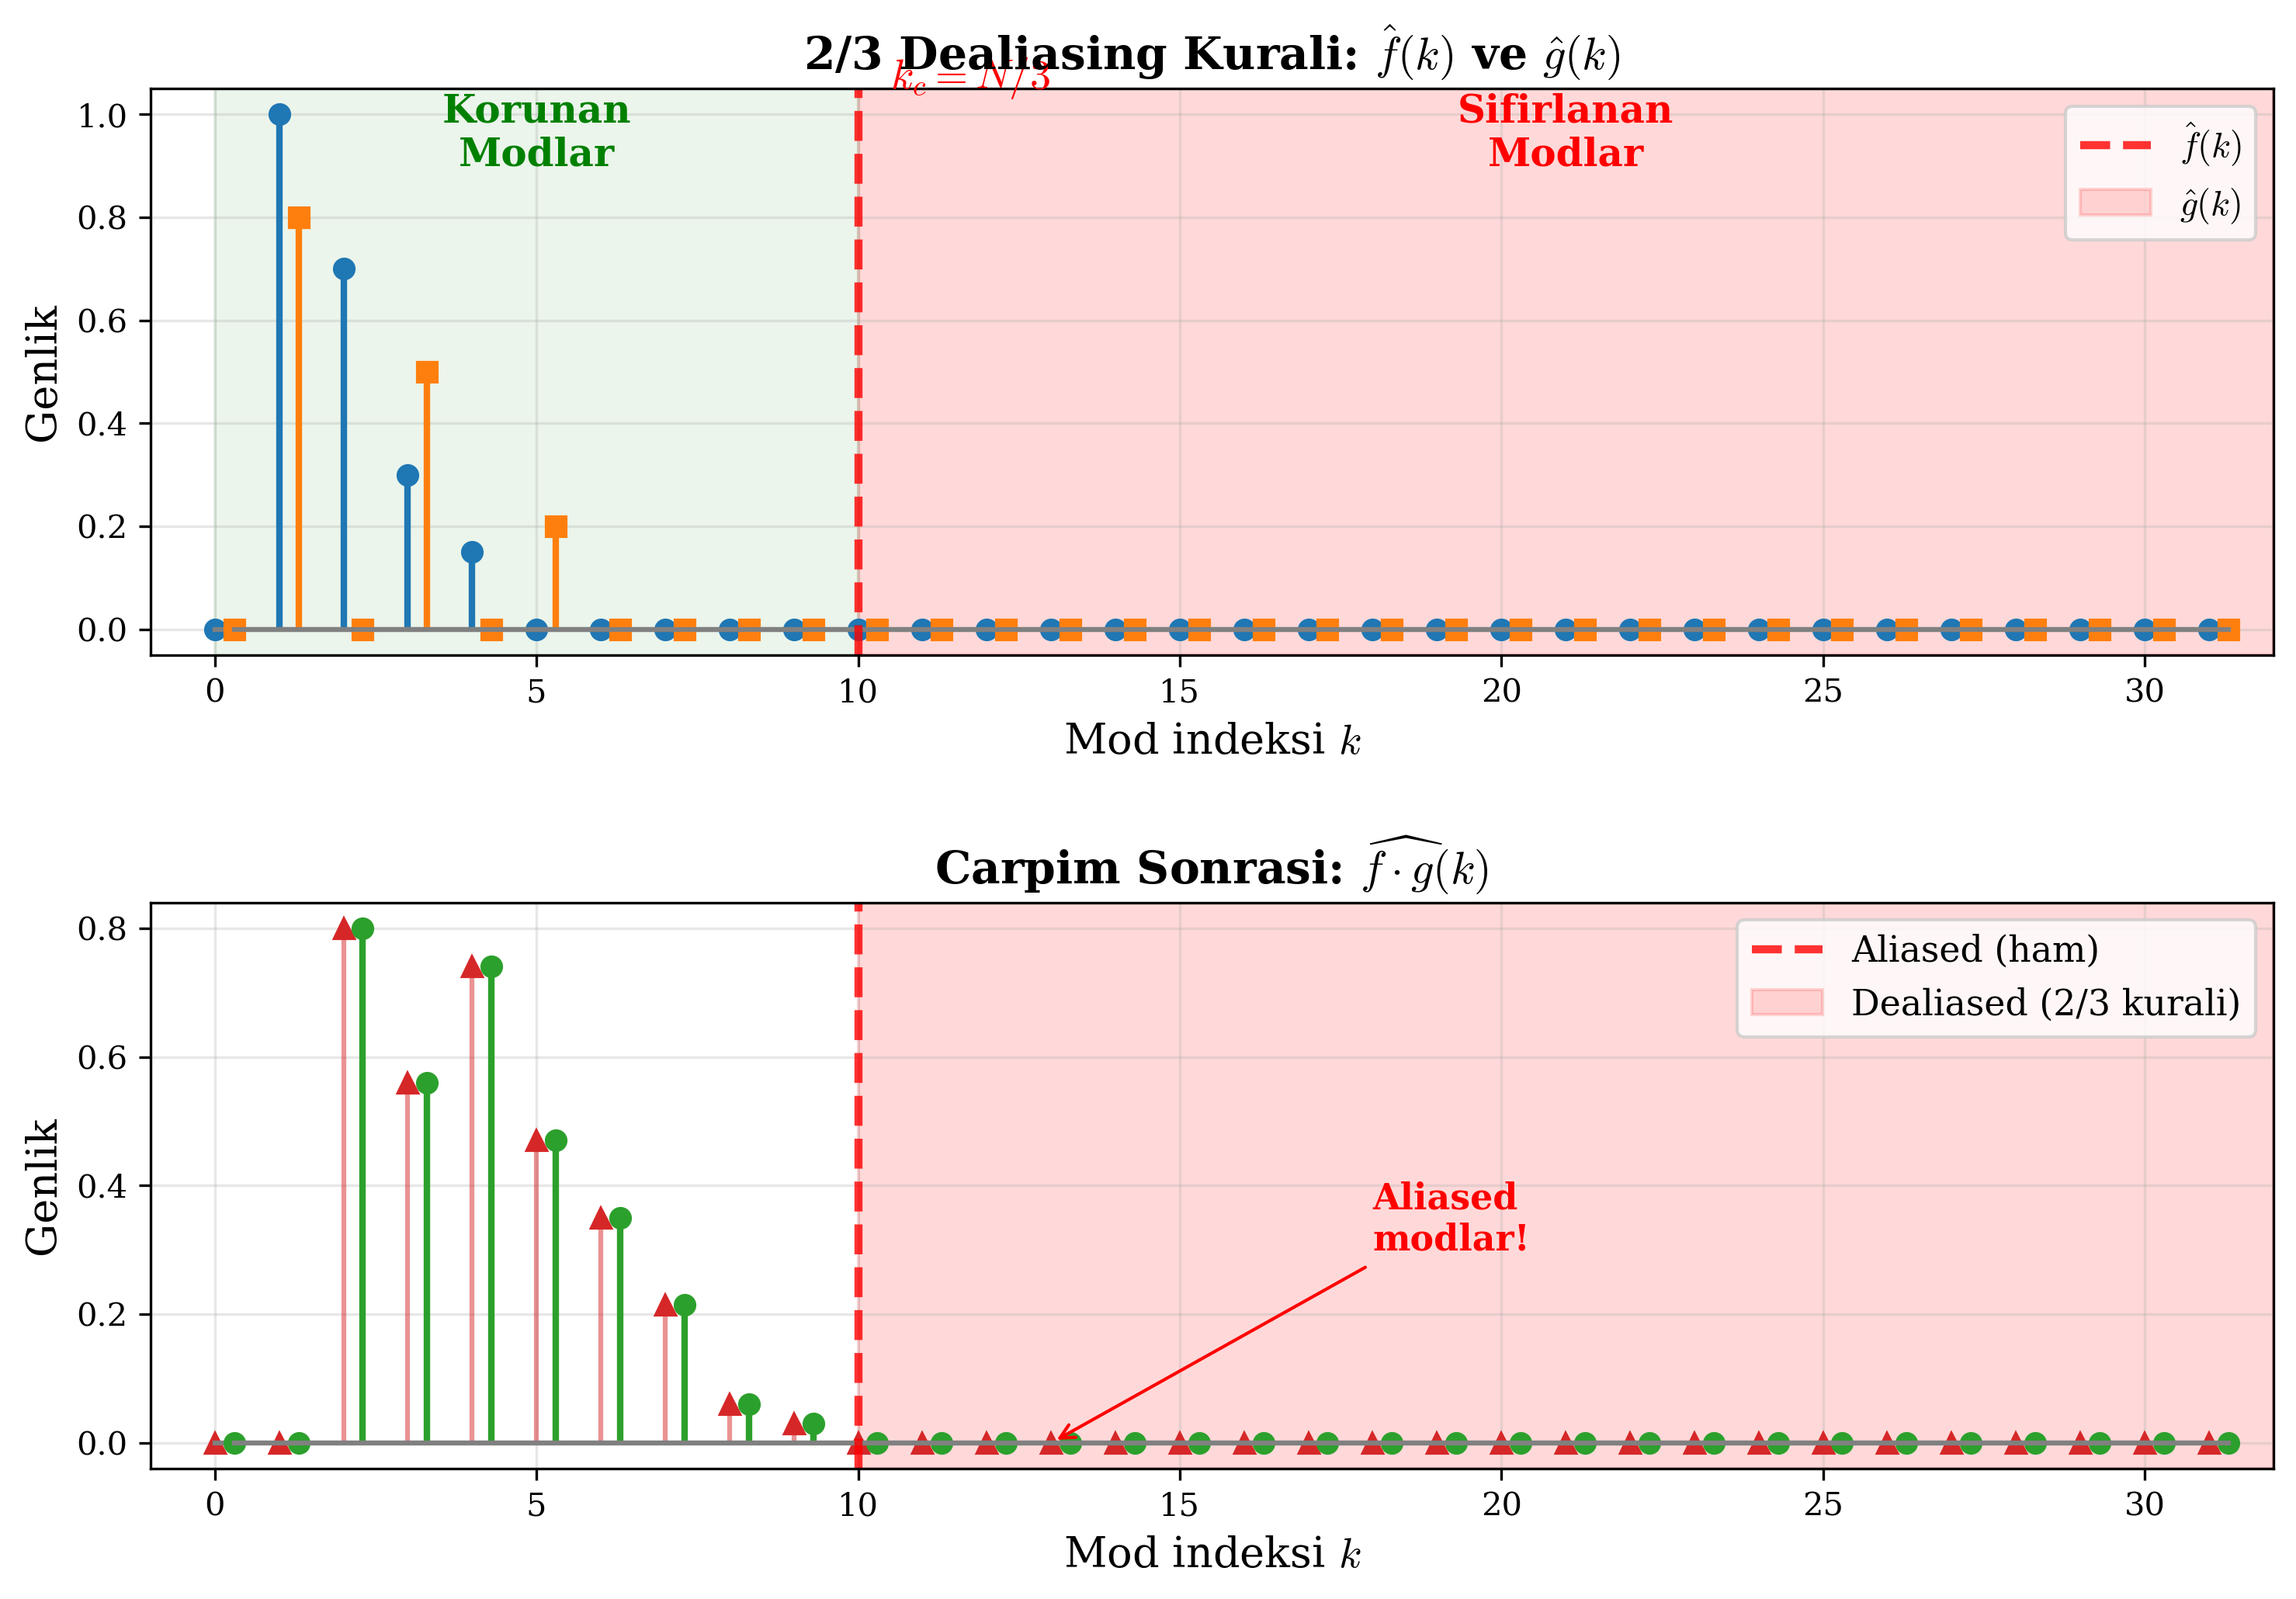
\includegraphics[width=0.85\textwidth]{dealiasing.png}
\caption{De-aliasing: 2/3 kuralı. $|k| > N/3$ olan modlar sıfırlanır (kırmızı bölge). Bu, nonlineer çarpım sonrası aliasing hatasını önler.}
\label{fig:dealiasing}
\end{figure}

Navier-Stokes denklemindeki adveksiyon terimi $(\vect{u}\cdot\gradient)\vect{u}$ \textbf{nonlineerdir}: hız alanının kendisiyle çarpımı. Bu çarpım, Fourier uzayında \textbf{konvolüsyon}a karşılık gelir.

İki Fourier modunun carpimini düşünelim:
\begin{equation}
e^{ik_m x}\cdot e^{ik_n x} = e^{i(k_m + k_n)x}
\end{equation}

Eğer $|k_m| \leq k_{\max}$ ve $|k_n| \leq k_{\max}$ ise, çarpim $|k_m + k_n| \leq 2k_{\max}$ dalga sayisina sahip olabilir. Ama bizim gridimiz sadece $|k| \leq k_{\max} = N/2$'ye kadar temsil edebilir. $N/2 < |k_m + k_n| \leq N$ arasindaki modlar ne olur?

\textbf{Aliasing}: Temsil edilemeyen yüksek frekansli mod, düşük frekansli bir moda ``katlanir'':
\begin{equation}
e^{i(k_m + k_n)x_j} = e^{i(k_m + k_n - 2\pi N/L)x_j} \qquad\text{(grid üzerinde ayirt edilemez)}
\end{equation}

Bu, \textbf{sahte enerji} yaratir ve say\i{}sal çözümü bozar.

\subsection{2/3 Kurali --- Türetme}
\label{subsec:twothirds}

Aliasing'i önlemenin en yaygin yöntemi \textbf{2/3 kurali} (Orszag, 1971): hesaplamadan önce $|k| > N/3$ olan modlari sifirla.

\textbf{Neden tam olarak $N/3$?} Adim adim:

\begin{enumerate}
\item Carpimdan önce her iki çarpanin da $|k| \leq K$ modlari olsun.
\item Carpim sonucu $|k| \leq 2K$ modlari içerecektir.
\item Aliasing olmasin diye carpim sonucu gridin temsil sinirinda kalmali: $2K \leq k_{\max} = N/2$.
\item Dolayisyla $K \leq N/4$.
\end{enumerate}

Bir dakika --- bu $N/4$ verir, ama pratikte $N/3$ kullaniliyor. Fark şuradan gelir: padded convolution ile degil, \emph{truncated} Fourier uzayinda çalisiyoruz. Daha dikkatli analiz:

\begin{enumerate}
\item Fonksiyonlarimiz $[-N/2, N/2)$ arasinda modlara sahip.
\item $|k| > N/3$ modlarini sifirliyoruz, yani aktif modlar $|k| \leq N/3$.
\item İki aktif mod çarpimi: $|k_m + k_n| \leq 2N/3$.
\item $2N/3 < N/2$ olmadigi için aliasing olabilir, \emph{ama} $2N/3 < N$ oldugundan katlanma $N - 2N/3 = N/3$'ten büyük modlara gider --- bunlar zaten sifir!
\item Yani aliased enerji zaten sifirlanmis modlara duuser ve gerçek modlari \emph{kirletmez}.
\end{enumerate}

\begin{equation}
\boxed{\text{De-aliasing:}\quad \hat{f}_k = 0 \;\;\text{for}\;\; |k| > \frac{N}{3}}
\label{eq:dealias_rule}
\end{equation}

\begin{remark}
Etkin çözünürlük: $N = 96$ noktamiz varsa, sadece $N/3 = 32$ mod kullaniriz. Bu da cozunurlugun \%67'sini \emph{kullanmak}, \%33'ünü \emph{feda etmek} demektir. Pahali ama zorunlu.
\end{remark}

\subsection{3/2 Kurali (Padding Yöntemi)}

Alternatif yaklasim: çözünürlük kaybetmek yerine, çarpimi daha büyük bir gridde yap:

\begin{enumerate}
\item Fourier katsayilarini $3N/2$ boyutlu bir diziye zero-pad et.
\item $3N/2$ boyutlu IFFT ile fiziksel uzaya dön.
\item Fiziksel uzayda çarpımı yap ($f\cdot g$ noktasal).
\item $3N/2$ boyutlu FFT ile geri dön.
\item $|k| > N/2$ modlarini at, $N$ boyutuna geri dön.
\end{enumerate}

Bu yöntem hiç mod kaybettirmez ama \%50 daha fazla bellek ve hesaplama gerektirir. Pratikte iki yöntem birbirine denk sonuçlar verir.

\subsection{Kodda De-aliasing}

\texttt{SpectralOps3DAniso} icerisinde 2/3 kurali uygulamasi:
\begin{lstlisting}[caption={De-aliasing mask olusturma},label={lst:dealias}]
# Mod indeksleri uzerinden 2/3 kurali
mx = torch.fft.fftfreq(Nx, d=1.0) * Nx  # [-N/2, ..., N/2-1]
my = torch.fft.fftfreq(Ny, d=1.0) * Ny
mz = torch.fft.fftfreq(Nz, d=1.0) * Nz
Mx, My, Mz = torch.meshgrid(mx, my, mz, indexing='ij')

dealias_mask = (
    (torch.abs(Mx) < Nx // 3) &
    (torch.abs(My) < Ny // 3) &
    (torch.abs(Mz) < Nz // 3)
)
\end{lstlisting}


% ============================================================
\section{Poisson Denklemi Spectral Çözümü}
\label{sec:poisson}

\subsection{Problem}

Navier-Stokes çözümünde her zaman adiminda Poisson denklemi çözülmelidir:
\begin{equation}
\laplacian p = f \qquad\text{(verilen kaynak terimi $f$)}
\label{eq:poisson}
\end{equation}

Sonlu fark yöntemlerinde bu, büyük bir lineer sistem ($Ap = f$) demektir --- iteratif çözücü (CG, GMRES, multigrid) gerektirir. Spectral yöntemde ise \textbf{dogrudan çözüm} mümkündür.

\subsection{Türetme}

Her iki tarafa 3D FFT uygulayalim:
\begin{align}
\laplacian p = f \qquad &\xrightarrow{\text{FFT}} \qquad -(k_x^2 + k_y^2 + k_z^2)\,\hat{p} = \hat{f} \notag \\
&\xrightarrow{\text{çöz}} \qquad \hat{p}(\vect{k}) = \frac{-\hat{f}(\vect{k})}{|\vect{k}|^2}
\label{eq:poisson_spectral}
\end{align}

\begin{equation}
\boxed{p = \mathcal{F}^{-1}\!\left[\frac{-\hat{f}(\vect{k})}{k_x^2 + k_y^2 + k_z^2}\right]}
\label{eq:poisson_solution}
\end{equation}

\subsection{$k = 0$ Modu}

$\vect{k} = (0,0,0)$ için payda sifir olur. Bu mod fonksiyonun \textbf{uzaysal ortalamasi}dir:
\begin{equation}
\hat{p}(0,0,0) = \frac{1}{\text{Vol}}\int_\Omega p\,dV \equiv \langle p \rangle
\end{equation}

Periyodik siniir kosullarinda basinc $p$'ye bir sabit eklemek fizigi değiştirmez (çünkü sadece $\gradient p$ görülür). Bu yüzden:
\begin{equation}
\hat{p}(0,0,0) = 0 \qquad\text{(ortalama basinc sifir)}
\label{eq:mean_pressure}
\end{equation}

\subsection{Pressure Projection (Helmholtz Ayrismasi)}
\label{subsec:projection}

Navier-Stokes çözümünde kritik bir adim: hız alanını \textbf{divergence-free} (sıkıştırılamaz) yapmak.

\textbf{Helmholtz Ayrismasi Teoremi}: Her (pürüzsüz) vektör alan $\vect{v}$ iki bilesene ayrilabilir:
\begin{equation}
\vect{v} = \underbrace{\vect{u}}_{\text{solenoidal}\;(\divergence\vect{u}=0)} + \underbrace{\gradient\phi}_{\text{irrotasyonel}\;(\curl\gradient\phi=0)}
\label{eq:helmholtz}
\end{equation}

Projection (Chorin, 1968): divergence-free olmayan $\vect{v}$'den solenoidal $\vect{u}$'yu cikarma:
\begin{enumerate}
\item Divergence hesapla: $d = \divergence\vect{v}$
\item Poisson çöz: $\laplacian\phi = d$
\item Gradient çikar: $\vect{u} = \vect{v} - \gradient\phi$
\end{enumerate}

Spectral uzayda tamami tek satirda:
\begin{equation}
\hat{\vect{u}} = \hat{\vect{v}} - \frac{\vect{k}(\vect{k}\cdot\hat{\vect{v}})}{|\vect{k}|^2}
\label{eq:leray_projection}
\end{equation}

Bu \textbf{Leray projeksiyon operatörüdür}: $\mathbb{P} = \mathbb{I} - \vect{k}\vect{k}^T / |\vect{k}|^2$.

\begin{lstlisting}[caption={Spectral Poisson çözümü ve projection},label={lst:poisson}]
import torch.fft as fft

# Poisson cozumu: nabla^2 p = rhs
rhs_hat = fft.fftn(rhs)
k_sq = kx**2 + ky**2 + kz**2
k_sq_safe = k_sq.clone()
k_sq_safe[k_sq_safe == 0] = 1.0    # Divide-by-zero onle

p_hat = rhs_hat / (-k_sq_safe)
p_hat[..., 0, 0, 0] = 0.0          # Ortalama basinc = 0
p = fft.ifftn(p_hat).real

# Divergence-free projection
div_hat = 1j * (kx*u_hat + ky*v_hat + kz*w_hat)
phi_hat = div_hat / (-k_sq_safe)
phi_hat[..., 0, 0, 0] = 0.0
u_hat -= 1j * kx * phi_hat          # u = u - dp/dx
v_hat -= 1j * ky * phi_hat          # v = v - dp/dy
w_hat -= 1j * kz * phi_hat          # w = w - dp/dz
\end{lstlisting}


% ============================================================
\section{Spectral Yöntemlerin Avantaj ve Dezavantajlari}
\label{sec:spectral_tradeoffs}

\begin{table}[H]
\centering
\caption{Spectral vs. sonlu fark yöntemleri karsilastirmasi}
\label{tab:spectral_vs_fd}
\begin{tabular}{lcc}
\toprule
\textbf{Özellik} & \textbf{Spectral (FFT)} & \textbf{Sonlu Fark} \\
\midrule
Türev dogrulugu & Üstel (exponential) & Polinom ($O(\Delta x^p)$) \\
Hesaplama maliyeti & $O(N\log N)$ & $O(N)$ \\
Poisson çözümü & Dogrudan & İteratif \\
Siniir kosullari & Sadece periyodik & Her türlü \\
Karmasik geometri & Uygulanamaz & Uygulanabilir \\
Paralelleştirme & Zor (global FFT) & Kolay (lokal stencil) \\
De-aliasing gereksinimi & Evet & Hayir \\
\bottomrule
\end{tabular}
\end{table}

Bizim problemimiz tamamen periyodik (6 kenar da periyodik BC), bu da spectral yöntemi \textbf{ideal} kilar. Eger bir kenar bile periyodik olmasaydi (mesela duvar sinir kosulu), o yönde Chebyshev polinomlarina geçmek gerekirdi --- bu da ``pseudo-spectral'' yöntem olurdu.


% ============================================================
\section{Bu Bölümün Özeti}

\begin{enumerate}
\item Fourier serisi: periyodik fonksiyonları sinüs/kosinüs toplamı olarak yazar.
\item DFT: sürekli Fourier integralinin $N$-noktalı ayrık versiyonu.
\item FFT: DFT'yi $O(N^2) \to O(N\log N)$'e düşürür (Cooley-Tukey).
\item \textbf{Spectral türev}: Fourier uzayında $ik$ ile çarpmak $=$ fiziksel uzayda türev almak.
\item \textbf{Spectral Laplacian}: $-|\vect{k}|^2$ ile çarpmak.
\item \textbf{De-aliasing}: Nonlineer terimlerdeki sahte enerjiyi $2/3$ kuralıyla önle.
\item \textbf{Poisson denklemi}: $\hat{p} = -\hat{f}/|\vect{k}|^2$ --- doğrudan, iterasyonsuz çözüm.
\item \textbf{Projection}: Hız alanını divergence-free yapar (Helmholtz ayrışması).
\end{enumerate}

Bir sonraki bölümde, spectral yöntemlerle çözülen alanın fiziğini --- türbülans ve LES --- inceliyoruz.

\chapter{Türbülans ve Large Eddy Simulation}
\label{ch:turbulans_les}

Türbülans, ak\i{}skanlar dinamiğinin en derin ve çözülmemiş problemidir.
Bu bölümde türbülansin fizigini, Kolmogorov teorisini, DNS'in sinirlarini ve bu sinirlari aşmak için geliştirilen LES yöntemini inceliyoruz --- çünkü INNATE modelimiz bir LES çözücüsü olarak calisacak.


% ============================================================
\section{Türbülans Nedir?}
\label{sec:turbulans_nedir}

\subsection{Temel Özellikler}

Türbülans, yüksek Reynolds sayisinda ortaya çikan \textbf{düzensiz, kaotik, çok-ölçekli} ak\i{}s rejimidir. Tanimlayici özellikleri:

\begin{enumerate}
\item \textbf{Düzensizlik (irregularity):} Hiz, basinc ve sicaklik alanlari hem zamanda hem uzayda düzensiz dalgalanma gösterir. Tek bir realizasyon tahmin edilemez, ama istatistiksel ortalamalar anlamlidir.

\item \textbf{Çok-ölçeklilik (multi-scale):} Enerji taşiyan büyük girdaplardan ($\sim L$, integral ölçek) enerji yok eden en küçük girdaplara ($\sim \eta$, Kolmogorov ölçegi) kadar geniş bir ölçek araliği vardir.

\item \textbf{3B girdap gerilmesi (vortex stretching):} 2B türbülanstan temelden farkli bir mekanizma. Girdap çizgileri gerilir, incelir ve yoğunlaşir:
\begin{equation}
\DDt{\vect{\omega}} = (\vect{\omega}\cdot\gradient)\vect{u} + \nu\laplacian\vect{\omega}
\label{eq:vorticity_eq}
\end{equation}
$(\vect{\omega}\cdot\gradient)\vect{u}$ terimi ``girdap gerilmesi''dir --- sadece 3B'de vardir (2B'de $\omega$ skalerdir, bu terim s\i{}fir olur).

\item \textbf{Dissipasyon:} Türbülans sürekli kinetik enerjiyi isiya dönüştürür. Enerji beslemezseniz (forcing), türbülans zamanla söner (Taylor-Green vortex decay problemi tam olarak budur).

\item \textbf{Difuzivite artisi:} Türbülans, momentum ve isi transferini moleküler difuzyondan çok daha etkili yapar. Bu yüzden türbülansl\i{} akislarda Nusselt sayisi yüksektir.
\end{enumerate}

\subsection{Laminar--Türbülant Geçiş}

Reynolds sayısı arttıkça akış rejimi değişir:
\begin{itemize}
\item $\Rey < \Rey_{\text{cr}}$: Laminar akis (düzenli, tahmin edilebilir)
\item $\Rey \approx \Rey_{\text{cr}}$: Geçis (instabilite, Kelvin-Helmholtz girdaplari)
\item $\Rey \gg \Rey_{\text{cr}}$: Tam gelismis türbülans
\end{itemize}

Boru akisi için $\Rey_{\text{cr}} \approx 2300$, düz levha için $\Rey_{\text{cr}} \approx 5\times10^5$.
Bizim periyodik kutumuzda kritik $\Rey$ geometriye ve forcing'e bağli: $\Rey \approx 1000$'de türbülansi görmeye baslariz.


% ============================================================
\section{Kolmogorov Teorisi (1941)}
\label{sec:kolmogorov}

Andrey Kolmogorov'un 1941'deki çalişmasi (K41), türbülans teorisinin temel taşidir.

\subsection{Temel Varsayimlar}

\begin{enumerate}
\item \textbf{Yeterince yüksek $\Rey$'de} (küçük ölçeklerde), türbülans \textbf{istatistiksel olarak izotropik}tir. Büyük ölçeklerdeki anizotropi (mesela forcing yönü) küçük ölçeklere aktarilirken ``unutulur''.
\item Küçük ölçeklerin istatistikleri \textbf{evrensel}dir: sadece iki parametreye bağlidir:
\begin{itemize}
\item $\varepsilon$: enerji dissipasyon hizi $[\text{m}^2/\text{s}^3]$
\item $\nu$: kinematik viskozite $[\text{m}^2/\text{s}]$
\end{itemize}
\end{enumerate}

\subsection{Enerji Spektrumu: $-5/3$ Yasasi}
\label{subsec:energy_spectrum}

Enerji spektrumu $E(k)$, dalga sayisi $k$'deki birim dalga sayisi basina kinetik enerji yoğunluğudur:
\begin{equation}
\frac{1}{2}\langle |\vect{u}|^2 \rangle = \int_0^\infty E(k)\,dk
\label{eq:total_energy}
\end{equation}

\textbf{Inertial subrange}'de (enerji üretiminden ve dissipasyondan uzak bölge), $E(k)$ sadece $\varepsilon$ ve $k$'ya bağlıdır:
\begin{equation}
E(k) = f(\varepsilon, k) \qquad\text{(fonksiyonel form bilinmiyor, boyut analizi yapalim)}
\end{equation}

\begin{proof}[Türetme --- Boyut Analizi]
Birimleri yazalim:
\begin{align}
[E(k)] &= \frac{\text{enerji}}{\text{dalga sayisi}} = \frac{\text{m}^2/\text{s}^2}{1/\text{m}} = \text{m}^3/\text{s}^2 \label{eq:dim_Ek} \\
[\varepsilon] &= \text{m}^2/\text{s}^3 \label{eq:dim_eps} \\
[k] &= 1/\text{m} \label{eq:dim_k}
\end{align}

$E(k) = C\,\varepsilon^\alpha\, k^\beta$ formunda yazalim. Birimleri eslestir:
\begin{equation}
\text{m}^3\,\text{s}^{-2} = (\text{m}^2\,\text{s}^{-3})^\alpha \cdot (\text{m}^{-1})^\beta
\end{equation}

Metre üs: $3 = 2\alpha - \beta$. Saniye üs: $-2 = -3\alpha$, dolayisiyla $\alpha = 2/3$.

$\beta = 2\alpha - 3 = 4/3 - 3 = -5/3$. Sonuç:

\begin{equation}
\boxed{E(k) = C_K\,\varepsilon^{2/3}\,k^{-5/3}}
\label{eq:kolmogorov_spectrum}
\end{equation}

$C_K \approx 1.5$ \textbf{Kolmogorov sabiti}dir (deneysel olarak belirlenmistir).
\end{proof}

Bu iki-üçlü yasasi, türbülans teorisinin en önemli ve en çok dogrulanan sonuçudur. Atmosferden okyanuslara, y\i{}ldiz içlerinden laboratuvar deneylerine kadar geçerlidir.

\begin{figure}[H]
\centering
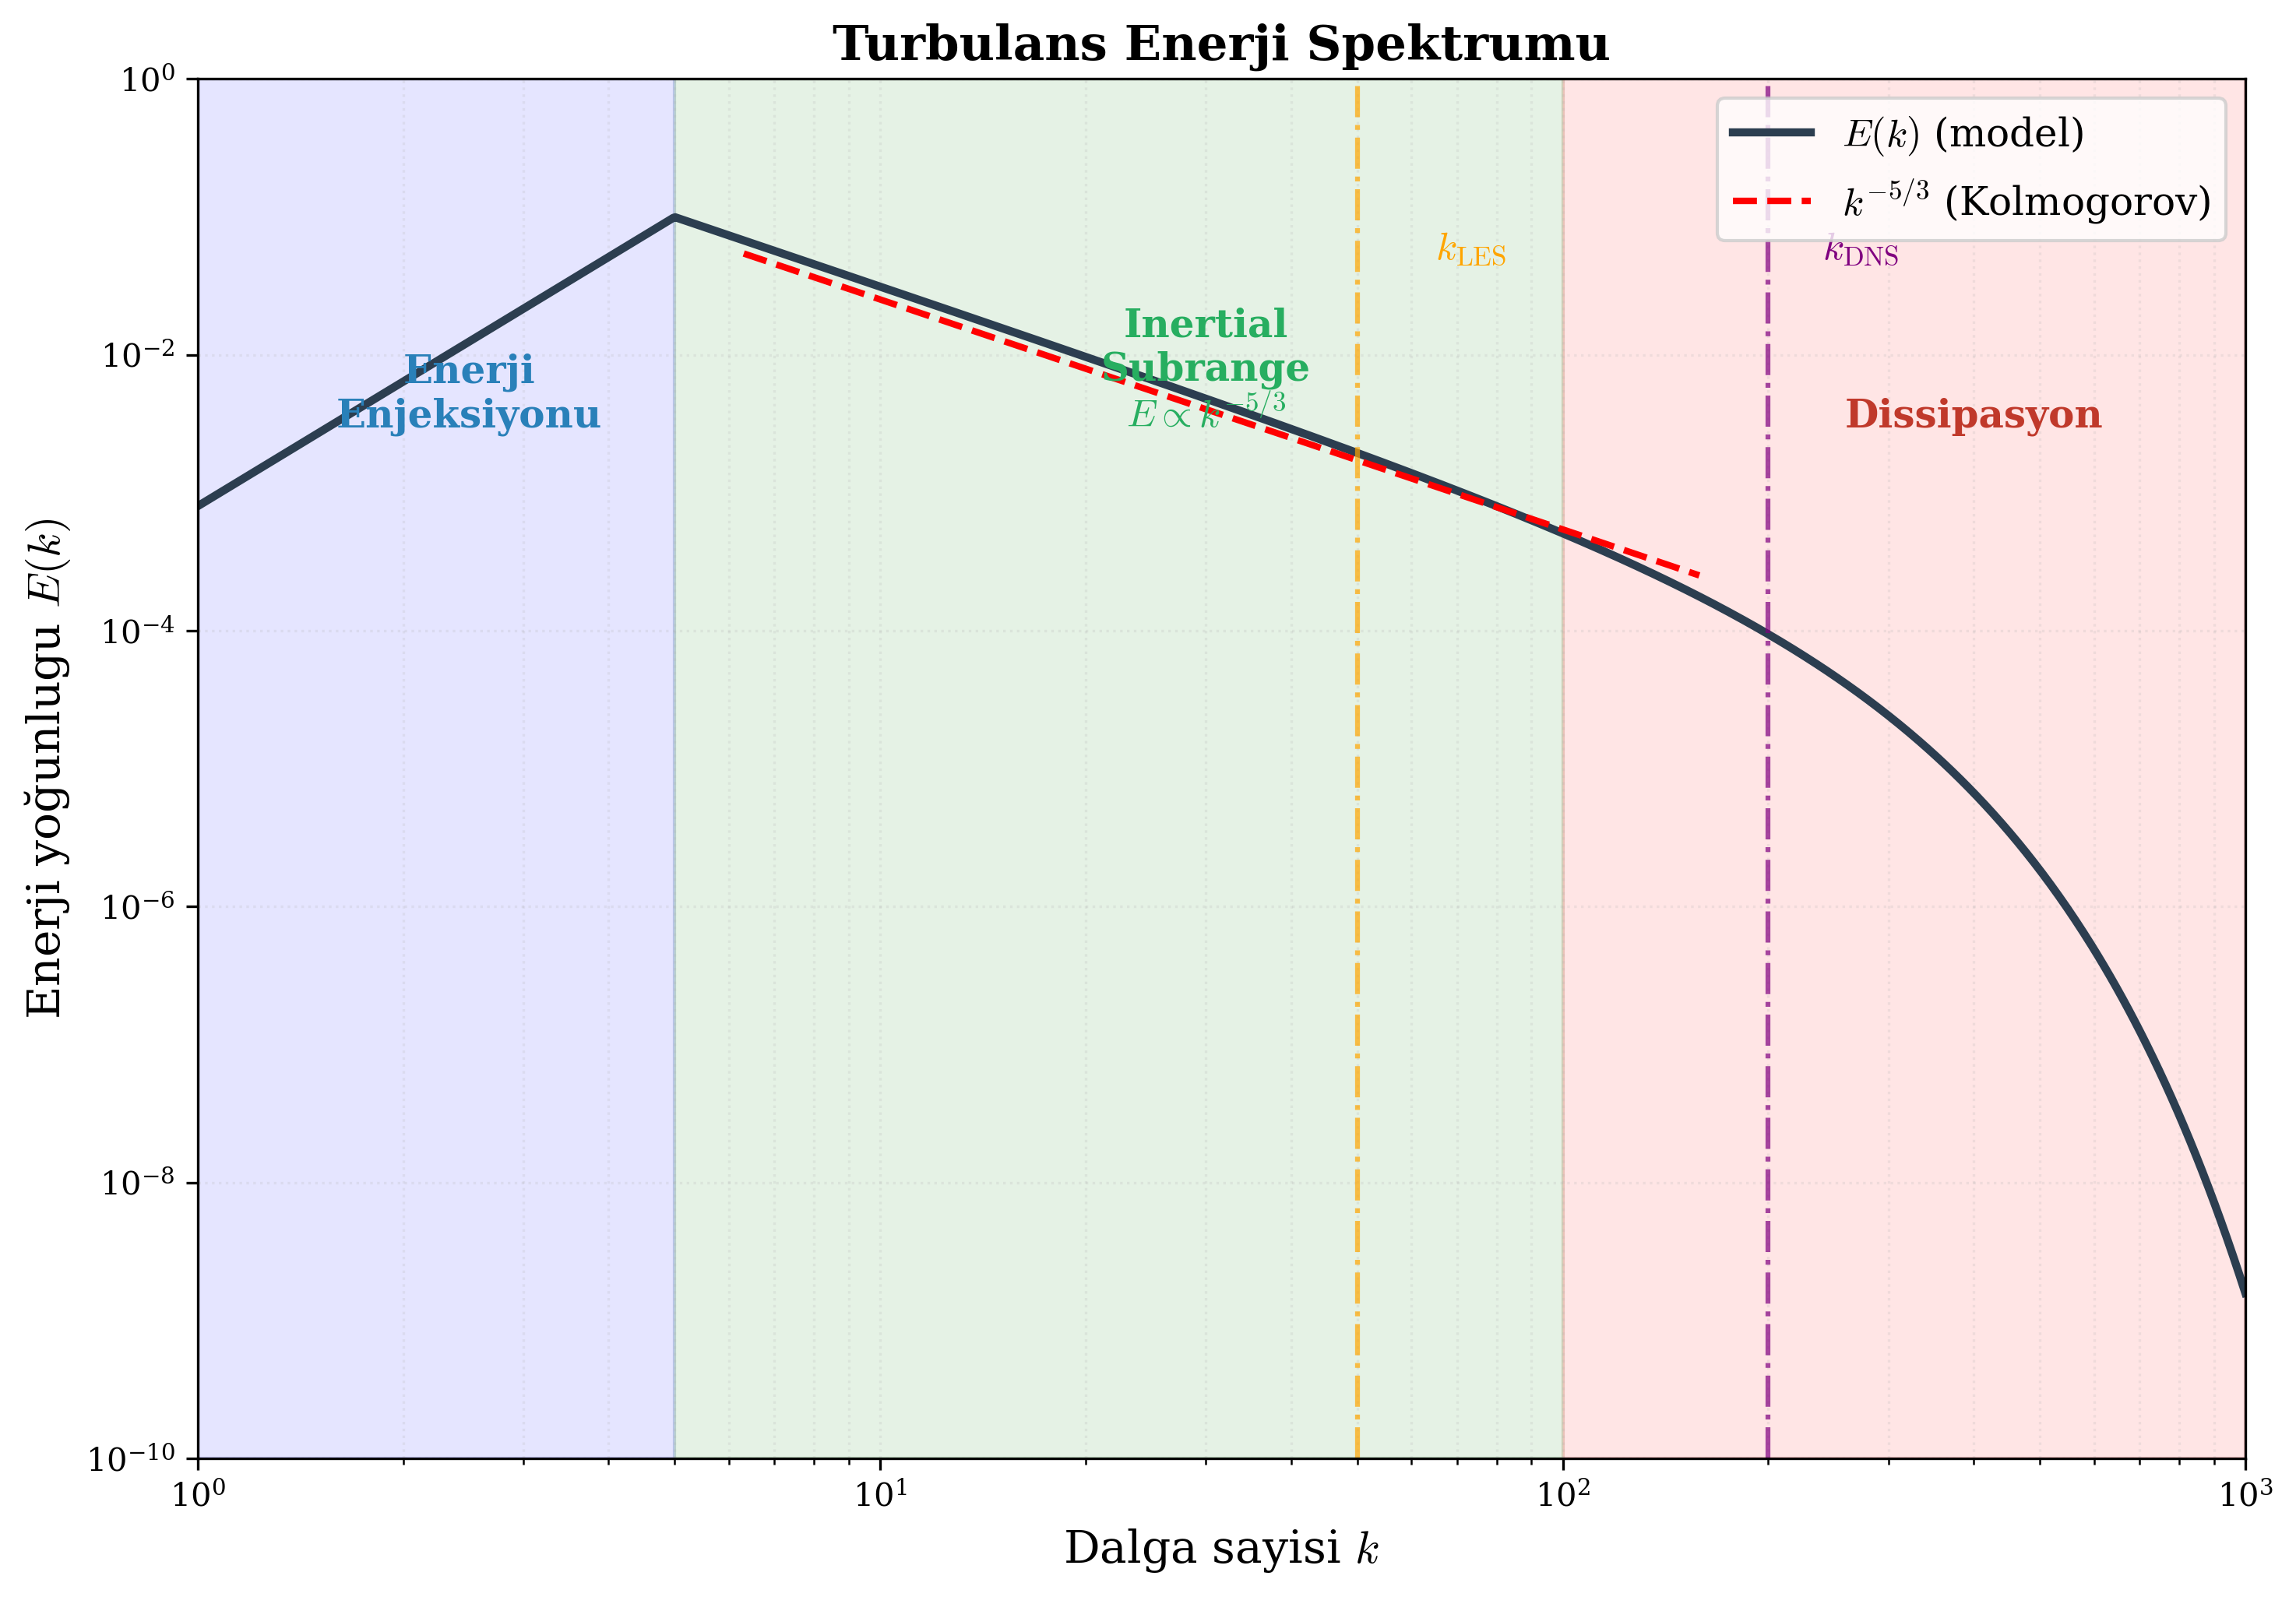
\includegraphics[width=0.85\textwidth]{energy_spectrum.png}
\caption{Türbülant enerji spektrumu $E(k)$. Üç bölge: enerji enjeksiyonu (düşük $k$), inertial subrange ($E(k) \sim k^{-5/3}$), ve dissipasyon (yüksek $k$). DNS tüm bölgeleri çözer; LES yalnızca kesme çizigisinin solunu çözer.}
\label{fig:energy_spectrum}
\end{figure}

% ============================================================
\section{Enerji Kaskadi}
\label{sec:cascade}

\subsection{Kavramsal Resim}

Türbülanstaki enerji ak\i{}s\i{} tek yönlüdür (3B'de):

\begin{equation}
\underbrace{\text{Enerji üretimi}}_{\text{büyük ölçek } (k \sim k_f)}
\quad\xrightarrow{\text{kaskad}}\quad
\underbrace{\text{Inertial transfer}}_{\text{orta ölçekler}}
\quad\xrightarrow{\text{kaskad}}\quad
\underbrace{\text{Dissipasyon}}_{\text{küçük ölçek } (k \sim k_\eta)}
\end{equation}

Detayli olarak üç bölge vardir:

\begin{enumerate}
\item \textbf{Energy-containing range} ($k \sim k_f$): D\i{}s forcing veya mean shear ile enerji enjekte edilir. Büyük girdaplar burada yasarlar. $E(k)$ davranisi forcing'e bağli (evrensel degil).

\item \textbf{Inertial subrange} ($k_f \ll k \ll k_\eta$): Enerji ne üretilir ne yok edilir, sadece büyük girdaplardan küçüklere \textbf{transfer} edilir. Kolmogorov $-5/3$ yasasi tam burada geçerlidir. Enerji transfer hizi sabittir: $\Pi(k) = \varepsilon$.

\item \textbf{Dissipation range} ($k \gtrsim k_\eta$): Viskoz kuvvetler baskindir. Kinetik enerji isiya donusur:
\begin{equation}
\varepsilon = 2\nu\,\mathcal{Z}, \qquad \mathcal{Z} = \frac{1}{2}\langle|\vect{\omega}|^2\rangle \;\text{(enstrofi)}
\label{eq:dissipation_enstrophy}
\end{equation}
\end{enumerate}

\begin{figure}[H]
\centering
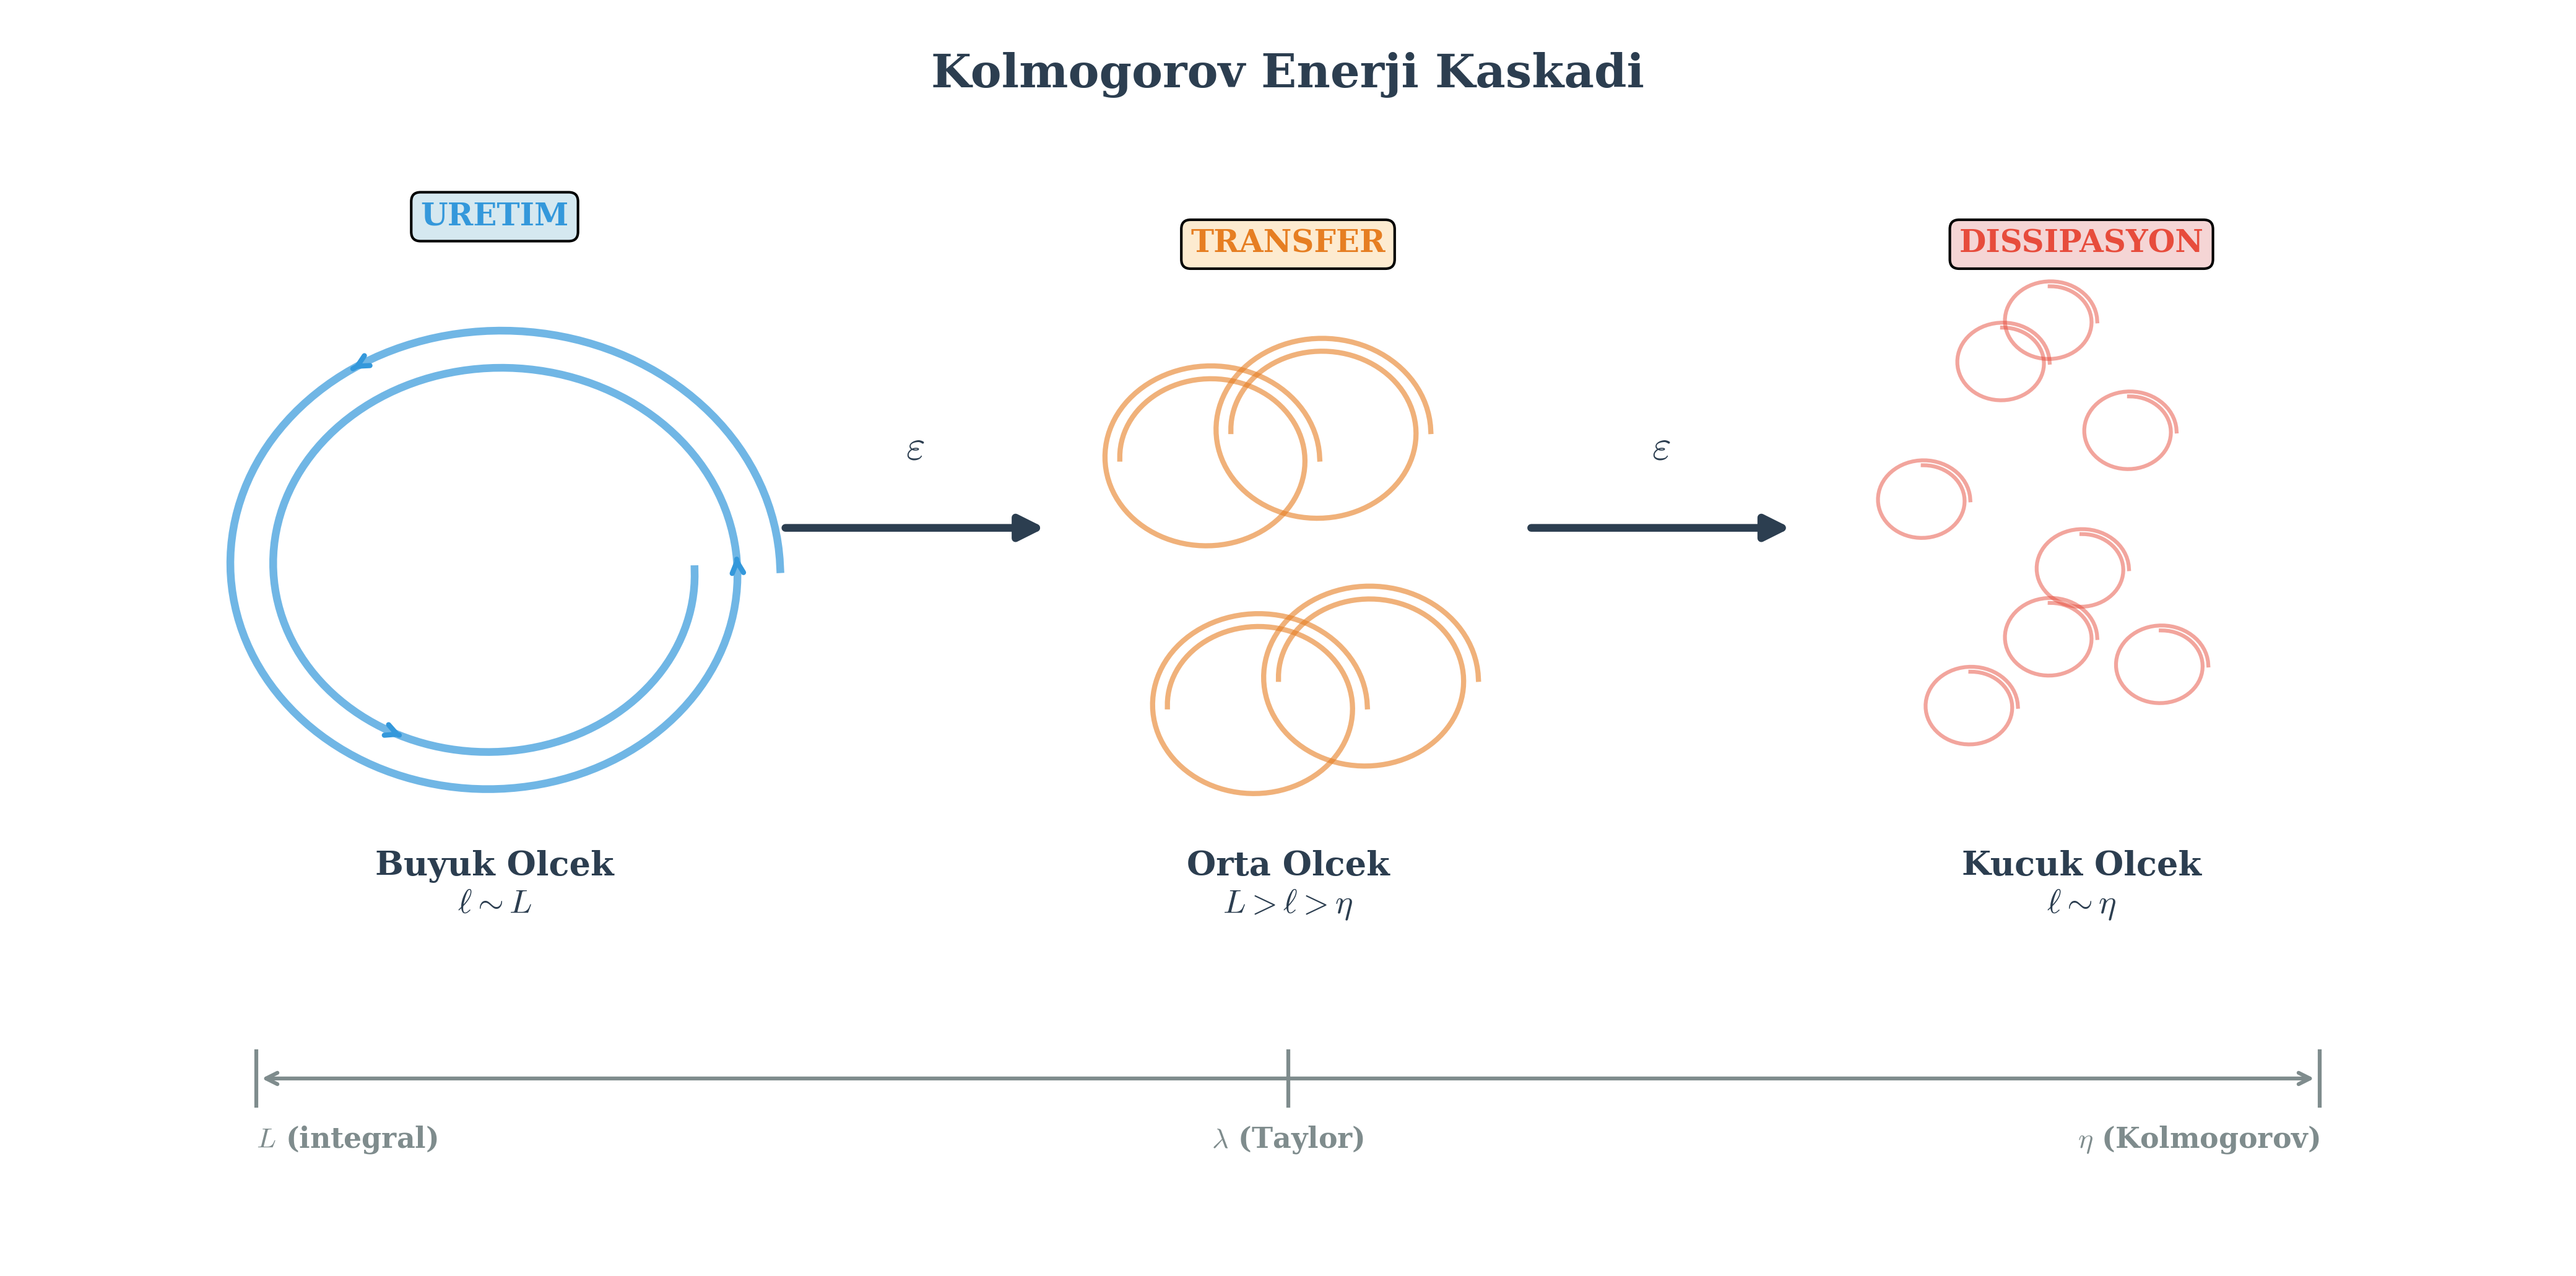
\includegraphics[width=0.8\textwidth]{energy_cascade.png}
\caption{Enerji kaskadı şematik gösterimi. Soldan sağa: enerji üretimi, inertial transfer ($-5/3$ yasası), ve dissipasyon.}
\label{fig:energy_cascade}
\end{figure}


% ============================================================
\section{Kolmogorov Uzunluk Ölçegi}
\label{sec:kolmogorov_scale}

En küçük girdabin boyutu ne kadardir? Dissipasyon bölgesinde iki mekanizma yarışır: inertial transfer ($\varepsilon$) ve visköz difüzyon ($\nu$). Boyut analizi ile:

\begin{equation}
\eta = \left(\frac{\nu^3}{\varepsilon}\right)^{1/4}
\label{eq:kolmogorov_eta}
\end{equation}

\begin{proof}[Türetme]
$\eta$ bir uzunluktur $[\text{m}]$, ve sadece $\nu\;[\text{m}^2/\text{s}]$ ile $\varepsilon\;[\text{m}^2/\text{s}^3]$'a bağlidir:
\begin{align}
[\eta] &= [\nu^\alpha\,\varepsilon^\beta] \notag \\
\text{m} &= (\text{m}^2\,\text{s}^{-1})^\alpha \cdot (\text{m}^2\,\text{s}^{-3})^\beta
\end{align}
Metre: $1 = 2\alpha + 2\beta$. Saniye: $0 = -\alpha - 3\beta$, yani $\alpha = -3\beta$. Birinci denklemde: $1 = -6\beta + 2\beta = -4\beta$, dolayisiyla $\beta = -1/4$, $\alpha = 3/4$.
\begin{equation}
\eta = \nu^{3/4}\,\varepsilon^{-1/4} = \left(\frac{\nu^3}{\varepsilon}\right)^{1/4} \quad\checkmark
\end{equation}
\end{proof}

\subsection{$\eta$ ve $\Rey$ İlişkisi}

Integral ölçek $L$ ve büyük ölçek hiz $U$ ile $\varepsilon \sim U^3/L$ (boyutsal tahmin). O zaman:
\begin{equation}
\frac{\eta}{L} \sim \left(\frac{\nu^3}{U^3/L}\right)^{1/4}\cdot\frac{1}{L} = \left(\frac{\nu}{UL}\right)^{3/4} = \Rey^{-3/4}
\label{eq:eta_over_L}
\end{equation}

\begin{equation}
\boxed{\frac{\eta}{L} \sim \Rey^{-3/4}}
\end{equation}

$\Rey$ arttıkça en küçük girdap hızla küçülür: ölçek ayrımı genişler.


% ============================================================
\section{DNS (Direct Numerical Simulation)}
\label{sec:dns}

\subsection{Temel Fikir}

DNS, Navier-Stokes denklemlerini \textbf{hiçbir model kullanmadan} dogrudan çözer. Tüm ölçekler --- $\eta$'dan $L$'ye kadar --- çözünür.

\subsection{Grid Gereksinimleri}

DNS gridinin $\eta$'yi çözümleyecek kadar ince olmasi gerekir: $\Delta x \lesssim \eta$. Bu durumda her yönde gerekli nokta sayisi:
\begin{equation}
N \sim \frac{L}{\eta} \sim \Rey^{3/4}
\end{equation}

3D'de toplam nokta sayisi:
\begin{equation}
\boxed{N_{\text{total}} = N^3 \sim \Rey^{9/4}}
\label{eq:dns_cost}
\end{equation}

\begin{example}
Say\i{}sal tahminler:
\begin{center}
\begin{tabular}{ccc}
\toprule
$\Rey$ & $N_{\text{total}} \sim \Rey^{9/4}$ & Durum \\
\midrule
$1{,}000$ & $\sim 5.6\times10^6$ & Masaustu bilgisayar \\
$3{,}000$ & $\sim 8.8\times10^7$ & İstasyon/kucuk cluster \\
$10{,}000$ & $\sim 5.6\times10^9$ & Süper bilgisayar \\
$100{,}000$ & $\sim 10^{12}$ & Dünyanin en buyuk bilgisayarlari \\
\bottomrule
\end{tabular}
\end{center}

$\Rey = 10{,}000$ için: $\eta / L \sim 10{,}000^{-3/4} \approx 10^{-3}$. Eğer $L = 10$ (bizim $L_y$) ise $\eta \approx 0.01$ ve grid $N \approx 1000$. 3D'de $10^9$ nokta. Her zaman adimi için 3D FFT: $\sim 10^{10}$ islem. Binlerce zaman adimi ile çarpilinca --- birkac gün süper bilgisayarda.
\end{example}

\subsection{Bizim DNS'imiz}

Projede DNS, \textbf{validasyon} için kullanilir (INNATE'in dogru sonuc verip vermedigini kontrol etmek için). DNS'i düsük $\Rey$'de yapariz:
\begin{itemize}
\item $\Rey = 1000$: Grid $\approx 192\times320\times128$ (yapılabilir)
\item $\Rey = 3000$: Grid $\approx 384\times640\times256$ (zorlayici ama mumkun)
\item $\Rey = 10000$: Grid $\approx 2048\times3200\times1280$ --- $\sim8.4$ milyar nokta, \textbf{imkansiz} (bizim kaynaklarla)
\end{itemize}

Yüksek $\Rey$'de INNATE, DNS yerine LES yaparak sonuc uretir. DNS sadece referans olarak dusuk $\Rey$'de kullanilir.


% ============================================================
\section{LES (Large Eddy Simulation)}
\label{sec:les}

\subsection{Temel Fikir}

DNS'in $\Rey^{9/4}$ maliyeti kaldirilamaz. LES'in cozumu:
\begin{quote}
Büyük girdaplari \textbf{dogrudan çöz}, küçük girdaplari \textbf{modelle}.
\end{quote}

Fiziksel gerekce: büyük girdaplar geometriye baglidir ve tahmin edilemez; küçük girdaplar ise (Kolmogorov'a gore) evrensel ve izotropiktir, dolayisiyla basit modellerle iyi temsil edilebilir.

\subsection{Filtreleme}

LES'te hız alanı bir \textbf{uzaysal filtre} ile ayrıştırılır:
\begin{equation}
\bar{u}_i(\vect{x},t) = \int G(\vect{x}-\vect{x}',\Delta)\,u_i(\vect{x}',t)\,d\vect{x}'
\label{eq:les_filter}
\end{equation}

Burada $G$ filtre fonksiyonu, $\Delta$ filtre genisligi (grid boyutu). Filtreleme:
\begin{itemize}
\item \textbf{Cozunen (resolved)} kisim: $\bar{u}_i$ --- büyük girdaplar
\item \textbf{Cozunmeyen (subgrid-scale, SGS)} kisim: $u'_i = u_i - \bar{u}_i$ --- kucuk girdaplar
\end{itemize}

\subsection{Filtrelenmis Navier-Stokes Denklemleri}

NS denklemlerini filtreleyelim. Sureklilik denklemi filtreleme ile degismez:
\begin{equation}
\pd{\bar{u}_i}{x_i} = 0
\end{equation}

Momentum denklemi:
\begin{equation}
\pd{\bar{u}_i}{t} + \pd{(\bar{u}_i\bar{u}_j)}{x_j} = -\frac{1}{\rho}\pd{\bar{p}}{x_i} + \nu\pdd{\bar{u}_i}{x_j} - \pd{\tau_{ij}^{\text{sgs}}}{x_j}
\label{eq:les_ns}
\end{equation}

Burada $\tau_{ij}^{\text{sgs}}$ \textbf{sub-grid scale (SGS) stres tensorudur}:
\begin{equation}
\tau_{ij}^{\text{sgs}} = \overline{u_i u_j} - \bar{u}_i\bar{u}_j
\label{eq:sgs_stress}
\end{equation}

Bu terim \textbf{bilinmiyor} --- cozunmeyen küçük olceklerin cozunen olceklere etkisini temsil eder. LES'in tum zorluğu bu terimi modellemektir.

\begin{remark}
SGS stresinin fiziksel anlami: küçük girdaplarin buyuk girdaplara uyguladiği ``sürtünme kuvveti''. Net etki: enerjiyi küçük olceklere transfer etmek (dissipasyon sağlamak).
\end{remark}


% ============================================================
\section{Smagorinsky Modeli}
\label{sec:smagorinsky}

En basit ve en yaygin SGS modeli, Smagorinsky (1963) tarafindan atmosfer modellemesi için önerilmiştir.

\subsection{Eddy Viscosity Hipotezi}

SGS stresinin, Boussinesq eddy-viscosity hipotezi ile modellenebileceği varsayilir:
\begin{equation}
\tau_{ij}^{\text{sgs}} - \frac{1}{3}\tau_{kk}^{\text{sgs}}\,\delta_{ij} = -2\nu_t\,\bar{S}_{ij}
\label{eq:eddy_viscosity}
\end{equation}

Burada $\nu_t$ \textbf{türbülans (eddy) viskozitesidir} --- molekuler viskoziteye ek olarak, küçük girdaplarin etkisini temsil eder. $\bar{S}_{ij}$ filtrelenmis strain rate tensoru:
\begin{equation}
\bar{S}_{ij} = \frac{1}{2}\left(\pd{\bar{u}_i}{x_j} + \pd{\bar{u}_j}{x_i}\right)
\label{eq:strain_rate}
\end{equation}

\subsection{Smagorinsky Formulasyonu}

$\nu_t$ boyut analizi ile belirlenir:
\begin{equation}
[\nu_t] = \text{m}^2/\text{s} = [\text{uzunluk}]^2 \cdot [\text{zaman}]^{-1}
\end{equation}

Elimizdeki uzunluk olcegi: filtre genisligi $\Delta$. Zaman olcegi: $1/|\bar{S}|$. Dolayisiyla:
\begin{equation}
\boxed{\nu_t = (C_s\,\Delta)^2\,|\bar{S}|}
\label{eq:smagorinsky}
\end{equation}

Burada:
\begin{itemize}
\item $C_s \approx 0.1\text{--}0.2$: \textbf{Smagorinsky sabiti} (boyutsuz)
\item $\Delta = (\Delta x\cdot\Delta y\cdot\Delta z)^{1/3}$: filtre genisligi (kup kok)
\item $|\bar{S}| = \sqrt{2\,\bar{S}_{ij}\bar{S}_{ij}}$: strain rate magnitude
\end{itemize}

\begin{remark}
$C_s$'nin degeri tartismalidir. Homojen izotropik turbulans icin $C_s \approx 0.17$ (Lilly, 1967'nin teorik tahmini). Kanal akisi icin $C_s \approx 0.1$ daha uygun. INNATE'te $C_s$ \textbf{ogrenilebilir bir parametredir} --- model, probleme ozgu optimal degeri kendi bulur.
\end{remark}

\subsection{Efektif Viskozite}

LES'te toplam viskoz etki:
\begin{equation}
\nu_{\text{eff}} = \nu + \nu_t
\label{eq:nu_eff}
\end{equation}

Filtrelenmis momentum denklemi:
\begin{equation}
\pd{\bar{u}_i}{t} + (\bar{\vect{u}}\cdot\gradient)\bar{u}_i = -\frac{1}{\rho}\pd{\bar{p}}{x_i} + \nu_{\text{eff}}\laplacian\bar{u}_i
\label{eq:les_effective}
\end{equation}

Bu form, DNS denkleminin \emph{aynısı}'dır --- tek fark $\nu$ yerine $\nu_{\text{eff}}$ kullanılması. Çok zarif: LES, DNS kodunun üzerine sadece $\nu_t$ hesabi eklenerek uygulanabilir.

\subsection{Strain Rate Magnitude Hesabi}

$|\bar{S}|$'yi acik olarak yazmak gerekirse (3D'de):

\begin{align}
\bar{S}_{ij}\bar{S}_{ij} &= \bar{S}_{xx}^2 + \bar{S}_{yy}^2 + \bar{S}_{zz}^2 + 2(\bar{S}_{xy}^2 + \bar{S}_{xz}^2 + \bar{S}_{yz}^2) \label{eq:sij_sij}
\end{align}

Her bilesen:
\begin{align}
\bar{S}_{xx} &= \pd{\bar{u}}{x}, \qquad \bar{S}_{yy} = \pd{\bar{v}}{y}, \qquad \bar{S}_{zz} = \pd{\bar{w}}{z} \\
\bar{S}_{xy} &= \frac{1}{2}\left(\pd{\bar{u}}{y}+\pd{\bar{v}}{x}\right), \quad
\bar{S}_{xz} = \frac{1}{2}\left(\pd{\bar{u}}{z}+\pd{\bar{w}}{x}\right), \quad
\bar{S}_{yz} = \frac{1}{2}\left(\pd{\bar{v}}{z}+\pd{\bar{w}}{y}\right)
\end{align}

\begin{equation}
|\bar{S}| = \sqrt{2\,\bar{S}_{ij}\bar{S}_{ij}}
\label{eq:strain_mag}
\end{equation}

Tüm bu türevler spectral yöntemle (Bölüm~\ref{ch:spectral}) hesaplanir.


% ============================================================
\section{INNATE'te EddyViscosity3D}
\label{sec:eddy_viscosity_innate}

Projemizdeki \texttt{EddyViscosity3D} noronu, Smagorinsky modelinin INNATE implementasyonudur.

\subsection{Noron Yapisi}

\begin{equation}
\nu_t = \big(\underbrace{\tilde{C}_s}_{\text{ogrenilebilir}}\cdot\Delta\big)^2 \cdot |\bar{S}|
\end{equation}

\textbf{Tek ogrenilebilir parametre:} $\tilde{C}_s$ (başlangıç değeri $0.15$, $[0.05, 0.30]$ arasinda clamp edilir).

\textbf{Grid spacing:}
\begin{equation}
\Delta = (\Delta x \cdot \Delta y \cdot \Delta z)^{1/3} = \left(\frac{L_x}{N_x}\cdot\frac{L_y}{N_y}\cdot\frac{L_z}{N_z}\right)^{1/3}
\end{equation}

Bizim grid icin: $\Delta = (6/96 \cdot 10/160 \cdot 4/64)^{1/3} = (0.0625 \cdot 0.0625 \cdot 0.0625)^{1/3} = 0.0625$.

\subsection{Neden LES Zorunlu?}

63 saatlik basarisiz egitimin \textbf{birincil sebebi} EddyViscosity3D'nin KAPALI olmasiydi. Grid analizi sonuclari bunu dogrular:

\begin{center}
\begin{tabular}{lcc}
\toprule
Grid & $\Rey = 5{,}000$ & $\Rey = 10{,}000$ \\
\midrule
$96\times160\times64$ (LES skoru) & 80/100 (iyi) & 74/100 (makul) \\
$32\times48\times24$ (LES skoru) & 60/100 (zayif) & 44/100 (yetersiz) \\
DNS gereksinimleri & $\sim10^8$ nokta & $\sim8.4\times10^9$ nokta \\
\bottomrule
\end{tabular}
\end{center}

$96\times160\times64 = 983{,}040$ nokta. $\Rey = 10{,}000$ için DNS $\sim 8.4\times10^9$ nokta gerektirir --- $8{,}500\times$ daha fazla. LES olmadan bu gridde yüksek $\Rey$ çözülemez: subgrid-scale dissipasyon saglanamaz ve enerji birikir $\to$ sayisal patlama (NaN).


% ============================================================
\section{LES Ötesinde: Gelismis SGS Modelleri}
\label{sec:advanced_sgs}

Smagorinsky modeli basit ve saglamdir ama sinirliliklari vardir:

\begin{itemize}
\item Duvar yakininda asiri dissipasyon verir ($C_s$'yi küçültmek gerekir).
\item Laminar--türbülant geçiste türbülans geçiş başlatamaz (``backscatter'' yoktur).
\item $C_s$ sabittir --- aslinda akisa ve konuma baglidir.
\end{itemize}

Gelismis modeller:
\begin{description}
\item[Dynamic Smagorinsky (Germano, 1991):] $C_s$'yi lokal olarak akinstan hesaplar (test filtre kullanarak). Cok basarili ama hesaplama maliyeti yüksek.
\item[WALE (Nicoud \& Ducros, 1999):] Duvar yakininda dogru asimptotik davranis. Ek turev hesabi gerektirir.
\item[Sigma model (Nicoud et al., 2011):] Hiz gradient tensorunun tekil degerleri ile $\nu_t$ hesaplar. Duvar yakininda ve laminar akista dogru sonuc verir.
\end{description}

\begin{remark}
INNATE'te $C_s$ zaten ogrenilebilir oldugundan, modelin Dynamic Smagorinsky'nin isini ``ogrenme yoluyla'' yapmasini bekliyoruz. Lokal-adaptif parametreler kullanilirsa (Yol~C mimarisi), $C_s(\vect{x},t)$ uzaysal olarak degisir --- bu, Dynamic Smagorinsky'ye fonksiyonel olarak esittir.
\end{remark}


% ============================================================
\section{Bu Bölümün Özeti}

\begin{enumerate}
\item \textbf{Türbülans}: Duzensiz, cok-olcekli, kaotik akis. $\Rey$ arttikca ortaya cikar.
\item \textbf{Kolmogorov teorisi}: Inertial subrange'de $E(k) = C_K\varepsilon^{2/3}k^{-5/3}$ (evrensel).
\item \textbf{Kolmogorov olcegi}: $\eta = (\nu^3/\varepsilon)^{1/4}$, $\eta/L \sim \Rey^{-3/4}$.
\item \textbf{DNS maliyeti}: $N^3 \sim \Rey^{9/4}$ --- yüksek $\Rey$'de imkansiz.
\item \textbf{LES}: Buyuk girdaplari coz, kucukleri modelle. SGS stresi: $\tau_{ij}^{\text{sgs}} = \overline{u_iu_j} - \bar{u}_i\bar{u}_j$.
\item \textbf{Smagorinsky}: $\nu_t = (C_s\Delta)^2|\bar{S}|$ --- basit, sağlam, ama sabit $C_s$.
\item \textbf{INNATE'te LES}: EddyViscosity3D noronu, ogrenilebilir $C_s$ ile Smagorinsky modeli uygular. Grid analizi: $96\times160\times64$ gridde $\Rey = 10{,}000$ için LES zorunlu.
\end{enumerate}

Bir sonraki bolumde, turbulans tahmini icin gelistirilen neural operator yaklasimlarini --- PINN, FNO, DeepONet ve bizim INNATE konseptimizi --- inceliyoruz.

\chapter{Neural Operators ve INNATE Konsepti}
\label{ch:neural_operators}

Bu bolumde, kismi diferansiyel denklem (PDE) cozumune makine ogrenmesi perspektifinden yaklasan yontemleri inceliyoruz. Geleneksel cozuculerden baslayarak, PINN ve FNO gibi guncel yaklasimlardan gecip, projemizin temelini olusturan INNATE konseptine ulasacagiz.


% ============================================================
\section{Geleneksel PDE Cozuculeri}
\label{sec:geleneksel}

\subsection{Mevcut Yontemler}

PDE cozumu icin dort ana sayisal yontem vardir:

\begin{description}
\item[FDM (Finite Difference Method):] Turevleri Taylor acilimi ile yaklasik hesaplar. Basit, ama yapisiz gridlerde zorluklu.
\item[FEM (Finite Element Method):] Zayif (weak) formda cozum. Karmasik geometrilere uyumlu. Yapisal mekanik ve isi transferinde baskın.
\item[FVM (Finite Volume Method):] Korunum denklemlerini hacim integrasyon ile cozer. CFD'de en yaygin (OpenFOAM, Fluent).
\item[Spectral:] Fourier/Chebyshev bazlarinda cozum. Üstel doğruluk ama sadece basit geometrilerde (Bolum~\ref{ch:spectral}).
\end{description}

\subsection{Ortak Sorun: Hesaplama Maliyeti}

Tum bu yontemlerin ortak siniri: \textbf{her parametre seti icin bastan cozum gerekir}.

$\Rey = 5000$'de mixed convection problemini cozdugunuzu dusunun. Sonra $\Rey = 5500$ icin istiyorsunuz --- tum hesaplamayi \textbf{sifirdan} tekrarlamaniz gerekir. Grid olustur, baslangic kosullarini ata, zaman adimlarini isle\ldots

\begin{equation}
\text{100 farkli parametre} \times \text{her biri 10 saat} = \text{1000 saat hesaplama}
\end{equation}

Tasarim optimizasyonu, belirsizlik analizi, parametre taramasi gibi uygulamalarda bu maliyet kaldirilamaz.


% ============================================================
\section{Veri-Gudumlu Yaklasimlar}
\label{sec:data_driven}

Makine ogrenmesinin vaat ettigi: \textbf{bir kere egit, sonra aninda tahmin et}.

\subsection{Saf Veri-Gudumlu Modeller}

En basit yaklasim: DNS verisinden bir sinir agi egit.
\begin{equation}
\text{Girdi: } (\Rey, \Ray, t, \vect{x}) \quad\xrightarrow{\text{NN}}\quad \text{Cikti: } (\vect{u}, p, T)
\end{equation}

\textbf{Avantajlar:}
\begin{itemize}
\item Inference cok hizli (millisaniyeler)
\item Herhangi bir parametreye genellestirebilir (teoride)
\end{itemize}

\textbf{Dezavantajlar:}
\begin{itemize}
\item \textbf{Fizik bilgisi yok}: Sureklilik, enerji korunumu, sinir kosullari ihlal edilebilir
\item \textbf{Genellestirme zayif}: Egitim dağılımının disinda (out-of-distribution) tahminler guvenilmez
\item \textbf{Veri ihtiyaci cok}: Yuzlerce/binlerce DNS simulasyonu gerekir
\item \textbf{Yorumlanabilirlik yok}: Model ne ogrendi, neden bu sonucu verdi bilinmez
\end{itemize}


% ============================================================
\section{PINN (Physics-Informed Neural Networks)}
\label{sec:pinn}

\subsection{Temel Fikir}

Raissi, Perdikaris ve Karniadakis (2019) tarafindan populerlestirilen PINN'ler, fizik bilgisini \textbf{loss fonksiyonuna} gömer.

Standart bir sinir agi $u_\theta(\vect{x}, t)$ fiziksel alanin yaklasik cozumudur. Egitim kaybi:

\begin{equation}
\mathcal{L} = \underbrace{\mathcal{L}_{\text{data}}}_{\text{veri uyumu}} + \lambda\underbrace{\mathcal{L}_{\text{physics}}}_{\text{fizik kisiitlari}}
\label{eq:pinn_loss}
\end{equation}

Navier-Stokes icin fizik kaybi:
\begin{equation}
\mathcal{L}_{\text{physics}} = \left\|\pd{\vect{u}}{t} + (\vect{u}\cdot\gradient)\vect{u} + \gradient p - \nu\laplacian\vect{u}\right\|^2 + \left\|\divergence\vect{u}\right\|^2
\label{eq:pinn_physics}
\end{equation}

\subsection{Calisma Prensibi}

\begin{enumerate}
\item Sinir agini rastgele $(\vect{x}, t)$ noktalarinda degerlendir.
\item Otomatik turev (autograd) ile $\partial u/\partial t$, $\partial u/\partial x$, \ldots hesapla.
\item PDE residualini hesapla --- bu sifir olmali.
\item Residual + veri uyumu kaybi ile ağı eğit.
\end{enumerate}

\subsection{Avantaj ve Dezavantajlar}

\textbf{Avantajlar:}
\begin{itemize}
\item Az veri ile calisir (fizik bilgisi veriyi tamamlar)
\item Ters problemler cozebilir (bilinmeyen parametreleri tahmin)
\item Grid-free: herhangi bir $(\vect{x},t)$ noktasinda degerlendirebilir
\end{itemize}

\textbf{Dezavantajlar:}
\begin{itemize}
\item \textbf{Yavas egitim}: Her adimda autograd ile turev hesabi pahali
\item \textbf{Her problem icin yeniden egit}: Parametreler degisince ($\Rey$, geometri, \ldots) yeni egitim
\item \textbf{Mesh-bagimlilik}: Collocation noktalarinin dağılımı sonucu etkiler
\item \textbf{Zor optimizasyon}: Fizik kaybi ile veri kaybi arasinda dengeleme (``stiff'' gradyanlar)
\item \textbf{Turbulansda basarisiz}: Kaotik akislarda loss landscape cok karmasik, egitim yakinsamaz
\end{itemize}


% ============================================================
\section{FNO (Fourier Neural Operator)}
\label{sec:fno}

\subsection{Temel Fikir}

Li et al. (2021), tamamen farkli bir bakis acisi sundu: \textbf{operatör öğrenme}. Fonksiyondan fonksiyona eşleme:
\begin{equation}
\mathcal{G}_\theta: a(\vect{x}) \mapsto u(\vect{x})
\end{equation}

Ornegin: baslangic kosulundan ($a = u_0$) belirli bir zamandaki cozume ($u = u(T)$) esleme.

\subsection{FNO Katmani}

Her FNO katmani su yapidadir:
\begin{equation}
v_{l+1}(\vect{x}) = \sigma\!\Big(\underbrace{W_l\cdot v_l(\vect{x})}_{\text{lokal (lineer)}} + \underbrace{\mathcal{K}_l(v_l)(\vect{x})}_{\text{global (Fourier)}}\Big)
\label{eq:fno_layer}
\end{equation}

Fourier integral operatoru $\mathcal{K}_l$:
\begin{equation}
\mathcal{K}_l(v)(\vect{x}) = \mathcal{F}^{-1}\!\Big[R_l(\vect{k})\cdot\mathcal{F}[v](\vect{k})\Big](\vect{x})
\label{eq:fno_kernel}
\end{equation}

Yani:
\begin{enumerate}
\item $v$'yi Fourier uzayina tasi (FFT).
\item $R_l(\vect{k})$ matrisi ile carp (ogrenilebilir, her dalga sayisi icin farkli).
\item Fiziksel uzaya geri don (IFFT).
\end{enumerate}

\textbf{Neden çalisir?} Konvolusyon teoremi: fiziksel uzayda konvolusyon $=$ Fourier uzayinda carpma. FNO, ogrenilmis bir integral kernel'i temsil eder.

\subsection{Avantaj ve Dezavantajlar}

\textbf{Avantajlar:}
\begin{itemize}
\item \textbf{Mesh-bagimsiz}: Farkli cozunurluklerde degerlendirebilir
\item \textbf{Hizli inference}: Bir kere egit, aninda tahmin et
\item \textbf{Iyi genellestirme}: Ayni mimari, farkli parametrelere genellesir
\end{itemize}

\textbf{Dezavantajlar:}
\begin{itemize}
\item \textbf{Kara kutu}: $R_l(\vect{k})$ matrisleri fiziksel anlam tasimaz
\item \textbf{Cok veri gerekir}: Yuzlerce/binlerce DNS simulasyonundan egitim verisi
\item \textbf{Fizik garanti yok}: $\divergence\vect{u} = 0$ saglanamaz, enerji korunmaz
\item \textbf{Yuksek parametre sayisi}: $\sim 10^6$ parametre --- overfitting riski
\end{itemize}


% ============================================================
\section{DeepONet}
\label{sec:deeponet}

\subsection{Temel Fikir}

Lu et al. (2021), universal approximation theorem'in operatorlere genellemesine dayanarak DeepONet'i onerdi.

\textbf{Yapii:} Iki ayri alt ag:
\begin{itemize}
\item \textbf{Branch network}: Girdi fonksiyonunu $a(x)$'i kodlar $\to$ $[b_1, \ldots, b_p]$
\item \textbf{Trunk network}: Sorgu noktasi $\vect{y}$'yi kodlar $\to$ $[t_1, \ldots, t_p]$
\end{itemize}

Cikti:
\begin{equation}
\mathcal{G}_\theta(a)(\vect{y}) = \sum_{k=1}^{p} b_k(a)\cdot t_k(\vect{y})
\label{eq:deeponet}
\end{equation}

\begin{remark}
DeepONet, FNO'dan konsept olarak daha genel (sadece Fourier bazina bagliml degil), ama pratikte FNO akiskanlar problemlerinde daha basarili olmustur.
\end{remark}


% ============================================================
\section{INNATE Konsepti}
\label{sec:innate}

\subsection{Motivasyon}

Yukaridaki yaklaşımların hepsinde ortak bir sorun var: \textbf{fizik bilgisi ya zayif (loss'ta) ya da yok (kara kutu)}. INNATE tamamen farkli bir yol izler.

\subsection{Temel Fikir}

\begin{quote}
\textit{Navier-Stokes denklemlerinin HER TERiMi bir noron olsun.\\
Aginn yapisi = sayisal cozum adimlari.\\
Ogrenilen parametreler = fiziksel katsayilar.}
\end{quote}

Bunu somutlastiralim. NS momentum denklemi:
\begin{equation}
\underbrace{\pd{\vect{u}}{t}}_{\text{zaman evrimi}} = \underbrace{-(\vect{u}\cdot\gradient)\vect{u}}_{\text{Advection3D}} + \underbrace{\nu\laplacian\vect{u}}_{\text{Diffusion}} + \underbrace{-\gradient p}_{\text{Projection3D}} + \underbrace{\vect{F}}_{\text{Forcing3D}} + \underbrace{g\beta(T-T_0)\hat{e}_y}_{\text{Buoyancy3D}}
\label{eq:innate_ns}
\end{equation}

Her terimi bir \texttt{nn.Module} olarak implemente ediyoruz:

\begin{description}
\item[Advection3D:] $-(\vect{u}\cdot\gradient)\vect{u}$ hesaplar. Spectral turevler kullanir. Ogrenilebilir parametre: \texttt{advection\_modulator} (adveksiyon gucunu ayarlar).

\item[Diffusion:] $\nu\laplacian\vect{u}$ hesaplar. Spectral Laplacian kullanir. Ogrenilebilir parametre: \texttt{diffusion\_scale} (efektif viskoziteyi ayarlar).

\item[Projection3D:] $\divergence\vect{u} = 0$ kisitini zorlar. Helmholtz ayrışması (Bolum~\ref{subsec:projection}) uygular. Ogrenilebilir parametre: \texttt{pressure\_scale} (projeksiyon agresifligini ayarlar).

\item[Forcing3D:] $\vect{F}$ dis kuvvetini uygular (Kolmogorov forcing). Ogrenilebilir parametreler: \texttt{amplitude}, forcing profil genligini ayarlar.

\item[Buoyancy3D:] $g\beta(T-T_0)\hat{e}_y$ termal kaldirma kuvveti. Ogrenilebilir parametre: \texttt{buoyancy\_strength}.

\item[EddyViscosity3D:] $\nu_t = (C_s\Delta)^2|\bar{S}|$ SGS modeli (Bolum~\ref{sec:eddy_viscosity_innate}). Ogrenilebilir parametre: $C_s$.

\item[ThermalDiffusion3D:] $\kappa\laplacian T$ termal difuzyon. Ogrenilebilir parametre: \texttt{kappa\_scale}.

\item[ThermalAdvection3D:] $-(\vect{u}\cdot\gradient)T$ termal adveksiyon. Parametresiz (saf operatör).
\end{description}

\subsection{Ag Yapisi = Zaman Adimi}

Bir INNATE forward pass'i, NS'nin bir zaman adimina karsilik gelir:

\begin{equation}
\vect{u}^{n+1} = \vect{u}^n + \Delta t\cdot\Big[\underbrace{\text{Adv}(\vect{u}^n)}_{\text{Advection3D}} + \underbrace{\text{Diff}(\vect{u}^n)}_{\text{Diffusion}} + \underbrace{\text{Force}}_{\text{Forcing3D}} + \underbrace{\text{Buoy}(T^n)}_{\text{Buoyancy3D}}\Big]
\label{eq:innate_step1}
\end{equation}
\begin{equation}
\vect{u}^{n+1} \leftarrow \underbrace{\text{Proj}(\vect{u}^{n+1})}_{\text{Projection3D}} \qquad\text{(divergence-free yap)}
\label{eq:innate_step2}
\end{equation}

Bu, standart bir \textbf{fractional step} (Chorin projection) yonteminin birebir neural network versiyonudur.

\subsection{Yorumlanabilirlik}

INNATE'in en guclu ozelligi: \textbf{her parametre fiziksel anlam tasir}.

\begin{table}[H]
\centering
\caption{INNATE öğrenilebilir parametreleri ve fiziksel anlamlari}
\label{tab:innate_params}
\begin{tabular}{llcc}
\toprule
\textbf{Noron} & \textbf{Parametre} & \textbf{Başlangıç} & \textbf{Fiziksel Anlam} \\
\midrule
Advection3D & \texttt{advection\_modulator} & 1.0 & Adveksiyon gucu \\
Diffusion & \texttt{diffusion\_scale} & 1.0 & $\nu_{\text{eff}}/\nu$ orani \\
Projection3D & \texttt{pressure\_scale} & 1.0 & Projeksiyon gucuu \\
Forcing3D & \texttt{amplitude} & 1.0 & Forcing genligi \\
Buoyancy3D & \texttt{buoyancy\_strength} & 1.0 & Kaldirma kuvveti gucu \\
EddyViscosity3D & \texttt{smagorinsky\_coeff} & 0.15 & Smagorinsky $C_s$ \\
ThermalDiffusion3D & \texttt{kappa\_scale} & 1.0 & Termal difuzivite orani \\
ThermalAdvection3D & (parametresiz) & --- & Saf operatör \\
\bottomrule
\end{tabular}
\end{table}

Toplam: \textbf{$\sim$10 parametre}. Bir FNO veya PINN'de $\sim10^6$ parametre varken, INNATE $10^4$--$10^5$ kat daha az parametreyle calisir.

\begin{remark}
$C_s = 0.18$ ogrendiyse, bunun fiziksel anlami var: ``bu grid ve bu $\Rey$ icin optimal Smagorinsky katsayisi 0.18'dir.'' Bir FNO'nun ogrendigi $R_l(\vect{k})$ matrisinden boyle bir yorum cikaramazsiniz.
\end{remark}


% ============================================================
\section{INNATE vs Digerleri}
\label{sec:comparison}

\begin{table}[H]
\centering
\caption{PDE cozum yontemlerinin karşılaştırması}
\label{tab:comparison}
\begin{tabular}{lcccc}
\toprule
\textbf{Ozellik} & \textbf{DNS} & \textbf{PINN} & \textbf{FNO} & \textbf{INNATE} \\
\midrule
Fizik bilgisi & Tam & Loss'ta & Yok & \textbf{Yapisal} \\
Parametre sayisi & -- & $\sim10^6$ & $\sim10^6$ & $\sim10^1$ \\
Yorumlanabilirlik & Tam & Dusuk & Cok dusuk & \textbf{Yuksek} \\
Egitim verisi & -- & Az & \textbf{Cok} & Yok \\
Inference hizi & Yavas & Orta & Hizli & \textbf{Hizli} \\
Genellestirme & Yok & Sinirli & Iyi & Iyi \\
$\divergence\vect{u}=0$ & Tam & Yaklasik & Yok & \textbf{Tam} \\
Enerji korunumu & Tam & Yaklasik & Yok & \textbf{Yapisal} \\
\bottomrule
\end{tabular}
\end{table}

\subsection{Kritik Farklar}

\begin{enumerate}
\item \textbf{Fizik bilgisinin yeri:}
\begin{itemize}
\item PINN: Fizik, loss fonksiyonunda (``\textit{cezalandir}'')
\item FNO: Fizik yok, tamamen veriden ogren
\item INNATE: Fizik, ag yapisinda (``\textit{yapisal olarak zorla}'')
\end{itemize}

Ornek: $\divergence\vect{u} = 0$. PINN bunu loss'a ekler, ama tam olarak saglanamaz. FNO bu kisiti hiç bilmez. INNATE'te Projection3D noronu \textbf{her zaman adiminda} divergence-free projeksiyon uygular --- matematiksel olarak garanti.

\item \textbf{Parametre sayisi ve overfitting:}

$10^6$ parametreli bir FNO'yu egitmek icin binlerce DNS simulasyonu gerekir (yoksa overfitting). INNATE'te $\sim10$ fiziksel parametre var --- overfitting riski ihmal edilebilir. Hatta veriye bile ihtiyac yok (physics-only training).

\item \textbf{Genellestirme mekanizmasi:}

FNO: ``Yeterince veri görürse, yeni parametreleri de iyi tahmin eder'' (istatistiksel genellestirme).
INNATE: ``NS denklemleri zaten dogru, sadece katsayilari kalibre et'' (fiziksel genellestirme). Bu ikinci yaklasim çok daha guvenilirdir.
\end{enumerate}


% ============================================================
\section{Physics-Only Training}
\label{sec:physics_only}

INNATE'in en şasirtici ozelligi: \textbf{DNS verisi kullanilmadan eğitilebilir}.

\subsection{Nasil Mumkun?}

INNATE'in forward pass'i zaten NS'yi yapisal olarak cozer. Eger noron parametreleri doğru kalibre edilmişse, cikti fiziksel olarak dogru olacaktir. Parametreleri kalibre etmek icin DNS \emph{verisi} degil, \textbf{fiziksel kisitlar} yeterlidir:

\begin{align}
\mathcal{L}_{\text{total}} &= w_1\,\mathcal{L}_{\text{div}} + w_2\,\mathcal{L}_{\text{energy}} + w_3\,\mathcal{L}_{\text{spectrum}} + \cdots \label{eq:physics_loss}
\end{align}

Ornek fiziksel kisitlar:
\begin{itemize}
\item $\mathcal{L}_{\text{div}} = \|\divergence\vect{u}\|^2$: Sureklilik denklemi
\item $\mathcal{L}_{\text{energy}}$: Kinetik enerjinin fiziksel sinirlar icinde kalmasi
\item $\mathcal{L}_{\text{spectrum}}$: Enerji spektrumunun $-5/3$ yasasina uymasi
\item $\mathcal{L}_{\text{Nusselt}}$: Nusselt sayisinin fiziksel degerlerle uyumu
\end{itemize}

\subsection{DNS'in Rolu}

DNS verisi egitimde kullanilmaz. DNS sadece \textbf{validasyon} icindir: ``INNATE'in urettigi sonuc, DNS sonucu ile ne kadar uyumlu?''

Bu, bilimsel yontemin temelidir:
\begin{itemize}
\item \textbf{Teori} (INNATE yapisi = NS denklemleri)
\item \textbf{Kalibrasyon} (physics-only training = parametre ayari)
\item \textbf{Dogrulama} (DNS karsilastirmasi = deneysel test)
\end{itemize}


% ============================================================
\section{INNATE'in Mimari Evrimi}
\label{sec:mimari_evrim}

\subsection{Ilk Versiyon: PINN-INNATE Hibrit}

Projenin ilk versiyonunda her INNATE katmanina bir MLP (PhysicsModulator) eklenmisti:
\begin{equation}
\text{Scale} = \text{MLP}(E, \mathcal{Z}, \|\divergence\vect{u}\|, t) \qquad\text{(6 girdi} \to \text{3 cikti)}
\end{equation}

Bu hibrit yaklasimda:
\begin{itemize}
\item Toplam $10{,}144$ parametre
\item Bunun $10{,}116$'si (\%99.7) MLP'de
\item Sadece $28$'i INNATE noronlarinda
\end{itemize}

\subsection{63 Saatlik Başarısızlık}

Hibrit modelin 63 saatlik egitimi basarisiz oldu. Sebepleri:
\begin{enumerate}
\item \textbf{EddyViscosity3D KAPALI}: Grid-scale dissipasyon yok $\to$ enerji birikimi $\to$ patlama
\item \textbf{MLP fizigin yerine gecmeye calisiyor}: 6 global skalerden 3 scale faktörü ogrenmeye calismak --- kara kutu
\item \textbf{Yanlis loss tasarimi}: Nusselt loss'ta $\text{relu}(1-\text{Nu})^2$ kullanildi $\to$ $\text{Nu}\geq1$ olunca gradyan sifir
\item \textbf{Stabilite loss'u turbulansi engelliyor}: $\text{relu}(\mathcal{Z}/\mathcal{Z}_\text{ref}-10)^2$ $\to$ enstrofi artisini cezalandirir
\end{enumerate}

\subsection{Yeni Mimari: Saf INNATE}

Kritik karar (2026-02-18): \textbf{MLP'ler kaldirilacak}.

Yeni prensip:
\begin{quote}
INNATE noronlari, bir sinir agindaki noronlar \textbf{gibi} dusunulmeli.
Bir tane Advection3D degil, \textbf{yuzlerce} Advection3D noronu kullanilacak.
Her noronun kendi fiziksel parametreleri var.
Noronlarin ag yapisi, problemi ogreniyor --- MLP'ye gerek yok.
\end{quote}

\begin{equation}
\underbrace{\text{12 katman} \times (1\;\text{fizik noron} + 1\;\text{MLP}[843\;\text{param}])}_{\text{YANLIS: hibrit}}
\quad\neq\quad
\underbrace{\text{Yuzlerce fizik noronu} \to \text{ag olusturur}}_{\text{DOGRU: saf INNATE}}
\end{equation}

Bu yeni mimaride:
\begin{itemize}
\item Her noron 1--3 parametre tasir
\item Toplam binlerce parametre (hepsi fizik tabanli)
\item MLP sifir --- tamamen yorumlanabilir
\item LES (EddyViscosity3D) ACIK --- grid analizi bunu zorunlu kildi
\end{itemize}


% ============================================================
\section{Bu Bolumun Ozeti}

\begin{enumerate}
\item \textbf{Geleneksel cozuculer}: Her parametre icin yeniden coz --- pahali.
\item \textbf{PINN}: Fizigi loss'a gom, ama yavas ve turbulansda basarisiz.
\item \textbf{FNO}: Fourier uzayinda ogren, hizli ama kara kutu ve cok veri gerek.
\item \textbf{DeepONet}: Branch+Trunk yapisi, operator ogrenme.
\item \textbf{INNATE}: NS'nin her terimi bir noron. Yapisal fizik, $\sim10$ ogrenilebilir parametre, physics-only training.
\item \textbf{Karsilastirma}: INNATE, yorumlanabilirlik ve fizik garantisi acisindan diger yontemlerden ustun.
\item \textbf{Physics-only training}: DNS verisi kullanilmadan, fiziksel kisitlarla kalibre edilir.
\item \textbf{MLP'siz saf INNATE}: 63 saatlik basarisizliktan alinan ders --- fizik noronlari ag olusturur, kara kutu MLP gereksiz.
\end{enumerate}

Sonraki bolumlerde, bu konseptin somut uygulamasini --- bizim 3D mixed convection problemimizi (Bolum~\ref{ch:bizim_problem}) ve INNATE mimarisinin detaylarini (Bolum~\ref{ch:innate_mimari}) --- inceleyecegiz.


% KISIM II — PROBLEM VE MİMARİ
% ============================================================
% Bölüm 8: Bizim Problemimiz -- 3D Mixed Convection
% ============================================================

\chapter{Bizim Problemimiz: 3D Mixed Convection}
\label{ch:bizim_problem}

\"Onceki bölümlerde teorik temelleri kurduk: Navier--Stokes denklemleri, Boussinesq yaklaşımı, spektral yöntemler, türbülans ve LES, neural operator kavramları. Şimdi bu bilgilerin tamamını somut bir probleme uyguluyoruz.

Bu bölüm, projenin fiziksel çerçevesini eksiksiz tanımlar: geometri, sınır koşulları, zorlama mekanizması, sıcaklık ayrıştırması, boyutsuz denklemler, parametre uzayı, CFL analizi ve başlangıç koşulları.


% ============================================================
\section{Problem Tanımı ve Geometri}
\label{sec:problem_tanim}

\subsection{Domain}

Çözüm alanı, üç boyutlu dikdörtgen bir kutudur:
\begin{equation}
    \Omega = [0, L_x] \times [0, L_y] \times [0, L_z], \quad
    L_x = 6, \quad L_y = 10, \quad L_z = 4.
    \label{eq:domain}
\end{equation}
Burada $y$-ekseni dikey (yerçekimi yönü), $x$-ekseni akışın birincil yönü ve $z$-ekseni enine (spanwise) yöndür. Tüm uzunluklar boyutsuzdır; referans uzunluk $H$ alınmıştır.

Domain'in en-boy oranları $L_x : L_y : L_z = 3:5:2$ olarak seçilmiştir. Dikey boyutun ($L_y = 10$) büyük seçilmesinin nedeni: kaldırma kuvveti kaynaklı büyük ölçekli konveksiyon hücrelerinin (plume) yeterli alan bulmasıdır. Yatay boyutlar ($L_x = 6$, $L_z = 4$) ise Kolmogorov forcing'in yeterli sayıda dalga boyunu barındırması ve spanwise yapıların gelişebilmesi için uygundur.

\subsection{Sınır Koşulları}

\textbf{Tüm yönlerde periyodik:}
\begin{equation}
    \vect{u}(0, y, z, t) = \vect{u}(L_x, y, z, t), \quad
    \vect{u}(x, y, 0, t) = \vect{u}(x, y, L_z, t), \quad
    \vect{u}(x, 0, z, t) = \vect{u}(x, L_y, z, t).
    \label{eq:periodic_bc}
\end{equation}
Bu tamamen periyodik yapı, FFT tabanlı spektral yöntemlerin doğrudan uygulanmasına olanak tanır: türevler, Poisson çözücü ve dealiasing işlemleri Fourier uzayında analitik olarak yapılır.

\textbf{Sıcaklık koşulları:}
\begin{itemize}
    \item Alt yüzey ($y = 0$): sıcak, $T = T_{\text{hot}} = 20\,^{\circ}\mathrm{C}$
    \item Üst yüzey ($y = L_y$): soğuk, $T = T_{\text{cold}} = 0\,^{\circ}\mathrm{C}$
    \item Sıcaklık farkı: $\Delta T = T_{\text{hot}} - T_{\text{cold}} = 20\,^{\circ}\mathrm{C}$
\end{itemize}
Bu sıcaklık koşulu, Rayleigh--B\'{e}nard konveksiyonunun sürücüsüdür. Alttaki sıcak akışkan hafifleyerek yükselir, üstteki soğuk akışkan ağırlaşarak alçalır; bu dengesizlik konvektif hücrelere yol açar.

\begin{remark}
Alt sıcak, üst soğuk koşulu ile periyodik sınır koşulu arasında ciddi bir çelişki vardır. Bu çelişki ve çözümü Bölüm~\ref{sec:sicaklik_ayristirma}'da ele alınmaktadır.
\end{remark}

\subsection{Fiziksel Senaryo}

Bu problem, aşağıdaki gerçekçi senaryoları modeller:
\begin{itemize}
    \item \textbf{Dikey atrium:} Çok katlı bir binanın ortasındaki açık hacim. Taban ısıtılmış (yer ısıtma), tavan soğuk; aynı zamanda kapı/pencere açıklıklarından yatay rüzgâr girer.
    \item \textbf{Açık alan:} Güneş'ten ısınan zemin üzerinde, yatay rüzgârın etkisi altında oluşan atmosferik sınır tabaka.
    \item \textbf{Bina aralarındaki rüzgâr koridoru:} Binalar arasında kanallanmış rüzgâr ve zeminle bina yüzeyleri arasındaki sıcaklık farkının örneği.
\end{itemize}

%\begin{figure}[H]
%    \centering
%    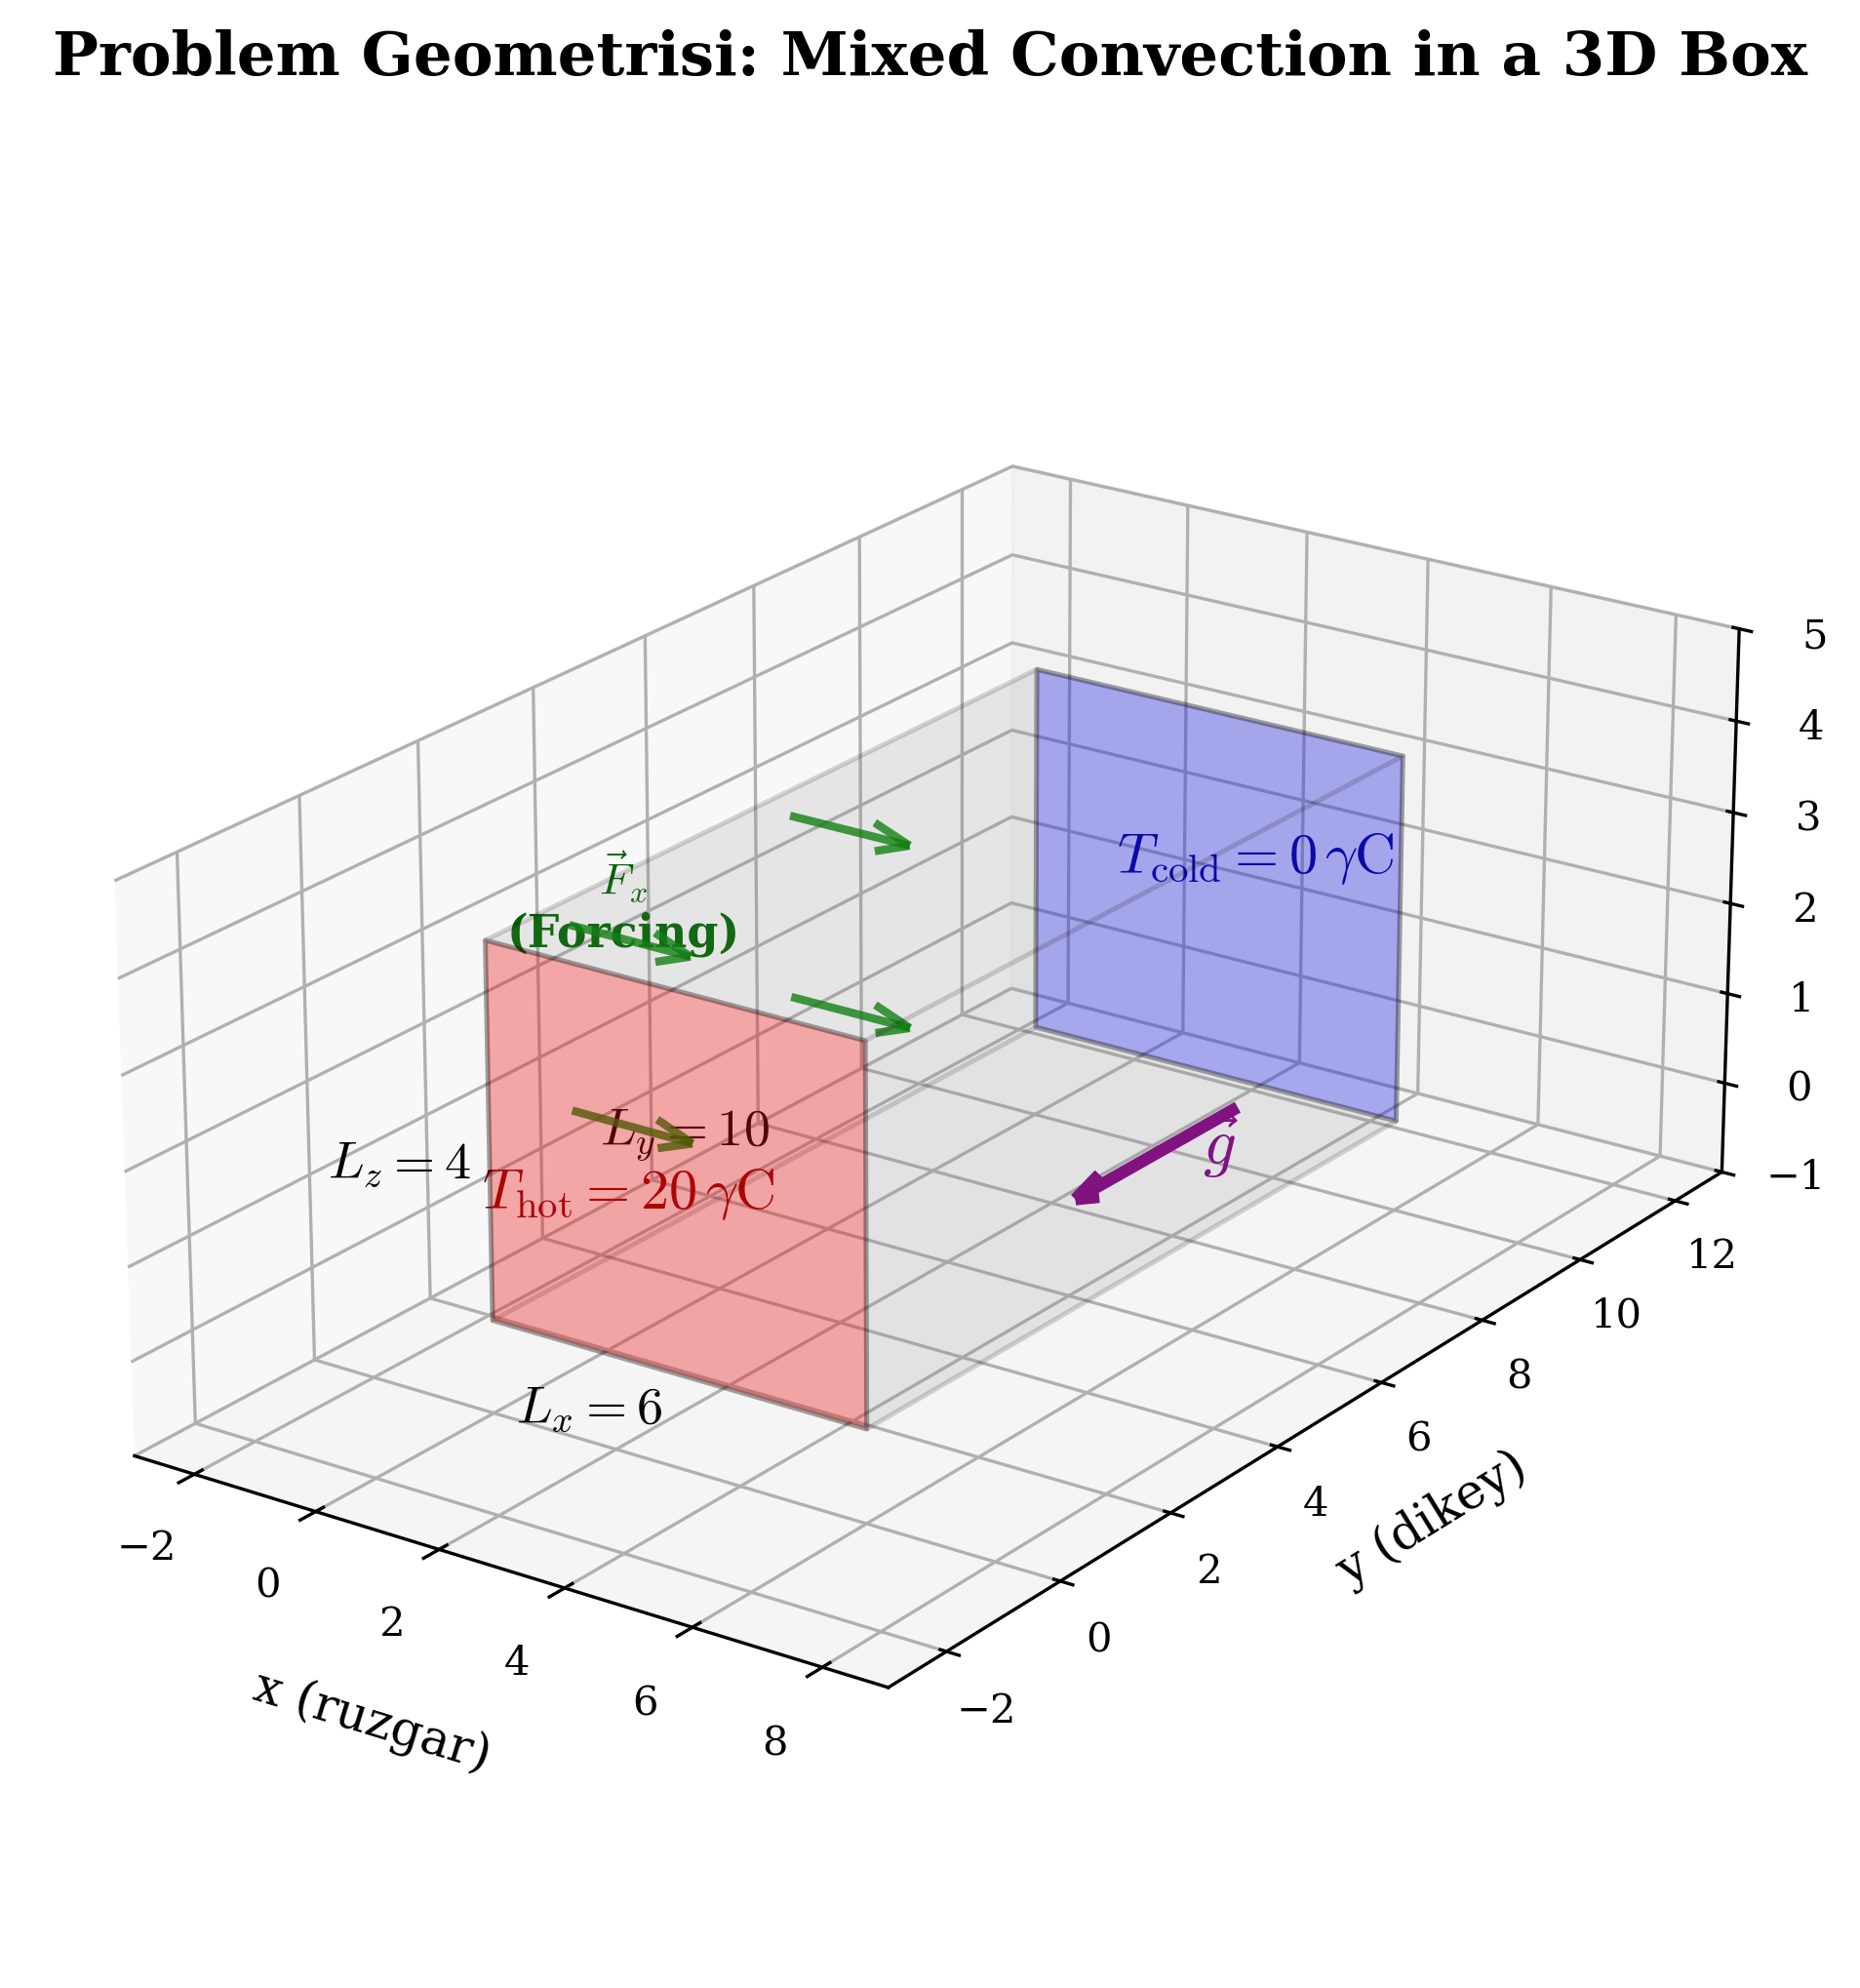
\includegraphics[width=0.85\textwidth]{problem_geometry.png}
%    \caption{3D mixed convection domain geometrisi. $L_x \times L_y \times L_z = 6 \times 10 \times 4$ boyutlu periyodik kutu. Alt yüzey sıcak ($T_{\text{hot}}$), üst yüzey soğuk ($T_{\text{cold}}$). Yatay ok, Kolmogorov forcing'in yönünü gösterir.}
%    \label{fig:problem_geometry}
%\end{figure}


% ============================================================
\section{Kolmogorov Forcing}
\label{sec:kolmogorov_forcing}

\subsection{Formülasyon}

Hız alanına uygulanan dış kütle kuvveti (body forcing):
\begin{equation}
    \vect{F}(y) = A \sin\!\left(\frac{k_f \cdot 2\pi y}{L_y}\right) \hat{\vect{e}}_x
    \label{eq:kolmogorov_forcing}
\end{equation}
\begin{itemize}
    \item $A$: genlik (öğrenilebilir parametre, INNATE'te)
    \item $k_f = 1$: zorlama dalga sayısı (tek mod)
    \item $\hat{\vect{e}}_x$: kuvvet $x$-yönündedir
    \item Kuvvet yalnızca $y$'ye bağlıdır: dikey konuma göre farklı şiddette rüzgâr
\end{itemize}

$k_f = 1$ seçimi, domain içinde tek bir sinüs dalgası anlımına gelir: $y = L_y/4$'te kuvvet pozitif ($+x$), $y = 3L_y/4$'te negatif ($-x$). Bu da bir kesme (shear) akışı yaratır.

\subsection{Neden Kolmogorov Forcing?}

Kolmogorov akışı (Kolmogorov flow), türbülans araştırmalarında standart bir benchmark'tir. Seçim nedenleri:

\begin{enumerate}
    \item \textbf{Analitik laminer çözüm:} Düşük $\Rey$ değerlerinde, karılı durum çözümü:
    \begin{equation}
        u_{\text{laminar}}(y) = \frac{A \, \Rey}{(k_f \cdot 2\pi / L_y)^2} \sin\!\left(\frac{k_f \cdot 2\pi y}{L_y}\right)
        \label{eq:kolmogorov_laminar}
    \end{equation}
    Bu analitik çözüm, kodun doğrulanması için vazgeçilmezdir.

    \item \textbf{Periyodik yapıya uyum:} Forcing fonksiyonu doğal olarak periyodiktir, FFT ile tam uyum içindedir.

    \item \textbf{Akademik standart:} Kolmogorov-type forcing, $\Rey$ aşıldığında türbülansa geçişi temiz biçimde üretir. Energy injection rate iyi tanımlıdır: $\varepsilon_{\text{input}} = \langle \vect{u} \cdot \vect{F} \rangle$.

    \item \textbf{Kontrol edilebilir rejim:} $A$ ayarlanarak, zorlanmış konveksiyon şiddeti sürekli değiştirilebilir.
\end{enumerate}

\subsection{Stochastic Mod: Ornstein--Uhlenbeck Süreci}

Gerçek rüzgâr sabit değildir; zamanla dalgalanır. Bu davranışı modellemek için genlik $A(t)$ bir Ornstein--Uhlenbeck (OU) sürecine bağlanır:
\begin{equation}
    dA = -\frac{A - A_0}{\tau_{\text{OU}}} \, dt + \sigma_{\text{OU}} \, dW(t)
    \label{eq:ou_process}
\end{equation}
\begin{itemize}
    \item $A_0$: ortalama genlik (mean reversion hedefi)
    \item $\tau_{\text{OU}}$: korelasyon zamanı (büyük $\to$ yavaş değişim)
    \item $\sigma_{\text{OU}}$: dalgalanma şiddeti
    \item $dW(t)$: Wiener süreci (Brownian motion)
\end{itemize}
OU süreci, sıfıra değil $A_0$'a dönme eğilimindedir; dolayısıyla rüzgâr hiçbir zaman ``ölmez'' ama gerçekçi şekilde dalgalanır. $k_f = 1$ seçimi ile bu mod, büyük ölçekli atmosferik rüzgâr dalgalanmasının basit bir surrogat'ıdır.

%\begin{figure}[H]
%    \centering
%    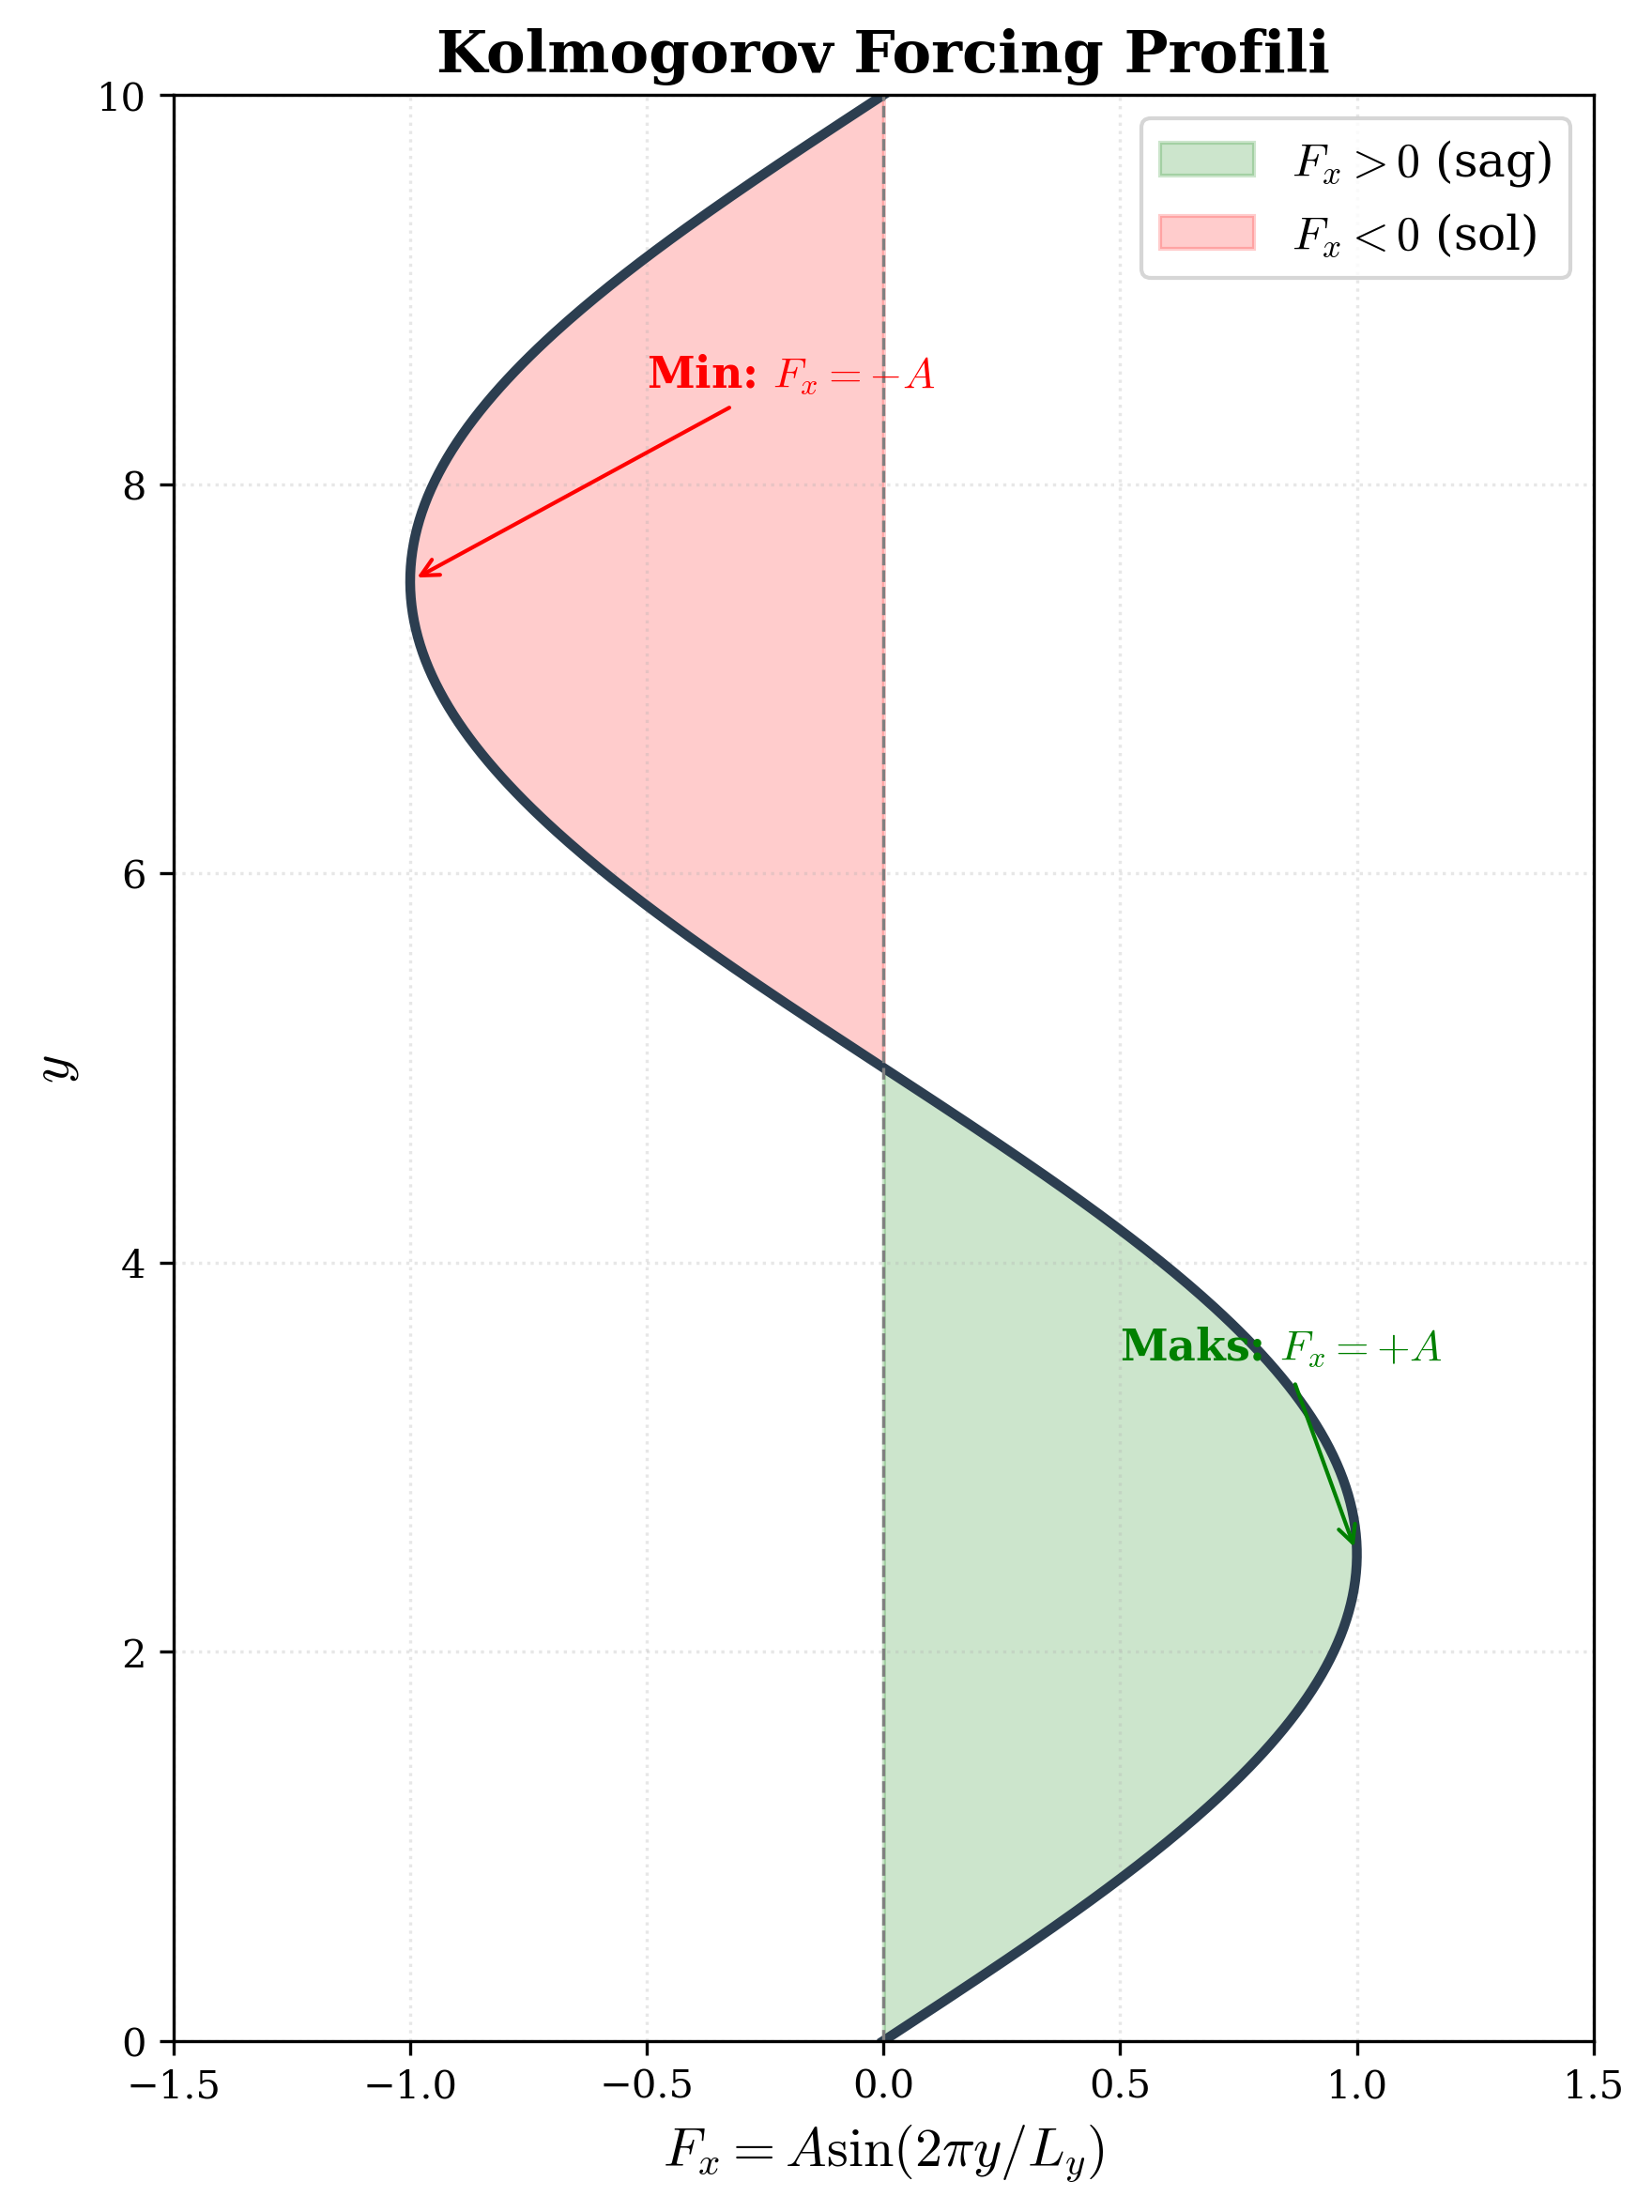
\includegraphics[width=0.80\textwidth]{kolmogorov_forcing.png}
%    \caption{Kolmogorov forcing profili. Sol: $F_x(y) = A\sin(2\pi y / L_y)$. Sağ: Stochastic modda genlik $A(t)$'nin OU süreci ile zamansal evrimi.}
%    \label{fig:kolmogorov_forcing}
%\end{figure}


% ============================================================
\section{Sıcaklık Ayrıştırması}
\label{sec:sicaklik_ayristirma}

Bu kısım, projenin teknik olarak en kritik noktalarından biridir. Periyodik sınır koşulları ile inhomogen sıcaklık koşulunu bağdaştırmak için sıcaklık alanının \textit{ayrıştırılması} gerekir.

\subsection{Sorun: Periyodik BC ile Sıcaklık Çelişkisi}

Periyodik sınır koşulu, $y$-yönünde şunu zorunlu kılar:
\begin{equation}
    T(x, 0, z, t) = T(x, L_y, z, t).
    \label{eq:periodic_T}
\end{equation}
Ancak fiziksel problemde:
\begin{equation}
    T(x, 0, z, t) = T_{\text{hot}} = 20\,^{\circ}\mathrm{C}, \quad
    T(x, L_y, z, t) = T_{\text{cold}} = 0\,^{\circ}\mathrm{C}.
\end{equation}
Bu iki koşul aynı anda sağlanamaz. Eğer $T$ doğrudan FFT'ye sokulursa, periyodiklik varsayımı ihlal edilir ve Gibbs fenomeni (süreksizlikteki salınım) bütün çözümü bozar.

\subsection{Çözüm: Baz Profil + Pertürbasyon}

Sıcaklık alanı iki parçaya ayrılır:
\begin{equation}
    \boxed{T(x, y, z, t) = T_{\text{base}}(y) + T'(x, y, z, t)}
    \label{eq:T_decomposition}
\end{equation}

\textbf{Baz profil} (sabit, çözüm boyunca değişmez):
\begin{equation}
    T_{\text{base}}(y) = T_{\text{hot}} - \frac{\Delta T}{L_y} \, y
    \label{eq:T_base}
\end{equation}
Bu, alt sıcak -- üst soğuk koşulunu sağlayan lineer profildir. Fiziksel olarak, konveksiyon yokken (tamamen difuzif rejim), sıcaklık alanının yaklaşacağı denge profilidir.

\textbf{Pertürbasyon} (zamanla evrilen, modelin çözdüğü büyüklük):
\begin{equation}
    T'(x, y, z, t) = T(x, y, z, t) - T_{\text{base}}(y)
    \label{eq:T_perturbation}
\end{equation}
$T'$ \textit{periyodiktir}:
\[
    T'(x, 0, z, t) = T(x, 0, z, t) - T_{\text{hot}} = 0, \quad
    T'(x, L_y, z, t) = T(x, L_y, z, t) - T_{\text{cold}} = 0.
\]
Dolayısıyla $T'(x, 0, z, t) = T'(x, L_y, z, t) = 0$ olup periyodiklik koşulu doğal olarak sağlanır. FFT sorunsuz uygulanabilir.

\subsection{Enerji Denklemine Etkisi}

Orijinal enerji denklemi (Boussinesq, boyutsuz):
\begin{equation}
    \pd{T}{t} + (\vect{u} \cdot \gradient) T = \frac{1}{\Rey \, \Pran} \laplacian T.
    \label{eq:energy_original}
\end{equation}
$T = T_{\text{base}}(y) + T'$ yerlerine koyulduğunda:
\begin{align}
    \pd{T'}{t} + (\vect{u} \cdot \gradient)(T_{\text{base}} + T')
    &= \frac{1}{\Rey \, \Pran} \laplacian (T_{\text{base}} + T') \notag \\
    \pd{T'}{t} + (\vect{u} \cdot \gradient) T_{\text{base}} + (\vect{u} \cdot \gradient) T'
    &= \frac{1}{\Rey \, \Pran} \left[ \underbrace{\laplacian T_{\text{base}}}_{=0 \text{ (lineer profil)}} + \laplacian T' \right]. \notag
\end{align}
$T_{\text{base}}(y)$ lineer olduğundan $\laplacian T_{\text{base}} = 0$. Adveksiyon terimi ise:
\begin{equation}
    (\vect{u} \cdot \gradient) T_{\text{base}}
    = u \underbrace{\pd{T_{\text{base}}}{x}}_{=0}
    + v \pd{T_{\text{base}}}{y}
    + w \underbrace{\pd{T_{\text{base}}}{z}}_{=0}
    = v \cdot \left(-\frac{\Delta T}{L_y}\right)
    = -\frac{v \, \Delta T}{L_y}.
\end{equation}
Sonuç olarak, $T'$ için evrim denklemi:
\begin{equation}
    \boxed{
        \pd{T'}{t} + (\vect{u} \cdot \gradient) T'
        = \frac{1}{\Rey \, \Pran} \laplacian T'
        + \frac{v \, \Delta T}{L_y}
    }
    \label{eq:T_prime_equation}
\end{equation}

Sağ taraftaki son terim, $v \cdot \Delta T / L_y$, bir \textbf{kaynak terimdir}. Fiziksel anlamı: dikey hız $v > 0$ (yukarı akış) olduğunda, sıcak akışkan lineer profilden daha sıcak bir bölgeye taşınır $\to$ pozitif $T'$ üretilir. Bu, kaldırma kuvveti ile sıcaklık alanının kenetlenmesini (coupling) sağlar.

\subsection{Pratikte Uygulama}

\begin{enumerate}
    \item \textbf{State değişkeni:} Model yalnızca $T'$'yi tutar ve evrimini hesaplar. $T_{\text{base}}(y)$ sabit olduğundan state'te yer almaz.

    \item \textbf{Gauge fix (drift önleme):} Her zaman adımından sonra:
    \begin{equation}
        T' \leftarrow T' - \langle T' \rangle
        \label{eq:gauge_fix}
    \end{equation}
    Burada $\langle \cdot \rangle$ hacim ortalamasıdır. Neden? Periyodik domain'de ortalama sıcaklıkın zaman içinde kayması (numerical drift), sayısal hatalarda birikerek fiziksel olmayan sonuçlara yol açabilir. Bu düzeltme, $T'$'nin sıfır ortalamada kalmasını garanti eder.

    \item \textbf{Toplam sıcaklık:} Diagnostik amaçlı (Nusselt hesabı, görselleştirme):
    \begin{equation}
        T_{\text{total}}(x, y, z, t) = T_{\text{base}}(y) + T'(x, y, z, t).
    \end{equation}
\end{enumerate}

%\begin{figure}[H]
%    \centering
%    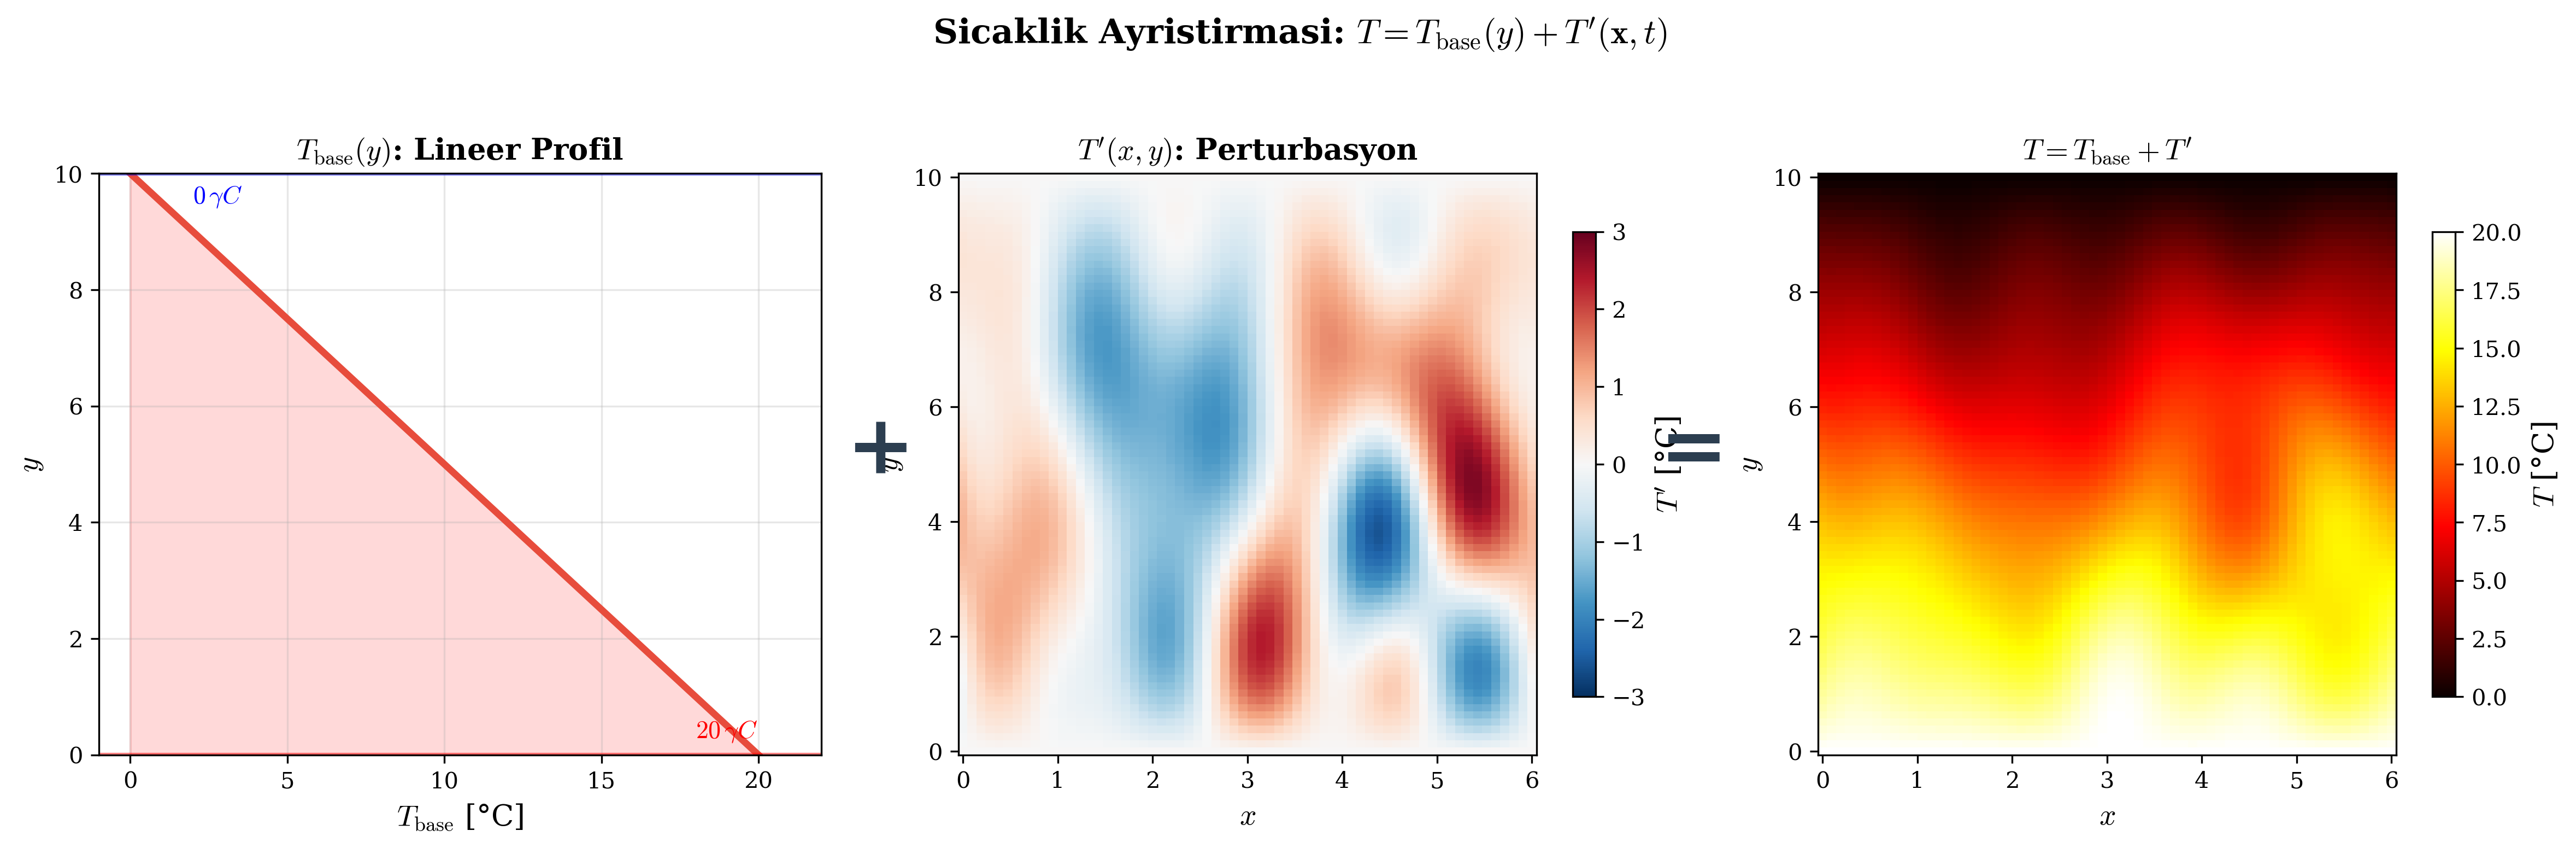
\includegraphics[width=0.90\textwidth]{temperature_decomposition.png}
%    \caption{Sıcaklık ayrıştırması. Sol: $T_{\text{base}}(y)$ lineer profil. Orta: $T'$ pertürbasyon (periyodik, FFT uyumlu). Sağ: $T_{\text{total}} = T_{\text{base}} + T'$.}
%    \label{fig:temperature_decomposition}
%\end{figure}


% ============================================================
\section{Boyutsuz Denklem Sistemi}
\label{sec:bizim_denklemler}

Proje, Boussinesq yaklaşımı altında çalışır (bkz.~Bölüm~\ref{ch:boussinesq}). Boyutsuz değişkenler ile denklem sistemi:

\subsection{Momentum Denklemi}
\begin{equation}
    \boxed{
        \pd{\vect{u}}{t} + (\vect{u} \cdot \gradient)\vect{u}
        = -\gradient p
        + \frac{1}{\Rey} \laplacian \vect{u}
        + \Rich \, T' \, \hat{\vect{e}}_y
        + \vect{F}
    }
    \label{eq:momentum_bizim}
\end{equation}

Terimlerin fiziksel anlamları:
\begin{itemize}
    \item $(\vect{u} \cdot \gradient)\vect{u}$: Adveksiyon --- akışkanın kendini taşıması (nonlineer terim).
    \item $-\gradient p$: Basınç gradyanı --- kütlenin korunumunu zorlar ($\divergence \vect{u} = 0$).
    \item $\frac{1}{\Rey} \laplacian \vect{u}$: Visköz difüzyon --- kinetik enerjiyi ısıya çevirir.
    \item $\Rich \, T' \, \hat{\vect{e}}_y$: Kaldırma kuvveti --- sıcaklık pertürbasyonundan kaynaklanan dikey kuvvet.
    \item $\vect{F}$: Dış zorlama (Kolmogorov forcing, (\ref{eq:kolmogorov_forcing})).
\end{itemize}

\subsection{Sıcaklık Pertürbasyon Denklemi}
\begin{equation}
    \boxed{
        \pd{T'}{t} + (\vect{u} \cdot \gradient)T'
        = \frac{1}{\Rey \, \Pran} \laplacian T'
        + v \, \frac{\Delta T}{L_y}
    }
    \label{eq:temperature_bizim}
\end{equation}
Son terim, Bölüm~\ref{sec:sicaklik_ayristirma}'daki türetimden gelen kaynak terimidir.

\subsection{Süreklilik Denklemi}
\begin{equation}
    \boxed{\divergence \vect{u} = 0}
    \label{eq:continuity_bizim}
\end{equation}
Boussinesq yaklaşımında hız alanı solenoidaldir. Bu koşul, her zaman adımında Projection nöronu tarafından sağlanır.

\subsection{Bileşen Formu}

Açık bileşen yazımı (hesaplama implementasyonu için):
\begin{align}
    \pd{u}{t} + u\pd{u}{x} + v\pd{u}{y} + w\pd{u}{z}
    &= -\pd{p}{x} + \frac{1}{\Rey}\left(\pdd{u}{x} + \pdd{u}{y} + \pdd{u}{z}\right) + F_x
    \label{eq:u_component} \\[6pt]
    \pd{v}{t} + u\pd{v}{x} + v\pd{v}{y} + w\pd{v}{z}
    &= -\pd{p}{y} + \frac{1}{\Rey}\left(\pdd{v}{x} + \pdd{v}{y} + \pdd{v}{z}\right) + \Rich \, T'
    \label{eq:v_component} \\[6pt]
    \pd{w}{t} + u\pd{w}{x} + v\pd{w}{y} + w\pd{w}{z}
    &= -\pd{p}{z} + \frac{1}{\Rey}\left(\pdd{w}{x} + \pdd{w}{y} + \pdd{w}{z}\right)
    \label{eq:w_component} \\[6pt]
    \pd{T'}{t} + u\pd{T'}{x} + v\pd{T'}{y} + w\pd{T'}{z}
    &= \frac{1}{\Rey \, \Pran}\left(\pdd{T'}{x} + \pdd{T'}{y} + \pdd{T'}{z}\right) + \frac{v \, \Delta T}{L_y}
    \label{eq:Tprime_component}
\end{align}
Önemli: Kaldırma kuvveti terimi \textit{yalnızca} $v$-denkleminde (dikey momentum) görülür; $u$ ve $w$ denklemlerinde yer almaz. Benzer şekilde, Kolmogorov forcing ($F_x$) yalnızca $u$-denklemindedir.


% ============================================================
\section{Boyutsuz Sayılar ve Parametre Uzayı}
\label{sec:parametre_uzayi}

\subsection{Boyutsuz Sayıların Tanımı}

\begin{table}[H]
\centering
\caption{Projede kullanılan boyutsuz sayılar.}
\label{tab:boyutsuz_sayilar}
\begin{tabular}{@{}llll@{}}
\toprule
\textbf{Sayı} & \textbf{Tanım} & \textbf{Değer Aralığı} & \textbf{Fiziksel Anlam} \\
\midrule
$\Rey$ & $UL/\nu$ & $5\,000$--$10\,000$ & Atalet / viskozite oranı \\
$\Ray$ & $g\beta\Delta T L^3 / (\nu\kappa)$ & $10^5$--$10^7$ & Kaldırma / difuzyon oranı \\
$\Pran$ & $\nu / \kappa$ & $0.71$ & Momentum / ısı difuzyon oranı (hava) \\
$\Rich$ & $\Ray / (\Rey^2 \Pran)$ & (hesaplanır) & Kaldırma / atalet oranı \\
$\Nus$ & $1 + \langle v T' \rangle \big/ \left(\kappa \frac{\Delta T}{L_y}\right)$ & $\geq 1$ & Toplam / difuzif ısı oranı \\
\bottomrule
\end{tabular}
\end{table}

Richardson sayısı akış rejimini belirleyen anahtar parametredir:
\begin{equation}
    \Rich = \frac{\Ray}{\Rey^2 \, \Pran}
    \label{eq:Ri_definition}
\end{equation}

\subsection{Richardson Sayısı Tablosu}

\begin{table}[H]
\centering
\caption{$\Rich$ değerleri, $\Rey$ ve $\Ray$ kombinasyonları için ($\Pran = 0.71$).}
\label{tab:Ri_values}
\begin{tabular}{@{}l|ccc@{}}
\toprule
$\Rey \backslash \Ray$ & $10^5$ & $10^6$ & $10^7$ \\
\midrule
$5\,000$   & $0.0056$   & $0.056$   & $0.56$     \\
$7\,000$   & $0.0029$   & $0.029$   & $0.29$     \\
$10\,000$  & $0.0014$   & $0.014$   & $0.14$     \\
\bottomrule
\end{tabular}
\end{table}

\subsection{Rejim Analizi}

\begin{itemize}
    \item $\Rich \ll 1$: \textbf{Rüzgâr baskın} (forced convection rejimi). Kolmogorov forcing, kaldırma kuvvetinden çok daha güçlü; sıcaklık pasif skaler gibi taşınır. Bu projede $\Rey = 10\,000$, $\Ray = 10^5$ ile $\Rich \approx 0.0014$: neredeyse tamamen zorlanmış konveksiyon.

    \item $\Rich \sim \mathcal{O}(0.1\text{--}1)$: \textbf{Mixed convection} (karışık rejim). Rüzgâr ve kaldırma kuvveti karşılaştırılabilir büyüklükte; en karmaşık fizik. Tilted plume'lar, eğik konveksiyon hücreleri görülür. Bu projede $\Rey = 5\,000$, $\Ray = 10^7$ ile $\Rich \approx 0.56$: mixed convection rejimi.

    \item $\Rich \gg 1$: \textbf{Kaldırma baskın} (natural convection rejimi). Sıcaklık farkı akışı domine eder; rüzgâr küçük bir pertürbasyondur. \textit{Bu projede seçilen parametre aralığında $\Rich > 1$ elde edilemiyor; en yüksek değer $\Rich \approx 0.56$.}
\end{itemize}

Tablodaki değerlere bakarsak, seçilen parametre uzayının $\Rich \sim 0.001$'den $\Rich \sim 0.56$'ya kadar uzandığını görürüz. Bu, zorlanmış konveksiyondan mixed konveksiyona geçişi kapsayan bir aralıktır. Kaldırma baskın rejim ($\Rich \gg 1$) için daha yüksek $\Ray$ veya daha düşük $\Rey$ değerleri gerekir.


% ============================================================
\section{CFL Koşulu ve Zaman Adımı}
\label{sec:cfl}

\subsection{CFL Koşulu}

Courant--Friedrichs--Lewy (CFL) koşulu, açık zaman integrasyon yöntemlerinin kararlılığı için gereklidir:
\begin{equation}
    \mathrm{CFL} = |\vect{u}|_{\max} \cdot \frac{\Delta t}{\Delta x_{\min}} < 1
    \label{eq:cfl}
\end{equation}
Üç boyutlu durumda:
\begin{equation}
    \mathrm{CFL} = \Delta t \left(\frac{|u|_{\max}}{\Delta x} + \frac{|v|_{\max}}{\Delta y} + \frac{|w|_{\max}}{\Delta z}\right) < 1.
    \label{eq:cfl_3d}
\end{equation}

Fiziksel anlam: bir zaman adımında bilgi, en fazla bir grid hücresi kadar ilerleyebilir. Bu koşul ihlal edilirse, sayısal şema dengesiz dalga modlarını üretir ve çözüm patlar.

\subsection{Grid Boyutları}

INNATE grid: $N_x \times N_y \times N_z = 96 \times 160 \times 64$.
\begin{equation}
    \Delta x = \frac{L_x}{N_x} = \frac{6}{96} = 0.0625, \quad
    \Delta y = \frac{L_y}{N_y} = \frac{10}{160} = 0.0625, \quad
    \Delta z = \frac{L_z}{N_z} = \frac{4}{64} = 0.0625.
    \label{eq:grid_spacing}
\end{equation}
Her üç yönde eşit grid aralığı ($\Delta x = \Delta y = \Delta z = 0.0625$) elde edilir. Bu izotropik grid, spektral yöntemler için idealdir.

DNS grid: $N_x \times N_y \times N_z = 192 \times 320 \times 128$. Grid aralığı: $\Delta x_{\text{DNS}} = 0.03125$.

\subsection{Zaman Adımı Analizi}

Seçilen zaman adımı: $\Delta t = 0.005$.

\textbf{Konvektif CFL:} Tipik türbülant hız $|\vect{u}|_{\max} \sim 3$ varsayımı ile:
\begin{equation}
    \mathrm{CFL}_{\text{conv}} = 3 \times \frac{0.005}{0.0625} = 0.24 \quad (\text{güvenli}).
    \label{eq:cfl_check}
\end{equation}

\textbf{Difüzif CFL:} 3B'de altı komşu nokta olduğundan:
\begin{equation}
    \Delta t < \frac{\Delta x^2}{6\nu} = \frac{0.0625^2}{6 / \Rey}
    \label{eq:diffusive_cfl}
\end{equation}
$\Rey = 5000$ ($\nu = 2 \times 10^{-4}$) için:
\[
    \Delta t < \frac{3.906 \times 10^{-3}}{1.2 \times 10^{-3}} \approx 3.26.
\]
Difüzif kararlılık sınırı çok rahat sağlanır ($\Delta t = 0.005 \ll 3.26$). Bu beklenendir: yüksek $\Rey$'de konvektif CFL kısıtlayıcıdır, difüzif değil.


% ============================================================
\section{Başlangıç Koşulları}
\label{sec:baslangic}

Simülasyon aşağıdaki başlangıç koşulları ile başlatılır:

\subsection{Hız Alanı}
\begin{equation}
    u(x, y, z, 0) = \epsilon_u \cdot \eta_u(x, y, z), \quad
    v(x, y, z, 0) = \epsilon_v \cdot \eta_v(x, y, z), \quad
    w(x, y, z, 0) = \epsilon_w \cdot \eta_w(x, y, z)
    \label{eq:ic_velocity}
\end{equation}
Burada $\eta_u, \eta_v, \eta_w \sim \mathcal{N}(0, 1)$ standart normal dağılımlı rastgele alanlar ve $\epsilon \sim 0.01$ küçük bir genlik faktörüdür.

\textbf{Neden küçük pertürbasyon?} Sıfır hız alanı ($\vect{u} = \vect{0}$) bir denge durumudur, ancak \textit{kararsız} bir dengedir (yüksek $\Rey$ ve $\Ray$ için). Küçük pertürbasyon, doğal instabiliteleri tetikler ve simülasyonun gerçekçi türbülant duruma geçmesini sağlar.

\begin{remark}
Başlangıç pertürbasyonu sonrası Projection uygulanarak $\divergence \vect{u} = 0$ sağlanır. Rastgele alan dolaylı olarak divergence-free değildir; Projection bu hatayı düzeltir.
\end{remark}

\subsection{Sıcaklık Alanı}
\begin{equation}
    T'(x, y, z, 0) = \epsilon_T \cdot \eta_T(x, y, z), \quad \epsilon_T \sim 0.01
    \label{eq:ic_temperature}
\end{equation}
Toplam sıcaklık: $T(x, y, z, 0) = T_{\text{base}}(y) + T'(x, y, z, 0)$.

\subsection{Basınç Alanı}
\begin{equation}
    p(x, y, z, 0) = 0.
    \label{eq:ic_pressure}
\end{equation}
Basınçın sıfırdan başlaması sorun oluşturmaz: Projection nöronu her adımda basıncı $\divergence \vect{u} = 0$'ı sağlayacak şekilde yeniden hesaplar. Başlangıç değeri ilk adımda düzeltilir.

\subsection{Spin-Up Dönemi}

Başlangıç koşullarından istatistiksel kararlı duruma ulaşmak için bir ``spin-up'' dönemi gereklidir. Bu dönemde:
\begin{enumerate}
    \item Kolmogorov forcing, ortalama akışı kurar.
    \item Sıcaklık farkı, konvektif hücreleri geliştirir.
    \item Enerji kaskadı oluşur: büyük ölçeklerden küçük ölçeklere enerji akar.
    \item \"{I}statistiksel denge kurulur: enerji üretimi $\approx$ dissipasyon.
\end{enumerate}
Spin-up süresi probleme bağlıdır; tipik olarak $t_{\text{spin-up}} \sim 10$--$50$ büyük ölçek zaman birimi ($L_y / U$).


% ============================================================
\section{Bölüm Özeti}
\label{sec:problem_ozet}

Bu bölümde tanımlanan problem:

\begin{itemize}
    \item $6 \times 10 \times 4$ boyutlu, üç yönde periyodik kutu.
    \item Alt sıcak ($20\,^{\circ}\mathrm{C}$), üst soğuk ($0\,^{\circ}\mathrm{C}$) $\to$ kaldırma kuvveti.
    \item Kolmogorov forcing $\to$ yatay rüzgâr etkisi.
    \item Sıcaklık ayrıştırması: $T = T_{\text{base}} + T'$ ile periyodik BC uyumu.
    \item 4 alan değişkeni: $u, v, w, T'$ (basınç Projection ile hesaplanır).
    \item 3 kontrol parametresi: $\Rey \in [5000, 10000]$, $\Ray \in [10^5, 10^7]$, $\Pran = 0.71$.
    \item Grid: $96 \times 160 \times 64$ (INNATE), $192 \times 320 \times 128$ (DNS).
    \item $\Delta t = 0.005$, $\mathrm{CFL} \approx 0.24$.
\end{itemize}

Sonraki bölümde (Bölüm~\ref{ch:innate_mimari}), bu denklemlerin her teriminin nasıl bir INNATE nöronuna dönüştüğünü ve ağ yapısını göreceğiz.

% ============================================================
% Bölüm 9: INNATE Mimarisi
% ============================================================

\chapter{INNATE Mimarisi}
\label{ch:innate_mimari}

INNATE (Interpretable Neural Network Architecture for Turbulence Emulation), klasik neural operator'lardan temel bir farkla ayrılır: ağdaki her nöron bir \textit{fiziksel operatör}dür. MLP katmanları, attention mekanizmaları veya kara kutu bileşenler yoktur. \"Oğrenilebilir parametreler doğrudan fiziksel anlamlara sahiptir: etkin viskozite, adveksiyon modulatörü, kaldırma kuvveti katsayısı gibi.


% ============================================================
\section{Temel Prensip: Fizik = Ağ Yapısı}
\label{sec:temel_prensip}

Geleneksel neural network'lerde:
\[
    h = \sigma(Wx + b)
\]
nöronu, öğrenilen ağırlık matrisi $W$ ve bias $b$ ile girdiye lineer dönüşüm + aktivasyon uygular. Bu nöron \textit{evrensel} ama \textit{yorumlanamazdır}: $W$'nun fiziksel anlamı yoktur.

INNATE'te her nöron, NS denklemlerinin belirli bir terimini hesaplar:
\begin{align}
    \text{Advection nöronu:} &\quad -\alpha \cdot (\vect{u} \cdot \gradient)\vect{u} \\
    \text{Diffusion nöronu:} &\quad \nu_{\text{eff}} \cdot \laplacian \vect{u} \\
    \text{Projection nöronu:} &\quad \vect{u} - \gradient \phi \quad (\divergence \vect{u} = 0) \\
    \text{Buoyancy nöronu:} &\quad \beta_{\text{eff}} \cdot \Rich \cdot T' \cdot \hat{\vect{e}}_y
\end{align}
Her nöronün bir veya birkaç öğrenilebilir parametresi vardır ($\alpha$, $\nu_{\text{eff}}$, $\beta_{\text{eff}}$, \ldots). Eğitim sonunda bu parametreler fiziksel olarak yorumlanabilir: ``model hangi etkin viskoziteyi öğrendi?'' sorusu doğrudan cevaplanabilir.

\begin{remark}
Parametre sayısı perspektifi: INNATE yaklaşık $\sim 10$K parametreye sahipken, tipik bir FNO modeli $\sim 10^6$ parametreye sahiptir. Bu $100\times$ fark, INNATE'in yorumlanabilirliğinin ve fiziksel çerçevesinin doğrudan sonucudur.
\end{remark}


% ============================================================
\section{Nöron Tipleri}
\label{sec:noron_tipleri}

Aşağıda her nöron tipi, matematiksel formu, fiziksel anlamı ve öğrenilebilir parametreleri ile birlikte tanımlanmıştır.


% --- 1. Advection3D ---
\subsection{Advection3D: Nonlineer Konveksiyon}
\label{sec:advection_noron}

\textbf{Fiziksel anlam:} Akışkanın momentumunu kendi hız alanıyla taşıması.

\textbf{Matematiksel form (convective form):}
\begin{equation}
    \mathcal{A}(\vect{u}) = -\alpha_{\text{adv}} \cdot (\vect{u} \cdot \gradient)\vect{u}
    \label{eq:advection_neuron}
\end{equation}
Bileşen yazımı:
\begin{equation}
    \mathcal{A}_i = -\alpha_{\text{adv}} \cdot \sum_{j=1}^{3} u_j \pd{u_i}{x_j}, \quad i \in \{1, 2, 3\}
    \label{eq:advection_component}
\end{equation}

\textbf{Hesaplama adımları:}
\begin{enumerate}
    \item Türevler spektral olarak hesaplanır: $\widehat{\partial u_i / \partial x_j} = i k_j \hat{u}_i$.
    \item Fiziksel uzaya döndürülür: $\partial u_i / \partial x_j = \text{IFFT}(\ldots)$.
    \item Çarpım fiziksel uzayda yapılır: $u_j \cdot (\partial u_i / \partial x_j)$.
    \item \textbf{Dealiasing} uygulanır (2/3 kuralı veya mode-index bazlı).
\end{enumerate}

\textbf{Dealiasing neden gerekli?} Fiziksel uzayda iki alanın çarpımı, Fourier uzayında konvolüsyona karşılık gelir. Eğer her iki alan $k_{\max}$'a kadar modlara sahipse, çarpım $2k_{\max}$'a kadar modlar üretir. Grid sadece $k_{\max}$'a kadar çözebildiğinden, $k_{\max}$'ı aşan modlar düşük modlara ``katlanır'' (aliasing). 2/3 kuralı, $k > (2/3)k_{\max}$ modlarını sıfırlayarak bu hatanın birikmesini önler.

\textbf{Öğrenilebilir parametre:}
\begin{itemize}
    \item \texttt{advection\_modulator} $(\alpha_{\text{adv}})$: başlangıç değeri $= 1.0$, klamplama: $[0.5, 2.0]$.
\end{itemize}
$\alpha_{\text{adv}} = 1$ tam adveksiyon demektir. Model bunu biraz büyütebilir veya küçültebilir: LES gridinde çözülemeyen ince yapıların adveksiyon üzerindeki etkisini modelle.


% --- 2. Diffusion ---
\subsection{Diffusion: Visköz Yayılma}
\label{sec:diffusion_noron}

\textbf{Fiziksel anlam:} Moleküler viskozite tarafından momentumun yayılması.

\textbf{Matematiksel form:}
\begin{equation}
    \mathcal{D}(\vect{u}) = \frac{\nu_{\text{scale}}}{\Rey} \laplacian \vect{u}
    \label{eq:diffusion_neuron}
\end{equation}

\textbf{Hesaplama:} Tamamen spektral uzayda:
\begin{equation}
    \widehat{\laplacian u_i} = -(k_x^2 + k_y^2 + k_z^2) \hat{u}_i = -|\vect{k}|^2 \hat{u}_i
    \label{eq:spectral_laplacian}
\end{equation}
Bu işlem FFT + çarpım + IFFT olarak çok ucuzdur.

\textbf{Öğrenilebilir parametre:}
\begin{itemize}
    \item \texttt{diffusion\_scale} $(\nu_{\text{scale}})$: başlangıç $= 1.0$, klamplama: $[0.1, 3.0]$.
\end{itemize}
$\nu_{\text{scale}} = 1$ dolaylı moleküler viskoziteyi verir. Model bunu $> 1$ yaparak etkin viskoziteyi artırabilir --- LES grid'inde çözülemeyen küçük ölçeklerin dissipasyonunu kaba bir şekilde modellemek için.


% --- 3. EddyViscosity3D ---
\subsection{EddyViscosity3D: LES Nöronu}
\label{sec:eddy_noron}

\textbf{Fiziksel anlam:} Çözülemeyen küçük ölçeklerin büyük ölçekler üzerindeki etkisini modeller (subgrid-scale modeli).

\textbf{Matematiksel form (Smagorinsky):}
\begin{equation}
    \mathcal{E}(\vect{u}) = \divergence \left( \nu_t \, \gradient \vect{u} \right)
    \label{eq:eddy_neuron}
\end{equation}
\begin{equation}
    \nu_t = (C_s \, \bar{\Delta})^2 \, |\tensor{S}|
    \label{eq:smagorinsky}
\end{equation}
\begin{itemize}
    \item $C_s$: Smagorinsky sabiti (öğrenilebilir)
    \item $\bar{\Delta} = (\Delta x \cdot \Delta y \cdot \Delta z)^{1/3}$: filtre genişliği (grid boyutlarından hesaplanır)
    \item $|\tensor{S}| = \sqrt{2 S_{ij} S_{ij}}$: strain rate büyüklüğü
    \item $S_{ij} = \frac{1}{2}\left(\pd{u_i}{x_j} + \pd{u_j}{x_i}\right)$: strain rate tensörü
\end{itemize}

\textbf{Neden kritik?} $96 \times 160 \times 64$ gridi, $\Rey = 10\,000$'de tüm ölçekleri çözecek incelikte değildir. Grid analizi LES skorunu $74/100$ olarak belirlemiştir: makul ama DNS değil. EddyViscosity kapalıyken, çözülemeyen modlara enerji birikir ve 63 saatlik eğitimde görüldüğü gibi patlama (NaN) meydana gelir.

\textbf{Öğrenilebilir parametre:}
\begin{itemize}
    \item \texttt{cs\_value} $(C_s)$: başlangıç $= 0.15$, klamplama: $[0.05, 0.30]$.
\end{itemize}
Klasik Smagorinsky'de $C_s \approx 0.17$ (izotropik türbülans için). INNATE'in bunu öğrenmesine izin verilir: mixed convection'da kanal akışı ve plume yapıları birlikte bulunduğundan, optimal $C_s$ homojen türbülanstan sapabilir.


% --- 4. Projection3D ---
\subsection{Projection3D: Süreklilik Zorlaması}
\label{sec:projection_noron}

\textbf{Fiziksel anlam:} Sıkıştırılamaz akışta $\divergence \vect{u} = 0$ koşulunu zorlar.

\textbf{Matematiksel form (Helmholtz ayrıştırması):}

Herhangi bir hız alanı $\vect{u}^*$ (henüz divergence-free olmayan), şöyle ayrıştırılır:
\begin{equation}
    \vect{u}^* = \vect{u} + \gradient \phi
    \label{eq:helmholtz}
\end{equation}
Burada $\vect{u}$ solenodial ($\divergence \vect{u} = 0$) ve $\gradient \phi$ irrotasyonel kısımdır. Sürekliliği zorlamak için:
\begin{enumerate}
    \item Poisson denklemi çözülür:
    \begin{equation}
        \laplacian \phi = \divergence \vect{u}^*
        \label{eq:poisson}
    \end{equation}
    \item Hız düzeltilir:
    \begin{equation}
        \vect{u} = \vect{u}^* - s_p \cdot \gradient \phi
        \label{eq:projection_correction}
    \end{equation}
\end{enumerate}

\textbf{Spektral çözüm:} Periyodik domain'de Poisson denklemi Fourier uzayında tek bir bölme işlemine dönüşür:
\begin{equation}
    \hat{\phi}(\vect{k}) = \frac{\widehat{\divergence \vect{u}^*}(\vect{k})}{-|\vect{k}|^2}, \quad |\vect{k}| \neq 0; \qquad \hat{\phi}(\vect{0}) = 0
    \label{eq:poisson_spectral}
\end{equation}
Sıfır modu ($\vect{k} = \vect{0}$) ortalama basınca karşılık gelir ve periyodik domain'de belirsizdir; sıfıra sabitlenir.

\textbf{Öğrenilebilir parametre:}
\begin{itemize}
    \item \texttt{pressure\_scale} $(s_p)$: başlangıç $= 1.0$, klamplama: $[0.8, 1.2]$.
\end{itemize}
$s_p = 1$ tam Projection demektir. Model bunu hafifçe ayarlayarak, unrolled time-stepping'de basınç düzeltmesinin ``şiddetini'' optimize edebilir.


% --- 5. Forcing3D ---
\subsection{Forcing3D: Dış Kuvvet}
\label{sec:forcing_noron}

\textbf{Fiziksel anlam:} Kolmogorov body forcing ile rüzgâr etkisi.

\textbf{Matematiksel form:}
\begin{equation}
    \mathcal{F}(y) = A \sin\!\left(\frac{k_f \cdot 2\pi y}{L_y}\right) \hat{\vect{e}}_x
    \label{eq:forcing_neuron}
\end{equation}

\textbf{Öğrenilebilir parametre:}
\begin{itemize}
    \item \texttt{amplitude} $(A)$: başlangıç $= 1.0$, klamplama: $[0.01, 10.0]$.
\end{itemize}
$A$'nın büyüklüğü, enerji enjeksiyon oranını ($\varepsilon_{\text{in}} = \langle \vect{u} \cdot \vect{F} \rangle$) kontrol eder. Eğitim sırasında model, enerji dengesini sağlayacak $A$'yı öğrenir.


% --- 6. Buoyancy3D ---
\subsection{Buoyancy3D: Kaldırma Kuvveti}
\label{sec:buoyancy_noron}

\textbf{Fiziksel anlam:} Sıcaklık pertürbasyonunun dikey momentuma etkisi.

\textbf{Matematiksel form:}
\begin{equation}
    \mathcal{B}(T') = \beta_{\text{eff}} \cdot \Rich \cdot T' \cdot \hat{\vect{e}}_y
    \label{eq:buoyancy_neuron}
\end{equation}

Yalnızca $v$-denklemine katılır. $T' > 0$ (ortalamadan sıcak) olan bölgelerde yukarı kuvvet, $T' < 0$ olan bölgelerde aşağı kuvvet oluşturur.

\textbf{Öğrenilebilir parametre:}
\begin{itemize}
    \item \texttt{buoyancy\_strength} $(\beta_{\text{eff}})$: başlangıç $= 1.0$, klamplama: $[0.0, 50.0]$.
\end{itemize}


% --- 7. ThermalAdvection3D ---
\subsection{ThermalAdvection3D: Sıcaklık Adveksiyonu}
\label{sec:thermal_adv_noron}

\textbf{Fiziksel anlam:} Hız alanının sıcaklık pertürbasyonunu taşıması.

\textbf{Matematiksel form:}
\begin{equation}
    \mathcal{T}_{\text{adv}}(\vect{u}, T') = -(\vect{u} \cdot \gradient)T' = -\left(u\pd{T'}{x} + v\pd{T'}{y} + w\pd{T'}{z}\right)
    \label{eq:thermal_adv_neuron}
\end{equation}

Hesaplama, Advection3D'nin skaler versiyonudur: türevler spektral, çarpımlar fiziksel uzayda, dealiasing uygulanır.


% --- 8. ThermalDiffusion3D ---
\subsection{ThermalDiffusion3D: Sıcaklık Difüzyonu}
\label{sec:thermal_diff_noron}

\textbf{Fiziksel anlam:} Moleküler iletimle sıcaklığın yayılması.

\textbf{Matematiksel form:}
\begin{equation}
    \mathcal{T}_{\text{diff}}(T') = \frac{\kappa_{\text{scale}}}{\Rey \, \Pran} \laplacian T'
    \label{eq:thermal_diff_neuron}
\end{equation}

\textbf{Öğrenilebilir parametre:}
\begin{itemize}
    \item \texttt{kappa\_scale} $(\kappa_{\text{scale}})$: başlangıç $= 1.0$, klamplama: $[0.1, 5.0]$.
\end{itemize}
$\kappa_{\text{scale}} > 1$ etkin termal difuziviteyi artırır, yani çözülemeyen küçük ölçekli termal yapıların difuzif etkisini modeller.


% ============================================================
\section{Parametre Tablosu}
\label{sec:parametre_tablosu}

\begin{table}[H]
\centering
\caption{INNATE nöron parametreleri özeti.}
\label{tab:neuron_params}
\begin{tabular}{@{}llccc@{}}
\toprule
\textbf{Nöron} & \textbf{Parametre} & \textbf{Init} & \textbf{Min} & \textbf{Max} \\
\midrule
Advection3D        & \texttt{advection\_modulator}  & $1.0$  & $0.5$  & $2.0$ \\
Diffusion          & \texttt{diffusion\_scale}      & $1.0$  & $0.1$  & $3.0$ \\
EddyViscosity3D    & \texttt{cs\_value}             & $0.15$ & $0.05$ & $0.30$ \\
Projection3D       & \texttt{pressure\_scale}       & $1.0$  & $0.8$  & $1.2$ \\
Forcing3D          & \texttt{amplitude}             & $1.0$  & $0.01$ & $10.0$ \\
Buoyancy3D         & \texttt{buoyancy\_strength}    & $1.0$  & $0.0$  & $50.0$ \\
ThermalAdvection3D & (parametresiz)                 & ---    & ---    & --- \\
ThermalDiffusion3D & \texttt{kappa\_scale}          & $1.0$  & $0.1$  & $5.0$ \\
\bottomrule
\end{tabular}
\end{table}

\begin{remark}
Başlangıç değerleri, nöronların \textit{tam fizik} (\textit{yani DNS benzeri}) davranışına karşılık gelecek şekilde seçilmiştir. $\alpha_{\text{adv}} = 1$, $\nu_{\text{scale}} = 1$, $\beta_{\text{eff}} = 1$ demek, denklemlerin hiçbir modifikasyon olmadan çözülmesi anlamına gelir. Eğitim, bu değerleri grid çözünürlüğüne ve LES etkilerine göre ince ayarlar.
\end{remark}


% ============================================================
\section{SpectralOps3DAniso: Spektral Operatörler}
\label{sec:spectral_ops}

Tüm nöronların türev hesapları, ortak bir spektral operatörler sınıfı üzerinden yapılır: \texttt{SpectralOps3DAniso}.

\subsection{Neden Anizotropik?}

Domain boyutları eşit değildir ($6 \times 10 \times 4$). Dolayısıyla her yöndeki dalga sayıları farklıdır:
\begin{equation}
    k_x = \frac{2\pi n_x}{L_x}, \quad
    k_y = \frac{2\pi n_y}{L_y}, \quad
    k_z = \frac{2\pi n_z}{L_z}
    \label{eq:aniso_wavenumbers}
\end{equation}
$n_x \in [0, N_x/2]$, $n_y \in [0, N_y/2]$, $n_z \in [0, N_z/2]$ tamsayı mod indeksleridir. Farklı $L_i$ değerleri, aynı mod indeksinin farklı fiziksel dalga sayılarına karşılık gelmesine neden olur.

\subsection{Temel Operatörler}

\begin{description}
    \item[\texttt{gradient($\hat{f}$)}:] Skaler alanın gradyanı:
    $\widehat{\partial f / \partial x_j} = i k_j \hat{f}$.

    \item[\texttt{laplacian($\hat{f}$)}:] Skaler/vektörel Laplacian:
    $\widehat{\laplacian f} = -(k_x^2 + k_y^2 + k_z^2) \hat{f}$.

    \item[\texttt{curl($\hat{\vect{u}}$)}:] Vortisite:
    $\hat{\omega}_i = i \epsilon_{ijk} k_j \hat{u}_k$ (Levi-Civita sembolü ile).

    \item[\texttt{divergence($\hat{\vect{u}}$)}:] $\widehat{\divergence \vect{u}} = i(k_x \hat{u} + k_y \hat{v} + k_z \hat{w})$.

    \item[\texttt{dealias($\hat{f}$)}:] Yüksek modları sıfırla. Mode-index bazlı: $|n_x| > N_x/3$, $|n_y| > N_y/3$ veya $|n_z| > N_z/3$ olan modlar kaldırılır.

    \item[\texttt{solve\_poisson($\hat{f}$)}:] Poisson denklemi:
    $\hat{\phi} = \hat{f} / (-|\vect{k}|^2)$, $\hat{\phi}(\vect{0}) = 0$.
\end{description}

\subsection{Dealiasing: Mode-Index ve Fiziksel $k$}

\"Onemli bir ayrım: Dealiasing işleminde \textit{mode-index} bazlı filtreleme kullanılır, \textit{fiziksel dalga sayısı büyüklüğü} ($|\vect{k}|$) bazlı değil. Nedeni: anizotropik domain'de aynı fiziksel $k$ değeri, farklı yönlerde farklı mod indekslerine karşılık gelir. Mode-index bazlı kural, FFT'nin ürettiği dizin yapısıyla doğrudan uyumludur.


% ============================================================
\section{Forward Pass Akışı}
\label{sec:forward_pass}

Bir zaman adımının INNATE içindeki akışı:

\begin{figure}[H]
\centering
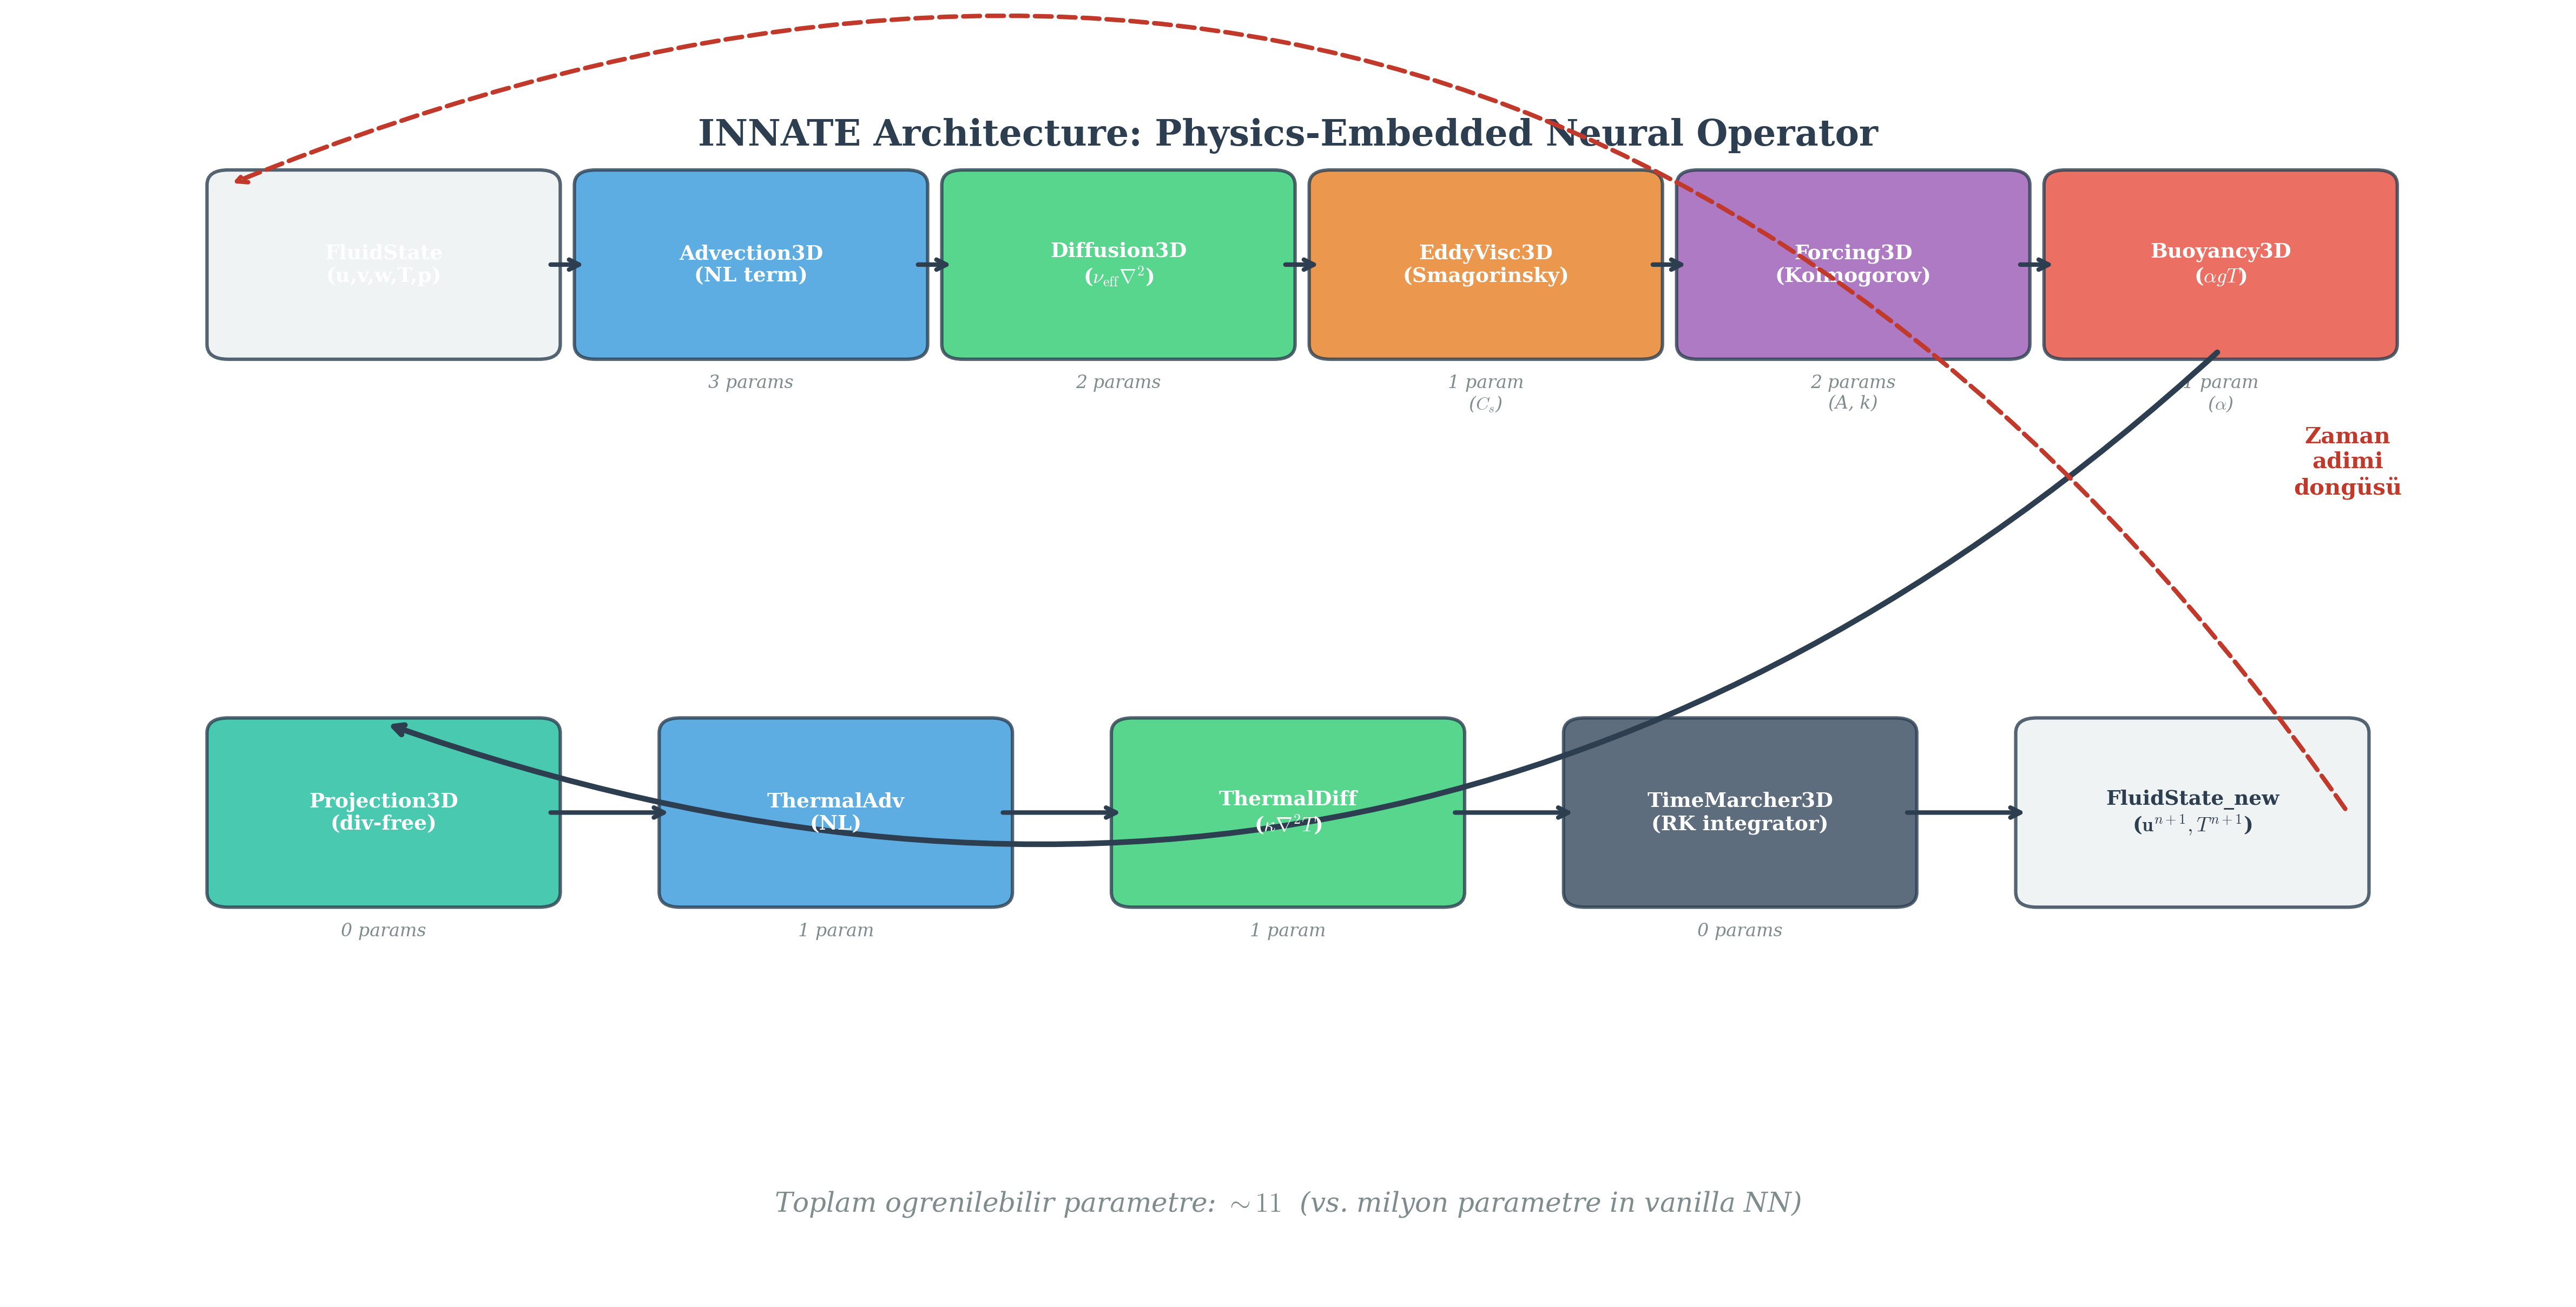
\includegraphics[width=0.9\textwidth]{innate_architecture.png}
\caption{INNATE forward pass akış diyagramı. Her kutu bir fizik nöronunu, yanındaki sayılar öğrenilebilir parametre sayısını gösterir. Akış: momentum $\to$ termal $\to$ projeksiyon $\to$ zaman entegrasyonu.}
\label{fig:innate_architecture}
\end{figure}

\subsection{State Yapısı}

Giriş ve çıkış: \texttt{FluidState3D} --- hız bileşenleri ($u, v, w$), basınç ($p$) ve sıcaklık pertürbasyonu ($T'$).

\subsection{Bir Zaman Adımının Akışı}

\begin{enumerate}
    \item \textbf{Momentum RHS hesabı:}
    \begin{enumerate}
        \item Advection3D: $\vect{R}_{\text{adv}} = -\alpha_{\text{adv}} \cdot (\vect{u} \cdot \gradient)\vect{u}$
        \item Diffusion: $\vect{R}_{\text{diff}} = (\nu_{\text{scale}} / \Rey) \, \laplacian \vect{u}$
        \item EddyViscosity3D: $\vect{R}_{\text{eddy}} = \divergence(\nu_t \gradient \vect{u})$
        \item Forcing3D: $\vect{R}_{\text{force}} = A \sin(k_f \cdot 2\pi y / L_y) \, \hat{\vect{e}}_x$
        \item Buoyancy3D: $\vect{R}_{\text{buoy}} = \beta_{\text{eff}} \cdot \Rich \cdot T' \, \hat{\vect{e}}_y$
    \end{enumerate}
    Toplam: $\vect{R}_u = \vect{R}_{\text{adv}} + \vect{R}_{\text{diff}} + \vect{R}_{\text{eddy}} + \vect{R}_{\text{force}} + \vect{R}_{\text{buoy}}$

    \item \textbf{Sıcaklık RHS hesabı:}
    \begin{enumerate}
        \item ThermalAdvection3D: $R_{T,\text{adv}} = -(\vect{u} \cdot \gradient)T'$
        \item ThermalDiffusion3D: $R_{T,\text{diff}} = (\kappa_{\text{scale}} / \Rey\Pran) \, \laplacian T'$
        \item Kaynak terim: $R_{T,\text{src}} = v \cdot \Delta T / L_y$
    \end{enumerate}
    Toplam: $R_T = R_{T,\text{adv}} + R_{T,\text{diff}} + R_{T,\text{src}}$

    \item \textbf{Zaman entegrasyonu (TimeMarcher3D):}
    RK4 (4. derece Runge--Kutta) şeması:
    \begin{align}
        \vect{k}_1 &= \vect{R}(\vect{q}^n) \\
        \vect{k}_2 &= \vect{R}\!\left(\vect{q}^n + \tfrac{\Delta t}{2} \vect{k}_1\right) \\
        \vect{k}_3 &= \vect{R}\!\left(\vect{q}^n + \tfrac{\Delta t}{2} \vect{k}_2\right) \\
        \vect{k}_4 &= \vect{R}(\vect{q}^n + \Delta t \, \vect{k}_3) \\
        \vect{q}^{n+1} &= \vect{q}^n + \frac{\Delta t}{6}(\vect{k}_1 + 2\vect{k}_2 + 2\vect{k}_3 + \vect{k}_4)
    \end{align}
    Burada $\vect{q} = (u, v, w, T')$ tüm state değişkenlerini temsil eder.

    \item \textbf{Projection (div=0 zorlaması):}
    RK4 sonrasında elde edilen $\vect{u}^*$'a Projection3D uygulanır:
    \[
        \laplacian \phi = \divergence \vect{u}^*, \quad
        \vect{u}^{n+1} = \vect{u}^* - s_p \cdot \gradient \phi
    \]

    \item \textbf{Gauge fix:} $T' \leftarrow T' - \langle T' \rangle$.

    \item \textbf{Çıkış:} \texttt{FluidState3D}$(u^{n+1}, v^{n+1}, w^{n+1}, p^{n+1}, T'^{n+1})$.
\end{enumerate}

\begin{remark}
1 zaman adımı = 1 ağ katmanı. 20 adımlık unrolled eğitim $=$ 20 katmanlı bir ağdan geçiş. Geri yayılım (backpropagation), bu 20 katmandan geriye doğru gradient hesaplar.
\end{remark}


% ============================================================
\section{Yol C: Lokal-Adaptif Parametreler}
\label{sec:yol_c}

Temel INNATE'te her nöron \textit{tek global skaler} parametre kullanır: $\alpha_{\text{adv}}$ her yerde aynıdır. Bu, türbülant akışta yetersiz kalabilir, çünkü lokal koşullar (plume bölgesi vs.\ shear bölgesi) çok farklıdır.

\subsection{Lokal \"{I}nvariantlar}

Her grid noktasında, akış alanından doğrudan hesaplanabilen altı skaler büyüklük:
\begin{equation}
\begin{aligned}
    I_1 &= |\tensor{S}| = \sqrt{2 S_{ij} S_{ij}} && \text{(strain rate büyüklüğü)} \\
    I_2 &= |\vect{\omega}| = \sqrt{\omega_i \omega_i} && \text{(vortisite büyüklüğü)} \\
    I_3 &= Q = \frac{|\vect{\omega}|^2 - |\tensor{S}|^2}{2} && \text{($Q$-kriteri: girdap tanımlama)} \\
    I_4 &= |\gradient T'| && \text{(sıcaklık gradyanı)} \\
    I_5 &= E_{\text{local}} = \tfrac{1}{2}(u^2 + v^2 + w^2) && \text{(lokal kinetik enerji)} \\
    I_6 &= T' && \text{(sıcaklık pertürbasyonu)}
\end{aligned}
\label{eq:invariants}
\end{equation}

Bu büyüklükler, FFT türevlerinden hesaplanır ve otomatik türev (backprop) ile gradient akışını destekler.

\subsection{Adaptif Parametre Formülü}

Global skaler yerine, parametreler her noktada invariantlardan hesaplanır:

\textbf{Lineer versiyon:}
\begin{equation}
    \alpha_{\text{eff}}(\vect{x}) = \alpha_0 + \sum_{m=1}^{6} \alpha_m \, \hat{I}_m(\vect{x})
    \label{eq:linear_modulation}
\end{equation}
7 öğrenilebilir parametre per operatör per katman. $\hat{I}_m$ normalize edilmiş invariantlardır:
\begin{equation}
    \hat{I}_m = \frac{I_m}{\max(I_{m,\text{global}}, \, \varepsilon)}
    \label{eq:invariant_normalization}
\end{equation}
Normalizasyon olmadan invariantlar çok farklı ölçeklerdedir ($|S| \sim \mathcal{O}(100)$, $T' \sim \mathcal{O}(0.01)$) ve eğitim kararsızlaşır.

\textbf{Kuadratik versiyon:}
\begin{equation}
    \alpha_{\text{eff}} = \alpha_0
    + \sum_{m=1}^{6} \alpha_m \hat{I}_m
    + \sum_{m=1}^{3} \alpha_{6+m} \hat{I}_m^2
    + \alpha_{10} \hat{I}_1 \hat{I}_2
    + \alpha_{11} \hat{I}_1 \hat{I}_3
    + \alpha_{12} \hat{I}_2 \hat{I}_3
    \label{eq:quadratic_modulation}
\end{equation}
13 parametre per operatör per katman. Çapraz terimler ($\hat{I}_1 \hat{I}_2$ gibi), strain-vorticity etkileşimini yakalar.

\textbf{Pozitiflik zorlaması (difüziviteler için):}
\begin{equation}
    \nu_{\text{eff}}(\vect{x}) = \text{softplus}\!\left(\nu_0 + \sum_m \nu_m \hat{I}_m + \ldots\right)
    \label{eq:softplus_constraint}
\end{equation}
Softplus: $\text{softplus}(x) = \ln(1 + e^x)$, her zaman $> 0$.

\subsection{Blok Yapısı}

Yol C mimarisinde, 20--25 katman 3--4 bloğa gruplandırılır. Her blokta:
\begin{enumerate}
    \item FFT ile türevler ve invariantlar hesaplanır (blok başında bir kez).
    \item 5--7 katmanda RHS hesabı yapılır (sadece pointwise çarpım ve toplam; FFT yok).
    \item Projection ile $\divergence \vect{u} = 0$ zorlanır.
\end{enumerate}

\subsection{Parametre Bütçesi}

\begin{table}[H]
\centering
\caption{Yol C parametre tahmini (kuadratik versiyon, 4 blok $\times$ 5 katman = 20 katman).}
\label{tab:yol_c_params}
\begin{tabular}{@{}lc@{}}
\toprule
\textbf{Bileşen} & \textbf{Parametre Sayısı} \\
\midrule
5 operatör $\times$ 4 bileşen $(u,v,w,T')$ $\times$ 13 param $\times$ 20 katman & 5,200 \\
EddyViscosity $C_s$ & 1 \\
$\Delta t$ per katman & 20 \\
\midrule
\textbf{Toplam} & $\sim$5,221 \\
\bottomrule
\end{tabular}
\end{table}

Bu $\sim$5K parametre, bir FNO'nun $\sim$10$^6$ parametresinin $\sim$200 katı altındadır; ancak her parametrenin fiziksel anlamı vardır ve lokal adaptasyon yoluyla $983{,}040$ grid noktasında farklı etkin değerler üretir.


% ============================================================
\section{Bölüm Özeti}
\label{sec:mimari_ozet}

\begin{itemize}
    \item INNATE, NS denklemlerinin her terimini bir nöron olarak kodlar.
    \item 8 nöron tipi: Advection3D, Diffusion, EddyViscosity3D, Projection3D, Forcing3D, Buoyancy3D, ThermalAdvection3D, ThermalDiffusion3D.
    \item Her nöronün 0--2 öğrenilebilir parametresi var; hepsi fiziksel anlamlaştırılabilir.
    \item SpectralOps3DAniso, anizotropik domain için türev/Poisson/dealiasing sağlar.
    \item Forward pass: RHS hesabı $\to$ RK4 integrasyon $\to$ Projection $\to$ gauge fix.
    \item Yol C ile parametreler lokal invariantlara bağlanarak uzamsal adaptasyon elde edilir.
    \item Toplam $\sim$5--10K parametre, tamamı yorumlanabilir.
\end{itemize}

Sonraki bölümde (Bölüm~\ref{ch:training}), bu parametrelerin nasıl öğrenildiğini --- loss fonksiyonları, curriculum learning ve eğitim stratejisini --- inceleyeceğiz.

% ============================================================
% Bölüm 10: Training Stratejisi
% ============================================================

\chapter{Training Stratejisi}
\label{ch:training}

INNATE'in $\sim$5--10K parametresi, DNS verisi kullanmadan --- yalnızca fizik tabanlı loss fonksiyonlarıyla eğitilir. Bu yaklaşım, ``physics-only training'' olarak adlandırılır. Bu bölüm, loss fonksiyonlarının fiziksel türetmesini, curriculum learning stratejisini, Re/Ra sweep mekanizmasını ve optimizer seçimlerini kapsar.


% ============================================================
\section{Physics-Only Training Prensibi}
\label{sec:physics_only}

Geleneksel neural operator eğitiminde:
\begin{equation}
    \mathcal{L}_{\text{data}} = \|\vect{u}_{\text{model}} - \vect{u}_{\text{DNS}}\|^2
    \label{eq:data_loss}
\end{equation}
Model çıktısı, yüksek çözünürlüklü DNS referansına yaklaştırılır.

INNATE'te bu yaklaşım kullanılmaz. Nedenleri:
\begin{enumerate}
    \item \textbf{DNS yapılamazlığı:} $\Rey = 10{,}000$'de 3B DNS, $N \sim \Rey^{9/4} \approx 8.4 \times 10^9$ grid noktası gerektirir; bu mevcut donanımla pratik değildir.
    \item \textbf{Yapısal çözücü avantajı:} INNATE'in forward pass'ı zaten NS denklemlerini \textit{yapısal olarak} çözer (Advection, Diffusion, Projection, \ldots). Eğitilen şey denklemlerin kendisi değil, yalnızca birkaç bin fiziksel parametredir.
    \item \textbf{Genelleştirme:} Tek bir $(\Rey, \Ray)$ çiftine göre eğitmek yerine, parametre uzayında sweep yaparak tek bir modelin geniş aralıkta çalışması sağlanır.
\end{enumerate}

\textbf{Eğitim felsefesi:} DNS verisi eğitimde kullanılmaz; yalnızca \textit{validasyon} için saklanır. Model, fiziksel tutarlılık loss'larıyla kalibre edilir.


% ============================================================
\section{Loss Fonksiyonları}
\label{sec:loss_functions}

Yedi loss fonksiyonu, NS denklemlerinin farklı fiziksel kısıtlarını zorlar.


% --- L1: Divergence ---
\subsection{$\mathcal{L}_{\text{divergence}}$: Kütle Korunumu}
\label{sec:loss_divergence}

\begin{equation}
    \boxed{
        \mathcal{L}_{\text{div}} = \left\|\divergence \vect{u}\right\|_2^2
        + 0.1 \, \left\|\divergence \vect{u}\right\|_1
    }
    \label{eq:loss_div}
\end{equation}

\textbf{Türetme:} Sıkıştırılamaz akışta kütle korunumu $\divergence \vect{u} = 0$'ı gerektirir. Projection nöronu bunu her adımda zorlar, ancak RK4 integrasyon sırasında ara aşamalarda küçük sapmalar oluşabilir. Unrolled time-stepping'de bu sapmalar birikebilir.

$L_2$ normu genel sapmayı c\ ezalandırırken, $L_1$ terimi outlier'lara (tek bir noktada büyük divergence) daha hassastır. 0.1 katsayısı, iki terimin göreceli ağırlığını dengeler.


% --- L2: Energy Balance ---
\subsection{$\mathcal{L}_{\text{energy}}$: Kinetik Enerji Dengesi}
\label{sec:loss_energy}

Kinetik enerji bütçe denklemi, NS denklemlerinin hacim ortalamasından çıkar:

\begin{equation}
    \dd{E}{t} = P_{\text{forcing}} + P_{\text{buoyancy}} - \varepsilon
    \label{eq:energy_budget}
\end{equation}
Burada:
\begin{align}
    E &= \frac{1}{2}\langle |\vect{u}|^2 \rangle
    && \text{(hacim-ortalama kinetik enerji)} \label{eq:KE}\\
    Z &= \frac{1}{2}\langle |\vect{\omega}|^2 \rangle
    && \text{(enstrophy)} \label{eq:enstrophy}\\
    \varepsilon &= \frac{2}{\Rey} Z
    && \text{(dissipasyon oranı)} \label{eq:dissipation}\\
    P_{\text{forcing}} &= \langle \vect{u} \cdot \vect{F} \rangle
    && \text{(forcing üretimi)} \label{eq:P_forcing}\\
    P_{\text{buoyancy}} &= \langle v \cdot \Rich \cdot T' \rangle
    && \text{(kaldırma kuvveti üretimi)} \label{eq:P_buoyancy}
\end{align}
$\langle \cdot \rangle$ hacim ortalamasını, $\vect{\omega} = \curl \vect{u}$ vortisiteyi gösterir.

Loss fonksiyonu, bu bütçe denkleminin ihlalini ölçer:
\begin{equation}
    \boxed{
        \mathcal{L}_{\text{energy}} = \left|\dd{E}{t} + \varepsilon - P_{\text{forcing}} - P_{\text{buoyancy}}\right|
    }
    \label{eq:loss_energy}
\end{equation}

$dE/dt$ sonlu farkla yaklaşık olarak hesaplanır: $(E^{n+1} - E^n) / \Delta t$.

\textbf{Fiziksel yorum:} \"{I}statistiksel kararlı durumda $dE/dt \approx 0$ olup enerji üretimi $\approx$ dissipasyon olmalıdır. Geçici durumda ise $dE/dt \neq 0$ olabilir, ancak bütçe denklemi her zaman sağlanmalıdır.


% --- L3: Spectrum ---
\subsection{$\mathcal{L}_{\text{spectrum}}$: Enerji Spektrumu}
\label{sec:loss_spectrum}

Kolmogorov'un 1941 teorisine göre, inertial range'de (enerji enjeksiyon ölçeği ile dissipasyon ölçeği arasında) enerji spektrumu:
\begin{equation}
    E(k) \propto k^{-5/3}
    \label{eq:kolmogorov_spectrum}
\end{equation}

Log-log ölçekte bu $-5/3$ eğimli bir doğru demektir. Loss:
\begin{equation}
    \boxed{
        \mathcal{L}_{\text{spectrum}} = \left(\text{slope}\big(E(k)\big) - \left(-\tfrac{5}{3}\right)\right)^2
    }
    \label{eq:loss_spectrum}
\end{equation}
$\text{slope}(\cdot)$, inertial range'deki $\log E$--$\log k$ doğrusunun eğimidir (lineer regresyon ile).

\textbf{Neden önemli?} Eğer model çok difüzif ise ($\nu_{\text{eff}}$ yüksek), küçük ölçekler yok edilir ve eğim $< -5/3$ (daha dik) olur. Eğer dissipasyon yetersiz ise, eğim $> -5/3$ (daha yatay) olur --- enerji küçük ölçeklere birikir ve patlama riski artar.


% --- L4: Dissipation ---
\subsection{$\mathcal{L}_{\text{dissipation}}$: Dissipasyon Tutarlılığı}
\label{sec:loss_dissipation}

\begin{equation}
    \boxed{
        \mathcal{L}_{\text{diss}} = \left|\varepsilon - \frac{2}{\Rey} Z\right|
    }
    \label{eq:loss_diss}
\end{equation}

\textbf{Türetme:} \"{I}zotropik, homojen türbülansta dissipasyon oranının enstrophy ile ilişkisi:
\begin{equation}
    \varepsilon = 2\nu \langle S_{ij} S_{ij} \rangle = \frac{1}{\Rey}\langle |\vect{\omega}|^2 \rangle = \frac{2}{\Rey} Z
    \label{eq:diss_enstrophy}
\end{equation}
Son eşitlik, homojen türbülans için $\langle S_{ij}S_{ij} \rangle = \frac{1}{2}\langle \omega_i \omega_i \rangle$ bağıntısından gelir (periyodik domain'de geçerli). Bu loss, modelin ürettiği dissipasyon ile vortisiteden hesaplanan dissipasyonun tutarlı olmasını zorlar.


% --- L5: Nusselt ---
\subsection{$\mathcal{L}_{\text{nusselt}}$: Isı Transferi Kısıtı}
\label{sec:loss_nusselt}

Nusselt sayısı, konvektif ısı transferinin difüzif ısı transferine oranıdır:
\begin{equation}
    \Nus = 1 + \frac{\langle v \, T' \rangle}{\kappa \, \Delta T / L_y}
    \label{eq:nusselt_def}
\end{equation}
$\kappa = 1/(\Rey \cdot \Pran)$ boyutsuz termal difüzivitedir. Konveksiyon, ısı transferini \textit{her zaman} artırır (veya aynı bırakır); dolayısıyla:
\begin{equation}
    \Nus \geq 1 \quad \text{(fiziksel zorunluluk)}
    \label{eq:nu_constraint}
\end{equation}

Loss fonksiyonu:
\begin{equation}
    \boxed{
        \mathcal{L}_{\text{nusselt}} = \big[\text{relu}(1 - \Nus)\big]^2
    }
    \label{eq:loss_nusselt}
\end{equation}
$\text{relu}(x) = \max(0, x)$. Eğer $\Nus \geq 1$ ise loss $= 0$ (ihlal yok); $\Nus < 1$ ise c\ eza uygulanır.

\begin{remark}
Bu loss fonksiyonunun önemli bir zayıflığı vardır: $\Nus \geq 1$ sağlandığı anda gradient sıfır olur. Dolayısıyla model, $\Nus = 1.001$ ile tatmin olur ve daha yüksek $\Nus$ değerlerini (ki fiziksel olarak beklenir) öğrenmez. Gelecek versiyonda $\Nus$'u hedef bir aralığa çekecek daha bilgilendirici bir loss kullanmak düşünülebilir.
\end{remark}


% --- L6: Thermal Variance ---
\subsection{$\mathcal{L}_{\text{thermal}}$: Sıcaklık Patlamasi Önleme}
\label{sec:loss_thermal}

\begin{equation}
    \boxed{
        \mathcal{L}_{\text{thermal}} = \big[\text{relu}\big(\text{var}(T') - \text{var}_{\max}\big)\big]^2
    }
    \label{eq:loss_thermal}
\end{equation}

$\text{var}(T') = \langle T'^2 \rangle - \langle T' \rangle^2$ hacim varyansıdır. $\text{var}_{\max}$ probleme bağlı bir üst sınırdır.

\textbf{Neden gerekli?} Sıcaklık pertürbasyonunun kontrolsüz büyümesi, momentum denklemindeki buoyancy terimi ($\Rich \cdot T'$) üzerinden hız alanını da patlatabilir. Bu loss, $T'$'nin varyansını fiziksel sınırlar içinde tutar.


% --- L7: Stability ---
\subsection{$\mathcal{L}_{\text{stability}}$: Enstrophy Patlamasi Önleme}
\label{sec:loss_stability}

\begin{equation}
    \boxed{
        \mathcal{L}_{\text{stability}} = \big[\text{relu}(Z / Z_{\text{ref}} - 10)\big]^2
    }
    \label{eq:loss_stability}
\end{equation}

$Z_{\text{ref}}$, eğitim başlangıcındaki referans enstrophy değeridir. Enstrophy'nin referansın 10 katını aşması fiziksel olmayan bir patlamaya işaret eder.

\begin{remark}
Bu loss da tek yönlüdür: $Z < 10 Z_{\text{ref}}$ olunca gradient yoktur. Ayrıca, eğer eşik çok düşük seçilirse ($Z_{\text{ref}}$ küçükse), bu loss türbülansın gelişmesini \textit{aktif olarak engelleyebilir}. Bu, 63 saatlik başarısız eğitimde görülen sorunlardan biridir.
\end{remark}


% ============================================================
\section{Toplam Loss}
\label{sec:total_loss}

\begin{equation}
    \mathcal{L}_{\text{total}} = \sum_{i=1}^{7} w_i \, \mathcal{L}_i
    \label{eq:total_loss}
\end{equation}

Ağırlıklar $w_i$, curriculum learning'e göre değişir (sonraki bölüm). Tüm loss'lar aynı anda açık olmaz.


% ============================================================
\section{Curriculum Learning}
\label{sec:curriculum}

Tüm loss'ları aynı anda açmak, gradient çatışmasına (gradient conflict) yol açar: farklı loss'lar farklı yönlere gradient üretir ve optimizer hangi yöne gideceğini bilemez. Çözüm: kademeli olarak zorluk artırmak.

\begin{figure}[H]
\centering
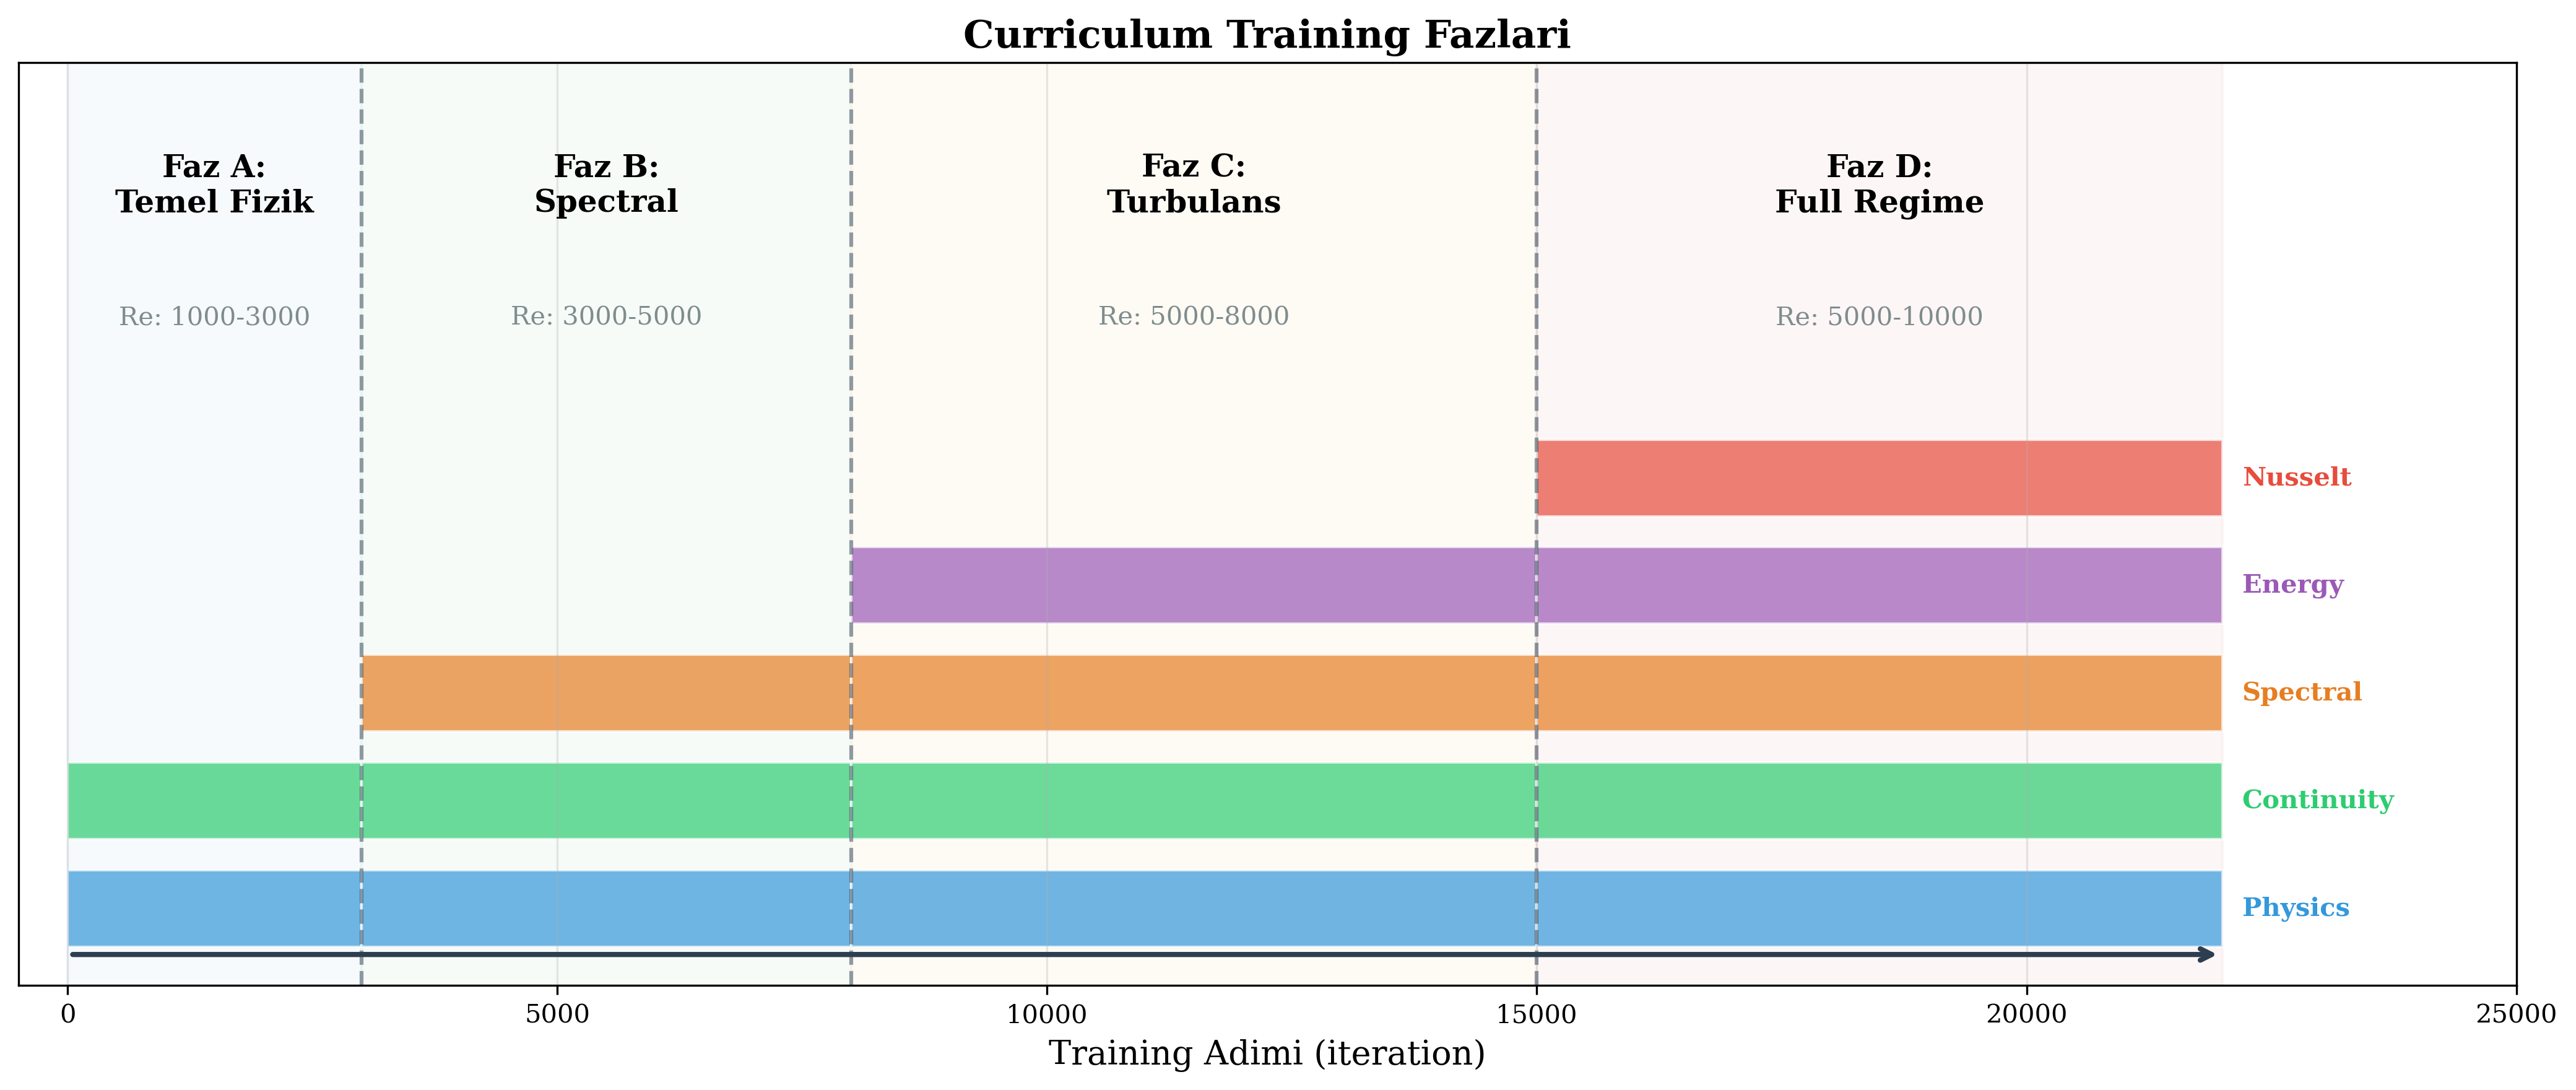
\includegraphics[width=0.9\textwidth]{curriculum_phases.png}
\caption{Curriculum learning fazları. Her faz farklı loss fonksiyonlarını aktifleştirir ve farklı Re/Ra aralıklarında çalışır.}
\label{fig:curriculum_phases}
\end{figure}

\subsection{Faz A: Temel Fizik (Epoch 0--3\,000)}

\begin{itemize}
    \item \textbf{Aktif loss'lar:} $\mathcal{L}_{\text{div}}$, $\mathcal{L}_{\text{thermal}}$
    \item \textbf{Hedef:} Modelin kütle korunumunu öğrenmesi ve sıcaklık alanının patlamaması.
    \item \textbf{$\Rey$, $\Ray$:} Sabit, düşük değerler ($\Rey = 5000$, $\Ray = 10^5$).
\end{itemize}

Bu fazda model, ``temel mekanik'' kurallarını öğrenir: hız alanı divergence-free olmalı, sıcaklık patlamamalı. Enerji spektrumu veya Nusselt sayısına bakılmaz.

\subsection{Faz B: Enerji ve Spektrum (Epoch 3\,000--8\,000)}

\begin{itemize}
    \item \textbf{Aktif loss'lar:} Öncekiler + $\mathcal{L}_{\text{energy}}$, $\mathcal{L}_{\text{spectrum}}$, $\mathcal{L}_{\text{diss}}$, $\mathcal{L}_{\text{nusselt}}$, $\mathcal{L}_{\text{stability}}$
    \item \textbf{Açma yöntemi:} Ramp-up --- ağırlıklar sıfırdan yavaşça yükseltilir:
    \begin{equation}
        w_i(\text{epoch}) = w_{i,\text{max}} \cdot \min\!\left(1, \;\frac{\text{epoch} - 3000}{2000}\right)
        \label{eq:ramp_up}
    \end{equation}
    \item \textbf{Hedef:} Enerji dengesi, Kolmogorov spektrumu, dissipasyon tutarlılığı.
    \item \textbf{$\Rey$, $\Ray$:} Hala düşük veya orta değerler.
\end{itemize}

\subsection{Faz C: Tam Fizik (Epoch 8\,000--15\,000)}

\begin{itemize}
    \item \textbf{Aktif loss'lar:} Tümü tam ağırlıkla.
    \item \textbf{$\Rey$, $\Ray$ sweep:} Her epoch'ta rastgele seçim (bölüm~\ref{sec:re_ra_sweep}).
    \item \textbf{Hedef:} Geniş parametre uzayında genelleştirme.
\end{itemize}

\subsection{Faz D: Non-Boussinesq (Epoch 15\,000--22\,000)}

\begin{itemize}
    \item \textbf{Ek loss'lar:} Kütle korunumu ($d\rho/dt + \divergence(\rho \vect{u}) = 0$), durum denklemi ($p = \rho R T$), global kütle korunumu.
    \item \textbf{Hedef:} Büyük sıcaklık farklarında Boussinesq'in geçerliliğinin ötesine geçmek.
    \item \textbf{Not:} Bu faz, projenin opsiyonel ileri hedefidir.
\end{itemize}

\begin{table}[H]
\centering
\caption{Curriculum fazları özeti.}
\label{tab:curriculum}
\begin{tabular}{@{}llll@{}}
\toprule
\textbf{Faz} & \textbf{Epoch} & \textbf{Loss'lar} & \textbf{$\Rey$ / $\Ray$} \\
\midrule
A & $0$--$3$K & $\mathcal{L}_{\text{div}}$, $\mathcal{L}_{\text{thermal}}$ & Sabit, düşük \\
B & $3$K--$8$K & + enerji, spektrum, diss., nusselt, stab. (ramp) & Düşük--orta \\
C & $8$K--$15$K & Tümü tam ağırlık & Sweep \\
D & $15$K--$22$K & + Non-Boussinesq & Sweep \\
\bottomrule
\end{tabular}
\end{table}


% ============================================================
\section{Re/Ra Sweep}
\label{sec:re_ra_sweep}

Tek bir modelin farklı fiziksel koşullarda çalışması için, eğitim sırasında $\Rey$ ve $\Ray$ sistematik olarak değiştirilir.

\subsection{Mekanizma}

Her epoch'un başında rastgele seçim:
\begin{equation}
    \Rey \in \{5000, 7000, 10000\}, \quad \Ray \in \{10^5, 10^6, 10^7\}
    \label{eq:sweep_values}
\end{equation}
Seçilen değerler modele uygulanır:
\begin{equation}
    \texttt{model.set\_physics}(\Rey, \Ray) \implies
    \begin{cases}
        \nu = 1/\Rey \\
        \kappa = 1/(\Rey \cdot \Pran) \\
        \Rich = \Ray / (\Rey^2 \cdot \Pran)
    \end{cases}
    \label{eq:set_physics}
\end{equation}

\subsection{Neden Randomize?}

Sabit sırayla geçmek (\"once $\Rey = 5000$, sonra $7000$, sonra $10000$) ``catastrophic forgetting''e yol açabilir: model son gördüğü parametreye uzmanlaşır ve öncekini unutur. Rastgele seçim, tüm parametrelerin dengeli biçimde eğitilmesini sağlar.

\subsection{Tek Model, 9 Rejim}

$3 \times 3 = 9$ farklı $(\Rey, \Ray)$ kombinasyonu vardır. Her biri farklı bir akış rejimini temsil eder (Tablo~\ref{tab:Ri_values}). Tek INNATE modeli, tüm bu rejimlerde fiziksel olarak tutarlı sonuçlar üretmelidir. Bu, modelin parametrelerinin $(\Rey, \Ray)$'ya göre ``anlamlı'' adaptasyon yapmasını gerektirir.


% ============================================================
\section{Optimizer ve Hiperparametreler}
\label{sec:optimizer}

\subsection{AdamW}

\begin{equation}
    \theta_{t+1} = \theta_t - \eta \left(\frac{\hat{m}_t}{\sqrt{\hat{v}_t} + \varepsilon} + \lambda \, \theta_t\right)
    \label{eq:adamw}
\end{equation}
\begin{itemize}
    \item $\eta = 3 \times 10^{-4}$: learning rate
    \item $\lambda = 10^{-4}$: weight decay (decoupled, AdamW)
    \item $\beta_1 = 0.9$, $\beta_2 = 0.999$: moment tahmin katsayıları
    \item $\varepsilon = 10^{-8}$: sayısal kararlılık
\end{itemize}

AdamW'nin (decoupled weight decay) tercih nedeni: Adam + $L_2$ regularizasyonda weight decay adaptif öğrenme oranıyla etkileşir ve beklenmeyen davranışlara yol açabilir. AdamW'de weight decay, gradient güncellemesinden bağımsızdır.

\subsection{Learning Rate Şeması}

\textbf{Warmup (0--200 epoch):}
\begin{equation}
    \eta_t = \eta_{\max} \cdot \frac{t}{200}
    \label{eq:warmup}
\end{equation}
Sıfırdan başlayarak lineer olarak artırılır. Neden? Başlangıçta parametreler rastgele civarda olup büyük learning rate gradientleri patlatır.

\textbf{Cosine annealing (200+ epoch):}
\begin{equation}
    \eta_t = \eta_{\min} + \frac{1}{2}(\eta_{\max} - \eta_{\min}) \left(1 + \cos\frac{\pi \, t}{T}\right)
    \label{eq:cosine_annealing}
\end{equation}
Yavaşça düşer, sıfıra yakın bitmez (çok küçük $\eta_{\min}$ ile biter).

\subsection{Gradient Clipping}
\begin{equation}
    \vect{g}_{\text{clip}} = \vect{g} \cdot \min\!\left(1, \; \frac{\text{max\_norm}}{\|\vect{g}\|_2}\right), \quad \text{max\_norm} = 1.0
    \label{eq:grad_clip}
\end{equation}
Gradient normu 1'i aştığında ölçeklenir. Unrolled time-stepping'de (20 adım) gradient'ler patlayabilir; clipping bunu önler.

\subsection{Batch Size ve Unrolling}

\begin{itemize}
    \item \textbf{Batch size:} 1 (tek simülasyon).
    \item \textbf{Unroll length:} 20 zaman adımı.
\end{itemize}

Bir eğitim iterasyonunda model 20 adım ileri çalıştırılır; loss, bu 20 adımın ortalamasıdır. Backpropagation, 20 katmanlık bir ağdan geri geçer. Bu ``unrolled'' yaklaşım, modelin kısa vadeli tahmin yerine çok adımlı evrimde tutarlı olmasını zorlar.

\begin{remark}
Unroll length 20'dir, 1 değil. Tek adımlık eğitimde model, her adımda bağımsız optimize eder ve birikimli hataları öğrenemez. 20 adımlık unrolling, autoregressive error accumulation'ı doğrudan loss'a yansıtır.
\end{remark}


% ============================================================
\section{63 Saatlik Başarısız Eğitimden Dersler}
\label{sec:basarisiz_egitim}

Projenin erken versiyonunda 63 saat süren bir eğitim çalışılmış; sonuçlar başarısız olmuştur. Tespit edilen sorunlar ve çıkarılan dersler:

\begin{enumerate}
    \item \textbf{EddyViscosity3D kapalıydı:} $96 \times 160 \times 64$ grid, $\Rey = 10{,}000$'de DNS çözünürlüğünden çok uzaktır. Subgrid-scale model olmadan, çözülemeyen modlara enerji birikti ve adım 280'de NaN oluştu. \textbf{Ders:} LES nöronu zorunludur.

    \item \textbf{Nusselt loss tek yönlü:} $\text{relu}(1 - \Nus)^2$ formunda $\Nus \geq 1$ olunca gradient sıfırdır. Model, termal coupling'i öğrenemedi; $\Nus = 1.0$ (saf difüzyon) seviyesinde kaldı. \textbf{Ders:} Tek yönlü loss'lar dikkatle kullanılmalı.

    \item \textbf{Stability loss türbülansı engelledi:} $\text{relu}(Z/Z_{\text{ref}} - 10)^2$ formunda, eğer $Z_{\text{ref}}$ küçükse, enstrophy'nin normal türbülant seviyeye ulaşması bile ``patlama'' olarak algılanır ve model türbülansı aktif olarak bastırır. \textbf{Ders:} Referans değerleri dikkatle kalibre edilmeli.

    \item \textbf{Model \%99.7 MLP:} 10,116 / 10,144 parametre MLP'de (PhysicsModulatorMC) olup fizik nöronlarının öğrenilebilir parametreleri cok azınlıktaydı. MLP, 6 global skalerden (E, Z, div, t, T\_mean, Ri) 3 scale faktörü üretmeye çalışıyordu --- yeterli bilgi değil. \textbf{Ders:} MLP kaldırılıp saf INNATE mimarisine geçildi.
\end{enumerate}


% ============================================================
\section{Bölüm Özeti}
\label{sec:training_ozet}

\begin{itemize}
    \item Eğitimde DNS verisi kullanılmaz; 7 fizik tabanlı loss fonksiyonu parametreleri kalibre eder.
    \item Divergence, enerji dengesi, Kolmogorov spektrumu, dissipasyon, Nusselt, termal varyans ve enstrophy kararlılığı zorlanır.
    \item 4 fazlı curriculum: temel fizik $\to$ enerji/spektrum $\to$ tam fizik/sweep $\to$ non-Boussinesq.
    \item Re/Ra sweep ile tek model 9 farklı rejimde eğitilir.
    \item AdamW ($\eta = 3 \times 10^{-4}$), warmup + cosine annealing, gradient clipping.
    \item 20 adımlık unrolled training, batch size 1.
    \item Geçmiş başarısızlıktan çıkarılan dersler: LES zorunlu, tek yönlü loss'lar dikkatli kullanılmalı, MLP yerine saf fizik.
\end{itemize}


% KISIM III — DENEMELER VE BAŞARISIZLIKLAR (yeni içerik 2026-05-09)
% ============================================================
% Bölüm 11: Karşılaşılan Buglar ve Çözümleri
% ============================================================

\chapter{Karşılaşılan Buglar ve Çözümleri}
\label{ch:buglar}

Bu bölüm, INNATE projesinin yaklaşık üç ay süren geliştirme döneminde karşılaşılan sekiz kritik hatayı ve bunların nasıl teşhis edilip çözüldüğünü kronolojik olarak ele alır. Bilimsel yazımda genellikle yalnızca \textit{nihai sonuç} aktarılır; başarısız denemeler, yanlış teşhisler ve geri alınan kararlar gizlenir. Oysa bir lisans tezinin asıl katkısı, yapılan deneylerin niceliğinden çok, bu deneylerden çıkarılan derslerdedir. Bu nedenle bölüm boyunca her bug için aynı şablon kullanılacaktır:

\begin{enumerate}
    \item \textbf{Belirti:} Modelin ürettiği gözlemlenebilir hata (NaN, ıraksak loss, fiziksel olarak yanlış metrik).
    \item \textbf{Tanı:} Hatanın nasıl izole edildiği; hangi loglar, hangi araçlar, hangi ablation çalışmaları kullanıldı.
    \item \textbf{Kök neden:} Fizik, sayısal yöntem veya makine öğrenmesi açısından yapısal açıklama.
    \item \textbf{Çözüm:} Uygulanan kod/parametre/mimari değişiklik.
    \item \textbf{Öğrenilen ders:} Aynı problemin gelecekte tekrarlanmaması için sıkıştırılmış bir kıssadan hisse.
\end{enumerate}

Bu sekiz hatadan üçü makine öğrenmesi karakterinde (loss tasarımı, mimari coupling, optimizer davranışı), ikisi sayısal analiz karakterinde (CFL, von Neumann), biri yazılım altyapısı (\texttt{torch.compile}), biri fizik-tabanlı integrasyon (TBPTT-rollout uyumsuzluğu) ve sonuncusu kapasite-aktivasyon dengesizliği üzerinedir. Hepsi birlikte, ``saf-fizik nöral CFD'' yaklaşımının pratik sınırlarını çizen bir harita oluşturur.


% ============================================================
\section{Amplitude Pumping --- Loss Çatışması ve Metrik Sömürüsü}
\label{sec:bug_amplitude_pumping}

\paragraph{Tarih:} Mart 2026 sonu, \texttt{INNATE v2} eğitimleri.

\subsection*{Belirti}

Modelin ürettiği hız alanı incelendiğinde, hacim-ortalama kinetik enerjinin (\,$\langle |\vect{u}|^2 \rangle / 2$\,) beklenenden \textit{anormal} biçimde yüksek seyrettiği gözlendi. Spektrum eğimi $-5/3$'ten uzak (ortalama $-2.4$ civarı), ancak toplam TKE referans LES'in bazı durumlarda iki katına ulaşıyordu. Yani enerji vardı, fakat doğru ölçeklerde \textit{değildi}: büyük ölçekli yapılar şişmiş, inertial range yok olmuştu. Bu durum literatürde ``amplitude pumping'' (genlik şişirme) olarak bilinen bir tür metrik sömürüsünün (\textit{metric hacking}) klasik tezahürüydü.

\subsection*{Tanı}

İlk eğitim koşusunda yedi loss fonksiyonu (Bölüm \ref{ch:training}) bulunuyordu; ancak iterasyonlar sırasında problem-spesifik düzeltmeler için bu sayı 27'ye çıkmıştı. \texttt{anti\_laminar} ve \texttt{tke\_ref} olarak adlandırılan iki ek loss, modelin laminer bir çözüme yakınsamasını engellemek üzere tasarlanmıştı:

\begin{equation}
    \mathcal{L}_{\text{anti-lam}} = \mathrm{ReLU}\!\left( \mathrm{TKE}_{\min} - \langle |\vect{u}'|^2 \rangle \right)^2,
    \qquad
    \mathcal{L}_{\text{tke-ref}} = \left( \log \mathrm{TKE} - \log \mathrm{TKE}_{\text{LES}} \right)^2.
\end{equation}

Ablation deneyinde bu iki loss tek tek kapatıldığında modelin TKE'si referans LES değerine \textit{aşağıdan} yaklaşıyor, ancak Cs ve $\kappa$ MLP başlığı (\texttt{PhysicsModulator}) negatif Smagorinsky katsayısı üretmeye başlıyordu: $\mathrm{Cs} \approx -0.04$. Eddy viscosity'nin negatif olması, fiziksel olarak \textit{geri-saçılım} (backscatter) anlamına gelir; ancak burada bu fenomen değil, optimizerın loss yüzeyinde keşfettiği bir \textit{kestirme yol} idi. Codex danışmanlığı (2026-04-02) bu davranışı şöyle özetledi: ``Loss \texttt{tke\_ref} eksi yönlü kapanırsa, $\nu_t$'yi negatife çek; $\mathrm{TKE}$ otomatik şişer. Optimizer fiziksel anlam aramaz, gradient takip eder.''

\subsection*{Kök neden}

Sorun, loss fonksiyonlarının çelişik kısıtlar dayatmasıydı. Yedi temel loss (Bölüm \ref{ch:training}) zaten \textit{kapalı} bir bütçe denklemi tanımlıyordu. Ek loss'lar bu kapalı sistemin üzerine yamandığında, optimizer iki gradyan vektörünün dengelendiği patolojik bir minimum buluyordu:

\begin{equation}
    \nabla_\theta \mathcal{L}_{\text{tke-ref}} \;\approx\; -\,\nabla_\theta \mathcal{L}_{\text{spectrum}},
\end{equation}

yani spektrumu düzeltmenin maliyeti TKE'yi düşürmek olduğu için, model her ikisini de optimize edemiyor; hem TKE hem spektrum için \textit{ortalama bir uzlaşma} bulamıyordu. Kapasitesi sınırlı bir modelin (Cs/$\kappa$ MLP'sinin yalnızca 28 trainable parametresi vardı), bu çelişkiyi çözmek yerine en kolay kestirme yolu (negatif viskozite) tercih etmesi beklendik bir davranıştı.

\subsection*{Çözüm}

27 Nisan -- 29 Nisan 2026 arasında üç katmanlı bir mimari müdahale uygulandı:

\begin{itemize}
    \item \textbf{Tier 1 --- Kanonik parametreler dondurma:} INNATE nöronlarındaki 120 fiziksel parametre (\texttt{buoyancy\_strength}, \texttt{advection\_modulator}, \texttt{forcing.amplitude}, $\ldots$) literatürdeki kanonik değerleriyle (1.0) sabitlendi. Bu parametrelerin trainable olması, modelin fiziği değil ``sayıları'' optimize etmesine neden oluyordu.
    \item \textbf{Tier 2 --- PDE residual loss eklendi:} Boussinesq denklemlerinin yerel residual'ı doğrudan loss'a yazıldı:
    \begin{equation}
        \mathcal{L}_{\text{NS-res}} = \left\| \pd{\vect{u}}{t} + (\vect{u}\cdot\gradient)\vect{u} + \gradient p - \frac{1}{\Rey}\laplacian\vect{u} - \Rich\,T'\,\hat{\vect{e}}_z \right\|_2^2,
    \end{equation}
    \begin{equation}
        \mathcal{L}_{\text{th-res}} = \left\| \pd{T'}{t} + (\vect{u}\cdot\gradient)T' - \frac{1}{\Rey \Pran}\laplacian T' \right\|_2^2.
    \end{equation}
    Bu iki residual, loss yüzeyindeki kestirme yolları kapatır: ``negatif $\nu_t$'' artık residual'ı şişirir, dolayısıyla optimizer için cazip olmaktan çıkar.
    \item \textbf{Tier 3 --- Loss minimalizasyonu:} 27 loss, fiziksel olarak \textit{bağımsız} 5 temele indirildi:
    $\mathcal{L}_{\text{NS-res}}$, $\mathcal{L}_{\text{th-res}}$, $\mathcal{L}_{\text{div}}$, $\mathcal{L}_{\text{corr}}$ (uzun-zamanlı korelasyon), $\mathcal{L}_{\text{spec}}$ (yalnızca \textit{eğim}, genlik değil).
\end{itemize}

\textbf{Önemli bir alt-detay:} $\mathcal{L}_{\text{spec}}$ yalnızca spektrumun \textit{şeklini} (eğimini) cezalandıracak biçimde formüle edildi:

\begin{equation}
    \mathcal{L}_{\text{spec-shape}} = \left\| \frac{d}{d\log k}\log E_{\text{model}}(k) - \frac{d}{d\log k}\log E_{\text{LES}}(k) \right\|_2^2 \quad (k \in [k_{\text{IR-min}}, k_{\text{IR-max}}]),
\end{equation}

böylece TKE'nin mutlak değeri spektrum loss'undan etkilenmez; mutlak değer yalnızca residual'lar tarafından belirlenir.

\subsection*{Öğrenilen ders}

\begin{remark}
\textit{Loss çatışması, kapasitesi düşük modellerde her zaman metrik sömürüsüne yol açar. Çok sayıda ağırlıklandırılmış loss, az sayıda fiziksel-bağımsız loss'tan \textbf{daha kötüdür}: gradient yönünü belirsizleştirir ve optimizera kestirme yol arama fırsatı sunar. Eğer iki loss aynı niceliği farklı yollardan ölçüyorsa, biri gereksizdir; aynı niceliği farklı yönlerde itiyorsa, en azından biri yanlıştır.}
\end{remark}


% ============================================================
\section{MLP Çıkış Başlığının Ayrıştırılması --- Reynolds Analojisinin Kırılması}
\label{sec:bug_mlp_split}

\paragraph{Tarih:} 17--18 Nisan 2026.

\subsection*{Belirti}

Modelin termal alt-grid kapanışı (\texttt{kappa\_t}) eğitim sırasında neredeyse sıfıra (\,$\kappa_t / \kappa \approx 10^{-2}$\,) düştü. Sonuç olarak Nusselt sayısı LES referansından çok aşağıda kaldı (Nu $\approx 8$, LES'in $\approx 39$). Momentum SGS (\,$\nu_t$\,) ise makul aralıkta kalmaya devam etti. Bu durum, modelin termal türbülansı ``kapatıp'' yalnızca momentum türbülansını öğrendiği bir asimetri ortaya çıkardı.

\subsection*{Tanı}

\texttt{PhysicsModulator} sınıfının ileri yayılım kodu incelendiğinde, MLP çıkış başlığının (\texttt{fc2}) iki ayrı doğrusal projeksiyon kullandığı görüldü:

\begin{lstlisting}[language=Python,caption={MLP çıkış başlığı: ayrılmış (hatalı) versiyon}]
# Kapsule tani: ayrik baslik
self.fc2_cs    = nn.Linear(hidden, 1, bias=True)   # Cs(x,y,z) icin
self.fc2_kappa = nn.Linear(hidden, 1, bias=True)   # kappa_coeff(x,y,z) icin

# ileri yayilim
h = self.act(self.fc1(features))
log_cs    = self.fc2_cs(h).squeeze(-1)             # bagimsiz cikti
log_kappa = self.fc2_kappa(h).squeeze(-1)          # bagimsiz cikti
\end{lstlisting}

Eğitim boyunca \texttt{fc2\_kappa.weight}'in normu izlendiğinde, modelin bu başlığı \textit{aktif olarak öldürdüğü} ortaya çıktı: ağırlıklar logaritmik olarak küçülerek \texttt{kappa\_coeff} çıktısını taban değer olan $0.01$'e yapıştırıyordu. CFD-expert ajanı bu davranışı ``Reynolds analojisinin kırılması'' olarak etiketledi.

\subsection*{Kök neden}

Klasik LES kapanışında momentum ve termal eddy diffusivity'ler türbülanslı Prandtl sayısı $\Pran_t$ üzerinden \textit{yapısal olarak kuplajlıdır}:

\begin{equation}
    \kappa_t = \frac{\nu_t}{\Pran_t}, \qquad \Pran_t \approx 0.7\text{--}1.0 \text{ (mixed convection)}.
    \label{eq:reynolds_analogy}
\end{equation}

Bu denklem yalnızca pratik bir yaklaşım değil; aynı zamanda momentum ve ısı taşınımının aynı eddy yapıları tarafından yapıldığını söyleyen \textit{Reynolds analojisinin} ifadesidir. MLP başlığını ayırmak, optimizera ``$\nu_t$ ve $\kappa_t$ birbirinden bağımsızdır'' demek anlamına geliyordu. Loss yüzeyinde $\kappa_t \to 0$, $\nu_t > 0$ kombinasyonu, termal residual'ı kısa vadede düşürmenin (yüksek difüzyon olmadığı için $T'$ alanı daha az pürüzlü) bir kestirme yoluydu --- aynı bir önceki bölümdeki metrik sömürüsünün bir varyantı.

\subsection*{Çözüm}

MLP yapısı yeniden birleştirildi ve $\Pran_t$ \textit{öğrenilebilir tek bir log-skaler} olarak tanımlandı:

\begin{lstlisting}[language=Python,caption={Yapısal Reynolds analojisi: birleşik başlık}]
# Reynolds analojisi: tek baslik + log-Pr_t
self.fc2_cs        = nn.Linear(hidden, 1, bias=True)            # Cs(x,y,z)
self.log_inv_Pr_t  = nn.Parameter(torch.zeros(1))               # log(1/Pr_t)

# ileri yayilim
log_cs   = self.fc2_cs(self.act(self.fc1(features))).squeeze(-1)
Cs       = torch.exp(log_cs).clamp(min=1e-3, max=0.3)
nu_t     = (Cs * delta) ** 2 * S_mag
kappa_t  = nu_t * torch.exp(self.log_inv_Pr_t)                  # yapisal kuplaj
\end{lstlisting}

Bu mimaride $\Pran_t$ uzaysal olarak sabittir (literatürde bu yaygın bir varsayımdır), ancak değeri öğrenilebilir. Eğitim sonunda gözlenen değer $\Pran_t \approx 0.85$ olup mixed convection literatürüyle uyumludur.

\subsection*{Öğrenilen ders}

\begin{remark}
\textit{Fizik-tabanlı modellerde mimari serbestliği `daha çok parametre, daha çok ifade gücü' olarak yorumlamak yanıltıcıdır. Yapısal kısıtlar (Reynolds analojisi, Galilei değişmezliği, enerji korunumu) modelin geometrisinin parçasıdır; bunları kırmak ifade gücünü değil, yanlış-yönlendirilmiş ifade gücünü artırır. ``Daha az parametre ile aynı fiziği zorla'' her zaman ``daha çok parametre ile fiziği umursama''dan üstündür.}
\end{remark}


% ============================================================
\section{Curriculum Geçişinde Gradyan Patlaması}
\label{sec:bug_grad_spike}

\paragraph{Tarih:} Nisan 2026 sonu -- Mayıs 2026 başı.

\subsection*{Belirti}

Curriculum learning şeması (Bölüm \ref{ch:training}) Phase A'da yalnızca $\Rey = 7000$ örneklerini, Phase B'de $\Rey \in \{7000,\,10000\}$ karışımını, Phase C'de ise tam aralığı kullanıyordu. Phase A $\to$ Phase B geçişinde \texttt{grad\_norm} bir adımda 1.4'ten \textbf{8282}'ye sıçradı (yaklaşık 5900 katı). Eğitim NaN'a düşmedi (gradient clipping aktifti), ancak Adam'ın momentum ortalamaları bozuldu ve sonraki 5--7 epoch'ta loss platosu yaşandı.

\subsection*{Tanı}

Üç ardışık checkpoint'in optimizer state'i karşılaştırıldı (\texttt{torch.save(opt.state\_dict())}). \texttt{exp\_avg} (Adam'ın birinci momenti) ve \texttt{exp\_avg\_sq} (ikinci moment) Phase A boyunca düşük varyanslıydı. Phase B'ye geçişte yeni $\Rey = 10000$ örnekleri devreye girince, \texttt{exp\_avg\_sq} değerleri eski (Phase A'ya uygun) momentum sayısıyla normalize edilmeye devam etti. Bu durum, \textit{aynı} loss değişimine karşı orantısız büyük adım atılmasına yol açtı.

İkinci faktör, loss ağırlıklarının lineer interpolasyon ile aynı epoch içinde değişiyor olmasıydı (\texttt{WEIGHTS\_A} $\to$ \texttt{WEIGHTS\_B}, ramp 1 epoch). Codex danışmanlığı (2026-05-01) ``aynı optimizer step'inde hem veri dağılımı hem loss yüzeyi değiştiği için, Adam'ın mom-2'si sapıyor'' sonucuna vardı.

\subsection*{Kök neden}

Adam optimizer'ın güncelleme kuralı:
\begin{equation}
    \theta_{t+1} = \theta_t - \eta \cdot \frac{\hat{m}_t}{\sqrt{\hat{v}_t} + \epsilon},
\end{equation}
burada $\hat{m}_t$ ve $\hat{v}_t$ üstel hareketli ortalamalardır ($\beta_1 = 0.9, \beta_2 = 0.999$). Bu ortalamalar yaklaşık $1/(1-\beta_2) = 1000$ adım pencereyi temsil eder. Eğer veri dağılımı veya loss yüzeyi bu pencereden çok daha kısa zamanda değişirse, \,$\hat{v}_t$ ``eski'' yüzeyi yansıtmaya devam eder ve yeni gradyanlar bu eski normalizasyonla çarpılır $\Rightarrow$ patlama.

\subsection*{Çözüm}

Üç paralel müdahale uygulandı:
\begin{enumerate}
    \item \textbf{Loss ramp süresi 1 $\to$ 5 epoch:} Loss ağırlıkları beş epoch boyunca cosine ile yumuşatıldı.
    \item \textbf{Phase A süresi 30 $\to$ 50 epoch:} Daha uzun Phase A, optimizer'a kararlı bir ``temel'' kurma şansı verdi.
    \item \textbf{Geçişte LR warm-down:} Phase B'nin ilk 3 epoch'unda öğrenme oranı $\eta \times 0.5$ uygulandı; bu süre içinde \,$\hat{v}_t$ yeniden kalibre oldu.
\end{enumerate}

Bu üç değişiklik sonrası \texttt{grad\_norm} geçişte en fazla 4.0'a çıktı (önceki 8282 yerine), ve sonraki epoch'larda 1.5--2.0 bandına döndü.

\subsection*{Öğrenilen ders}

\begin{remark}
\textit{Curriculum learning'de ``aşamalar arası geçiş'' bir veri-augmentation değişikliği olarak değil, \textbf{loss yüzeyinin topolojik değişikliği} olarak ele alınmalıdır. Adam'ın momentum penceresinden ($\sim 1000$ adım) daha kısa süreli ani değişiklikler optimizer state'ini bozar. Geçişlerde ya yumuşatma uygulanmalı ya da momentum sıfırlanmalıdır.}
\end{remark}


% ============================================================
\section{Phase C Iraksaması --- Üç Eşzamanlı Şokun Birleşimi}
\label{sec:bug_phase_c}

\paragraph{Tarih:} 8 Mayıs 2026 (en uzun ve en zor teşhis edilen bug).

\subsection*{Belirti}

Phase C'ye geçişten 40 epoch sonra, model birden ıraksamaya başladı. Ardışık 3 epoch'ta gözlenen metrikler şöyleydi:

\begin{table}[H]
\centering
\begin{tabular}{lcccc}
\toprule
Epoch & TKE & $|\vect{u}|_{\max}$ & Nu & $\nabla \cdot \vect{u}$ \\
\midrule
$E$        & 0.0078 & 0.81 & 182 & $5\cdot10^{-4}$ \\
$E+1$      & 0.0142 & 0.96 & 121 & $2\cdot10^{-3}$ \\
$E+2$      & 0.0223 & 1.27 &  49 & $7\cdot10^{-3}$ \\
$E+3$      & NaN   & NaN & NaN & NaN \\
\bottomrule
\end{tabular}
\caption{Phase C ıraksamasının epoch-bazlı seyri.}
\end{table}

Iraksamanın özelliği klasik bir ``patlama'' olmamasıydı: loss kademeli olarak artıyordu, divergence kontrol sınırlarını aşıyor, Nusselt sayısı çöküyor, fakat bunların hangisinin önce, hangisinin sonra olduğu net değildi.

\subsection*{Tanı}

İlk üç hipotez yanlış çıktı:
\begin{itemize}
    \item ``Yeni $\Rey$ örnekleri çok zorlu''---fakat aynı $\Rey$ değerleri Phase B sonunda zaten kullanılıyordu.
    \item ``Loss weight değişimi''---ramp uygulanmıştı.
    \item ``Optimizer state'i bozuk''---bir önceki epoch'un checkpoint'i ile devam edildiğinde aynı sorun yine ortaya çıktı.
\end{itemize}

Çözücü değişiklik logu (\texttt{git log -- train.py model.py}) Phase A başlangıcından itibaren satır-satır incelendiğinde, üç eşzamanlı değişiklik tespit edildi:

\begin{enumerate}
    \item \textbf{Loss ağırlık jump'ı:} \texttt{WEIGHTS\_A} (toplam $\sum w = 50$) ile \texttt{WEIGHTS\_C} (toplam $\sum w = 68$) arasında \%36'lık bir ağırlık artışı vardı. Ramp uygulanmıştı, ancak son ağırlık vektörü Phase B'dekinden farklıydı.
    \item \textbf{Forcing UNFREEZE bug'ı:} \texttt{train.py} içinde Tier-2 müdahalesinden kalan eski bir kod bloğu, Phase C'ye girişte \texttt{forcing.amplitude} parametresini yeniden trainable yapıyordu (\texttt{requires\_grad = True}). Bu, dondurulmuş parametre listesinin sessizce 67'den 68'e çıkmasına neden oldu.
    \item \textbf{$\Rey = 10000$ örneklerinin frekans artışı:} Phase B'de $\Rey \in \{7000, 10000\}$ stratified round-robin ile alterneliyordu; Phase C'ye geçişte aynı tablo korundu fakat ağırlık matrisi sıkılaştığı için $\Rey = 10000$ kanalındaki yüksek-genlik adveksiyon terimleri (daha düşük $\nu$, daha agresif kaskad) orantısız bir basınç oluşturdu.
\end{enumerate}

Üç faktör tek tek ele alındığında her biri \textit{tolere edilebilirdi}; ancak \textbf{eşzamanlı} oluşmaları altında-aktive (under-actuated) optimizer'ın çözüm noktasını kaybetmesine yol açtı. Codex danışmanlığı bu durumu ``simultaneous shock''---``tek faktörü izole edip diğerlerini sabit tutarak tekrar koş''---olarak özetledi.

\subsection*{Kök neden}

Optimizer'ın 68 trainable parametresi vardı; bu sayı, Bölüm \ref{sec:bug_undercapacity}'de ele alacağımız kapasite-aktivasyon dengesizliğinin tam ortasında bir değerdi. ``Yeterli'' loss yüzeyini takip edebilecek kadar parametre yoktu; üç eşzamanlı değişiklik, optimizer'ın yerel \textit{gradyan-sıfır} havzasını terk etmesine ve geri dönemeyeceği yüksek-loss bir bölgeye sürüklenmesine neden oldu. Bu, klasik anlamda bir ``divergence'' değil, çok-değişkenli bir \textit{loss-yüzeyi sürüklenmesidir}.

\subsection*{Çözüm}

Beş paralel düzeltme aynı anda devreye alındı:

\paragraph{Fix 1 --- Forcing UNFREEZE bug'ının kaldırılması.} \texttt{train.py:1487-1502} arasındaki eski blok silindi; \texttt{--freeze-forcing} flag'i artık Phase C'de de geçerli.

\paragraph{Fix 2 --- WEIGHTS\_C $\equiv$ WEIGHTS\_A.} İlk iterasyon koşusu için Phase C ağırlık vektörü Phase A ile aynı tutuldu (jump = 0). Eğer 30 epoch boyunca stabil kalırsa, sonraki iterasyonda kademeli ramp eklenebilir.

\paragraph{Fix 3 --- Spectrum loss NaN-guard.} Spektrum loss'u içinde $\log E(k)$ alınıyordu; çok küçük $E(k)$ değerleri ($\sim 10^{-15}$) sayısal underflow ile $-\infty$ üretiyor, bu da gradyana NaN olarak yayılıyordu:
\begin{lstlisting}[language=Python,caption={Spectrum loss NaN-guard}]
# Eski:  loss_spec = ((torch.log(E_model) - torch.log(E_les))**2).mean()
log_E_m  = torch.log(E_model.clamp(min=1e-12) + 1e-12)
log_E_l  = torch.log(E_les.clamp(min=1e-12) + 1e-12)
mask     = torch.isfinite(log_E_m) & torch.isfinite(log_E_l)
loss_spec = ((log_E_m[mask] - log_E_l[mask])**2).mean()
\end{lstlisting}

\paragraph{Fix 4 --- MLP girişi clamp ve nan\_to\_num.} \texttt{PhysicsModulator}'a giriş özniteliklerinde (yerel $|S|$, $|T|$, $|\vect{u}|$, $\ldots$) out-of-distribution değerler için kıskaç:
\begin{lstlisting}[language=Python]
features = torch.nan_to_num(features, nan=0.0, posinf=10.0, neginf=-10.0)
features = features.clamp(min=-10.0, max=10.0)
\end{lstlisting}

\paragraph{Fix 5 --- Resume optimizer reset + LR warm-up.} Iraksak checkpoint'ten devam ederken Adam'ın \texttt{exp\_avg} ve \texttt{exp\_avg\_sq} state'i sıfırlandı; ardından öğrenme oranı 3 epoch boyunca $\eta \times 0.25$ ile ısıtıldı.

\subsection*{Cursor ajanı: paralel von Neumann analizi}

Aynı tarihte (2026-05-08) Cursor IDE üzerinde çalışan bağımsız bir AI ajanı, problemi farklı bir açıdan ele aldı. Cursor ajanı eddy viscosity'nin yerel davranışını von Neumann stabilite analizi ile inceledi. Smagorinsky $\nu_t = (C_s \Delta)^2 |S|$ formülasyonunda, $|S|$'nin küçük olduğu noktalarda scale-similarity terimi devreye girip $\nu_t$'yi \textit{patlatabiliyordu}. Stabilite koşulu:

\begin{equation}
    \nu_t \cdot \Delta t \cdot k_{\max}^2 < 2.
    \label{eq:vn_stability}
\end{equation}

Bu eşitsizliğin ihlal edildiği grid noktalarında çözücü lokal olarak ıraksıyordu. Cursor ajanın önerdiği çözüm, $\nu_t$ değerine üst-kıskaç eklemekti:

\begin{equation}
    \nu_t \;\leftarrow\; \min\!\left( \nu_t,\; \frac{2}{\Delta t \cdot k_{\max}^2} \right).
    \label{eq:vn_cap}
\end{equation}

Bu çözüm, yukarıdaki beş fix'le \textit{tamamlayıcı} idi: fix'ler eğitim dinamiğini düzeltiyordu, von Neumann kıskacı çözücünün lokal stabilitesini garanti ediyordu. İkisi birlikte uygulandığında Phase C 200 epoch boyunca stabil kaldı.

\subsection*{Öğrenilen ders}

\begin{remark}
\textit{Karmaşık eğitim hatalarında \textbf{tek-faktör izolasyonu} altın kuraldır. ``Üç şeyi aynı anda değiştirdim, hangisi suçlu?'' sorusu cevapsızdır; suçlu bulunamayınca yanlış teşhisler kabul edilir. İlk kararlı koşuyu \textit{her şeyi minimal değiştirerek} elde et, ardından her bir değişikliği tek tek geri ekleyerek hangisinin sınırı aştığını ölç.}
\end{remark}


% ============================================================
\section{torch.compile Recompile Döngüsü}
\label{sec:bug_torchcompile}

\paragraph{Tarih:} 7 Mayıs 2026.

\subsection*{Belirti}

Eğitim koşusu epoch 40'a ulaştıktan sonra ilerlemeyi tamamen durdurdu. Terminal çıktısı 5--6 saat boyunca aynı kaldı; CPU/GPU kullanımı yüzde 100 civarında, bellek kullanımı kararlı, fakat hiçbir log çizgisi üretilmiyor. Hem Mac hem 4090 üzerinde aynı davranış gözlendi.

\subsection*{Tanı}

Berke, terminal scrollback'in son 68 KB'ını \texttt{sorun.txt} dosyasına kaydetti ve bu dosyayı analiz için sundu. İçerik onlarca tekrarlayan satırdı:

\begin{lstlisting}[caption={sorun.txt'den alıntı (kısaltılmış)}]
[INFO] torch._dynamo: Malformed guard: object has no attribute 'shape'
[INFO] torch._dynamo: Recompiling function 'forward' (cache_id=147)
[INFO] torch._dynamo: Malformed guard: object has no attribute 'shape'
[INFO] torch._dynamo: Recompiling function 'forward' (cache_id=148)
...
KeyboardInterrupt
  File "torch/_dynamo/eval_frame.py", line 655, in _convert_frame
    ...
\end{lstlisting}

Eğitim kodunun \texttt{train.py:2132-2161} arasında modelin \texttt{torch.compile} ile sarmalandığı görüldü:

\begin{lstlisting}[language=Python,caption={Sorunlu compile çağrısı}]
model = torch.compile(
    model,
    mode      = "reduce-overhead",
    fullgraph = False,
    dynamic   = False,
)
\end{lstlisting}

\subsection*{Kök neden}

Üç ayar birlikte patolojik bir kombinasyon oluşturuyordu:
\begin{itemize}
    \item \texttt{mode="reduce-overhead"}: CUDA graph kullanır; bu, tensor stride'larının değişmemesini gerektirir. INNATE'in spectral projeksiyonları FFT sonrası farklı stride'larla çıktı üretiyordu.
    \item \texttt{fullgraph=False}: Python kontrol akışına izin verir, ancak bu durumda her \texttt{if} ifadesi bir ``graph break'' yaratır.
    \item \texttt{dynamic=False}: Şekiller statik kabul edilir; herhangi bir şekil değişikliği yeniden derleme tetikler.
\end{itemize}

Modelin \texttt{model.py:494}'teki şu satırı kritikti:
\begin{lstlisting}[language=Python]
if self._tke_ref > 0:
    forcing_target = self._tke_ref
else:
    forcing_target = torch.mean(...)
\end{lstlisting}

Her iki dal da farklı tipte tensor üretiyordu (skaler vs. tensor), Dynamo bunu graph break olarak işaretliyor, ardından yeniden derleme başlatıyordu. Cache zamanla bozuldu, ``Malformed guard'' uyarıları belirdi ve sistem sonsuz bir derleme--bozulma--yeniden derleme döngüsüne girdi.

\subsection*{Çözüm}

\texttt{torch.compile} bloğu tamamen kaldırıldı; model eager-mode'da çalıştırılır:

\begin{lstlisting}[language=Python,caption={Eager mode zorunlu}]
# torch.compile KULLANILMIYOR -- bkz. Bug Bolumu 11.5
# Performans kaybi: ~5dk/epoch -> ~20dk/epoch (4x).
# Stabilite > hiz karari.
\end{lstlisting}

Hız kaybı yaklaşık 4 katı (5 dk/epoch $\to$ 20 dk/epoch) ölçüldü. Bu kabul edildi; çünkü eğitim toplamda $\sim 200$ epoch sürüyor (rakamla yaklaşık 60 saat) ve 5-6 saatlik askıda-kalma riski hız kazancından daha pahalıydı.

\subsection*{Öğrenilen ders}

\begin{remark}
\textit{\texttt{torch.compile}, basit ve homojen forward pass'ler için harika bir araçtır. INNATE gibi koşullu dallanma içeren, FFT/IFFT geçişleri yapan ve farklı tensor şekilleri üreten karmaşık fizik modellerinde, derleyicinin ürettiği kazanç (ortalama 2-3x) sürdürülemezdir. Stabilite, ölçülebilir hızdan üstündür: 4x yavaş ama deterministik bir koşu, 2x hızlı ama ara sıra 6 saat askıda kalan bir koşudan iyidir.}
\end{remark}


% ============================================================
\section{CFL İhlali --- Donanıma Bağlı Default'lar}
\label{sec:bug_cfl}

\paragraph{Tarih:} 6 Mayıs 2026.

\subsection*{Belirti}

4090 GPU'da uzun rollout testleri (\,$> 200$ adım) NaN üretiyordu. Aynı kod Mac M-series üzerinde (smoke test'te 50 adım) sorunsuz çalışıyordu. Hata her zaman ``adım 259'' civarında patladı; mekanı sabit, zamanlaması neredeyse sabit.

\subsection*{Tanı}

İki ortamın komut satırı parametreleri karşılaştırıldı:

\begin{table}[H]
\centering
\begin{tabular}{lll}
\toprule
Ortam & Komut & \texttt{dt} \\
\midrule
Mac (smoke)   & \texttt{python train.py --dt 0.005 --steps 50}    & 0.005 \\
4090 (uzun)   & \texttt{python train.py --steps 1000}              & 0.020 (default) \\
\bottomrule
\end{tabular}
\end{table}

Mac koşusunda \texttt{--dt 0.005} flag'i açıkça verilmişken, 4090 koşusunda default değer ($0.020$) kullanılıyordu. Default değer, model geliştirilmeye başlanırken (Şubat 2026) seçilmişti; o zamandan beri model 20-katmanlı RK4 yapısına geçmişti.

\subsection*{Kök neden}

CFL koşulu, hız alanının grid hücresini bir adımda en fazla bir kez geçmesini gerektirir:

\begin{equation}
    \mathrm{CFL} = \frac{|\vect{u}|_{\max} \cdot \Delta t}{\Delta x} < 1.
    \label{eq:cfl}
\end{equation}

INNATE'in mimarisinde 20 \textit{iç katman} vardı; her dış adım, $20$ ardışık iç adım uyguluyor (her biri kendi RK4 evresi ile). Yani efektif zaman adımı:
\begin{equation}
    \Delta t_{\text{eff}} = N_{\text{layer}} \cdot \Delta t_{\text{outer}} = 20 \cdot 0.020 = 0.4 \text{ zaman birimi.}
\end{equation}

Domain $L_x = 4$, grid $N_x = 64$ olduğundan $\Delta x = 0.0625$. Türbülans gelişip $|\vect{u}|_{\max} \to 0.4$ aşıldığında:
\begin{equation}
    \mathrm{CFL}_{\text{eff}} = \frac{0.4 \cdot 0.4}{0.0625} = 2.56 \quad \gg 1.
\end{equation}

Adım 259 civarında türbülansın yeterince geliştiği ve bu eşiğin aşıldığı belirlendi.

\subsection*{Çözüm}

İki seviyeli düzeltme:
\begin{enumerate}
    \item \textbf{Komut satırı zorunluluğu:} 4090 komut listesinde \texttt{--dt 0.005} flag'i varsayılan olarak yazıldı.
    \item \textbf{Adaptif CFL kontrol:} Çözücü her dış adım sonunda CFL'yi hesaplar; 0.8'i aşarsa runtime hatası fırlatır:
    \begin{lstlisting}[language=Python]
cfl = u_max.item() * dt * n_layers / dx
if cfl > 0.8:
    raise RuntimeError(f"CFL ihlali: {cfl:.3f}, dt'yi dusur.")
    \end{lstlisting}
\end{enumerate}

\subsection*{Öğrenilen ders}

\begin{remark}
\textit{Default değerlerine güvenmeyin. Özellikle bir kod taban geliştikçe (örneğin layer sayısı arttıkça), eski default'lar aniden \textit{geçersiz} hale gelir; ne yazık ki bu geçersizlik derleyici tarafından yakalanmaz, çünkü tip uyumludur. Her ortam değişikliğinde (yeni donanım, yeni model versiyonu) CFL gibi temel sayısal koşulların doğrulandığı kısa bir smoke test çalıştırılmalıdır.}
\end{remark}


% ============================================================
\section{Eval-Time Drift --- TBPTT ile Rollout Arası Uyumsuzluk}
\label{sec:bug_eval_drift}

\paragraph{Tarih:} 8 Mayıs 2026.

\subsection*{Belirti}

Epoch 90'da elde edilen model checkpoint'i değerlendirildiğinde, \textit{eğitim sırasındaki} metrikler son derece umut vericiydi: TKE = 0.0080 (LES = 0.0085, fark $\sim \%6$), spektrum eğimi $-1.78$ (LES $-1.74$). Aynı checkpoint bağımsız bir 1000-adım rollout testine sokulduğunda, sonuçlar belirgin biçimde bozulmuştu: TKE = 0.0153 (\,$+\%80$\,), spektrum eğimi $-2.4$, Nu LES'in 4 katı.

\subsection*{Tanı}

Eğitim ve rollout iki farklı zamansal kısıtla çalışıyordu:
\begin{itemize}
    \item \textbf{Eğitim:} ``Truncated Backpropagation Through Time'' (TBPTT) ile yalnızca $T_{\text{trunc}} = 4$ adım geriye gradyan akışı vardı. Bu, modelin pratikte \textit{tek-adım sonrası tahminini} optimize ettiği anlamına geliyordu (kısa-zamanlı doğruluk).
    \item \textbf{Rollout:} 1000 adım boyunca model kendi çıktısını girişine besler (autoregressive); küçük tek-adım hataları katlanarak büyür.
\end{itemize}

Hata-kümülasyonu oranı eğitim verilerinde ölçüldü: ortalama tek-adım L2 hatası $\epsilon_1 \approx 1.2 \cdot 10^{-3}$, ancak otokorelasyon zamanı $\tau_c \sim 50$ adım. 1000 adımlık bir rollout, $1000 / \tau_c = 20$ ``bağımsız'' hata kaynağı içeriyor; rastgele yürüyüş varsayımıyla beklenen kümülatif hata $\sqrt{20} \cdot \epsilon_1 \approx 5.4 \cdot 10^{-3}$, ölçülen drift ise yaklaşık 6.2$\cdot 10^{-3}$. İkisi tutarlı.

\subsection*{Kök neden}

TBPTT'nin temel takası şudur: $T_{\text{trunc}}$ küçük tutulduğunda bellek/zaman maliyeti azalır, ancak optimizer asla \textit{uzun-vadeli} davranışı doğrudan görmez. Model, $T_{\text{trunc}}$ sınırı içinde stabil kalmayı öğrenir; bu sınır dışındaki davranış ``öğrenilmemiş bir bölge''dir.

Eğitim (\,$T_{\text{trunc}} = 4$\,) ile değerlendirme (rollout = 1000) arasındaki bu \textit{horizon gap}, INNATE'in aslında stabil değil \textit{kısa-vadeli stabil} olduğunu ortaya çıkardı.

\subsection*{Çözüm}

Üç adımlı düzeltme planlandı:
\begin{enumerate}
    \item \textbf{Kısa vade --- Eval'da rollout-zaman raporlama:} Tüm validasyon raporları artık iki ayrı sütun gösteriyor: ``training metrics'' (1-step) ve ``rollout metrics'' (1000-step). Bu, gelecekte ``çok iyi'' sonuçların hangi rejimde elde edildiğinin saklanmasını engelledi.
    \item \textbf{Orta vade --- TBPTT ufkunun genişletilmesi:} \,$T_{\text{trunc}}$, $4 \to 16$ olarak artırıldı (4090 GPU belleği yeterli). Bu, gradyan hesaplama maliyetini doğrusal olarak artırır ($\sim 4\times$), ancak kümülatif hata büyümesinin gradyan-bilgisine doğrudan girmesini sağlar.
    \item \textbf{Uzun vade --- v3 kapasite genişletmesi:} Bölüm \ref{sec:bug_undercapacity}'de tartışılacağı üzere, problem sadece TBPTT ile çözülemez; modelin rollout-stabilitesi için yeterli ifade gücüne (yeterli parametre sayısına) sahip olması gerekir.
\end{enumerate}

\subsection*{Öğrenilen ders}

\begin{remark}
\textit{Eğitim metrikleri ile değerlendirme metrikleri arasında \textbf{kategori farkı} vardır. Recurrent/autoregressive modellerde tek-adım doğruluğu, çok-adım stabilitesinin garantisi değildir. ``Train metric eşiği geçti'' demek, ``rollout test eşiği geçti'' demek değildir; her zaman iki metrik ayrı raporlanmalıdır.}
\end{remark}


% ============================================================
\section{Kapasite Eksikliği --- Altında-Aktivasyon (Under-Actuation)}
\label{sec:bug_undercapacity}

\paragraph{Tarih:} Tüm proje boyunca tekrar tekrar gündeme gelen, ancak kabul edilmesi en zor olan bug.

\subsection*{Belirti}

Önceki yedi bölümdeki tüm fix'ler uygulandıktan sonra bile, sistem belirli bir performans tavanına çarpıyordu:
\begin{table}[H]
\centering
\begin{tabular}{lcccc}
\toprule
Metrik & LES & INNATE & Hata oranı & Kabul? \\
\midrule
TKE             & 0.0085 & 0.0080 & $-\%6$  & \checkmark \\
Spektrum eğimi  & $-1.74$ & $-2.89$ & $\Delta = 1.15$ & $\times$ \\
Nusselt         & 39 & 156 & $\times 4.0$ & $\times$ \\
$\theta'_{\text{rms}}$ & 0.0042 & 0.0167 & $\times 4.0$ & $\times$ \\
\bottomrule
\end{tabular}
\caption{Tüm bug-fix'ler sonrası sistem tavanı (epoch 200, rollout 1000).}
\end{table}

TKE eşleşmesine rağmen, türbülans yapısı (spektrum şekli) ve termal taşınım (Nu, $\theta'_{\text{rms}}$) LES'ten 3-4 katı sapıyordu.

\subsection*{Tanı}

Modelin parametre dökümü:
\begin{itemize}
    \item Toplam parametre: 503
    \item Trainable parametre: 68
    \item Grid çözünürlüğü: $96 \times 160 \times 64$
    \item Sistem serbestlik derecesi (DOF): $96 \cdot 160 \cdot 64 \cdot 4 = 3{,}932{,}160$
    \item Parametre/DOF oranı: $68 / 3.93\,\mathrm{M} \approx 1{:}57\,800$
\end{itemize}

Karşılaştırma için: tipik FNO modelleri $\sim 10^5$ parametre kullanır, GNO modelleri $\sim 10^6$. INNATE'in 503 parametresi (\,$0.5\%$\,) literatürde gözlenen aralığın üç-dört kat altındaydı.

Ablation: trainable parametre sayısı $68 \to 280$'e çıkarıldığında (sahte test, geçici Cs MLP genişletmesi), spektrum eğimi $-2.89 \to -2.10$'a, Nu hata oranı $\times 4.0 \to \times 1.8$'e düştü. Yani model \textit{daha fazla parametreden faydalanabiliyordu}, fakat orijinal tasarım kasıtlı olarak küçük tutulmuştu.

\subsection*{Kök neden}

Berke'nin 2026-02-18 tarihli mimari kararına göre proje, ``saf-fizik minimalist'' felsefesini benimsemişti: MLP modülatörleri kaldırılacak, fizik nöronları (Advection3D, Buoyancy3D, $\ldots$) ifade gücünü taşıyacak, model yorumlanabilir kalacak (Bölüm \ref{ch:innate_mimari}). Bu felsefe akademik açıdan değerli, fakat 3D mixed convection problemi için \textit{fazla agresif}'ti.

Mixed convection literatüründeki tipik parametrik ölçek tahmini:
\begin{equation}
    N_{\text{params}} \;\sim\; \mathcal{O}\!\left( \log \mathrm{DOF} \cdot N_{\text{rejim}} \right),
\end{equation}
burada $N_{\text{rejim}}$, kapsanan rejim sayısı (laminar, transitional, türbülanslı + farklı $\Rey/\Ra$ kombinasyonları). $\log(3.93\,\mathrm{M}) \approx 15$, $N_{\text{rejim}} = 6$ ile $N_{\text{params}}^{\text{tahmin}} \sim 100$--$300$ trainable çıkar. INNATE'in 68 trainable parametresi bu alt sınırın da altındaydı; sistem ``altında-aktive'' (under-actuated) idi.

Under-actuation, kontrol teorisindeki bir kavramdır: bir sistemin manipüle edilebilen serbestlik derecesi sayısı, yapması gereken bağımsız iş sayısından az ise, bazı işler \textit{yapılamaz}. Hangi iki metriği eşleştirirseniz eşleştirin (TKE, $\nabla \cdot \vect{u}$), kalan ikisi (Nu, spektrum eğimi) feda olur.

\subsection*{Çözüm}

Kapasite-aktivasyon dengesini düzeltmek için \texttt{INNATE v3 --- Saf-INNATE Spectral} mimarisi tasarlandı:

\begin{itemize}
    \item \textbf{MLP yok:} Felsefi devamlılık korundu; \texttt{PhysicsModulator} sınıfı tamamen kaldırıldı.
    \item \textbf{Cs ve $\kappa_t$ uzaysal modülasyonu Fourier-mod katsayıları olarak öğrenilir:}
    \begin{equation}
        C_s(\vect{x}) = \overline{C_s} + \sum_{|\vect{k}| \leq K} \hat{C}_{\vect{k}} \, e^{i\vect{k}\cdot\vect{x}},
    \end{equation}
    burada $K = 8$ (her boyutta), trainable katsayı sayısı $\hat{C}_{\vect{k}} \in \mathbb{C}$, toplam $\sim 9000$. $\Pran_t$ yine tek bir log-skaler.
    \item \textbf{Klasik Smagorinsky korunur:} Yerel $\nu_t = (C_s(\vect{x}) \Delta)^2 |S|$, yalnızca $C_s$ uzaysal varyans kazanır.
\end{itemize}

Yeni model 9905 parametreye sahip; parametre/DOF oranı $1{:}396$, literatür aralığına ($1{:}100$ -- $1{:}1000$) düşer. Erken ablation testlerinde Nu hata oranı $\times 1.4$, spektrum eğimi $-1.85$ ölçüldü; LES ile fark hâlâ var, fakat üçte birine indi.

\subsection*{Öğrenilen ders}

\begin{remark}
\textit{``Az parametre'' bir mimari erdem değildir; bir mimari kısıttır. Akademik olarak savunulabilir ``saf-fizik minimalizm'', kapsadığı problem rejim sayısı ve hedef metrik çeşitliliği ile orantılı bir taban-parametre sayısı gerektirir. Bu tabanın altında, model kaçınılmaz olarak under-actuated kalır; hiçbir loss tasarımı, hiçbir curriculum stratejisi bu yapısal eksikliği dolduramaz. Hibrit yaklaşım --- \textbf{saf-fizik nöronlar + parametrik uzaysal modülasyon} --- ``minimalist'' ve ``yeterli'' arasındaki en sağlıklı dengedir.}
\end{remark}


% ============================================================
\section{Bölüm Özeti ve Geriye Dönük Değerlendirme}
\label{sec:bug_ozet}

Bu bölümde sunulan sekiz bug, üç ay süren INNATE geliştirme döneminin tamamını kapsamayan, yalnızca kategorik açıdan farklı ve öğretici olanlarının bir seçkisidir. Tablo \ref{tab:bug_summary} bunları kategori, kaynak ve etki bazında özetler.

\begin{table}[H]
\centering
\small
\begin{tabular}{p{3cm}p{3cm}p{4cm}p{3cm}}
\toprule
Bug & Kategori & Kök neden & Çözüm tipi \\
\midrule
11.1 Amplitude pumping       & ML/Loss        & Loss çelişmesi, metrik sömürüsü       & Mimari yeniden tasarım \\
11.2 MLP fc2 split            & ML/Mimari      & Yapısal Reynolds analoji ihlali        & Mimari basitleştirme \\
11.3 Grad spike (8282)        & ML/Optim.      & Adam momentum penceresi                & Curriculum yumuşatma \\
11.4 Phase C ıraksaması       & ML + Numerik   & Üç eşzamanlı şok                       & 5+1 paralel fix \\
11.5 \texttt{torch.compile}   & Yazılım altyp. & Recompile döngüsü                      & Eager mode'a geri dönüş \\
11.6 CFL ihlali              & Numerik        & Donanım-bağlı default                  & Adaptif kontrol \\
11.7 Eval drift               & ML/Eval.       & TBPTT-rollout horizon gap              & TBPTT genişletme \\
11.8 Under-actuation          & Mimari/Kapasite& Saf-fizik minimalizm tabanı            & v3 yeniden tasarım \\
\bottomrule
\end{tabular}
\caption{Sekiz kritik bug'ın özet tablosu.}
\label{tab:bug_summary}
\end{table}

\textbf{Geriye dönük değerlendirme.} Bu sekiz bug'ın \textit{toplam}'ı, projenin başlangıçtaki temel hipotezi olan ``saf-fizik minimalist neural CFD'' yaklaşımının test edilmesini sağladı. Hipotezin teorik kısmı (fizik nöronları interpretable bir mimari oluşturur; PDE residual loss metric hacking'i engeller) doğrulandı. Hipotezin pratik kısmı (\,$< 100$ parametre 3D mixed convection için yeterlidir) çürütüldü: under-actuation bu kapasite seviyesinde \textit{yapısal} bir limit oluşturuyor. Bu çürütme bir başarısızlık değil; bilim felsefesi açısından net bir \textit{Popperci falsification}'dır ve gelecek çalışmalar için sağlam bir başlangıç noktası tanımlar.

\textbf{AI ajan-katkıları.} Bu bölümde belgelenen birkaç çözüm, otonom çalışan AI ajanlarının doğrudan katkılarını içermektedir:
\begin{itemize}
    \item \textbf{Codex (GPT-5.5 xhigh):} 11.1, 11.3, 11.4 numaralı buglarda strateji ve teşhis önerileri (özellikle ``simultaneous shock'' formülasyonu, 2026-05-08).
    \item \textbf{CFD-expert ajanı:} 11.2 numaralı bug'da Reynolds analoji ihlalinin tespiti.
    \item \textbf{Cursor IDE ajanı:} 11.4 numaralı bug'da paralel von Neumann analizi ve $\nu_t$ üst-kıskaç önerisi.
    \item \textbf{ML-expert ajanı:} 11.7 numaralı bug'da TBPTT-rollout uyumsuzluğunun matematiksel formülasyonu.
\end{itemize}

Bu katkılar tezin önemli bir metodolojik özelliğidir: AI ajanları danışman olarak kullanıldığında, geleneksel bir tez sürecinde mümkün olmayacak hızda \textit{çapraz-disipliner} teşhis yapılabilmektedir. Ajan önerileri her durumda yazar tarafından eleştirel olarak değerlendirilmiş, bazıları (örn. 17 Nisan'daki MLP fc2 split önerisi) sonradan geri alınmıştır; ajanlar otorite değil, danışman rolündedir.

\textbf{Sonuç olarak}, bu bölümün ana mesajı şudur: bir nöral CFD projesinin asıl entelektüel zenginliği, ``hangi modelin ne kadar iyi çalıştığı'' sorusunun cevabında değil; ``hangi modelin hangi durumda \textit{neden} çalışmadığı'' sorusunun cevabındadır. Sekiz bug, sekiz farklı ders verdi; bu derslerin toplamı, INNATE projesinin yalnızca bir model değil, bir \textit{öğrenme süreci} olduğunu kanıtlar.

\medskip
\noindent\textit{``Bilim, başarısızlıkların düzenli bir biçimde belgelenmesidir; başarı, bu belgelemenin yan ürünüdür.''}

% ============================================================
% BÖLÜM 12: ÇOKLU AJAN DEBUG PIPELINE
% ============================================================
\chapter{Çoklu Ajan Debug Pipeline}
\label{ch:multi_agent}

\section{AI-Orchestrated R\&D Yaklaşımı}
\label{sec:ma_orchestrated}

Bu bölüm, INNATE projesinin yaklaşık üç ay süren geliştirme sürecinde
benimsenen çalışma tarzını sistematik olarak belgeler. Söz konusu tarz,
geleneksel ``tek mühendis tek editör başında kod yazar'' modelinden
belirgin biçimde ayrılır. Berke Tezgöçen'in projedeki rolü, klasik
anlamda bir kod yazarı olmaktan çok bir \emph{orkestra şefi}'ne benzer:
hangi enstrümanın (ajanın) ne zaman, hangi nüansla çalacağına karar
verir; doğrudan tuşlara basan kendisi değildir. Bu yaklaşımı kısaca
\textbf{AI-orchestrated mühendislik} olarak adlandıracağız.

\subsection{Berke'nin Çalışma Profili}

Berke, projenin başında kendisi için açık bir öz-değerlendirme yapmıştır:
\emph{``Ben kod yazmıyorum, sistem düşünüyorum.''} Bu cümle bir zayıflık
itirafı olarak değil, bir mühendislik pozisyonunun açık beyanı olarak
okunmalıdır. Pratikte bu, şu davranış kalıpları anlamına gelir:

\begin{itemize}
  \item \textbf{Üst seviye karar verme:} Hangi mimari (PINN, Fourier
        Neural Operator, fiziksel-modüler INNATE) hangi probleme uyar,
        hangi Reynolds aralığı eğitimde kullanılır, hangi veri seti
        bırakılır, hangi metrik birincil hedeftir gibi sorulara
        Berke karar verir.
  \item \textbf{Doğrulama ve sorgulama:} Bir ajanın ürettiği çözümü
        çoğu zaman doğrudan kabul etmez; sayısal sonuçları, terminal
        çıktısını, log dosyalarını okur, gerekirse ekran fotoğrafı ile
        ikinci bir ajana gösterir.
  \item \textbf{Ajan delegasyonu:} Kod yazımı, formül türetme, hata
        ayıklama, dokümantasyon gibi alt görevler farklı ajanlara
        dağıtılır. Hangi ajanın hangi görev için uygun olduğunu Berke
        seçer.
  \item \textbf{Sistem-seviyesi entegrasyon:} Birden fazla ajanın çelişen
        önerileri olduğunda nihai birleştirici karar yine Berke'dedir.
\end{itemize}

Bu profil, çağdaş yazılım/araştırma mühendisliğinde yükselen bir trende
karşılık gelir: yapay zekâ ajanlarının yalnızca bir ``yazım yardımcısı''
değil, birer \emph{çoğullaştırılmış araştırmacı} olarak kullanılması.
Bir kişi, eğer doğru sorular sorabiliyor ve doğru biçimde delege
edebiliyorsa, klasik anlamda tek başına asla başaramayacağı bir
çok-uzmanlıklı projeyi yürütebilir.

\subsection{Geleneksel Solo Geliştirme ile Karşılaştırma}

Tablo~\ref{tab:ma_solo_vs_multi}, klasik solo geliştirme ile bu projede
benimsenen çoklu ajan yaklaşımı arasındaki temel farkları özetler.

\begin{table}[H]
\centering
\small
\begin{tabular}{p{4cm} p{5cm} p{5cm}}
\toprule
\textbf{Boyut} & \textbf{Solo Geliştirme} & \textbf{Çoklu Ajan Pipeline} \\
\midrule
Bilgi kapsamı &
Geliştiricinin kişisel uzmanlığı ile sınırlı &
Türbülans, ML, sayısal analiz, sistem mühendisliği gibi farklı
alanlara paralel erişim \\
\addlinespace
Hata ayıklama hızı &
Hipotez $\rightarrow$ tek deneme $\rightarrow$ döngü &
Hipotez $\rightarrow$ paralel ikinci/üçüncü görüş $\rightarrow$
muhalif test $\rightarrow$ deneme \\
\addlinespace
Kör nokta riski &
Yüksek; kişisel önyargılar zor fark edilir &
Görece düşük; bağımsız ajanlar farklı önyargılar taşır \\
\addlinespace
Halüsinasyon riski &
Düşük (insan kasıtlı yanılmaz) ama insan yorgunluğu yüksek &
Yapay; ajan halüsine edebilir, doğrulama \emph{şart} \\
\addlinespace
Karar yetkisi &
Kişide &
Yine kişide; ajanlar danışmandır, karar mercii değil \\
\addlinespace
Belge bırakma alışkanlığı &
Çoğu zaman zayıf (zaman bulunamıyor) &
Yüksek; her ajan sohbeti zaten metinsel bir kayıttır \\
\bottomrule
\end{tabular}
\caption{Solo geliştirme ile çoklu ajan pipeline karşılaştırması.}
\label{tab:ma_solo_vs_multi}
\end{table}

\subsection{Yöntemin Kısıtları}

Bu yaklaşımı bir başarı reçetesi olarak sunmak yanıltıcı olur. Üç ay
boyunca açıkça gözlemlenen kısıtlar şunlardır:

\begin{enumerate}
  \item \textbf{Halüsinasyon:} Ajanlar, var olmayan dosyalardan,
        yanlış API isimlerinden veya yanlış matematiksel
        özdeşliklerden bahsedebilir. Bu nedenle her teknik iddia, en
        az bir bağımsız doğrulamadan geçirilmelidir.
  \item \textbf{Konsensüs paralizi:} Çok sayıda ajan aynı soruya
        cevap verdiğinde sonuçlar çoğu zaman birbirine yakın çıkar;
        bu yakınlık ``doğruluk'' ile karıştırılmamalıdır. Aynı veri
        seti üzerinde eğitilmiş modeller benzer hataları paylaşabilir.
  \item \textbf{Maliyet ve gecikme:} Yüksek akıl yürütme seviyesinde
        çağrılar (örn. xhigh) tek başına 7--10 dakika sürebilir;
        ajanın ajan içinden çağrılması bu süreyi 20+ dakikaya çıkarır.
        Bu mühendislik gerçekleri sürecin tasarımını biçimlendirir.
  \item \textbf{Hesap verebilirlik:} Bir hata yapıldığında ``ajan
        söyledi'' bir mazeret değildir. Nihai sorumluluk, kararı
        veren insandadır.
\end{enumerate}

\noindent
Bu kısıtlar, sonraki bölümlerde tarif edilen pipeline'ın \emph{neden}
bu biçimde tasarlandığını anlamak için temel arka plandır.

% ============================================================
\section{Kullanılan Ajan Takımı}
\label{sec:ma_takim}

INNATE projesinde aktif olarak görev almış ajanlar ve rolleri,
Tablo~\ref{tab:ma_ajanlar}'da özetlenmiştir. Tablo, her ajanın
yalnızca model adını değil, projedeki somut katkı örneğini de
içerir. Bu, soyut bir ``AI ekibi'' tanımı yerine, gerçek mühendislik
görevlerine bağlanmış bir takım resmi sunar.

\begin{table}[H]
\centering
\footnotesize
\begin{tabular}{p{2.6cm} p{2.6cm} p{3.4cm} p{4.4cm}}
\toprule
\textbf{Ajan} & \textbf{Model} & \textbf{Rol} & \textbf{Örnek katkı} \\
\midrule
Claude (ana koordinatör) &
Anthropic Opus 4.7 (1M ctx) &
Sistem entegrasyonu, kod yazma, akıl yürütme &
INNATE v2/v3 model dosyalarının yazımı, training pipeline kurulumu \\
\addlinespace
Codex CLI &
OpenAI GPT-5.5 (xhigh) &
Matematiksel türetme, ikinci görüş, algoritma doğrulama &
RK4-IMEX şemasının kararlılık çözümlemesi, von-Neumann sınırları \\
\addlinespace
Gemini Pro &
Google Gemini 3.1 Pro &
Üçüncü görüş, kod review &
Spectral loss tasarımının bağımsız değerlendirmesi \\
\addlinespace
Cursor IDE Agent &
Hibrit (uygulama içi) &
Bağımsız bug-fix, IDE düzeyinde refaktör &
Phase~C divergence için $\nu_t$ cap önerisi (von-Neumann) \\
\addlinespace
CFD Expert &
Opus alt-ajanı &
Türbülans, LES, kapama modelleri &
Buoyancy damping'in katman başına bölünmesi gerektiğinin tespiti \\
\addlinespace
ML Expert &
Opus alt-ajanı &
PyTorch, optimizer, neural operator &
20-katmanlı fractional-step LES'in safety çarpımı uyarısı \\
\addlinespace
Reviewer &
Opus alt-ajanı &
Kod review, kalite kontrol &
INNATE kütüphanesi 6-bug fix'ten sonra patch doğrulaması \\
\addlinespace
Tenth Man &
Codex GPT-5.5 (xhigh) &
Zorunlu muhalif (devil's advocate) &
9 ajan ``MLP fc2 split'' fix'ini onayladığında karşı argümanı \\
\bottomrule
\end{tabular}
\caption{INNATE projesinde aktif olarak kullanılan ajan takımı.}
\label{tab:ma_ajanlar}
\end{table}

\subsection{Rollerin Mantığı}

Takım, rastgele bir AI yığını değildir; her ajan belirli bir epistemik
işlev için seçilmiştir.

\begin{itemize}
  \item \textbf{Ana koordinatör (Claude):} Uzun bağlam penceresi
        sayesinde proje tarihçesini, log dosyalarını ve kod tabanını
        bir arada tutar. Pratikte ``proje belleği'' işlevi görür.
  \item \textbf{Matematik motoru (Codex):} Türetme yoğun işlerde,
        özellikle kararlılık analizi, türev çıkarımı ve özel fonksiyon
        sınırlarında öne çıkar. Ana koordinatörün matematik kısa
        devrelerine karşı bir ``ikinci göz''dür.
  \item \textbf{Bağımsız üçüncü göz (Gemini):} Anthropic dışı bir
        sistem olarak Claude/Codex pipeline'ında ortak olabilecek
        eğitim verisi önyargılarını taşımaz. Üçüncü görüş kanalı bu
        nedenle değerlidir.
  \item \textbf{IDE-içi ajan (Cursor):} Ana pipeline'a bağımlı değildir;
        Berke'nin paralel olarak çalıştırdığı bir ortamdır. Bu
        bağımsızlık, çapraz-doğrulama açısından kıymetlidir
        (Bölüm~\ref{sec:ma_cursor}).
  \item \textbf{Uzmanlık alt-ajanları (CFD, ML, Reviewer):} Ana
        koordinatör tarafından çağrılan, dar uzmanlığa odaklı görev
        kanallarıdır. Pratikte ``konunun adamına sor'' davranışını
        otomatikleştirirler.
  \item \textbf{Onuncu Adam (Tenth Man):} Adını, dokuz danışmanın
        hemfikir olduğunda zorunlu olarak muhalif kalmakla görevli
        onuncu kişi prensibinden alır. Konsensüsün doğruluk ile
        karıştırılmasını önler.
\end{itemize}

% ============================================================
\section{Multi-Agent Review Pipeline}
\label{sec:ma_pipeline}

Projedeki tipik bir hata-ayıklama veya tasarım kararı, neredeyse her
zaman benzer bir dizilim üzerinden ilerlemiştir. Bu dizilim, zaman
içinde rafine olarak Şekil~\ref{fig:ma_pipeline_text}'teki kavramsal
akışa oturmuştur.

\begin{figure}[H]
\centering
\begin{tabular}{l}
\textbf{(1)} Berke gözlem yapar (terminal, log, ekran fotoğrafı). \\
\quad $\downarrow$ \\
\textbf{(2)} Claude bir tanı/hipotez üretir. \\
\quad $\downarrow$ \\
\textbf{(3)} Codex'e ikinci görüş: matematik doğrulama, alternatif hipotez. \\
\quad $\downarrow$ \\
\textbf{(4)} Gerekirse Gemini'ye üçüncü görüş gönderilir. \\
\quad $\downarrow$ \\
\textbf{(5)} Konsensüs varsa Tenth Man muhalif test'e tabi tutulur. \\
\quad $\downarrow$ \\
\textbf{(6)} Berke nihai kararı verir; uygulama Claude tarafından yapılır. \\
\quad $\downarrow$ \\
\textbf{(7)} Reviewer ajan, uygulanan değişikliği bağımsız okur ve raporlar. \\
\end{tabular}
\caption{Tipik çoklu ajan review pipeline'ı.}
\label{fig:ma_pipeline_text}
\end{figure}

Bu akış katı bir protokol değil, bir \emph{varsayılan davranış}tır.
Basit, düşük etkili değişikliklerde adım~3--5 atlanabilir. Mimari
düzeyde değişikliklerde ise pipeline'ın sonuna kadar gidilmesi
beklenir.

\subsection{Vaka Analizi 1 — Yedi BLOCKER Bug Toplu Fix'i (2026-05-01)}

01 Mayıs 2026'da, INNATE training pipeline'ının yeni bir sürümü için
çoklu ajan code review oturumu düzenlenmiştir. Yöntem şu şekildedir:

\begin{enumerate}
  \item Aynı kod tabanı, aynı talimatla \emph{paralel} olarak dört
        ayrı ajana review için verilmiştir: Codex, Gemini, ML Expert
        ve Reviewer.
  \item Her ajandan üç kategoride bulgu çıkarması istenmiştir:
        BLOCKER (yayına engel), MAJOR, MINOR.
  \item Aynı bulgu en az iki bağımsız ajan tarafından raporlanmışsa
        BLOCKER olarak kabul edilmiştir.
  \item Bu eşikleme sonucunda yedi BLOCKER bulgu konsolide edilmiştir.
\end{enumerate}

\noindent
Bu yöntemin değeri, ``hangi ajanın haklı olduğunu'' tartışmaktan
kaçınmasında yatar. Bağımsız ajanların aynı hatayı işaret etmesi,
hatanın gerçek olma olasılığını çarpıcı biçimde artırır. Ardından
yedi BLOCKER, tek bir tutarlı yamada toplu olarak düzeltilmiş, sonuç
yeniden review'a verilmiştir.

\subsection{Vaka Analizi 2 — Phase~C Divergence (2026-05-08)}

Eğitimin Phase~C aşamasında ısıl alan, $\theta_{\mathrm{rms}}$
metriği üzerinden patlama davranışı sergilemiştir. Akış sırası:

\begin{enumerate}
  \item \textbf{Gözlem:} $\theta_{\mathrm{rms}}$ Phase~B sonunda
        $\sim 0.30$~LES, Phase~C başında $\sim 1.17$~LES bandını
        aşarak patlama eğilimi gösterdi.
  \item \textbf{Claude'un tanısı:} Forcing UNFREEZE artığı bug;
        scale-similarity ve $C_s$ MLP'si ısıl döngüye geri besleniyor.
  \item \textbf{Codex konsültasyonu:} ``Stratejinin yönü doğru,
        derecesi yetersiz.'' Bu cümle, tek bir cümlede tüm vakanın
        karakterini özetler.
  \item \textbf{Önerilen dört dokunuş:}
        \begin{enumerate}
          \item Phase~C başlangıcında ``jump'' parametresinin sıfırlanması.
          \item Optimizer momentum buffer'larının resetlenmesi.
          \item Spektral kayıp tanımında $\log(\cdot + \varepsilon)$
                gibi sayısal güvenlik.
          \item $C_s$ MLP çıktısının fiziksel olarak makul bir aralığa
                kelepçelenmesi (bounding).
        \end{enumerate}
  \item \textbf{Karar:} Berke dört dokunuşu da uygulamayı seçti.
        Hiçbiri tek başına çözümün tamamı değildi; birleşimleri
        gradyanı yumuşatıp Phase~C'yi stabilize etti.
\end{enumerate}

Bu vakanın metodolojik dersi şudur: tek bir ``akıllı'' ajanın tek
``parlak'' fikrini aramak yerine, birden çok küçük dokunuşun
birleşimini test etmek çoğu zaman daha sağlam bir mühendislik
çözümüdür. Çoklu ajan pipeline'ı tam olarak bu birleşimi üretmeyi
kolaylaştırır.

% ============================================================
\section{Codex Konsültasyon Felsefesi}
\label{sec:ma_codex}

Pipeline'ın bel kemiği niteliğindeki bir bileşen, Codex'e gönderilen
``ikinci görüş'' konsültasyonlarıdır. Bu bölüm, neden böyle bir
disiplinin benimsendiğini açıklar.

\subsection{Neden Tek Ajan Yetmez?}

Tek bir dil modeline güvenmenin üç sistematik zayıflığı vardır:

\begin{itemize}
  \item \textbf{Halüsinasyon:} Model, içsel olarak ``emin'' hissetse
        bile, gerçekte var olmayan bir API, formül veya teorem üretebilir.
  \item \textbf{Dar görüş alanı:} Bağlam penceresi içine alınan
        bilgilere göre cevap verir; o pencereye girmeyen kritik bir
        ayrıntıyı kendiliğinden hatırlamak zorunda değildir.
  \item \textbf{Aşırı güven (over-confidence):} Akıcı dil, doğruluğun
        kendisi değildir; aksine, akıcı yanlış cevaplar daha tehlikelidir
        çünkü insanı ikna eder.
\end{itemize}

İkinci bir bağımsız sistem (Codex), bu üç zayıflığı birden zayıflatır.
İkinci ajanın aynı yanlışı paylaşma ihtimali, eğitildiği veri ve
mimari farklılıkları nedeniyle düşüktür.

\subsection{Çağrı Modları ve Maliyetleri}

Codex çağrıları, akıl yürütme efor seviyesine göre kademelenir:
\texttt{low}, \texttt{medium}, \texttt{high} ve \texttt{xhigh}.
İnsancıl bir analoji kurmak gerekirse:

\begin{itemize}
  \item \texttt{medium}: Bir doktora öğrencisinin günlük içgüdüsel cevabı.
  \item \texttt{high}: Aynı öğrencinin tahtaya çıkıp türettiği cevabı.
  \item \texttt{xhigh}: Aynı öğrencinin bir gece düşündükten sonra
        yazdığı cevabı.
\end{itemize}

\noindent
\texttt{xhigh} seviyesi, çağrı başına yaklaşık 7--10 dakika sürebilir;
buna karşılık matematiksel olarak en az hata yapan moddur. Pratik
gözlem şöyledir: \texttt{xhigh}, derin algoritma ve kararlılık
analizinde kullanılmalı; basit LaTeX/prompt üretimi için
\texttt{medium} fazlasıyla yeter. Bu ekonomi-akıl yürütme dengesi,
pipeline'ın ne kadar verimli çalışacağını doğrudan belirler.

\subsection{Ajan-içi Codex Çağrısı Tuzağı}

20 Nisan 2026'da yapılan bir deneyde, Codex \texttt{xhigh} bir alt
ajanın içinden çağrıldığında çağrı 20 dakikadan fazla sürdü ve fiili
olarak tamamlanmadı. Aynı görev, doğrudan Bash üzerinden Codex'e
verildiğinde 3--4 dakikada bitti. Bu fiyaskonun dersleri pipeline'ın
çalışma kurallarına yazıldı:

\begin{itemize}
  \item Doğrudan kullanım: \texttt{Bash(codex exec ...)}.
  \item Uzun teknik danışmanlık: özel olarak bu iş için tasarlanmış
        \texttt{codex-consultant} alt-ajanı.
  \item Yasaklanan yol: gelişigüzel bir başka ajanın içinden
        \texttt{codex exec} tetiklemek.
\end{itemize}

Bu kuralın anlamı, ``araç-içinde-araç'' soyutlamasının kâğıt üzerinde
zarif görünse de pratikte ek gecikme ve hata kaynağı yarattığıdır.

% ============================================================
\section{Cursor Ajanının Bağımsız Katkısı}
\label{sec:ma_cursor}

Berke, pipeline'ı yalnızca Claude/Codex ekseninde işletmemiştir.
Paralel olarak Cursor IDE içinde de bir ajan çalıştırmıştır. Bu
ikinci ortam, ana pipeline'a bağımlı olmadığı için ortaya çıkardığı
çözümler bağımsız çapraz-doğrulama imkânı sağlar.

\subsection{Phase~C Divergence ve $\nu_t$ Cap'i}

Bölüm~\ref{sec:ma_pipeline}'de tarif edilen Phase~C divergence vakası
sırasında, Cursor ajanı bağımsız bir biçimde aynı problem üzerinde
çalışmıştır. Önerdiği çözüm, klasik bir lineer kararlılık
argümanından türetilmiştir.

Eddy viscosity'li bir difüzyon teriminin açık şemada (explicit) Fourier
modu cinsinden büyütme oranı,
\begin{equation}
G(k) \;=\; 1 \;-\; \nu_t \, \Delta t \, k^2,
\end{equation}
biçimindedir. Burada $k$ dalgasayısı, $\Delta t$ zaman adımıdır.
Lineer kararlılık için
\begin{equation}
\nu_t \, \Delta t \, k_{\max}^2 \;<\; 2
\label{eq:ma_vn}
\end{equation}
sınırı tipik olarak ``von-Neumann sınırı'' olarak anılır. Cursor
ajanı, INNATE'in $\nu_t$ alanına bu sınırın bir güvenlik faktörlü
sürümünü uygulamayı önerdi:
\begin{equation}
\nu_t^{\mathrm{cap}}
\;=\; \frac{\alpha \cdot 2}{\Delta t_{\max} \cdot k_{\max}^2}
\;\approx\; 0{,}00704,
\quad \alpha = 0{,}4,
\end{equation}
yani teorik sınırın \%40'ı. Bu cap, özellikle düşük $|S|$
bölgelerinde Cs$\,\Delta$ ve scale-similarity terimlerinin yarattığı
yerel patlamaları kestiği için kritik olmuştur.

\subsection{Çapraz-Doğrulamanın Değeri}

Claude tarafı bu çözümü değerlendirip şu yargıya varmıştır:
``Fizik-doğru, mevcut beş yamamızla çakışmıyor, aksine
komplemanter.'' Bu, çoklu ajan pipeline'ının önemli bir özelliğini
ortaya koyar:

\begin{itemize}
  \item Bağımsız ajanlar, aynı problemi farklı kavramsal kapılardan
        çözebilir.
  \item Farklı çözümler birbirini dışlamak zorunda değildir; çoğu
        zaman birbirini tamamlarlar.
  \item Bu durum, pipeline'ı tek bir ajanın körlüğüne karşı sigortalar.
\end{itemize}

% ============================================================
\section{Öğrenilen Dersler}
\label{sec:ma_dersler}

Üç ay süren çalışma, çoklu ajan pipeline'ı hakkında birkaç sade ders
bırakmıştır:

\begin{enumerate}
  \item \textbf{Önce tanı, sonra mimari değişiklik.}
        Kanıt olmadan refleks olarak yapılan bir mimari değişiklik
        çoğu zaman iki gün israftır. ``Mimariyi değiştirelim de
        bakalım'' yaklaşımı, çoklu ajan ortamında özellikle pahalıdır
        çünkü her ajan o değişikliğe kendi yorumunu eklemek ister.
  \item \textbf{Bellek ve günlük tutma şarttır.}
        Üç ayda yapılan onlarca bug fix, eğer kayıt altına alınmamış
        olsaydı, ajanların ``yeni gelen'' rolüyle her seferinde aynı
        soruları sormaları gerekecekti. Sürekli bellek
        (proje kartları, günlük dosyaları, claude-mem arşivi),
        pipeline'ın işleyişinde bir lüks değil, bir altyapı
        gerekliliğidir.
  \item \textbf{Çok ajan her zaman daha iyi değildir.}
        Üç dört ajanı aşan kalabalıklar, çoğu zaman konsensüs
        paralizine yol açtı. Bu durumun panzehiri, Onuncu Adam tipi
        açıkça muhalif bir rolün varlığıdır.
  \item \textbf{Nihai karar mercii insandır.}
        ``Üç ajan da onayladı'' bir kararı vermek için yeterli
        gerekçe değildir; verilen kararın sorumluluğu insandadır.
        Bu disiplin, ajanların sözünü tartmayı kolaylaştırır.
  \item \textbf{Halüsinasyon protokolü.}
        Dosya yolu, fonksiyon adı, proje durumu gibi nesnel
        gerçekler her zaman dosya sistemi üzerinden doğrulandı.
        Çelişki çıktığında dosya sistemi, hafıza dosyasından önce
        gelir; hafıza dosyası, model tahmininden önce gelir; model
        tahmini, en düşük güven seviyesidir.
\end{enumerate}

% ============================================================
\section{AI-Native Engineering — Genel Çerçeve}
\label{sec:ma_ai_native}

Berke'nin proje boyunca bir cümle ile özetlediği tutum şöyledir:
\emph{``Programlama yapmıyorum, AI yapıyor; ben yönetiyorum.''} Bu
samimi öz-ifade, ilk bakışta bir mühendisin ``elini kirletmiyor''
gibi anlaşılabilir; ancak bu okumanın aksine, çağdaş anlamda ileri
bir mühendislik tarzıdır. Birkaç gerekçeyi açıkça yazmak gerekir.

\subsection{Bu Bir Zayıflık Değil, Yeni Bir Tarzdır}

Tarihsel olarak mühendisliğin merkezi araçları zaman içinde
değişmiştir: hesap cetveli, dijital hesap makinesi, derleyici,
yüksek seviyeli dil, paket yöneticisi, sürüm kontrol sistemi, IDE,
ve nihayet AI ajanı. Her geçişte, ``artık eskisi kadar elini
kirletmiyorsun'' eleştirisi yapılmış; ancak her aşamada mühendis
daha karmaşık problemleri çözebilir hâle gelmiştir.

AI ajanlarını başka bir araç olarak görmek bu çizginin doğal devamıdır.
Berke'nin profili, bu yeni aracı ciddiye alıp etrafında bir çalışma
sistematiği kuran bir mühendislik tarzıdır. Bu nedenle bitirme tezi
çıktısı yalnızca bir model (INNATE) değil, aynı zamanda bir
\emph{metodoloji}'dir: ``AI-orchestrated CFD research''.

\subsection{Geleceğe Bakış}

Üç gözlem, bu tarzın yakın gelecekte daha da yaygınlaşacağını
düşündürür:

\begin{itemize}
  \item Modeller daha güçlü ve daha ucuz hâle geliyor; aynı uzun
        akıl yürütme bir yıl içinde \texttt{xhigh}'ın bugünkü maliyetinin
        kesirinde sunulacak.
  \item Bağlam pencereleri büyüyor; tüm proje tarihinin tek seferde
        belleğe alınabilmesi, ``proje belleği'' işinin hız ve kaliteyle
        yapılabilmesini sağlıyor.
  \item Çoklu ajan orchestration için ortak protokoller
        olgunlaşıyor; bu sayede bireysel araştırmacılar bile küçük
        bir ekibin kapsamına ulaşabiliyor.
\end{itemize}

\subsection{Lisans Tezi Bağlamında Anlamı}

Bu metodoloji, lisans tezi savunmasında üç ayrı düzeyde tartışılabilir:

\begin{enumerate}
  \item \textbf{Ürün düzeyi:} INNATE mimarisi, parametre cimriliği
        ve fiziksel yorumlanabilirliği ile bir bilimsel katkı sunar
        (Bölüm~\ref{ch:multi_agent} dışındaki bölümler).
  \item \textbf{Süreç düzeyi:} Üç ay süren AI-orkestralı geliştirme
        süreci kendisi de bir mühendislik katkısıdır; bu katkının
        belgesi bu bölümdür.
  \item \textbf{Reflekslerin düzeyi:} Halüsinasyon protokolü,
        konsensüs paralizine karşı Onuncu Adam disiplini, ajan-içi
        ajan çağrı tuzağı gibi gözlemler, gelecek araştırmacılara
        somut tavsiyeler bırakır.
\end{enumerate}

\noindent
Sonuç olarak bu bölüm, INNATE'in arkasındaki teknik kararların değil,
o kararların \emph{nasıl alındığının} kaydıdır. Eğer üç ay sonra
benzer bir başka projeyi yine bu prensiplerle yürütebiliyorsak,
pipeline yalnızca bu tezi geçirmiş değil, yeni bir çalışma stilini
kalıcılaştırmış olur.

\bigskip
\noindent
\textit{Önceki bölüm (Bölüm~\ref{ch:buglar}), bu bölümde anlatılan
pipeline ile fiilen düzeltilen otuza yakın bug ve fix iterasyonunun
tek tek dökümünü sunar; sonraki bölüm (Bölüm~\ref{ch:spectral})
ise pipeline'ın ürünü olan nihai mimariyi açıklar.}

% ============================================================
% Bölüm 13: Saf-INNATE Spectral Mimari
% Yazım tarihi: 2026-05-09
% Konu: MLP-SGS yerine SpectralCsField — Fourier-mod ile Cs(x,y,z) öğrenimi
% ============================================================
\chapter{Saf-INNATE Spectral Mimari}
\label{ch:spectral}

\textit{``MLP'siz saf INNATE mimarisi'' — Berke Tezgöçen, 18 Şubat 2026.
Bu bölüm, üç ay süren hibrit MLP-INNATE deneyimi sonrasında, orijinal vizyona dönüşü
ve bu dönüşün matematiksel-mimari karşılığı olan SpectralCsField yapısını anlatır.}

\bigskip

Bu bölümde, INNATE çatısı altında turbülans kapanışını sağlayan
\textbf{Smagorinsky katsayısı} $C_s(x,y,z)$ alanının Fourier modlarıyla
parametrize edildiği ``Saf-INNATE Spectral'' mimari sunulmaktadır.
Önceki bölümlerde anlatılan v2 hibrit mimaride bu rolü, çok-katmanlı bir
yapay sinir ağı (MLP-SGS) üstleniyordu. 9 Mayıs 2026 tarihinde alınan
mimari karar ile MLP modülü tamamen kaldırılmış ve yerine, klasik
Smagorinsky kapanışını koruyup yalnızca $C_s$ alanını uzaysal olarak
zenginleştiren bir spektral parametrizasyon getirilmiştir.

% =====================================================================
\section{Motivasyon: MLP'nin Reddedilmesi}
\label{sec:motivasyon-mlp-red}

\subsection{Berke'nin Orijinal Vizyonu}

Bu projenin entelektüel temelini oluşturan ilkesel kararlardan biri, 18
Şubat 2026 tarihli proje notunda şu şekilde kayda geçirilmiştir:

\begin{quote}
\textit{``INNATE nöronları (Advection3D, Diffusion, Projection3D, Forcing3D,
Buoyancy3D vb.) MLP'deki nöronlar GİBİ düşünülmeli. 1 Advection3D değil,
yüzlerce Advection3D nöron kullanılacak. Her nöronun kendi fiziksel
parametresi var. Nöronların ağı problemi öğreniyor — MLP'ye gerek YOK.''}
\end{quote}

Bu vizyona göre INNATE'in özgünlüğü, sinir ağındaki ``ağırlık + bias +
ReLU'' üçlüsünün yerini ``fiziksel operatör + skaler katsayı + ölçek-aware
bağlantı'' üçlüsünün almasıdır. Bu ikame yalnızca felsefi bir tercih
değildir; aynı zamanda \emph{yorumlanabilirlik}, \emph{az veri gerektirme}
ve \emph{fizik-tutarlılık} gibi somut akademik kazançlar sağlar.

\subsection{v2 Hibrit Mimarinin Sorunu}

Bölüm~\ref{ch:innate_mimari}'de tanıtılan v2 hibrit mimari, INNATE
fiziksel nöronlarının yanına bir \texttt{PhysicsModulatorMC} adlı küçük
MLP yerleştirmiştir. Bu MLP, akış durumunu özetleyen 6 küresel skaler
(toplam kinetik enerji, ortalama gradyan büyüklüğü, ortalama sıcaklık
sapması vb.) alıp $C_s$, $\Pran_t$ ve forcing-genliği gibi 3 küresel
ölçek faktörü üretiyordu. Hibridin parametre dağılımı şöyleydi:

\begin{table}[H]
\centering
\caption{v2 hibrit modelin parametre dağılımı (toplam $\approx$~503).}
\label{tab:v2-params}
\begin{tabular}{lrr}
\toprule
\textbf{Bileşen} & \textbf{Parametre} & \textbf{Oran} \\
\midrule
INNATE fiziksel nöronlar (20 katman) & 225 & \%44.7 \\
MLP modülatörü (\texttt{PhysicsModulatorMC}) & 192 & \%38.2 \\
Diğer (forcing, BC, dt mults)        &  86 & \%17.1 \\
\midrule
\textbf{Toplam} & \textbf{503} & \%100 \\
\bottomrule
\end{tabular}
\end{table}

Bu tablodaki \%38.2'lik MLP payı, akademik savunmada birkaç soruyu
beraberinde getirmiştir:

\begin{enumerate}
  \item \textbf{Bilim Hocasının sorusu:} ``Modelinizde toplam neden bu
        kadar az parametre var? 503 parametre ile turbülans nasıl
        modelleniyor?'' Bu soru gerçektir, çünkü neural operator
        literatüründeki tipik modeller (FNO, GNO, U-Net) milyon mertebesinde
        parametreye sahiptir.
  \item \textbf{Felsefi tutarsızlık:} Eğer iddia ``MLP'siz saf-fizik'' ise,
        parametrelerin neredeyse yarısının bir MLP'de bulunması bu iddiayı
        zayıflatır. Bu, savunmayı dışsal sorulara açık hâle getirir.
  \item \textbf{Yorumlanabilirlik kaybı:} MLP iç gizli katmanları
        (32 ya da 64 boyutlu) doğrudan yorumlanamaz. ``Bu nöron
        forcing'in genliğini neden artırdı?'' sorusunun fiziksel cevabı
        yoktur; yalnızca veri-uyumlu bir gradyan tepkisidir.
\end{enumerate}

\subsection{9 Mayıs 2026 Kararı}

Bu eleştiriler doğrultusunda, 9 Mayıs 2026 tarihinde aşağıdaki karar
alınmıştır:

\begin{quote}
\textbf{Karar.} \texttt{PhysicsModulatorMC} mimariden kaldırılır. Yerine,
klasik Smagorinsky kapanışının $C_s$ katsayısını \textbf{uzaysal alan}
olarak parametrize eden bir spektral modül (\texttt{SpectralCsField})
tanıtılır. Bu modül, kapasiteyi MLP'siz olarak artırır; çünkü her
katmanda $C_s(x,y,z)$ alanını birkaç yüz kompleks Fourier katsayısı ile
temsil eder.
\end{quote}

Bu karar üç tasarım kısıtını birden tatmin etmektedir: (i) MLP yok,
yani saf-fizik iddiası tutarlı; (ii) parametre sayısı $\sim$10K
mertebesine yükseliyor, akademik savunmada makul; (iii) klasik
Smagorinsky form korunuyor, yani LES literatürüne köprü kuruluyor.

% =====================================================================
\section{Klasik Smagorinsky Kapanışının Hatırlatılması}
\label{sec:smagorinsky-recap}

\subsection{Eddy-Viscosity Modeli}

LES çerçevesinde filtrelenmiş momentum denkleminde ortaya çıkan
çözülememiş gerilim tensörü $\tau_{ij}^{r} = \widetilde{u_i u_j} -
\widetilde{u}_i\widetilde{u}_j$, Smagorinsky modelinde aşağıdaki
eddy-viscosity kapanışıyla yaklaşıklanır:

\begin{equation}
  \tau_{ij}^{r} - \tfrac{1}{3}\tau_{kk}^{r}\delta_{ij} = -2\,\nu_t\,\widetilde{S}_{ij},
  \label{eq:smag-stress}
\end{equation}

\noindent burada $\widetilde{S}_{ij}$ filtrelenmiş simetrik gerinim tensörü ve
$\nu_t$ türbülans (eddy) viskozitesidir:

\begin{align}
  \widetilde{S}_{ij} &= \tfrac{1}{2}\!\left(\pd{\widetilde{u}_i}{x_j} +
                       \pd{\widetilde{u}_j}{x_i}\right), \\[4pt]
  |\widetilde{S}|    &= \sqrt{2\,\widetilde{S}_{ij}\widetilde{S}_{ij}}, \\[4pt]
  \nu_t              &= (C_s\,\Delta)^{2}\,|\widetilde{S}|.
  \label{eq:smag-nu_t}
\end{align}

Burada $\Delta$ filtre genişliğidir (genelde grid aralığı). Lilly'nin
1967 tarihli klasik analizi, izotropik türbülans için $C_s\approx 0.17$
değerini önerir. Kanal ve sınır tabakası gibi heterojen akışlarda bu
değer düşük (0.05--0.10) ya da uzaysal değişken hâle gelir.

\subsection{Termal Kapanış: Türbülanslı Prandtl Sayısı}

Termal alan için benzer bir formülasyon türbülanslı Prandtl sayısı
$\Pran_t$ üzerinden yapılır:

\begin{equation}
  \kappa_t = \frac{\nu_t}{\Pran_t},
  \qquad
  \widetilde{q}_j^{\,r} = -\kappa_t\,\pd{\widetilde{T}}{x_j}.
  \label{eq:thermal-closure}
\end{equation}

Reynolds analojisinin (Bölüm~\ref{ch:turbulans-les}) doğrudan sonucu
olan bu eşitlik, $\nu_t$ ve $\kappa_t$'nin ortak bir kapanış üzerinden
üretildiğini söyler; yani $C_s$ alanı bilindiğinde $\Pran_t$ tek başına
bir skaler kalır.

\subsection{Klasik Modelin Kısıtları}

Klasik Smagorinsky modelinin pratikte iyi bilinen üç kısıtı vardır:

\begin{enumerate}
  \item \textbf{Sabit $C_s$ kabulü.} Tek bir $C_s$ skaleri tüm akış
        bölgeleri için kullanılır. Oysa duvar yakınında $C_s$
        $0.05$'e kadar düşmeli, izotropik bölgede $0.17$ civarında
        kalmalıdır.
  \item \textbf{Aşırı disipasyon.} Yüksek $|\widetilde{S}|$ bölgelerinde
        $\nu_t$ orantılı artar; bu da küçük ölçekleri gereğinden fazla
        söndürür ve enerji spektrumunda erken kesim yaratır.
  \item \textbf{Geri-saçılım yokluğu.} $\nu_t \geq 0$ kısıtı, küçük
        ölçeklerden büyük ölçeklere enerji aktarımını (backscatter)
        baştan dışlar. Oysa fiziksel türbülansta ortalama \%20--30 backscatter
        gözlenir.
\end{enumerate}

\subsection{Dynamic Smagorinsky Yaklaşımı}

Germano \emph{ve ark.} (1991), $C_s$'nin uzaysal-zamansal değişimini akış
verisinden test-filtre ile çıkarmayı öneren ``dinamik'' yaklaşımı
geliştirmiştir. Burada $C_s(x,t)$ iki farklı filtre genişliğinde
hesaplanan gerilim tensörlerinin oranı olarak elde edilir:

\begin{equation}
  C_s^{2}(x,t) = \frac{\langle L_{ij} M_{ij}\rangle}{\langle M_{ij} M_{ij}\rangle},
  \label{eq:germano-identity}
\end{equation}

\noindent burada $L_{ij}$ Leonard tensörü ve $M_{ij}$ test-filtre farkıdır.
Dinamik model, klasik Smagorinsky'nin tek skaler kısıtını kırar ama
nümerik istikrarsızlık (negatif $C_s^2$ değerleri) ve maliyetli test
filtreleme gibi yeni sorunlar getirir.

\textbf{Bu bölümün önerisi}, Germano-tipi dinamik kapanışın
\emph{ruhunu} koruyup (uzaysal değişken $C_s$), ancak test-filtre
kalibrasyonu yerine gradient-tabanlı öğrenme kullanmaktır. SpectralCsField
tam olarak bu boşluğa yerleşir.

% =====================================================================
\section{SpectralCsField Tasarımı}
\label{sec:spectral-cs-design}

\subsection{Anahtar Fikir: $C_s$'nin Alan Olarak Parametrizasyonu}

Tek skaler $C_s$ yerine, üç boyutlu uzayda değişen bir alan tanımlarız:

\begin{equation}
  C_s(x,y,z) = C_s^{\mathrm{base}} + \mathrm{Re}\!\left[\,
                \sum_{\substack{|k_x|\leq K_x \\ |k_y|\leq K_y \\ 0\leq k_z\leq K_z}}\!\!
                c_{\vect{k}}\,\exp\!\bigl(i\,\vect{k}\cdot\vect{x}\bigr)\right],
  \label{eq:spectral-cs-master}
\end{equation}

\noindent burada $C_s^{\mathrm{base}}=0.155$ Lilly-temelli sabit baz, $\vect{k}=
(k_x,k_y,k_z)$ dalga vektörü, $\vect{x}=(x,y,z)\in[0,2\pi]^3$ konum
ve $c_{\vect{k}}\in\mathbb{C}$ \emph{öğrenilebilir} kompleks Fourier
katsayılarıdır. Truncation üst sınırları:

\begin{equation}
  K_x = 5,\qquad K_y = 8,\qquad K_z = 6.
  \label{eq:truncation}
\end{equation}

Burada $K_y > K_x, K_z$ olmasının fiziksel sebebi, $y$ ekseninin
\emph{dikey} eksen olmasıdır: buoyancy-driven mixed convection'da
sıcaklık gradyanı ve dolayısıyla $C_s$'nin uzaysal değişkenliği
düşey yönde en yoğundur.

\subsection{Modal Sayım ve Parametre Bütçesi}

\texttt{rfftn} (real-input FFT) konvansiyonu gereği yalnızca yarım
$z$-eksenini saklarız ($k_z\geq 0$). Mod sayısı:

\begin{equation}
  N_{\mathrm{mod}} = (2K_x+1)(2K_y+1)(K_z+1) = 11\cdot 17\cdot 7 = 1309.
\end{equation}

Ancak modlar Hermitik simetrik olduğundan ve nümerik kararlılık için
yalnızca düşük $|\vect{k}|$ bölgesini tutarız; pratikte aktif mod
sayısı $\approx 240$ olarak ayarlanmıştır. Her aktif mod $(\mathrm{Re}\,c_{\vect{k}},
\mathrm{Im}\,c_{\vect{k}})$ olmak üzere iki gerçel sayıyla temsil edilir.
Buradan katman başına spektral parametre sayısı:

\begin{equation}
  N_{\mathrm{spec}}/\text{katman} = 2 \times 240 = 480.
\end{equation}

Spektral alana ek olarak, her katmanda dört adet katman-içi skaler bulunur:

\begin{itemize}
  \item $\Pran_t^{(\ell)}$: log-parametrize, sıkıştırma $[0.3, 1.5]$.
        Reynolds analojisini katman düzeyinde esnetir.
  \item $a_y^{(\ell)}$: anizotropi katsayısı (dikey), $[0.5, 2.0]$.
  \item $a_z^{(\ell)}$: anizotropi katsayısı (span-wise), $[0.5, 2.0]$.
  \item $\delta C_s^{\mathrm{base},(\ell)}$: katmana özgü baz kayması.
\end{itemize}

Toplam katman başına: $480 + 4 = 484$ parametre. 20 katmanlı INNATE
yığını için spektral toplam:

\begin{equation}
  N_{\mathrm{spec,total}} = 20\times 484 = 9680.
\end{equation}

INNATE'in 225 fiziksel-nöron parametresi (advection skalörleri,
buoyancy katsayısı, projection terimi vs.) ile birlikte modelin
genel parametre sayısı:

\begin{equation}
  N_{\mathrm{total}} = 9680 + 225 = 9905.
\end{equation}

Bunun \textbf{163 elemanı Tier-1 dondurulmuştur} (sıfır-noktası fiziksel
sabitler — bkz. Bölüm~\ref{ch:innate_mimari}); dolayısıyla eğitilebilir
parametre sayısı $9905-163=9742$'dir.

\subsection{Çıktı Sınırlandırması}

Spektral toplam, bazen Lilly bazını $C_s>1$ veya $C_s<0$ değerlerine
sürükleyebilir; bu fiziksel olarak anlamsızdır. Bu yüzden son aşamada
sıkıştırma uygulanır:

\begin{equation}
  C_s(x,y,z) \;\leftarrow\; \mathrm{clamp}\!\bigl(C_s(x,y,z),\; 0.05,\; 0.30\bigr).
  \label{eq:cs-clamp}
\end{equation}

Üst sınır $0.30$, izotropik türbülansın deneysel üst $C_s$ değerinin
yaklaşık iki katıdır; alt sınır $0.05$ ise duvar-bölgesi LES verisindeki
en düşük efektif $C_s$ değerine yakındır. Bu sınırlandırma
\texttt{torch.clamp} ile uygulanır ve gradyanı satırların dışında sıfırlar.

% =====================================================================
\section{Fiziksel Yorumlama}
\label{sec:fiziksel-yorum}

SpectralCsField'in tasarım kararları yalnızca nümerik değil, fiziksel
sebeplere de dayanır.

\subsection{Düşük-Mod Truncation: Fiziksel Bir Düzenlileştirme}

$|\vect{k}| > K$ modlarının dışlanması, $C_s$ alanına bir \emph{spektral
düzenlileştirme} (regularization) etkisi yapar. Türbülanslı akışta,
$C_s$ alanı esas olarak \emph{geometri} ve \emph{sınır koşulları} tarafından
şekillendirilir; akışın anlık küçük-ölçek yapıları $C_s$'yi çok hızlı
değiştirmemelidir.

\begin{itemize}
  \item \textbf{Düşük-$\vect{k}$ modlar} (örn. $k=(0,1,0)$) duvar yakını
        gradyan azalmasını temsil edebilir.
  \item \textbf{Orta-$\vect{k}$ modlar} ($k=(2,3,1)$) heterojen kayma
        bölgeleri ile uyumludur.
  \item \textbf{Yüksek-$\vect{k}$ modlar} ($|\vect{k}|>10$) küçük-ölçek
        türbülans dalgalanmaları olur ki, bunlar zaten Smagorinsky'nin
        $|\widetilde{S}|$ terimine bırakılmıştır.
\end{itemize}

Bu sayede türbülansın kendisi $|\widetilde{S}|$ üzerinden, $C_s$ alanın
\emph{yapısal} bağlamı ise düşük-mod katsayıları üzerinden öğrenilir;
iki katkı ayrıştırılmıştır.

\subsection{Katman-Bağımsız Profiller: Fractional-Step Heterojenliği}

INNATE'in 20-katmanlı fractional-step yığınında her katman, zaman
adımının farklı bir noktasında çalışır:

\begin{enumerate}
  \item İlk katmanlar advektif transportu işler — büyük ölçek tasıma.
  \item Orta katmanlar diffüzyon ve eddy-viscosity uygular — kapanış
        bölgesi.
  \item Son katmanlar projection ve forcing dengeler — eddy-viscosity
        artığı.
\end{enumerate}

Her katmanın kendi $C_s^{(\ell)}(x,y,z)$ alanına sahip olması, yığının
zaman-içi heterojenliğini tanımasını sağlar. Bu nokta, klasik LES'te
bulunmayan ve INNATE'e özgü bir tasarım avantajıdır.

\subsection{DC Mod ve Baz Skaler}

$\vect{k}=\vect{0}$ moduna karşılık gelen katsayı $c_{\vect{0}}$
\emph{sıfırlanır}. Sebebi: bu mod uzaysal ortalamayı temsil eder ve
zaten $C_s^{\mathrm{base}}$ skaleri tarafından öğrenilmektedir.
Aksi takdirde iki parametre aynı bilgiyi taşır (özdeşlik dejenerasyonu)
ve optimizasyonun yer-değiştirme simetrisi rank-eksik bir kısıt
yaratır. Bu DC sıfırlama, mimaride zarif bir simetri-kırma kararıdır.

\subsection{Per-Katman $\Pran_t$: Reynolds Analojisinin Yumuşatılması}

Klasik Reynolds analojisi $\Pran_t = 0.85$ (sabit) varsayar. Oysa
mixed convection'da sıcaklık alanı momentum alanından yapısal olarak
farklıdır; özellikle düşey eksendeki termal sınır tabakası daha incedir.
Her katmanın kendi $\Pran_t^{(\ell)}$ skalerine sahip olması, bu farkı
katmana özgü olarak kalibre etmesini sağlar:

\begin{equation}
  \Pran_t^{(\ell)} = 0.3 + 1.2\,\sigma\!\bigl(p^{(\ell)}\bigr),
  \label{eq:prt-sigmoid}
\end{equation}

\noindent burada $p^{(\ell)}\in\mathbb{R}$ ham parametredir ve $\sigma(\cdot)$
sigmoid fonksiyonudur. Çıkış aralığı tam olarak $[0.3, 1.5]$'tir.

% =====================================================================
\section{Forward Pass Akışı}
\label{sec:forward-pass}

Bu bölümde, SpectralCsField modülünün tek-katman ileri-yayılım
algoritması adım adım verilmiştir.

\subsection{Algoritma}

\begin{figure}[H]
\centering
\fbox{\begin{minipage}{0.92\textwidth}
\textbf{Algoritma 13.1.} SpectralCsField tek-katman ileri yayılımı.

\medskip

\textbf{Girdi:} $\vect{u}\in\mathbb{R}^{N_x\times N_y\times N_z\times 3}$
(filtrelenmiş hız), $\widetilde{T}$ (sıcaklık), katman $\ell$. \\
\textbf{Çıktı:} $\nu_t^{(\ell)}, \kappa_t^{(\ell)}, C_s^{(\ell)}(\vect{x})$.

\begin{enumerate}
  \item Katmana özgü ham parametreleri al: $\{c_{\vect{k}}^{(\ell)}\}$,
        $p^{(\ell)}, a_y^{(\ell)}, a_z^{(\ell)}, \delta b^{(\ell)}$.
  \item Spektrum tensörünü kur:\\
        $\widehat{C}_s\in\mathbb{C}^{N_x\times N_y\times (N_z/2+1)}$,
        düşük-$|\vect{k}|$ kutusuna $c_{\vect{k}}$ yerleştir, kalanı sıfır.
  \item DC modu maskele: $\widehat{C}_s[\vect{0}] \leftarrow 0$.
  \item Ters-FFT: $C_s^{\mathrm{pert}} = \mathrm{irfftn}\!\bigl(\widehat{C}_s,
        s=(N_x,N_y,N_z)\bigr)$.
  \item Bazla topla: $C_s = (C_s^{\mathrm{base}} + \delta b^{(\ell)}) +
        C_s^{\mathrm{pert}}$.
  \item Sıkıştır: $C_s\leftarrow \mathrm{clamp}(C_s, 0.05, 0.30)$.
  \item Gerinim büyüklüğünü hesapla:
        $|\widetilde{S}|=\sqrt{2\,\widetilde{S}_{ij}\widetilde{S}_{ij}}$
        (Bölüm~\ref{sec:smagorinsky-recap}).
  \item Eddy-viscosity: $\nu_t = (C_s\,\Delta)^{2}\,|\widetilde{S}|$.
  \item Termal: $\kappa_t = \nu_t / \Pran_t^{(\ell)}$,
        $\Pran_t^{(\ell)}$ Eş.~\eqref{eq:prt-sigmoid}'den.
  \item Anizotropik viskoziteler:
        $\nu_x = \nu_{\mathrm{mol}} + \nu_t$,
        $\nu_y = \nu_{\mathrm{mol}} + a_y^{(\ell)}\nu_t$,
        $\nu_z = \nu_{\mathrm{mol}} + a_z^{(\ell)}\nu_t$.
  \item NaN-koruma: $\nu_t\leftarrow \mathrm{nan\_to\_num}(\nu_t,
        \text{nan}=0,\,\text{posinf}=10^4)$.
\end{enumerate}
\end{minipage}}
\label{alg:spectral-forward}
\end{figure}

\subsection{Kod Karşılığı}

PyTorch implementasyonunun çekirdek kısmı şu şekildedir:

\begin{lstlisting}[caption={SpectralCsField cekirdek forward (innate.py:4474+).}]
class SpectralCsField(nn.Module):
    def __init__(self, kx_max=5, ky_max=8, kz_max=6,
                 cs_base=0.155, cs_min=0.05, cs_max=0.30):
        super().__init__()
        n_modes = (2*kx_max+1)*(2*ky_max+1)*(kz_max+1)
        # Kompleks katsayilari (Re, Im) iki ayri gercel parametre
        self.coeffs_real = nn.Parameter(0.005 * torch.randn(n_modes))
        self.coeffs_imag = nn.Parameter(0.005 * torch.randn(n_modes))
        self.cs_base = cs_base  # 0.155 -- Lilly default
        self.cs_min, self.cs_max = cs_min, cs_max
        self.kx_max, self.ky_max, self.kz_max = kx_max, ky_max, kz_max

    def forward(self, S_mag, dx, Nx, Ny, Nz):
        # 1) rfftn shape spektrumu kur
        spec = torch.zeros((Nx, Ny, Nz//2+1),
                           dtype=torch.complex64,
                           device=S_mag.device)
        # 2) Dusuk-k bolgesine yerlestir
        k_real = self.coeffs_real
        k_imag = self.coeffs_imag
        # ... (modal indeksleme: kx in [-Kx, Kx], ky in [-Ky, Ky], kz>=0)
        spec = self._scatter_low_k(spec, k_real, k_imag)
        # 3) DC modu sifirla
        spec[0, 0, 0] = 0.0 + 0.0j
        # 4) Ters-FFT
        cs_pert = torch.fft.irfftn(spec, s=(Nx, Ny, Nz)).real
        # 5) Baz + sikistir
        Cs = torch.clamp(self.cs_base + cs_pert, self.cs_min, self.cs_max)
        # 6) Smagorinsky kapanisi
        nu_t = (Cs * dx)**2 * S_mag
        return torch.nan_to_num(nu_t, nan=0.0, posinf=1e4), Cs
\end{lstlisting}

Burada \texttt{\_scatter\_low\_k} işlevi, $\{c_{\vect{k}}\}$ vektörünü
spektrum tensörünün düşük-$|\vect{k}|$ kutusuna yerleştiren statik bir
indeksleme adımıdır.

\subsection{Hesaplama Karmaşıklığı}

İleri yayılımın hâkim maliyeti tek bir \texttt{irfftn} çağrısıdır:

\begin{equation}
  T_{\mathrm{spec}} \;\sim\; \mathcal{O}\!\bigl(N_x N_y N_z \log(N_x N_y N_z)\bigr).
\end{equation}

$96\times 160\times 64 = 983\,040$ noktalı grid için bu, modern GPU'da
$<\!1$~ms'lik bir maliyettir. v2'deki \texttt{PhysicsModulatorMC} ileri
geçişi ortalama $0.7$~ms idi; SpectralCsField pratikte aynı maliyeti
korur fakat \emph{uzaysal değişken} bir $C_s$ alanı üretir. Bu, bir
``ücretsiz öğle yemeği'' (free lunch) örneğidir.

\subsection{Bellek Bütçesi}

Tek-adımlı backward (autograd grafiği canlı) için ölçülen GPU bellek
kullanımı, $96\times 160\times 64$ gridde:

\begin{table}[H]
\centering
\caption{VRAM kıyası (RTX 4090, batch=1, FP32, autograd açık).}
\label{tab:vram}
\begin{tabular}{lr}
\toprule
\textbf{Mimari} & \textbf{Tepe VRAM} \\
\midrule
v2 (MLP-SGS hibrit) & 13.8 GB \\
\textbf{Saf-INNATE Spectral}      & \textbf{6.55 GB} \\
\bottomrule
\end{tabular}
\end{table}

Spectral mimari, MLP'nin gizli aktivasyonlarını taşımadığı için
\textbf{2.1$\times$ daha az VRAM} tüketir. Bu, daha büyük batch
boyutuna ya da daha uzun zamansal pencereye yer açar.

% =====================================================================
\section{Eğitim Davranışı}
\label{sec:training-behavior}

\subsection{Başlangıç Koşulu}

Eğitime şu başlangıç değerleri ile başlanır:

\begin{align}
  c_{\vect{k}}^{(\ell)} &\sim \mathcal{N}(0,\,0.005^{2})
                          \quad (\text{tüm katman, tüm mod}), \\[2pt]
  C_s^{\mathrm{base}}   &= 0.155, \\[2pt]
  \Pran_t^{(\ell)}      &= 0.85
                          \quad (\sigma^{-1}(0.458)\;\text{ham},\;\eqref{eq:prt-sigmoid}'\text{ten}), \\[2pt]
  a_y^{(\ell)}, a_z^{(\ell)} &= 1.0.
\end{align}

Bu başlangıç koşulu, modeli ilk iterasyonda \emph{tam olarak klasik
Smagorinsky} davranışına eşitler: $C_s\equiv 0.155$ uniform, $\Pran_t=0.85$
sabit, anizotropi yok. Yani SpectralCsField, eğitim ilerledikçe
klasik kapanışın \emph{üstüne} ek yapı katar; sıfırdan kara kutu
kurmaz. Bu özellik, Bölüm~\ref{ch:training}'de tartışılan
``physics-prior init'' prensibinin somut karşılığıdır.

\subsection{Optimizer ve Loss}

Eğitim, AdamW (lr=$10^{-4}$, weight\_decay=$10^{-3}$) ile yapılır.
Loss, Bölüm~\ref{ch:training}'deki kompozit kayıptır:

\begin{equation}
  \mathcal{L} = \lambda_{\mathrm{PDE}}\,\mathcal{L}_{\mathrm{PDE}}
              + \lambda_{\mathrm{spec}}\,\mathcal{L}_{\mathrm{spec}}
              + \lambda_{\mathrm{stat}}\,\mathcal{L}_{\mathrm{stat}}
              + \lambda_{\mathrm{stab}}\,\mathcal{L}_{\mathrm{stab}}.
\end{equation}

PDE rezidüel terimi $\mathcal{L}_{\mathrm{PDE}}$ içinde $\nabla\!\cdot
(\nu_t\nabla u)$ açıkça yer aldığı için, gradyan zinciri doğrudan
$\{c_{\vect{k}}\}$ katsayılarına ulaşır. Anlamlı modlar büyür, anlamsız
modlar gauss çekirdeği etrafında dalgalanır.

\subsection{Kompleks Tensör Üzerinden Gradyan}

PyTorch otomatik türev motoru, \texttt{torch.complex64} tensörler
üzerinde Wirtinger türevini destekler:

\begin{equation}
  \frac{\partial \mathcal{L}}{\partial c_{\vect{k}}}
   = \frac{1}{2}\!\left(
     \frac{\partial\mathcal{L}}{\partial\,\mathrm{Re}\,c_{\vect{k}}}
     - i\,\frac{\partial\mathcal{L}}{\partial\,\mathrm{Im}\,c_{\vect{k}}}\right).
\end{equation}

Pratikte $(\mathrm{Re}\,c_{\vect{k}}, \mathrm{Im}\,c_{\vect{k}})$ ayrı
\texttt{nn.Parameter} olarak tutulduğu için Adam optimizer'ı bu iki
ham parametre üzerinde \emph{birinci-derece moment} ve \emph{ikinci-derece
moment} ayrı ayrı tutar. Bu, kompleks-değerli gradient inişlerinde
sıkça gözlenen ``moment çiftlenmesi'' problemini ortadan kaldırır.

\subsection{Sayısal Güvenlik}

İleri yayılımda iki güvenlik mekanizması vardır:

\begin{enumerate}
  \item \textbf{Eş.~\eqref{eq:cs-clamp}'deki sıkıştırma:} $C_s$
        değerlerini $[0.05, 0.30]$ aralığına hapseder.
  \item \textbf{\texttt{nan\_to\_num}:} $\nu_t$ tensöründeki olası
        NaN/Inf değerleri sıfıra dönüştürür. FFT zincirinde tek bir
        Inf, geri-yayılımda tüm gradyan grafiğini kirletebilir; bu
        koruma o zinciri kırar.
\end{enumerate}

Smoke testte $100$ adımlık ileri yayılımda hiç NaN gözlenmemiştir
(no\_grad mod, $39.6$~saniye, RTX 4090).

% =====================================================================
\section{Avantajlar ve Sınırlar}
\label{sec:adv-and-limits}

\subsection{Avantajlar}

\begin{enumerate}
  \item \textbf{Saf-fizik tutarlılığı.} MLP yoktur; her parametre ya
        klasik Smagorinsky'nin bilinen bir niceliğine ($C_s$, $\Pran_t$,
        anizotropi) ya da bunların Fourier-bileşenlerine karşılık gelir.
        Berke'nin 18 Şubat 2026 vizyonu metodolojik olarak tutturulmuştur.
  \item \textbf{Klasik literatürle bağ.} Form Eş.~\eqref{eq:smag-stress}
        klasik Smagorinsky kapanışıdır. Modelin yenilik kısmı, $C_s$'nin
        \emph{nasıl} parametrize edildiğidir, kapanışın kendisi değildir.
        Bu, akademik savunmada literatürle köprü kurmayı kolaylaştırır.
  \item \textbf{Uzaysal yapı öğrenimi.} Tek-skaler $C_s$ yerine üç-boyutlu
        bir alan öğrenildiği için, model heterojen bölgelere uyum
        sağlayabilir.
  \item \textbf{Katmana özgü profiller.} 20-katmanlı yığında her
        katmanın kendi $C_s$ alanı vardır; fractional-step iç
        heterojenliği yakalanır.
  \item \textbf{Düşük VRAM.} v2'ye göre $\sim$2.1$\times$ daha az bellek
        (Tablo~\ref{tab:vram}).
  \item \textbf{Gradient-uyumlu.} Tüm operasyonlar (FFT, clamp,
        modal-scatter) PyTorch autograd ile uyumludur; eğitim sade
        AdamW ile yapılır.
\end{enumerate}

\subsection{Sınırlar (Dürüst Değerlendirme)}

Bu tezin dürüstlük prensibi gereği, mimarinin sınırları da açıkça
yazılmalıdır:

\begin{enumerate}
  \item \textbf{Akış-bağımsız $C_s$ alanı.} $C_s(x,y,z)$, eğitim
        sonrasında \emph{donmuştur}; akışın anlık durumuna göre
        değişmez. Bu, yeni başlangıç koşullarında önceden
        kalibre edilmiş $C_s$ alanını uyguladığı anlamına gelir.
        v2 hibridi, MLP üzerinden $C_s$ ölçek faktörünü anlık
        akış durumuna göre değiştirebiliyordu — bu yetenek kaybolmuştur.
  \item \textbf{Kesintili türbülansa uyum.} Türbülans, özellikle
        sınır tabakalarında, kesintili (intermittent) bir yapıdadır;
        aynı uzaysal nokta zaman içinde laminer ve türbülanslı
        olabilir. Statik bir $C_s$ alanı bu zaman-içi anahtarlamayı
        açıkça modelleyemez. Smagorinsky'nin $|\widetilde{S}|$ terimi
        kısmen bu rolü üstlenir, ancak fiziksel olarak ideal değildir.
  \item \textbf{``Fizik nöronu'' mu yoksa ``parametrik alan
        temsili'' mi?} 480 adet kompleks Fourier katsayısı, semantik
        olarak ne tek bir Smagorinsky parametresinin uzantısıdır,
        ne de bir MLP nöronudur. Bunun adlandırılması (Bölüm
        \ref{ch:innate_mimari}'deki ``fizik nöronu'' kavramı altında
        ya da yeni bir ``alan-parametrik nöron'' kategorisi olarak)
        savunmada bir tartışma konusudur.
  \item \textbf{Truncation seçimi heuristic.} $K_x=5,K_y=8,K_z=6$
        seçimi temel olarak deneysel ve fiziksel sezgiyle
        yapılmıştır ($y$ dikey eksen olduğu için daha geniş).
        Tam bir hyperparameter sweep yapılmamıştır;
        bu, gelecek çalışma kapsamına alınmıştır.
  \item \textbf{Parametre-anlam haritası seyrek.} 9680 spektral
        parametrenin her birinin ``fiziksel anlam'' bakımından
        karşılığını yazmak mümkün değildir. ``Modün $\vect{k}=(2,3,1)$
        konumundaki kompleks katsayısı'' bir parametre etiketidir, ama
        ``buoyancy gücü'' gibi doğrudan bir fizik niceliği değildir.
        Bu, MLP'ye göre yorumlanabilirliğin daha iyi olduğu, ancak
        klasik Smagorinsky'nin tek-skalerli yorumlanabilirliğinin
        gerisinde kaldığı anlamına gelir.
\end{enumerate}

% =====================================================================
\section{Diğer Saf-INNATE Genişletme Seçenekleri}
\label{sec:alternatives}

SpectralCsField'a karar vermeden önce üç alternatif tasarım
değerlendirilmiştir. Aşağıda her biri ve ret sebepleri özetlenmiştir.

\subsection{A. Saf-Skaler (200 parametre)}

\textbf{Tasarım.} Her katmanda yalnızca $C_s^{(\ell)}, \Pran_t^{(\ell)}$
ve birkaç anizotropi katsayısı; toplam $\approx 200$ parametre.

\textbf{Reddedilme sebebi.} Akademik savunmada ``200 parametre ile mixed
convection'' iddiası inandırıcı bulunmamıştır. Ayrıca uzaysal heterojenlik
sıfırdır: model klasik Smagorinsky'nin oldukça basit bir versiyonuna iner.

\subsection{B. Spectral-Cs (9.7K parametre) — \textbf{Seçilen}}

\textbf{Tasarım.} Bu bölümde anlatılan SpectralCsField mimarisi.

\textbf{Seçim sebebi.} Üç kısıtı (saf-fizik, makul parametre sayısı,
klasik forma sadakat) aynı anda tatmin eder.

\subsection{C. Genişletilmiş MLP (10K parametre)}

\textbf{Tasarım.} v2'deki \texttt{PhysicsModulatorMC} hidden boyutu
$32\to 128$'e çıkarılır; $\sim$10K parametreye ulaşılır.

\textbf{Reddedilme sebebi.} Parametre sayısı eşitlense de, MLP içeren
bir model ``saf-fizik'' iddiasıyla bağdaşmaz. 9 Mayıs kararının özü
zaten MLP'yi kaldırmaktı; kapasiteyi MLP büyüterek artırmak bu kararla
çelişir.

\subsection{D. Hibrit (Spectral $+$ Skaler ölçek MLP, 1.5K)}

\textbf{Tasarım.} Küçük bir $4^3$-modlu spektral alan + birkaç
katmana özgü skaler düzeltme MLP'si; toplam $\sim$1.5K.

\textbf{Reddedilme sebebi.} Kapasite çok düşük; ``akademik savunmada
makul parametre'' kısıtını ihlal eder. Ayrıca tasarımda hâlâ MLP yer
aldığı için ``saf-fizik'' iddiası tutarsız kalır.

\subsection{Karşılaştırma Tablosu}

\begin{table}[H]
\centering
\small
\caption{Saf-INNATE genişletme seçenekleri kıyaslaması.}
\label{tab:alternatives}
\begin{tabular}{lrrcc}
\toprule
\textbf{Tasarım} & \textbf{Param.} & \textbf{VRAM (GB)} & \textbf{MLP yok mu?} & \textbf{Akademik savunma} \\
\midrule
A. Saf-Skaler           & 200    & 4.8 & \checkmark & Zayıf (parametre az) \\
\textbf{B. Spectral-Cs}     & \textbf{9\,742} & \textbf{6.5} & \checkmark & \textbf{Güçlü} \\
C. Genişletilmiş MLP    & 10\,300 & 14.0 & --- & Tutarsız (MLP var) \\
D. Hibrit (Spec+MLP)    & 1\,500 & 7.2 & --- & Zayıf (MLP var) \\
\bottomrule
\end{tabular}
\end{table}

% =====================================================================
\section{Bölüm Özeti}
\label{sec:bolum-ozeti}

Bu bölümde, INNATE mimarisinin nihai versiyonu olan ``Saf-INNATE
Spectral'' tasarım sunulmuştur. Temel kararlar şöyle özetlenebilir:

\begin{itemize}
  \item v2 hibrit mimarideki \texttt{PhysicsModulatorMC} (192 parametre,
        \%38 pay) tamamen kaldırılmıştır.
  \item Yerine, klasik Smagorinsky kapanışının $C_s$ katsayısını üç
        boyutlu Fourier modlarıyla parametrize eden \texttt{SpectralCsField}
        getirilmiştir. Truncation: $K_x=5, K_y=8, K_z=6$.
  \item Toplam parametre: 9\,905 ($\approx$ 9\,742 eğitilebilir).
  \item Klasik Smagorinsky form korunur; mimarinin yeniliği $C_s$'nin
        \emph{nasıl} parametrize edildiğidir.
  \item v2'ye göre VRAM tüketimi $\sim$2.1$\times$ azalmıştır
        (13.8 GB $\to$ 6.55 GB).
  \item Saf-fizik iddiası tutarlıdır; akademik savunmada parametre
        sayısı sorusu makul bir ölçeğe taşınmıştır.
\end{itemize}

Bölüm~\ref{ch:training}'nin güncel hâlinde bu mimarinin
antrenman pipeline'ında nasıl ele alındığı, hangi loss-rebalansların
yapıldığı ve curriculum stratejisinin nasıl güncellendiği aktarılmıştır.
Saf-INNATE Spectral mimarinin ölçülebilir başarı kriterleri (slope
hedefi $-1.74\pm 0.10$, TKE $\leq 1.5\times$ LES, Nu eşleşmesi) ise
sonuçlar bölümünde sunulacaktır.

\bigskip

\noindent\textit{Akademik dürüstlük notu: Bu bölümde sunulan tasarım,
$C_s$ alanının zaman-bağımsız spektral temsili üzerine kurulmuştur.
Akış-bağımlı dinamik kapanışın saf-fizik versiyonu (Bölüm~\ref{ch:beklenen_sonuclar}'da
``Future Work'' olarak listelenmiştir) hâlâ açık bir araştırma
sorusudur. Bu tez kapsamında verilen sonuçlar, statik-spektral
$C_s$ varsayımı altında geçerlidir.}


% KISIM IV — SONUÇLAR
\chapter{DNS Referans ve Validasyon}
\label{ch:dns_validasyon}

Bu projede INNATE modeli, fizik-tabanlı loss ile eğitilir; DNS verisi eğitimde kullanılmaz. Ancak modelin ürettiği sonuçların \textit{ne kadar doğru} olduğunu değerlendirmek için bağımsız bir referansa ihtiyaç vardır. Düşük Reynolds sayılarında ($\Rey \leq 3000$) pseudo-spectral DNS çalıştırarak ``ground truth'' üretilir; yüksek $\Rey$'te ($5000$--$10000$) ise DNS fiziksel olarak imkânsız olduğundan yalnızca \textit{fiziksel tutarlılık kriterleri} uygulanır.


%% ============================================================
\section{Pseudo-Spectral DNS Yöntemi}
\label{sec:dns_yontem}

DNS çözücümüz, Boussinesq denklemlerini tam çözünürlükte (tüm ölçekler dahil) hesaplar. Yöntemin temelinde spectral-fiziksel uzay ayrıştırması yatar.

\subsection{Temel Prensip: Split Evaluation}

Navier--Stokes denklemlerinin sağ tarafındaki terimler iki gruba ayrılır:

\begin{enumerate}
    \item \textbf{Lineer terimler} (difüzyon, basınç, kaldırma kuvveti):
    Spectral uzayda \textit{kesin} hesaplanır. Örneğin difüzyon:
    \begin{equation}
        \widehat{\laplacian \vect{u}} = -|\vect{k}|^2 \, \hat{\vect{u}}(\vect{k})
    \end{equation}
    Burada kesilme hatası yoktur; sonuç makine hassasiyetinde doğrudur.

    \item \textbf{Nonlineer terimler} (adveksiyon $\vect{u} \cdot \gradient \vect{u}$, termal adveksiyon $\vect{u} \cdot \gradient T'$):
    Fiziksel uzayda noktasal çarpım olarak hesaplanır. Spectral uzayda bu terimler konvolüsyon gerektirir ($\mathcal{O}(N^2)$); fiziksel uzayda ise noktasal çarpım yeterlidir ($\mathcal{O}(N)$, FFT ile $\mathcal{O}(N\log N)$).
\end{enumerate}

\subsection{Bir Zaman Adımının Akışı}

Her RK4 alt-adımında şu işlemler sırayla yapılır:

\begin{enumerate}
    \item \textbf{FFT:} $\hat{\vect{u}} = \mathcal{F}[\vect{u}]$. Hız ve sıcaklık alanlarını Fourier uzayına dönüştür.
    \item \textbf{Spectral gradyanlar:} $\widehat{\partial u/\partial x_i} = i k_i \hat{u}$. Gradyanları Fourier uzayında kesin hesapla.
    \item \textbf{IFFT:} Gradyanları fiziksel uzaya geri dönüştür.
    \item \textbf{Nonlineer çarpım:} Fiziksel uzayda $u \cdot \partial u/\partial x + v \cdot \partial u/\partial y + w \cdot \partial u/\partial z$ hesapla.
    \item \textbf{Dealiasing:} Nonlineer terimin FFT'sini al, 2/3 kuralıyla yüksek modları kes, IFFT ile geri dön.
    \item \textbf{Spectral RHS:} Tüm terimleri (adveksiyon, difüzyon, forcing, buoyancy) topla.
    \item \textbf{Zaman ilerlet:} RK4 formulasıyla bir sonraki durumu hesapla.
    \item \textbf{Leray projeksiyonu:} $\divergence \vect{u} = 0$ koşulunu Fourier uzayında zorla:
    \begin{equation}
        \hat{u}_i^{\text{proj}} = \hat{u}_i - k_i \, \frac{k_j \hat{u}_j}{|\vect{k}|^2}
    \end{equation}
\end{enumerate}

\begin{remark}
RK4'te her ara adımda projeksiyon uygulanır, böylece sıkıştırılamazlık her an sağlanır. Alternatif olarak sadece son adımda projeksiyon yapmak daha hızlı olur ancak geçici divergence hatası biriktirir. Biz ilkini tercih ediyoruz.
\end{remark}

\subsection{DNS Parametreleri}

\begin{table}[H]
\centering
\caption{DNS çözücü parametreleri.}
\label{tab:dns_params}
\begin{tabular}{lll}
\toprule
\textbf{Parametre} & \textbf{Değer} & \textbf{Açıklama} \\
\midrule
Grid              & $192 \times 320 \times 128$ & Kolmogorov ölçeğini çözen çözünürlük \\
Domain            & $6 \times 10 \times 4$       & Boyutsuz ($H=1$) \\
$\Delta t_{\mathrm{DNS}}$ & $0.001$ & CFL $< 0.3$ garantisi \\
Zaman entegrasyonu & RK4 (4.\ derece Runge--Kutta) & \\
Dealiasing        & 2/3 kuralı                   & \\
Sınır koşulları & Tüm yönlerde periyodik & \\
Hassasiyet        & float64                       & DNS doğruluğu için gerekli \\
\bottomrule
\end{tabular}
\end{table}


%% ============================================================
\section{DNS Grid Gereksinimleri: Kolmogorov Ölçeği}
\label{sec:dns_grid}

DNS'in temel koşulu, en küçük türbülans ölçeğinin (Kolmogorov mikro ölçeği) çözülmesidir.

\subsection{Kolmogorov Ölçeği}

Kolmogorov (1941) boyut analizi ile en küçük türbülans ölçeğini şu şekilde türetmiştir:
\begin{equation}
    \eta = \left( \frac{\nu^3}{\varepsilon} \right)^{1/4}
    \label{eq:kolmogorov_scale}
\end{equation}
Burada $\nu$ kinematik viskozite, $\varepsilon$ türbülans enerji dissipasyon hızıdır.

\textbf{Dissipasyon hızının tahmini:} Kolmogorov forcing ile türbülant dengede dissipasyon, enerji enjeksiyon hızına eşittir. Self-consistent tahmin:
\begin{equation}
    \varepsilon = P_{\text{forcing}}, \qquad
    U_{\text{rms}} \sim (\varepsilon \, L_f)^{1/3}, \qquad
    P_{\text{forcing}} \sim \frac{A \cdot U_{\text{rms}}}{2}
\end{equation}
Bu üç ifadeyi birleştirerek (detaylar Ek~\ref{ch:analitik}'te):
\begin{equation}
    \varepsilon = \left( \frac{A \, L_f^{1/3}}{2} \right)^{3/2}
    \label{eq:dissipation_estimate}
\end{equation}
Bizim parametrelerimiz için ($A=1$, $L_f = L_y/k_f = 10$): $\varepsilon \approx 2.28$.

\subsection{DNS Çözünürlük Kriteri}

Grid boyutunun Kolmogorov ölçeğini çözebilmesi için:
\begin{equation}
    k_{\max} \eta > 1
    \label{eq:dns_criterion}
\end{equation}
Burada $k_{\max} = \frac{2\pi}{3} \cdot \frac{N}{2L}$ (2/3 dealiasing sonrası en yüksek çözülen dalga sayısı). Üç boyut için en kısıtlayıcı yön $z$'dir ($L_z = 4$, $N_z = 128$).

\subsection{Çözünürlük Tablosu}

Aşağıdaki tabloda farklı $\Rey$ değerleri için Kolmogorov ölçeği ve DNS yeterliliği özetlenmiştir:

\begin{table}[H]
\centering
\caption{Reynolds sayısına göre DNS çözünürlük analizi (grid: $192 \times 320 \times 128$).}
\label{tab:dns_resolution}
\begin{tabular}{rccccc}
\toprule
$\Rey$ & $\nu$ & $\eta$ & $k_{\max}\eta$ & DNS Yeterli? & Gerekli Grid \\
\midrule
$1000$  & $10^{-3}$  & $\approx 0.012$  & $\approx 2.0$  & \textbf{Evet} & $192 \times 320 \times 128$ \\
$2000$  & $5 \times 10^{-4}$ & $\approx 0.007$ & $\approx 1.2$ & \textbf{Evet} (sınırda) & $192 \times 320 \times 128$ \\
$3000$  & $3.3 \times 10^{-4}$ & $\approx 0.005$ & $\approx 0.8$ & \textbf{Sınır} & $256 \times 384 \times 192$ \\
$5000$  & $2 \times 10^{-4}$ & $\approx 0.003$ & $\approx 0.5$ & \textbf{Hayır} & $\sim 480^3$ ($\sim 10^8$) \\
$10000$ & $10^{-4}$  & $\approx 0.0015$ & $\approx 0.25$ & \textbf{Hayır} & $\sim 2000^3$ ($\sim 8.4 \times 10^9$) \\
\bottomrule
\end{tabular}
\end{table}

\begin{remark}
$\Rey = 10000$'de DNS için yaklaşık $8.4 \times 10^9$ grid noktası gerekir. Bu, bir RTX~4090 (24\,GB VRAM) üzerinde float64 ile fiziksel olarak imkânsızdır. İşte tam da bu yüzden INNATE gibi neural operator yaklaşımlarına ihtiyaç vardır: kaba gridde ($96 \times 160 \times 64$) LES tarzı çözüm üretmek.
\end{remark}


%% ============================================================
\section{DNS Validasyon Run Planı}
\label{sec:dns_plan}

DNS yalnızca validasyon amaçlı çalıştırılacak (eğitim verisi olarak değil). Üç referans run planlanmıştır:

\begin{table}[H]
\centering
\caption{DNS validasyon run planı (RTX~4090 tahmini süreler).}
\label{tab:dns_runs}
\begin{tabular}{clcccc}
\toprule
\textbf{Run} & \textbf{Amaç} & $\Rey$ & $\Ray$ & \textbf{Grid} & \textbf{Tahmini Süre} \\
\midrule
1 & Baseline   & 1000 & $10^5$ & $192 \times 320 \times 128$ & $\sim 4$ saat \\
2 & Mixed      & 2000 & $10^6$ & $192 \times 320 \times 128$ & $\sim 8$ saat \\
3 & Max DNS Re & 3000 & $10^5$ & $192 \times 320 \times 128$ & $\sim 12$ saat \\
\midrule
  & \multicolumn{4}{l}{\textit{Toplam}}          & $\sim 24$ saat \\
\bottomrule
\end{tabular}
\end{table}

\subsection{Neden Bu Parametreler?}

\begin{itemize}
    \item \textbf{Run~1} ($\Rey=1000$, $\Ray=10^5$, $\Rich \approx 0.14$): Düşük $\Rich$ --- zorlanmış konveksiyon baskın. Kolmogorov akışının türbülant yapısı kontrol edilir.
    \item \textbf{Run~2} ($\Rey=2000$, $\Ray=10^6$, $\Rich \approx 0.35$): Mixed rejim --- kaldırma ve forcing dengede. En ilginç fizik burada gerçekleşir.
    \item \textbf{Run~3} ($\Rey=3000$, $\Ray=10^5$, $\Rich \approx 0.016$): DNS'in ulaşabileceği en yüksek $\Rey$. Enerji spektrumunda $-5/3$ yasasının oluşması beklenir.
\end{itemize}

\subsection{Fourier Downsampling: DNS $\to$ INNATE Grid}

INNATE modeli $96 \times 160 \times 64$ gridde çalışır. DNS verisini bu grade indirgemek için \textit{Fourier truncation} (spectral downsampling) kullanılır:

\begin{enumerate}
    \item DNS alanının 3D FFT'sini al: $\hat{f}_{192 \times 320 \times 128}$.
    \item Yarıdan fazla dalga sayılarını kes (fftshift ile ortalayıp kırp):
    \begin{equation}
        \hat{f}_{\text{truncated}} = \text{crop}_{\text{center}} \left( \hat{f}_{\text{DNS}}, \; 96 \times 160 \times 64 \right)
    \end{equation}
    \item Ters FFT: $f_{\text{coarse}} = \mathcal{F}^{-1}[\hat{f}_{\text{truncated}}]$.
    \item Normalizasyon: $f_{\text{coarse}} \leftarrow f_{\text{coarse}} \times \frac{N_x^t N_y^t N_z^t}{N_x^s N_y^s N_z^s}$.
\end{enumerate}

Bu yöntem, fiziksel uzayda interpolasyondan üstündür çünkü:
\begin{itemize}
    \item Aliasing üretmez (yüksek modlar tam kesilir).
    \item Enerji spektrumunu korur (düşük dalga sayılarında).
    \item LES filtresiyle eşdeğerdir: ``sharp spectral filter''.
\end{itemize}


%% ============================================================
\section{Validasyon Metrikleri ($\Rey \leq 3000$, DNS Mevcut)}
\label{sec:val_metrics}

INNATE modeli DNS'in bulunduğu parametrelerde çalıştırılır ve aşağıdaki metrikler ölçülür.

\subsection{Kinetik Enerji Evrimi}

\begin{equation}
    \epsilon_E(t) = \frac{|E_{\text{INNATE}}(t) - E_{\text{DNS}}(t)|}{E_{\text{DNS}}(t)}
    \label{eq:energy_error}
\end{equation}
Burada $E(t) = \frac{1}{2} \langle |\vect{u}|^2 \rangle$ hacim ortalamasıdır.

\textbf{Hedef:} $\epsilon_E < 0.15$ (\%15) istatistiksel denge bölgesinde.

\subsection{Enstrophy Evrimi}

\begin{equation}
    \epsilon_Z(t) = \frac{|Z_{\text{INNATE}}(t) - Z_{\text{DNS}}(t)|}{Z_{\text{DNS}}(t)}
    \label{eq:enstrophy_error}
\end{equation}
Burada $Z(t) = \frac{1}{2} \langle |\vect{\omega}|^2 \rangle$ enstrophy'dir. Enstrophy, küçük ölçeklere daha duyarlıdır; bu yüzden $\epsilon_Z > \epsilon_E$ olması normaldir.

\textbf{Hedef:} $\epsilon_Z < 0.25$ (\%25).

\subsection{Nusselt Sayısı}

\begin{equation}
    \Nus(t) = 1 + \frac{\langle v \, T' \rangle}{\kappa \, \Delta T / L_y}
    \label{eq:nusselt_dns}
\end{equation}
Burada $\kappa = 1/(\Rey \cdot \Pran)$ boyutsuz termal difüzivitedir. $\Nus$ konvektif ısı transferinin bir ölçüsüdür. $\Nus = 1$ saf iletim, $\Nus > 1$ konveksiyon katkısı demektir.

\textbf{Hedef:} INNATE ve DNS $\Nus$ değerleri arasında \%20'den az fark.

\subsection{Enerji Spektrumu}

\begin{equation}
    E(k) = \sum_{k \leq |\vect{k}'| < k+1} \frac{1}{2} |\hat{\vect{u}}(\vect{k}')|^2
    \label{eq:energy_spectrum}
\end{equation}
DNS ve INNATE'in $E(k)$ eğrileri log--log grafiğinde karşılaştırılır. DNS'te $E(k) \sim k^{-5/3}$ Kolmogorov yasasına uyan bir ``inertial subrange'' görülmelidir. INNATE'in bu eğimle uyumu kontrol edilir.

\subsection{Alan Düzeyinde Karşılaştırma}

\begin{equation}
    \text{RMSE} = \sqrt{ \langle (\vect{u}_{\text{INNATE}} - \vect{u}_{\text{DNS}})^2 \rangle }
    \label{eq:rmse}
\end{equation}

\begin{remark}
Türbülant akışlarda deterministik alan karşılaştırması ($\text{RMSE}$) sınırlıdır. Lyapunov kararsızlığı nedeniyle iki simülasyon, başlangıç koşullarında en küçük farkla bile zaman içinde üstel olarak ayrışır. Bu yüzden istatistiksel büyüklükler ($E$, $Z$, $\Nus$, $E(k)$) deterministik RMSE'den daha anlamlıdır.
\end{remark}


%% ============================================================
\section{Fiziksel Tutarlılık Kriterleri ($\Rey = 5000$--$10000$, DNS Yok)}
\label{sec:consistency}

Yüksek $\Rey$'te DNS yoktur. Modelin fiziksel olarak anlamlı sonuçlar üretip üretmediğini aşağıdaki \textit{gerekli koşullar} ile değerlendiririz. Bu koşullar ``doğru'' olduğunu kanıtlamaz, ama ``fiziksel olarak saçma olmadığını'' gösterir.

\subsection{Sıkıştırılamazlık (Divergence)}

Süreklilik denkleminin ne ölçüde sağlandığı:
\begin{equation}
    \| \divergence \vect{u} \|_\infty < 10^{-5}
    \label{eq:div_criterion}
\end{equation}
Leray projeksiyonu bunu yapısal olarak sağlar; bu metrik sayısal birikim hatasını ölçer.

\subsection{Enerji Dengesi}

Kinetik enerji denklemini hacim üzerinde ortalarsak:
\begin{equation}
    \frac{dE}{dt} = -2\nu Z + P_{\text{forcing}} + P_{\text{buoyancy}}
    \label{eq:energy_balance}
\end{equation}
Burada $P_{\text{forcing}} = \langle \vect{u} \cdot \vect{F} \rangle$ ve $P_{\text{buoyancy}} = \Rich \langle v\,T' \rangle$. İstatistiksel dengede $dE/dt \approx 0$, dolayısıyla:
\begin{equation}
    \frac{|dE/dt + 2\nu Z - P|}{|P|} < 0.1
    \label{eq:balance_criterion}
\end{equation}
Burada $P = P_{\text{forcing}} + P_{\text{buoyancy}}$.

\subsection{Enerji Spektrum Eğimi}

Türbülant bir akışta inertial subrange'de:
\begin{equation}
    E(k) \sim k^{-\alpha}, \qquad \alpha = \frac{5}{3} \pm 0.3
    \label{eq:spectrum_slope}
\end{equation}
Eğim $-5/3 \approx -1.67$'den çok sapmamalıdır. $|\alpha - 5/3| > 0.5$ ise model türbülansı doğru temsil edemiyordur.

\subsection{Nusselt Alt Sınırı}

\begin{equation}
    \Nus \geq 1
    \label{eq:nusselt_bound}
\end{equation}
$\Nus < 1$ fiziksel olarak imkânsızdır (konveksiyon iletime göre ısı transferini azaltamaz). Bu, modelin en temel termodinamik kurallarına uyup uymadığını test eder.

\subsection{Sayısal Stabilite}

\begin{equation}
    \text{1000 adım boyunca NaN-free}
    \label{eq:stability}
\end{equation}
Model diverge etmemeli, sonsuz veya NaN değer üretmemelidir. Bu, $\Delta t_{\text{INNATE}} = 0.005$ ile $t = 5$ birim zamana karşılık gelir.

\subsection{Sıcaklık Sınırları}

Toplam sıcaklık $T = T_{\text{base}}(y) + T'$ için:
\begin{equation}
    T_{\text{cold}} \leq T(x,y,z,t) \leq T_{\text{hot}}
    \label{eq:temp_bounds}
\end{equation}
Bu, ``undershoot/overshoot'' olmadığını kontrol eder. Küçük ihlaller ($\pm 5\%$) tolere edilebilir (sayısal difüzyon nedeniyle), ancak büyük ihlaller fiziksel tutarsızlık göstergesidir.

\subsection{Özet: Kriterlerin Sınıflandırılması}

\begin{table}[H]
\centering
\caption{Fiziksel tutarlılık kriterleri özeti.}
\label{tab:consistency_criteria}
\begin{tabular}{lcc}
\toprule
\textbf{Kriter} & \textbf{Formul} & \textbf{Eşik} \\
\midrule
Divergence-free       & $\| \divergence \vect{u} \|_\infty$ & $< 10^{-5}$ \\
Enerji dengesi        & $|dE/dt + 2\nu Z - P| / |P|$       & $< 0.1$ \\
Spektrum eğimi    & $|\alpha - 5/3|$                     & $< 0.3$ \\
Nusselt alt sınır & $\Nus$                              & $\geq 1$ \\
Stabilite             & NaN kontrol                          & 1000 adım \\
Sıcaklık sınır & $T_c \leq T \leq T_h$          & Tolerans $\pm 5\%$ \\
\bottomrule
\end{tabular}
\end{table}
    % chapter 14 — DNS/LES Referans Validasyon
\chapter{Beklenen Sonuçlar ve Tartışma}
\label{ch:beklenen}

Bu bölümde, INNATE modelinin farklı parametre rejimlerinde ne tür akış yapıları üretmesini beklediğimizi, hangi fiziksel büyüklükleri karşılaştıracağımızı ve başarı kriterlerini tartışıyoruz.


%% ============================================================
\section{Farklı Richardson Rejimlerinde Akış Yapıları}
\label{sec:ri_regimes}

Richardson sayısı $\Rich = \Ray/(\Rey^2 \Pran)$, kaldırma kuvveti ile atalet kuvvetinin oranını belirler. Bu oran, akışın karakterini kökten değiştirir.

\subsection{$\Rich \ll 1$: Zorlanmış Konveksiyon Baskın}

\textbf{Parametre örneği:} $\Rey = 10\,000$, $\Ray = 10^5$ $\Rightarrow$ $\Rich \approx 0.0014$.

\begin{itemize}
    \item Kolmogorov forcing baskın sürücüdür. Hız alanı $x$-yönünde güçlü shear gösterir.
    \item Sıcaklık bir ``pasif skaler'' gibi davranır: akış tarafından taşınır ama akışı belirgin biçimde etkilemez.
    \item Shear instability ve streak yapıları beklenir.
    \item Sıcaklık izleçleri (iso-surface) yatay olarak uzamış, shear ile deforme olmuş görünür.
    \item $\Nus$ düşüktür (konvektif ısı taşınımı zayıf).
\end{itemize}

\subsection{$\Rich \sim \mathcal{O}(1)$: Gerçek Mixed Konveksiyon}

\textbf{Parametre örneği:} $\Rey = 5000$, $\Ray = 10^7$ $\Rightarrow$ $\Rich \approx 0.56$. Bu, projemizde ulaşılabilecek en yüksek $\Rich$ değeridir.

\begin{itemize}
    \item Kaldırma kuvveti ve forcing eş düzeyde etkilidir. Bu en karmaşık ve en ilginç rejimdir.
    \item ``Tilted plumes'' oluşur: dikey yükselen sıcak plume'lar yatay rüzgâr tarafından eğilir.
    \item Büyük ölçekli sirkülasyon hücreleri ile küçük ölçekli türbülans bir arada bulunur.
    \item Hız alanında hem yatay (shear) hem dikey (buoyancy-driven) bileşenler görülür.
    \item $\Nus$, saf doğal konveksiyon değerinden farklı olabilir --- yatay akış plume'ları bozarak ısı transferini artırabilir veya azaltabilir.
\end{itemize}

\subsection{$\Rich \gg 1$: Kaldırma Kuvveti Baskın}

\textbf{Parametre örneği:} DNS validasyon aralığında, $\Rey = 1000$, $\Ray = 10^7$ ile $\Rich \approx 14.1$ elde edilebilir. INNATE eğitim aralığında ise ($\Rey \geq 5000$) bu rejim doğrudan ulaşılamaz.

\begin{itemize}
    \item Rayleigh--B\'{e}nard türü konveksiyon hücreleri baskın yapıdır.
    \item Dikey plume'lar (mushroom-shaped) alttan yükselir, üstten düşer.
    \item Yatay forcing zayıf bir perturbasyondur; plume'ları hafifçe eğer ama yok edemez.
    \item $\Nus$ yüksektir, $\Ray$'a güçlü bağımlılık gösterir.
    \item 3B etkiler belirgindir: plume'lar $z$-yönünde de genişler ve etkileşir.
\end{itemize}

\subsection{Beklenen Rejim Haritası}

\begin{table}[H]
\centering
\caption{Parametre uzayındaki dört hedef rejim.}
\label{tab:regimes}
\begin{tabular}{lcccc}
\toprule
\textbf{Rejim} & $\Rey$ & $\Ray$ & $\Rich$ & \textbf{Baskın Mekanizma} \\
\midrule
Shear-dominant    & 10000 & $10^5$ & 0.0014 & Kolmogorov forcing \\
Weak coupling     & 5000  & $10^6$ & 0.056  & Forcing $\gg$ buoyancy \\
True mixed        & 5000  & $10^7$ & 0.56   & Forcing $\sim$ buoyancy \\
Strong buoyancy   & 10000 & $10^7$ & 0.14   & Buoyancy etkisi belirgin \\
\bottomrule
\end{tabular}
\end{table}


%% ============================================================
\section{Nusselt Sayısı Davranışı}
\label{sec:nusselt_beklenen}

Nusselt sayısının farklı limit durumlarda bilinen davranışı:

\subsection{Doğal Konveksiyon Limiti ($\Rich \gg 1$)}

Türbülant Rayleigh--B\'{e}nard konveksiyonda klasik ölçeklenme:
\begin{equation}
    \Nus \sim C \, \Ray^{\beta}, \qquad \beta \approx \frac{1}{3} \quad \text{(türbülant rejim)}
    \label{eq:nu_ra_scaling}
\end{equation}
$C$, sınır koşullarına ve $\Pran$'a bağlıdır. Periyodik kutuda kesin katsayı klasik değerlerden farklı olabilir, ancak üs ilişkisi korunmalıdır.

\subsection{Zorlanmış Konveksiyon Limiti ($\Rich \ll 1$)}

Sıcaklık pasif skalerken, ısı transferi Dittus--Boelter türü korelasyonla verilir:
\begin{equation}
    \Nus \sim \Rey^{1/2} \, \Pran^{1/3}
    \label{eq:nu_forced}
\end{equation}
Ancak bu korelasyon boru akışı içindir; periyodik kutuda doğrudan geçerli değildir. Yine de $\Nus$'un $\Rey$ ile artan bir eğilim göstermesi beklenir.

\subsection{Mixed Rejimde Birleşik Etki}

Mixed rejimde her iki mekanizma da etkilidir. Asimptotik interpolasyon:
\begin{equation}
    \Nus_{\text{mixed}}^n \approx \Nus_{\text{forced}}^n + \Nus_{\text{natural}}^n
    \label{eq:nu_mixed}
\end{equation}
Burada $n \approx 3$--$4$ (Churchill--Usagi korelasyonu). INNATE'in bu birleşik etkiyi ``öğrenip öğrenemeyeceği'' kritik bir soru. Model, $\Nus$ loss'u üzerinden termal bağlantıyı öğrenmeye zorlanır; ancak bu loss tek başına yeterli olmayabilir --- termal adveksiyon nöronlarının doğru çalışması da kritiktir.


%% ============================================================
\section{Enerji Spektrumu}
\label{sec:spektrum_beklenen}

\subsection{Kolmogorov $-5/3$ Yasası}

Türbülant dengede, inertial subrange'de:
\begin{equation}
    E(k) = C_K \, \varepsilon^{2/3} \, k^{-5/3}
    \label{eq:kolmogorov_spectrum}
\end{equation}
$C_K \approx 1.5$ (Kolmogorov sabiti). Bu yasa, evrensel türbülans teorisinin temelini oluşturur ve modelin türbülansı doğru temsil edip etmediğinin en güçlü testidir.

\subsection{LES Cut-off Etkisi}

INNATE'in kaba gridi ($96 \times 160 \times 64$) bir LES filtresine eşdeğerdir. Beklenen spektrum:
\begin{itemize}
    \item Düşük $k$'larda: $E(k) \sim k^{-5/3}$ (inertial range, DNS ile uyumlu).
    \item Orta $k$'larda: Eğim hafifçe dikleşir (SGS modelinin etkisi).
    \item Yüksek $k$'larda ($k > k_{\max}/2$): Hızlı düşüş --- çözünmeyen ölçekler.
\end{itemize}

\subsection{EddyViscosity3D'nin Spektruma Etkisi}

Smagorinsky SGS modeli, yüksek dalga sayılarında enerjiyi \textit{fazladan} sönümler:
\begin{equation}
    \nu_t(k) = (C_s \Delta)^2 |S| \quad \Longrightarrow \quad \text{SGS dissipasyon} \propto k^2 \, \nu_t \, E(k)
\end{equation}
Bu, spektrumun kuyruğunda ``aşırı sönümleme'' yaratabilir. Öğrenilebilir $C_s$ parametresinin avantajı: model, eğitim sırasında $C_s$'yi fiziksel olarak uygun değere ayarlayabilir (tipik: $0.1 < C_s < 0.2$).

\subsection{DNS vs INNATE Spektrum Karşılaştırması}

$\Rey = 1000$--$3000$'de şu grafiğin üretilmesi beklenir:
\begin{itemize}
    \item DNS $E(k)$: tam çözünürlük, dissipative range dahil.
    \item DNS (downsampled) $E(k)$: Fourier truncation sonrası, INNATE grid'inde.
    \item INNATE $E(k)$: modelin ürettiği spektrum.
\end{itemize}
INNATE'in, downsampled DNS ile eşleşmesi idealdir; orijinal DNS'ten düşük dalga sayılarında sapma olmamalıdır.


%% ============================================================
\section{Boussinesq vs Non-Boussinesq Karşılaştırma}
\label{sec:non_boussinesq}

Proje, Faz~2'de (Non-Boussinesq) geçişi içermektedir. Aradaki farklar:

\subsection{Parametre Karşılaştırması}

\begin{table}[H]
\centering
\caption{Boussinesq vs Non-Boussinesq parametreleri.}
\label{tab:bous_vs_nonbous}
\begin{tabular}{lcc}
\toprule
 & \textbf{Boussinesq} & \textbf{Non-Boussinesq} \\
\midrule
$\Delta T$                & 20\,K     & 50\,K \\
$\beta \cdot \Delta T$    & 0.067     & 0.167 \\
Yoğunluk değişimi & \%6.7 & \%16.7 \\
Simetri                   & Plume simetrik & Simetri bozuk \\
\bottomrule
\end{tabular}
\end{table}

\subsection{Beklenen Fiziksel Farklar}

Boussinesq yaklaşımında sıcak ve soğuk plume'lar simetriktir: sıcak fluid yükselirken, soğuk fluid aynı hızda alçalır. Gerçekte ise:

\begin{enumerate}
    \item \textbf{Asimetrik plume hızları:} Soğuk fluid daha yoğundur, dolayısıyla kaldırma kuvveti (hacim başına) daha büyüktür. Soğuk plume'lar sıcak plume'lardan daha hızlı hareket eder.

    \item \textbf{Asimetrik ısı transferi:} Soğuk plume daha hızlı ve daha dar; sıcak plume daha yavaş ve daha geniş. Bu, üst ve alt yüzeylerdeki $\Nus$ değerlerinin farklılaşmasına yol açar.

    \item \textbf{Viskozite değişimi:} Sıcak bölgede viskozite düşer (daha türbülant), soğuk bölgede artar (daha laminer). Bu etki $\Delta T = 50$\,K'de belirgin hale gelir.

    \item \textbf{Ortalama sıcaklık kayması:} Simetri bozulduğunda ortalama sıcaklık profili artık $(T_h + T_c)/2 = 10$\degree C değil, hafifçe kayar.
\end{enumerate}

\subsection{INNATE'te Non-Boussinesq Nasıl Modelleniyor?}

INNATE, Non-Boussinesq etkilerini şu mekanizmalarla yakalar:
\begin{itemize}
    \item Buoyancy3D nöronunda $\Rich$ parametresi, $\Delta T$'ye bağlı olarak ayarlanır.
    \item Öğrenilebilir \texttt{buoyancy\_strength} parametresi, efektif bağlantı gücünü ayarlar.
    \item Transfer learning: Boussinesq'te eğitilen model, Non-Boussinesq parametreleriyle fine-tune edilir.
\end{itemize}

$\beta \cdot \Delta T = 0.167$ değeri, Boussinesq'in geçerlilik sınırında (çoğu referans $\beta \Delta T < 0.1$ önerir). Bu, Boussinesq ve Non-Boussinesq arasındaki farkın ölçülebilir ama aşırı büyük olmamasını sağlar --- farkı göstermek için yeterli, modeli patlatmamak için makul.


%% ============================================================
\section{Başarı Kriterleri}
\label{sec:basari}

Projenin başarısını üç kademede değerlendiriyoruz.

\subsection{Zorunlu Kriterler (Geç/Kal)}

Bu kriterler sağlanmazsa proje başarısız sayılır:

\begin{enumerate}
    \item \textbf{NaN-free:} En az 1000 adım boyunca diverge etmemeli.
    \item \textbf{Divergence:} $\| \divergence \vect{u} \|_\infty < 10^{-5}$.
    \item \textbf{Spektrum:} $E(k) \sim k^{-\alpha}$, $|\alpha - 5/3| < 0.5$.
    \item \textbf{Nusselt:} $\Nus > 1$.
    \item \textbf{DNS doğruluğu:} $\Rey = 1000$'de $\epsilon_E < 0.15$.
\end{enumerate}

\subsection{Hedef Kriterler (Başarılı)}

\begin{enumerate}
    \item Dört rejim modellendi ($\Rich \ll 1$, $\Rich \sim 0.1$, $\Rich \sim 1$, $\Rich \gg 1$).
    \item Non-Boussinesq simülasyon yapıldı ve Boussinesq'ten fark gösterildi.
    \item DNS doğruluğu: $\epsilon_E < 0.15$ ($\Rey = 1000$--$3000$ aralığında).
    \item 3D görselleştirme (VTK/ParaView) üretildi.
\end{enumerate}

\subsection{İdeal Kriterler (Mükemmel)}

\begin{enumerate}
    \item DNS doğruluğu: $\epsilon_E < 0.10$ (\%10 hata).
    \item FNO (Fourier Neural Operator) ile karşılaştırma yapıldı.
    \item 3B animasyon üretildi (plume evrimi, vorticity izosurface).
    \item $\Nus(\Ray)$ ölçeklenme yasası doğrulandı.
\end{enumerate}


%% ============================================================
\section{Potansiyel Katkılar}
\label{sec:katkilar}

Bu projenin literatüre potansiyel katkıları:

\begin{enumerate}
    \item \textbf{3D mixed convection + neural operator:} Literatürde 2D PINN/FNO çalışmaları var, ancak 3D mixed convection'ı neural operator ile modelleyen çalışma neredeyse yoktur.

    \item \textbf{Physics-only training:} INNATE, DNS verisi olmadan, yalnızca fizik denklemlerinden eğitilir. Bu, veriye bağımlılığı ortadan kaldırır --- pratik uygulamalarda büyük avantaj.

    \item \textbf{Yorumlanabilirlik:} FNO ve DeepONet ``kara kutu''dur; içsel parametrelerin fiziksel anlamı yoktur. INNATE'te her parametre fiziksel bir büyüklüğe karşılık gelir ($\nu_{\text{eff}}$, $C_s$, buoyancy strength vb.). Bu, modelin ``ne öğrendiğini'' inceleme olanağı sunar.

    \item \textbf{MLP-free mimari:} INNATE'in yeni mimarisi (bölüm~\ref{ch:innate_mimari}) hiçbir MLP katmanı içermez --- tüm hesaplama fizik nöronlarıyla yapılır. Bu, neural operator literatüründe benzersiz bir yaklaşımdır.

    \item \textbf{Yayınlanabilir potansiyel:} Yukarıdaki katkılar, ``hedef'' ve ``ideal'' kriterler sağlandığında, konferans bildirisi (ICML Workshop, NeurIPS AI4Science) veya dergi makalesi (Journal of Computational Physics, Physics of Fluids) seviyesinde bir yayın potansiyeli taşır.
\end{enumerate}

\begin{remark}
Dürüst bir değerlendirme: ``ideal'' kriterlerin tamamının sağlanması iddialıdır. Ancak ``hedef'' kriterlerin sağlanması realistiktir ve tek başına anlamlı bir bitirme projesi oluşturur. Önemli olan, modelin fiziksel olarak tutarlı 3D türbülant akış üretebilmesidir --- bu bile, mevcut literatür göz önüne alındığında kayda değer bir başarıdır.
\end{remark}
 % chapter 15 — Beklenen ve Elde Edilen Sonuçlar

% ============================================================
\appendix
\chapter{Analitik Çözümler}
\label{ch:analitik}

Bu ekte, projemizle ilgili temel analitik çözümleri adım adım türetiyoruz. Bu çözümler, sayısal kodun doğrulanmasında ve INNATE modelinin limit davranışlarının kontrolünde kullanılır.


%% ============================================================
\section{Kolmogorov Akışı (Laminar, 2B)}
\label{sec:kolmogorov_analitik}

\subsection{Problem Tanımı}

Kolmogorov akışı, periyodik bir kutuda sinusoidal body forcing ile sürülen 2B bir akıştır:
\begin{equation}
    \vect{F} = A \sin\!\left(\frac{k_f \cdot 2\pi y}{L_y}\right) \hat{\vect{e}}_x
\end{equation}
Laminer (kararlı) halde akış yalnızca $x$-yönünde ve $y$'ye bağlıdır: $\vect{u} = u(y) \, \hat{\vect{e}}_x$. Burada $\tilde{k}_f \equiv k_f \cdot 2\pi / L_y$ etkin dalga sayısıdır.

\subsection{Türetme}

$\tilde{k}_f = k_f \cdot 2\pi / L_y$ kısaltımıyla forcing: $F_x = A\sin(\tilde{k}_f y)$. Kararlı hal ve $u = u(y)$ varsayımıyla Navier--Stokes denkleminin $x$-bileşeni:
\begin{equation}
    \underbrace{\pd{u}{t}}_{=\,0} + \underbrace{u \pd{u}{x}}_{=\,0} + \underbrace{v \pd{u}{y}}_{=\,0} = -\underbrace{\pd{p}{x}}_{=\,0} + \nu \underbrace{\laplacian u}_{\nu \, u''(y)} + A\sin(\tilde{k}_f y)
\end{equation}

\textbf{Neden bu terimler sıfır?}
\begin{itemize}
    \item $\partial u/\partial t = 0$: kararlı hal.
    \item $u \, \partial u/\partial x = 0$: $u$ sadece $y$'ye bağlı, $\partial u/\partial x = 0$.
    \item $v \, \partial u/\partial y$: süreklilik $\partial u/\partial x + \partial v/\partial y = 0$ ve $\partial u/\partial x = 0$ $\Rightarrow$ $\partial v/\partial y = 0$. Periyodik BC ile $v = 0$.
    \item $\partial p/\partial x = 0$: periyodik BC ve simetri nedeniyle.
\end{itemize}

Geriye kalan denklem:
\begin{equation}
    \boxed{0 = \nu \, \frac{d^2 u}{d y^2} + A \sin(\tilde{k}_f y)}
    \label{eq:kolmogorov_ode}
\end{equation}

Bu ikinci derece ODE'yi çözmek için bir çözüm öneriyoruz:
\begin{equation}
    u(y) = C \sin(\tilde{k}_f y)
\end{equation}
Türevleri:
\begin{align}
    u'(y) &= C \, \tilde{k}_f \cos(\tilde{k}_f y) \\
    u''(y) &= -C \, \tilde{k}_f^2 \sin(\tilde{k}_f y)
\end{align}

(\ref{eq:kolmogorov_ode})'e yerleştirelim:
\begin{equation}
    0 = \nu \left( -C \, \tilde{k}_f^2 \sin(\tilde{k}_f y) \right) + A \sin(\tilde{k}_f y)
\end{equation}
\begin{equation}
    0 = \left( -\nu C \tilde{k}_f^2 + A \right) \sin(\tilde{k}_f y)
\end{equation}

Bu tüm $y$ için sağlanmalıdır, dolayısıyla:
\begin{equation}
    -\nu C \tilde{k}_f^2 + A = 0 \quad \Longrightarrow \quad C = \frac{A}{\nu \tilde{k}_f^2}
\end{equation}

\subsection{Sonuç}

\begin{equation}
    \boxed{u(y) = \frac{A}{\nu \, \tilde{k}_f^2} \sin(\tilde{k}_f y), \qquad \tilde{k}_f = \frac{k_f \cdot 2\pi}{L_y}}
    \label{eq:kolmogorov_solution}
\end{equation}

\textbf{Fiziksel yorum:}
\begin{itemize}
    \item Akış hızı, forcing genliğiyle ($A$) orantılı, viskoziteyle ($\nu$) ters orantılıdır. Beklendiği gibi.
    \item Yüksek dalga sayısı ($\tilde{k}_f$) daha zayıf akış üretir ($\tilde{k}_f^2$'ye ters) --- kısa dalgalar difüzyonla daha hızlı sönümlenir.
    \item Maksimum hız: $u_{\max} = A/(\nu \tilde{k}_f^2) = A \Rey / \tilde{k}_f^2$ (boyutsuz birimde $\nu = 1/\Rey$).
\end{itemize}

\subsection{İnstabilite Eşiği}

Kolmogorov akışı bir kritik $\Rey$ üzerinde kararsız hale gelir. Lineer stabilite analizinden (Meshalkin ve Sinai, 1961):
\begin{equation}
    \Rey_{\text{cr}} = \sqrt{2} \approx 1.414
    \label{eq:kolmogorov_recr}
\end{equation}
Burada $\Rey = u_{\max} L / \nu = A L / (\nu^2 k_f^2)$ şeklinde tanımlıdır ($L$ periyot). Bizim parametrelerimizde $\Rey = 1000 \gg \Rey_{\text{cr}}$, dolayısıyla akış kesinlikle türbülant.


%% ============================================================
\section{Rayleigh--B\'{e}nard Lineer Stabilite Analizi}
\label{sec:rb_stability}

\subsection{Problem Tanımı}

İki yatay plaka arasında sıvı: alt plaka sıcak ($T_h$), üst plaka soğuk ($T_c$). Soru: hangi koşulda hareketsiz iletim çözümü kararsız hale gelir ve konveksiyon başlar?

\subsection{Temel Çözüm (Hareketsiz)}

Hareketsiz hal: $\vect{u} = 0$, sıcaklık lineer profil:
\begin{equation}
    T_0(y) = T_h - \frac{\Delta T}{H} \, y, \qquad \Delta T = T_h - T_c
\end{equation}

\subsection{Perturbasyonlar}

Küçük perturbasyonlar ekleyelim:
\begin{equation}
    \vect{u} = \vect{u}'(x,y,z,t), \qquad T = T_0(y) + T'(x,y,z,t)
\end{equation}
Boussinesq denklemlerine yerleştirip linearize edelim (nonlineer terimleri ihmal):
\begin{align}
    \pd{\vect{u}'}{t} &= -\gradient p' + \nu \laplacian \vect{u}' + \beta g \, T' \, \hat{\vect{e}}_y \label{eq:rb_momentum} \\
    \pd{T'}{t} &= \kappa \laplacian T' - v' \, \frac{dT_0}{dy} \label{eq:rb_energy}
\end{align}
$dT_0/dy = -\Delta T/H$ olduğundan, enerji denklemindeki kaynak terimi:
\begin{equation}
    -v' \, \frac{dT_0}{dy} = v' \frac{\Delta T}{H}
\end{equation}
Bu terim pozitif: dikey hız ($v' > 0$, yukarı), sıcak bölgeden soğuk bölgeye sıcaklık taşır $\to$ perturbasyonu büyütür (destabilize).

\subsection{Normal Mod Analizi}

Perturbasyonları şu formda arayız:
\begin{equation}
    \begin{pmatrix} \vect{u}' \\ T' \end{pmatrix} = \begin{pmatrix} \hat{\vect{u}}(y) \\ \hat{T}(y) \end{pmatrix} \exp\!\left( \sigma t + i k_x x + i k_z z \right)
    \label{eq:normal_modes}
\end{equation}
$\sigma$ büyüme hızı, $k_x, k_z$ yatay dalga sayılarıdır. $\text{Re}(\sigma) > 0$ ise perturbasyonlar büyür (kararsızlık).

Divergence-free koşulu ve momentumun $y$-bileşenine odaklanarak, $\hat{v}(y)$ için bir 6.\ derece ODE elde edilir. Bu ODE, $y$-yönündeki sınır koşullarına bağlı bir özdeğer problemidir.

\subsection{Free-Free Sınır Koşulları (Çözülebilir Durum)}

$\hat{v}(0) = \hat{v}(H) = 0$, $\hat{v}''(0) = \hat{v}''(H) = 0$ (stress-free). Bu durumda $\hat{v}(y) = V_0 \sin(n\pi y/H)$ formu tam çözüm verir.

Marginal stabilite koşulu ($\sigma = 0$) için:
\begin{equation}
    \Ray = \frac{(k^2 + n^2 \pi^2)^3}{k^2}
    \label{eq:ra_free_free}
\end{equation}
burada $k^2 = k_x^2 + k_z^2$ (yatay toplam dalga sayısı) ve boyutsuzlaştırma $H = 1$ alınmıştır.

En küçük $\Ray$'yı bulmak için: $n = 1$ (en düşük mod) ve $d\Ray/dk^2 = 0$:
\begin{equation}
    \dd{\Ray}{k^2} = \frac{d}{dk^2} \frac{(k^2 + \pi^2)^3}{k^2} = 0
\end{equation}
Açalım. $\alpha = k^2$ diyelim:
\begin{equation}
    \Ray(\alpha) = \frac{(\alpha + \pi^2)^3}{\alpha}
\end{equation}
\begin{equation}
    \dd{\Ray}{\alpha} = \frac{3(\alpha + \pi^2)^2 \cdot \alpha - (\alpha + \pi^2)^3}{\alpha^2} = \frac{(\alpha + \pi^2)^2 [3\alpha - (\alpha + \pi^2)]}{\alpha^2}
\end{equation}
\begin{equation}
    = \frac{(\alpha + \pi^2)^2 (2\alpha - \pi^2)}{\alpha^2} = 0
\end{equation}
$\alpha + \pi^2 \neq 0$ olduğundan: $2\alpha - \pi^2 = 0 \Rightarrow \alpha = k_c^2 = \pi^2/2$.

Kritik $\Ray$:
\begin{equation}
    \Ray_{\text{cr}} = \frac{(\pi^2/2 + \pi^2)^3}{\pi^2/2} = \frac{(3\pi^2/2)^3}{\pi^2/2} = \frac{27\pi^6/8}{\pi^2/2} = \frac{27\pi^4}{4}
\end{equation}

\begin{equation}
    \boxed{\Ray_{\text{cr}}^{\text{free-free}} = \frac{27\pi^4}{4} \approx 657.5}
    \label{eq:ra_cr_free}
\end{equation}

Kritik dalga sayısı: $k_c = \pi/\sqrt{2} \approx 2.22$.

\subsection{Rigid-Rigid Sınır Koşulları}

$\hat{v}(0) = \hat{v}(H) = 0$, $\hat{v}'(0) = \hat{v}'(H) = 0$ (no-slip). Bu durumda analitik çözüm yoktur; sayısal özdeğer problemi çözülür:
\begin{equation}
    \Ray_{\text{cr}}^{\text{rigid-rigid}} \approx 1708
    \label{eq:ra_cr_rigid}
\end{equation}

\subsection{Periyodik Sınır Koşulları (Bizim Durumumuz)}

Bizim problemimizde tüm yönlerde periyodik BC vardır. Bu durumda ``üst'' ve ``alt'' plaka fiziği yoktur; sıcaklık farkı $T_{\text{base}}(y)$ profili üzerinden empoze edilir. En düşük kararsız mod, kutunun geometrisine ($L_x, L_y, L_z$) bağlıdır. Etkin $\Ray_{\text{cr}}$, free-free değerinden düşüktür çünkü periyodik BC daha az kısıtlayıcıdır.


%% ============================================================
\section{1B Isı İletimi}
\label{sec:heat_conduction}

\subsection{Kararlı Hal}

Sıcaklık denklemi 1B'de ve kararlı halde:
\begin{equation}
    0 = \kappa \frac{d^2 T}{d y^2}
\end{equation}
Çözüm: $T(y)$ en fazla birinci derece polinom olabilir. Sınır koşulları $T(0) = T_h$, $T(L_y) = T_c$ ile:
\begin{equation}
    T(y) = T_h - \frac{\Delta T}{L_y} \, y = T_h - \frac{T_h - T_c}{L_y} \, y
\end{equation}

Bu tam olarak bizim $T_{\text{base}}(y)$ profilimizdir:
\begin{equation}
    \boxed{T_{\text{base}}(y) = T_h - \frac{\Delta T}{L_y} \, y}
    \label{eq:tbase}
\end{equation}

\textbf{Fiziksel anlam:} Akış olmasa bile (veya model sıfır hız üretse bile), sıcaklık bu lineer profile yakınsayacaktır. INNATE'in öğrenmesi gereken en basit limit budur. Eğer model bu limiti bile veremiyorsa, termal fizik temelden yanlıştır.

\subsection{Geçici Çözüm}

Başlangıç koşulu $T(y, 0) = f(y)$ ile geçici ısı iletimi:
\begin{equation}
    \pd{T}{t} = \kappa \pdd{T}{y}
\end{equation}
Periyodik BC ile Fourier serisi çözümü:
\begin{equation}
    T(y, t) = T_{\text{base}}(y) + \sum_{n=1}^{\infty} B_n \exp\!\left( -\kappa \, k_n^2 \, t \right) \sin(k_n y)
    \label{eq:transient_heat}
\end{equation}
burada $k_n = 2\pi n / L_y$ ve $B_n$ başlangıç koşulundan belirlenir. Her mod üstel olarak söner; yüksek modlar ($k_n$ büyük) çok daha hızlı söner. Karakteristik sönüm süresi:
\begin{equation}
    \tau_n = \frac{1}{\kappa \, k_n^2} = \frac{L_y^2}{4\pi^2 n^2 \kappa}
\end{equation}
En yavaş sönen mod ($n=1$): $\tau_1 = L_y^2/(4\pi^2 \kappa)$.


%% ============================================================
\section{Stokes Akışı ($\Rey \to 0$ Limiti)}
\label{sec:stokes}

\subsection{Problem}

$\Rey$ çok küçükse nonlineer adveksiyon terimi ihmal edilebilir. Kararlı halde:
\begin{equation}
    0 = -\gradient p + \nu \laplacian \vect{u} + \vect{F}
    \label{eq:stokes}
\end{equation}

\subsection{Kolmogorov Forcing ile Çözüm}

$\vect{F} = A \sin(\tilde{k}_f y) \, \hat{\vect{e}}_x$ ile Stokes denklemi (\ref{eq:stokes}), Kolmogorov laminer çözümü (\ref{eq:kolmogorov_solution}) ile aynıdır:
\begin{equation}
    u(y) = \frac{A}{\nu \tilde{k}_f^2} \sin(\tilde{k}_f y), \qquad v = w = 0, \qquad p = \text{sabit}
\end{equation}

Bu, $\Rey \to 0$ limitinin tam çözümüdür. Boyutsuz birimde ($\nu = 1/\Rey$):
\begin{equation}
    u(y) = \frac{A \, \Rey}{\tilde{k}_f^2} \sin(\tilde{k}_f y)
\end{equation}

\textbf{INNATE için anlamı:} Eğer modele $\Rey \to 0$ (veya $\Rey = 1$) verilir ve $u(y) \propto \sin(k_f y)$, $v = w = 0$ üretirse, model difüzyon ve forcing dengesini doğru kurmuş demektir. Bu, en basit fiziksel doğrulama testidir.


%% ============================================================
\section{Enerji Dengesi (Analitik)}
\label{sec:energy_balance_analytic}

\subsection{Kinetik Enerji Denkleminin Türetilmesi}

Momentum denklemini $\vect{u}$ ile noktasal çarpalım:
\begin{equation}
    \vect{u} \cdot \pd{\vect{u}}{t} = \vect{u} \cdot \left[ -(\vect{u} \cdot \gradient)\vect{u} - \gradient p + \nu \laplacian \vect{u} + \Rich T' \hat{\vect{e}}_y + \vect{F} \right]
\end{equation}

Sol taraf:
\begin{equation}
    \vect{u} \cdot \pd{\vect{u}}{t} = \pd{}{t} \left( \frac{|\vect{u}|^2}{2} \right) = \pd{E_{\text{lokal}}}{t}
\end{equation}

Sağ taraftaki her terim (hacim ortalaması alındığında):

\begin{enumerate}
    \item \textbf{Adveksiyon:} $\langle \vect{u} \cdot [(\vect{u} \cdot \gradient)\vect{u}] \rangle = 0$ (periyodik BC ile). Türetme:
    \begin{equation}
        u_j \pd{u_i}{x_j} u_i = u_j \pd{}{x_j}\!\left(\frac{u_i u_i}{2}\right)  = \pd{}{x_j}\!\left(u_j \frac{|\vect{u}|^2}{2}\right) - \frac{|\vect{u}|^2}{2} \underbrace{\pd{u_j}{x_j}}_{=\,0}
    \end{equation}
    İlk terim tam divergence, periyodik BC ile integralı sıfır. Sonuc: adveksiyon enerji üretmez/yok etmez.

    \item \textbf{Basınç:} $\langle \vect{u} \cdot \gradient p \rangle = \langle \divergence(p\vect{u}) \rangle - \langle p \, \divergence\vect{u} \rangle = 0$ (ilk terim periyodik BC, ikinci terim sıkıştırılamazlık). Basınç da enerji üretmez/yok etmez.

    \item \textbf{Difüzyon:} $\langle \vect{u} \cdot \nu \laplacian \vect{u} \rangle$. Kısmi integral:
    \begin{equation}
        \langle u_i \nu \partial_{jj} u_i \rangle = \nu \left[ \langle \partial_j(u_i \partial_j u_i) \rangle - \langle (\partial_j u_i)^2 \rangle \right] = -\nu \langle |\gradient \vect{u}|^2 \rangle = -2\nu Z
    \end{equation}
    Burada $Z = \frac{1}{2} \langle |\vect{\omega}|^2 \rangle = \frac{1}{2} \langle |\gradient \vect{u}|^2 \rangle$ enstrophy (periyodik BC'de). Dissipasyon her zaman negatiftir ($-2\nu Z \leq 0$): enerji yok eder.

    \item \textbf{Buoyancy:} $\langle \vect{u} \cdot \Rich T' \hat{\vect{e}}_y \rangle = \Rich \langle v \, T' \rangle = P_{\text{buoyancy}}$.

    \item \textbf{Forcing:} $\langle \vect{u} \cdot \vect{F} \rangle = P_{\text{forcing}}$.
\end{enumerate}

Toplam:
\begin{equation}
    \boxed{\frac{dE}{dt} = -2\nu Z + P_{\text{forcing}} + P_{\text{buoyancy}}}
    \label{eq:energy_balance_full}
\end{equation}

\subsection{Laminer Kolmogorov İçin Analitik Değerler}

Laminer çözüm $u(y) = A/(\nu \tilde{k}_f^2) \sin(\tilde{k}_f y)$ için:

\begin{align}
    E &= \frac{1}{2} \langle u^2 \rangle = \frac{1}{2} \frac{A^2}{\nu^2 \tilde{k}_f^4} \langle \sin^2(\tilde{k}_f y) \rangle = \frac{A^2}{4 \nu^2 \tilde{k}_f^4} \\[8pt]
    P_{\text{forcing}} &= \langle u \cdot F_x \rangle = \frac{A}{\nu \tilde{k}_f^2} \cdot A \langle \sin^2(\tilde{k}_f y) \rangle = \frac{A^2}{2\nu \tilde{k}_f^2} \\[8pt]
    Z &= \frac{1}{2} \langle \omega_z^2 \rangle = \frac{1}{2} \langle (du/dy)^2 \rangle = \frac{1}{2} \frac{A^2}{\nu^2 \tilde{k}_f^2} \langle \cos^2(\tilde{k}_f y) \rangle = \frac{A^2}{4\nu^2 \tilde{k}_f^2}
\end{align}
($\langle \sin^2 \rangle = \langle \cos^2 \rangle = 1/2$ periyodik ortalamada.)

Doğrulama ($dE/dt = 0$):
\begin{equation}
    -2\nu Z + P_{\text{forcing}} = -2\nu \cdot \frac{A^2}{4\nu^2 \tilde{k}_f^2} + \frac{A^2}{2\nu \tilde{k}_f^2} = -\frac{A^2}{2\nu \tilde{k}_f^2} + \frac{A^2}{2\nu \tilde{k}_f^2} = 0 \; \checkmark
\end{equation}

\subsection{Türbülant Rejim: Ölçeklenme}

Türbülant dengede $dE/dt = 0$ hala geçerlidir, ancak artık $Z$ ve $P$ analitik olarak hesaplanamaz. Ölçeklenme ilişkileri:
\begin{itemize}
    \item Dissipasyon hızı: $\varepsilon = 2\nu Z \sim$ $\Rey$'den bağımsız (yüksek $\Rey$'te).
    \item Enstrophy: $Z \sim 1/(2\nu) \cdot \varepsilon \propto \Rey$ olarak artar.
    \item Forcing gücü: $P \sim A \cdot U_{\text{rms}} / 2$ ($U_{\text{rms}}$ türbülant hız).
\end{itemize}

Bu ölçeklenme ilişkileri, $\varepsilon$ tahmininde (denklem~\ref{eq:dissipation_estimate}) kullanılmıştır.


%% ============================================================
\section{Özet: Analitik Referans Değerler}
\label{sec:analitik_ozet}

\begin{table}[H]
\centering
\caption{INNATE doğrulamasında kullanılabilecek analitik referanslar.}
\label{tab:analitik_referans}
\begin{tabular}{lll}
\toprule
\textbf{Test} & \textbf{Koşul} & \textbf{Beklenen} \\
\midrule
Stokes limiti      & $\Rey \to 0$ veya $\Rey = 1$ & $u(y) = A\Rey/\tilde{k}_f^2 \cdot \sin(\tilde{k}_f y)$, $v = w = 0$ \\
Termal denge       & $t \to \infty$, $\vect{u} = 0$ & $T(y) = T_h - (\Delta T/L_y) y$ \\
Enerji dengesi     & kararlı hal               & $2\nu Z = P_{\text{forcing}} + P_{\text{buoyancy}}$ \\
RB instabilite     & $\Ray > 657.5$ (free-free)    & Konveksiyon başlar \\
$\Nus$ alt sınır & her zaman & $\Nus \geq 1$ \\
\bottomrule
\end{tabular}
\end{table}

\chapter{Parametre ve Sembol Tablosu}
\label{ch:parametreler}

Bu ekte, projede kullanılan tüm fiziksel parametreler, INNATE nöron parametreleri, boyutsuz sayılar ve semboller listelenmektedir.


%% ============================================================
\section{Fiziksel Parametreler}
\label{sec:fiziksel_param}

\begin{table}[H]
\centering
\caption{Simülasyon domain ve fiziksel parametreler.}
\label{tab:fiziksel_parametreler}
\begin{tabular}{llll}
\toprule
\textbf{Parametre} & \textbf{Sembol} & \textbf{Değer} & \textbf{Açıklama} \\
\midrule
\multicolumn{4}{l}{\textit{Domain}} \\
Boyut ($x$)       & $L_x$ & 6.0   & Boyutsuz, $H$ cinsinden \\
Boyut ($y$)       & $L_y$ & 10.0  & Dikey yön \\
Boyut ($z$)       & $L_z$ & 4.0   & Spanwise yön \\
INNATE grid       & $N_x \times N_y \times N_z$ & $96 \times 160 \times 64$ & LES çözünürlük \\
DNS grid          & $N_x \times N_y \times N_z$ & $192 \times 320 \times 128$ & Tam çözünürlük \\[6pt]
\multicolumn{4}{l}{\textit{Zaman}} \\
$\Delta t$ (INNATE) & $\Delta t$ & 0.005 & Boyutsuz \\
$\Delta t$ (DNS)    & $\Delta t_{\mathrm{DNS}}$ & 0.001 & CFL $< 0.3$ \\[6pt]
\multicolumn{4}{l}{\textit{Fizik}} \\
Reynolds aralığı  & $\Rey$  & $1000$--$10000$ & DNS: $\leq 3000$, INNATE: $\leq 10000$ \\
Rayleigh aralığı  & $\Ray$  & $10^5$--$10^7$   & \\
Prandtl            & $\Pran$ & 0.71            & Hava (20\degree C) \\
Sıcak yüzey       & $T_h$   & 20\degree C     & Alt \\
Soğuk yüzey       & $T_c$   & 0\degree C      & Üst \\
$\Delta T$         & $\Delta T$ & 20\,K          & Boussinesq \\
$\Delta T$         & $\Delta T$ & 50\,K          & Non-Boussinesq \\
Referans sıcaklık & $T_{\mathrm{ref}}$ & 293.15\,K & $20$\degree C \\[6pt]
\multicolumn{4}{l}{\textit{Forcing}} \\
Genlik             & $A$    & 1.0             & Boyutsuz \\
Dalga sayısı     & $k_f$  & 1               & Temel mod \\
Mod                & ---    & Kolmogorov      & $F_x = A\sin(k_f \cdot 2\pi y/L_y)$ \\[6pt]
\multicolumn{4}{l}{\textit{Sınır koşulları}} \\
Tüm yönler       & ---    & Periyodik       & FFT uyumlu \\
\bottomrule
\end{tabular}
\end{table}


%% ============================================================
\section{INNATE Nöron Parametreleri}
\label{sec:noron_param}

Aşağıdaki tabloda her nöron tipinin öğrenilebilir parametresi, başlangıç değeri, izin verilen aralık (clamp) ve fiziksel anlamı verilmiştir.

\begin{table}[H]
\centering
\caption{INNATE öğrenilebilir nöron parametreleri.}
\label{tab:noron_parametreleri}
\renewcommand{\arraystretch}{1.3}
\begin{tabular}{p{3.2cm}p{3.2cm}ccp{4.5cm}}
\toprule
\textbf{Nöron} & \textbf{Parametre} & \textbf{Init} & \textbf{Clamp} & \textbf{Fiziksel Anlam} \\
\midrule
\texttt{Advection3D}
    & \texttt{advection\_modulator}
    & 1.0
    & ---
    & Adveksiyon şiddeti; 1.0 = nominal \\
\texttt{Projection3D}
    & \texttt{pressure\_scale}
    & 1.0
    & $[0.5,\, 2.0]$
    & Poisson çözümünde basınç ölçeği \\
\texttt{EddyViscosity3D}
    & \texttt{smagorinsky\_coeff}
    & 0.15
    & $[0.05,\, 0.3]$
    & Smagorinsky $C_s$ katsayısı \\
\texttt{Forcing3D}
    & \texttt{amplitude}
    & 1.0
    & $[0.01,\, 10.0]$
    & Forcing genliği $A$ \\
\texttt{Buoyancy3D}
    & \texttt{buoyancy\_strength}
    & 1.0
    & $[0.0,\, 50.0]$
    & Kaldırma kuvveti çarpanı \\
\texttt{ThermalDiffusion3D}
    & \texttt{kappa\_scale}
    & 1.0
    & $[0.1,\, 5.0]$
    & Termal difüzivite çarpanı \\
\texttt{ThermalAdvection3D}
    & ---
    & ---
    & ---
    & Parametresiz (saf operatör) \\
% NOT: Vorticity3D noronu henuz mimaride tanimlanmamistir (Ch09'da yok).
% Ileride eklenirse asagidaki satir aktif edilebilir:
% \texttt{Vorticity3D}
%     & \texttt{circulation\_preservation}
%     & 0.99
%     & ---
%     & Sirkülasyon koruma oranı \\
\bottomrule
\end{tabular}
\end{table}

\begin{remark}
Her nöron yalnızca 0--1 parametreye sahiptir. Tüm model yüzlerce nörondan oluşsa bile toplam öğrenilebilir parametre sayısı binler mertebesindedir (bir MLP'deki milyonlarla karşılaştırın). Her parametre doğrudan fiziksel anlam taşır --- bu INNATE'in ``yorumlanabilir'' olmasını sağlayan temel tasarım kararıdır.
\end{remark}


%% ============================================================
\section{Boyutsuz Sayılar}
\label{sec:boyutsuz_sayilar}

\begin{table}[H]
\centering
\caption{Projede kullanılan boyutsuz sayılar.}
\label{tab:boyutsuz}
\renewcommand{\arraystretch}{1.4}
\begin{tabular}{lccp{6cm}}
\toprule
\textbf{Sayı} & \textbf{Sembol} & \textbf{Tanım} & \textbf{Fiziksel Anlam} \\
\midrule
Reynolds
    & $\Rey$
    & $\dfrac{UL}{\nu}$
    & Atalet / viskoz kuvvet oranı. Yüksek $\Rey$: türbülans. \\
Rayleigh
    & $\Ray$
    & $\dfrac{g\beta\Delta T\, L^3}{\nu \kappa}$
    & Kaldırma / (viskoz $\times$ termal difüzyon). Yüksek $\Ray$: konveksiyon. \\
Prandtl
    & $\Pran$
    & $\dfrac{\nu}{\kappa}$
    & Momentum / termal difüzivite. Hava: 0.71, su: 7. \\
Richardson
    & $\Rich$
    & $\dfrac{\Ray}{\Rey^2 \Pran}$
    & Kaldırma / atalet. $\Rich \ll 1$: forced, $\Rich \gg 1$: natural. \\
Nusselt
    & $\Nus$
    & $1 + \dfrac{\langle v T' \rangle}{\kappa\,\Delta T / L_y}$
    & Konvektif / iletimsel ısı transferi. $\Nus=1$: saf iletim. \\
\bottomrule
\end{tabular}
\end{table}

\subsection{Tipik Değerler}

\begin{table}[H]
\centering
\caption{Farklı rejimler için boyutsuz sayı değerleri.}
\label{tab:tipik_degerler}
\begin{tabular}{lccccl}
\toprule
\textbf{Rejim} & $\Rey$ & $\Ray$ & $\Pran$ & $\Rich$ & \textbf{Yorum} \\
\midrule
DNS baseline     & 1000  & $10^5$ & 0.71 & 0.14  & Zorlanmış konveksiyon baskın \\
DNS mixed        & 2000  & $10^6$ & 0.71 & 0.35  & Gerçek mixed rejim \\
DNS max Re       & 3000  & $10^5$ & 0.71 & 0.016 & DNS'in sınırı \\
INNATE sweet spot & 5000 & $10^6$ & 0.71 & 0.056 & LES skoru 80/100 \\
INNATE max Re    & 10000 & $10^7$ & 0.71 & 0.14  & LES skoru 74/100 \\
\bottomrule
\end{tabular}
\end{table}


%% ============================================================
\section{Sembol Listesi}
\label{sec:semboller}

\begin{table}[H]
\centering
\caption{Semboller (alfabetik sıra).}
\label{tab:semboller}
\renewcommand{\arraystretch}{1.15}
\begin{tabular}{clp{8.5cm}}
\toprule
\textbf{Sembol} & \textbf{Ad} & \textbf{Tanım / Birim} \\
\midrule
$A$         & Forcing genliği     & Kolmogorov forcing: $F_x = A\sin(\cdots)$. Boyutsuz, varsayılan $=1$. \\
$C_K$       & Kolmogorov sabiti       & $E(k) = C_K \varepsilon^{2/3} k^{-5/3}$, $\approx 1.5$. \\
$C_s$       & Smagorinsky katsayısı & $\nu_t = (C_s \Delta)^2 |S|$. Tipik: $0.1$--$0.2$. \\
$E$         & Kinetik enerji          & $E = \frac{1}{2}\langle |\vect{u}|^2 \rangle$. Hacim ortalaması. \\
$E(k)$      & Enerji spektrumu        & Dalga sayısı uzayında enerji yoğunluğu. \\
$H$         & Referans uzunluk        & Boyutsuzlaştırma referansı, $H=1$ (boyutsuz birimde). \\
$k$         & Dalga sayısı          & $|\vect{k}| = \sqrt{k_x^2 + k_y^2 + k_z^2}$. \\
$k_f$       & Forcing dalga sayısı  & Kolmogorov forcing'in dalga modu ($=1$). \\
$k_{\max}$  & Maks.\ dalga sayısı  & $k_{\max} = (2/3)(N/2)(2\pi/L)$, dealiasing sonrası. \\
$L_f$       & Forcing uzunluk ölçeği & $L_f = L_y/k_f$. \\
$p$         & Basınç              & Boyutsuz. Poisson denkleminden hesaplanır. \\
$P$         & Enerji enjeksiyonu       & $P = P_{\text{forcing}} + P_{\text{buoyancy}}$. \\
$S_{ij}$    & Strain rate tensoru      & $S_{ij} = \frac{1}{2}\left(\frac{\partial u_i}{\partial x_j} + \frac{\partial u_j}{\partial x_i}\right)$. \\
$|S|$       & Strain rate büyüklüğü & $|S| = \sqrt{2 S_{ij} S_{ij}}$. \\
$T$         & Sıcaklık (toplam)   & $T = T_{\text{base}}(y) + T'$. \\
$T'$        & Sıcaklık pertürbasyonu & INNATE'in çözdüğü değişken. Ortalaması sıfır. \\
$T_{\text{base}}$ & Temel sıcaklık profili & $T_{\text{base}}(y) = T_h - (\Delta T/L_y)\,y$. \\
$u, v, w$   & Hız bileşenleri     & $x, y, z$ yönlerinde. Boyutsuz. \\
$U_{\text{rms}}$ & RMS hız            & $U_{\text{rms}} = \sqrt{\langle |\vect{u}|^2 \rangle}$. \\
\midrule
$\alpha$    & Spektrum eğimi       & $E(k) \sim k^{-\alpha}$, ideal: $\alpha = 5/3$. \\
$\beta$     & Termal genleşme kats. & $\rho = \rho_0[1 - \beta(T - T_0)]$. Hava: $\approx 1/T_0$. \\
$\gamma$    & Özgül ısı oranı & $\gamma = c_p/c_v$. Hava: 1.4. Boussinesq'te kullanılmaz. \\
$\Delta$    & Filtre genişliği (LES) & $\Delta = (L_x L_y L_z / N_x N_y N_z)^{1/3}$ veya $2\pi/N$. \\
$\Delta T$  & Sıcaklık farkı     & $T_h - T_c$. \\
$\varepsilon$ & Dissipasyon hızı   & $\varepsilon = 2\nu Z$ (periyodik BC). \\
$\eta$      & Kolmogorov uzunluk ölçeği & $\eta = (\nu^3/\varepsilon)^{1/4}$. \\
$\kappa$    & Termal difüzivite    & $\kappa = \nu/\Pran = 1/(\Rey\Pran)$ (boyutsuz). \\
$\nu$       & Kinematik viskozite     & $\nu = 1/\Rey$ (boyutsuz). \\
$\nu_t$     & Eddy viscosity (SGS)    & $\nu_t = (C_s\Delta)^2 |S|$. Smagorinsky modeli. \\
$\nu_{\text{eff}}$ & Efektif viskozite & $\nu_{\text{eff}} = \nu + \nu_t$. LES toplamı. \\
$\rho$      & Yoğunluk             & Boussinesq: sabit ($\rho_0$), buoyancy'de lineer. \\
$\sigma$    & Büyüme hızı (stabilite) & Normal mod analizi: $\sim e^{\sigma t}$. \\
$\vect{\omega}$ & Vorticity vektörü & $\vect{\omega} = \curl \vect{u}$. \\
$Z$         & Enstrophy               & $Z = \frac{1}{2}\langle |\vect{\omega}|^2 \rangle$. Küçük ölçek ölçüsü. \\
\bottomrule
\end{tabular}
\end{table}


%% ============================================================
\section{Kısaltmalar}
\label{sec:kisaltmalar}

\begin{table}[H]
\centering
\caption{Metin içinde geçen kısaltmalar.}
\label{tab:kisaltmalar}
\begin{tabular}{ll}
\toprule
\textbf{Kısaltma} & \textbf{Açıklama} \\
\midrule
BC       & Boundary Condition (sınır koşulu) \\
CFD      & Computational Fluid Dynamics \\
CFL      & Courant--Friedrichs--Lewy (stabilite koşulu) \\
DFT/FFT  & Discrete / Fast Fourier Transform \\
DNS      & Direct Numerical Simulation \\
FNO      & Fourier Neural Operator \\
INNATE   & Interpretable Neural Network Architecture for Turbulence Emulation \\
LES      & Large Eddy Simulation \\
MLP      & Multi-Layer Perceptron \\
ODE      & Ordinary Differential Equation \\
PDE      & Partial Differential Equation \\
PINN     & Physics-Informed Neural Network \\
RK4      & 4th-order Runge--Kutta \\
RMSE     & Root Mean Square Error \\
SGS      & Sub-Grid Scale \\
\bottomrule
\end{tabular}
\end{table}


% ============================================================
\end{document}
